%%%%%%%%%%%%%%%%%%%%%%%%%%%%%%%%%%%%%%%%%
% Masters/Doctoral Thesis
% LaTeX Template
% Version 2.4 (22/11/16)
%
% This template has been downloaded from:
% http://www.LaTeXTemplates.com
%
% Version 2.x major modifications by:
% Vel (vel@latextemplates.com)
%
% This template is based on a template by:
% Steve Gunn (http://users.ecs.soton.ac.uk/srg/softwaretools/document/templates/)
% Sunil Patel (http://www.sunilpatel.co.uk/thesis-template/)
%
% Template license:
% CC BY-NC-SA 3.0 (http://creativecommons.org/licenses/by-nc-sa/3.0/)
%
%%%%%%%%%%%%%%%%%%%%%%%%%%%%%%%%%%%%%%%%%

%----------------------------------------------------------------------------------------
%	PACKAGES AND OTHER DOCUMENT CONFIGURATIONS
%----------------------------------------------------------------------------------------

\documentclass[
11pt, % The default document font size, options: 10pt, 11pt, 12pt
%oneside, % Two side (alternating margins) for binding by default, uncomment to switch to one side
english, % ngerman for German
singlespacing, % Single line spacing, alternatives: onehalfspacing or doublespacing
%draft, % Uncomment to enable draft mode (no pictures, no links, overfull hboxes indicated)
%nolistspacing, % If the document is onehalfspacing or doublespacing, uncomment this to set spacing in lists to single
%liststotoc, % Uncomment to add the list of figures/tables/etc to the table of contents
%toctotoc, % Uncomment to add the main table of contents to the table of contents
%parskip, % Uncomment to add space between paragraphs
%nohyperref, % Uncomment to not load the hyperref package
headsepline, % Uncomment to get a line under the header
%chapterinoneline, % Uncomment to place the chapter title next to the number on one line
%consistentlayout, % Uncomment to change the layout of the declaration, abstract and acknowledgements pages to match the default layout
]{MastersDoctoralThesis} % The class file specifying the document structure

\usepackage[utf8]{inputenc} % Required for inputting international characters
\usepackage[T1]{fontenc} % Output font encoding for international characters
\usepackage{multirow}
\usepackage{palatino} % Use the Palatino font by default
\usepackage{pdfpages}
\usepackage{afterpage}
\usepackage{rotating}

\usepackage[backend=bibtex,style=numeric,natbib=true,sorting=none,backref=true]{biblatex} % Use the bibtex backend with the authoryear citation style (which resembles APA)
%\usepackage[backend=bibtex,natbib=true]{biblatex} % Use the bibtex backend with the authoryear citation style (which resembles APA)

\addbibresource{/home/goudet/Documents/LAL/Papers/References.bib} % The filename of the bibliography
%\addbibresource{References.bib} % The filename of the bibliography

\usepackage[autostyle=true]{csquotes} % Required to generate language-dependent quotes in the bibliography

\usepackage{subcaption}
\usepackage{slashed}
\usepackage{amsmath}
\usepackage{bbm}
%----------------------------------------------------------------------------------------
%	MARGIN SETTINGS
%----------------------------------------------------------------------------------------

\geometry{
        paper=a4paper, % Change to letterpaper for US letter
        inner=2.5cm, % Inner margin
        outer=3.8cm, % Outer margin
        bindingoffset=.5cm, % Binding offset
        top=1.5cm, % Top margin
        bottom=1.5cm, % Bottom margin
        %showframe, % Uncomment to show how the type block is set on the page
}

%----------------------------------------------------------------------------------------
%	THESIS INFORMATION
%----------------------------------------------------------------------------------------

\thesistitle{Thesis Title} % Your thesis title, this is used in the title and abstract, print it elsewhere with \ttitle
\supervisor{Dr. James \textsc{Smith}} % Your supervisor's name, this is used in the title page, print it elsewhere with \supname
\examiner{} % Your examiner's name, this is not currently used anywhere in the template, print it elsewhere with \examname
\degree{Doctor of Philosophy} % Your degree name, this is used in the title page and abstract, print it elsewhere with \degreename
\author{John \textsc{Smith}} % Your name, this is used in the title page and abstract, print it elsewhere with \authorname
\addresses{} % Your address, this is not currently used anywhere in the template, print it elsewhere with \addressname

\subject{Biological Sciences} % Your subject area, this is not currently used anywhere in the template, print it elsewhere with \subjectname
\keywords{} % Keywords for your thesis, this is not currently used anywhere in the template, print it elsewhere with \keywordnames
\university{\href{http://www.university.com}{University Name}} % Your university's name and URL, this is used in the title page and abstract, print it elsewhere with \univname
\department{\href{http://department.university.com}{Department or School Name}} % Your department's name and URL, this is used in the title page and abstract, print it elsewhere with \deptname
\group{\href{http://researchgroup.university.com}{Research Group Name}} % Your research group's name and URL, this is used in the title page, print it elsewhere with \groupname
\faculty{\href{http://faculty.university.com}{Faculty Name}} % Your faculty's name and URL, this is used in the title page and abstract, print it elsewhere with \facname

\AtBeginDocument{
\hypersetup{pdftitle=\ttitle} % Set the PDF's title to your title
\hypersetup{pdfauthor=\authorname} % Set the PDF's author to your name
\hypersetup{pdfkeywords=\keywordnames} % Set the PDF's keywords to your keywords
}

\newcommand{\tbfhyy}{\ensuremath{\times B(H \to \gamma\gamma)}}
\newcommand{\fb}{\ensuremath{\,\text{fb}}}
\def\pt{\ensuremath{p_{\rm T}}}


\graphicspath{{/home/goudet/Documents/LAL/ExternalPlot/}{/home/goudet/Documents/LAL/Zim/Calibration/TemplateMethod/PlotsIllustration/}}

\begin{document}
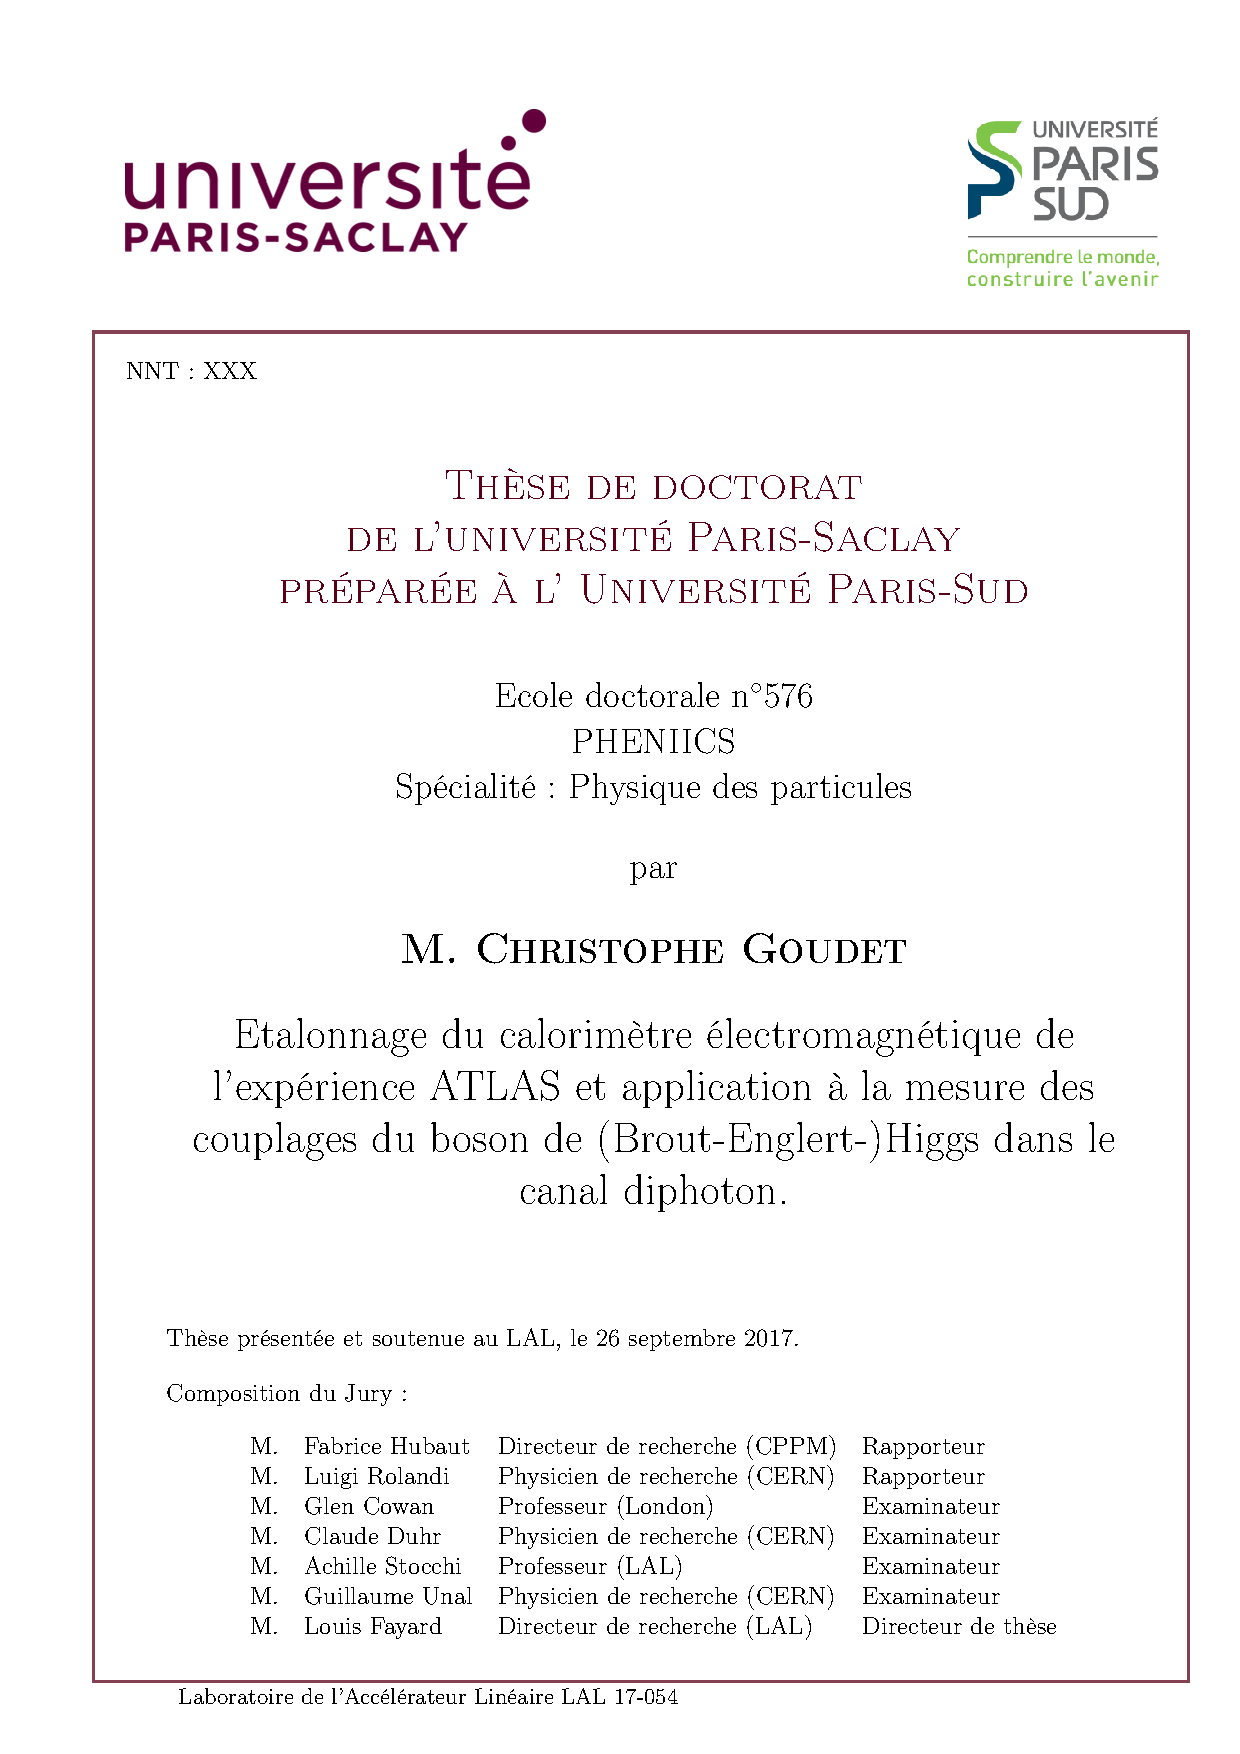
\includepdf[pages={1}]{PageDeGarde/cover.pdf}
\leavevmode\thispagestyle{empty}\newpage
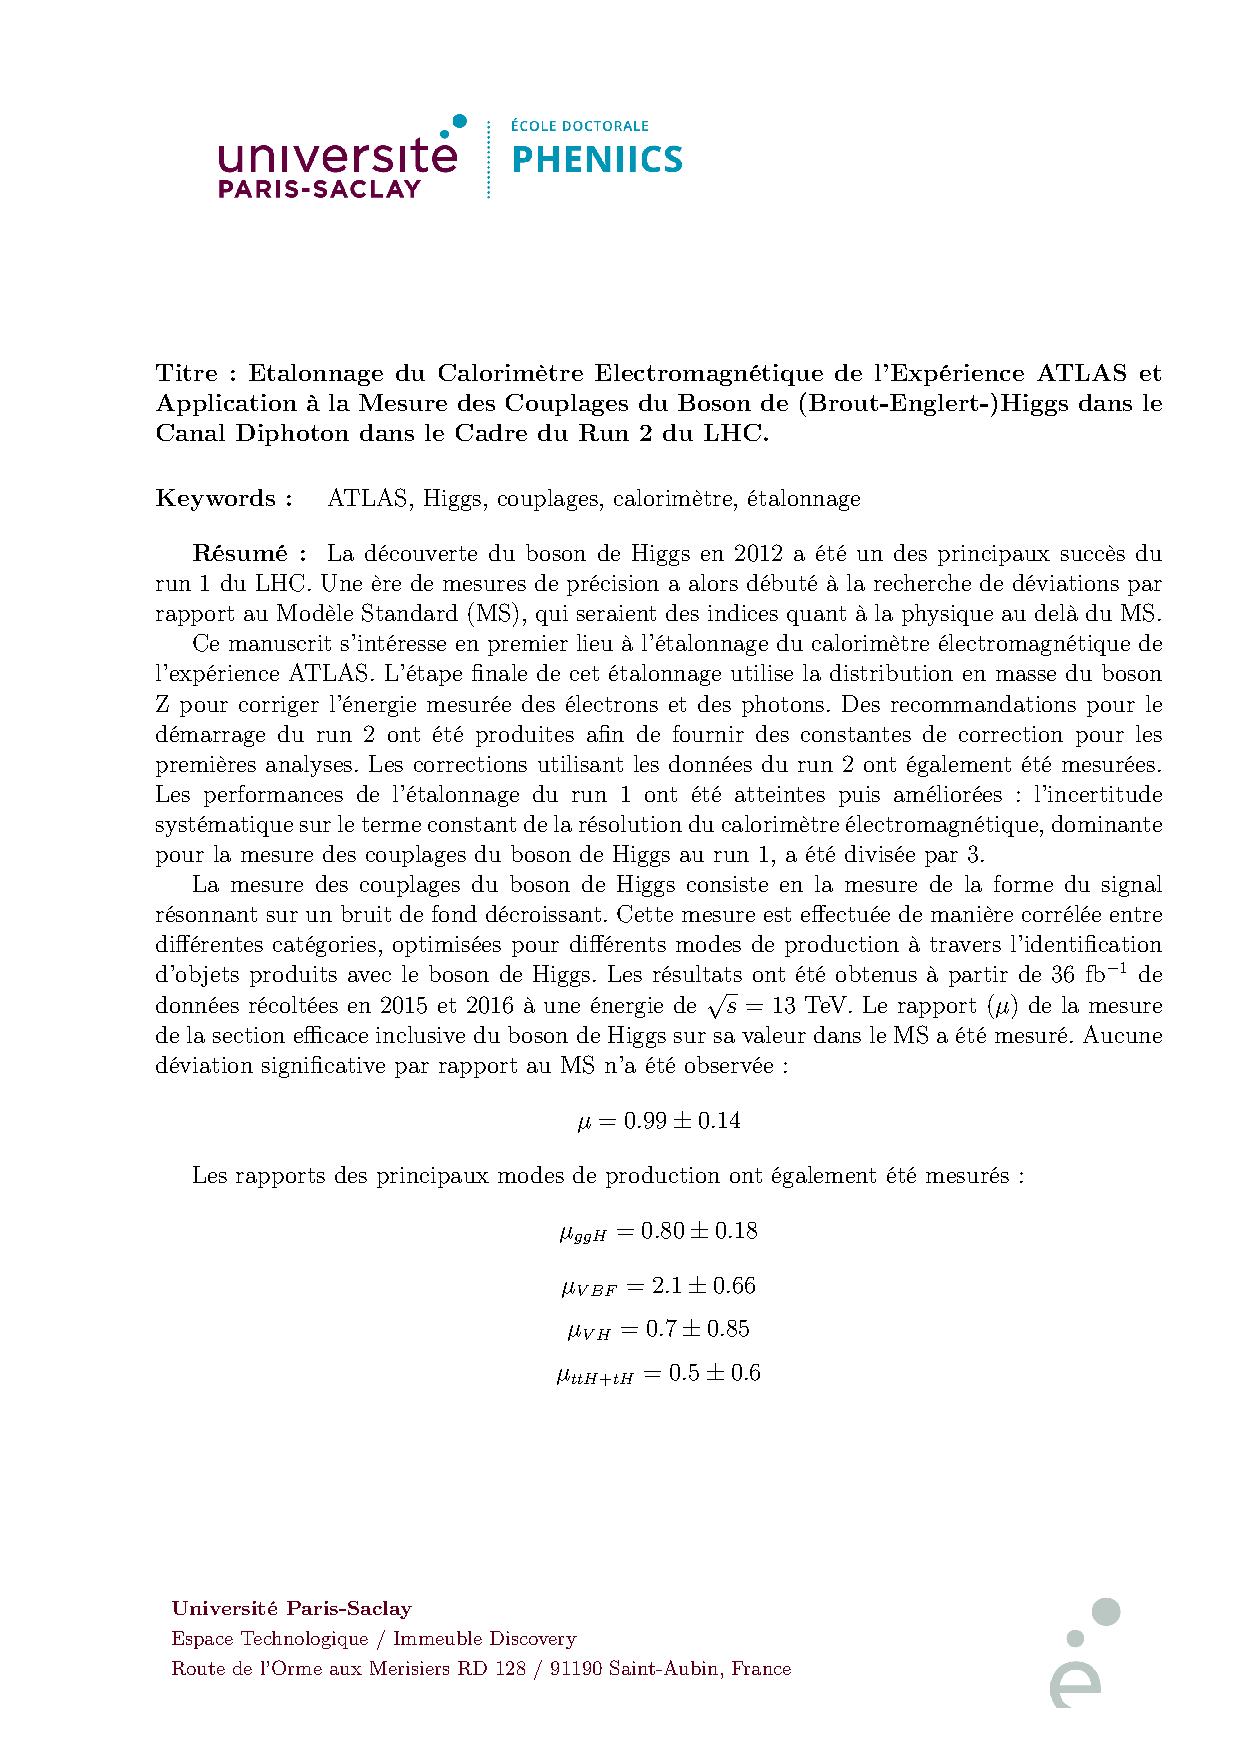
\includepdf[pages={1}]{PageDeGarde/absFr.pdf}
\leavevmode\thispagestyle{empty}\newpage
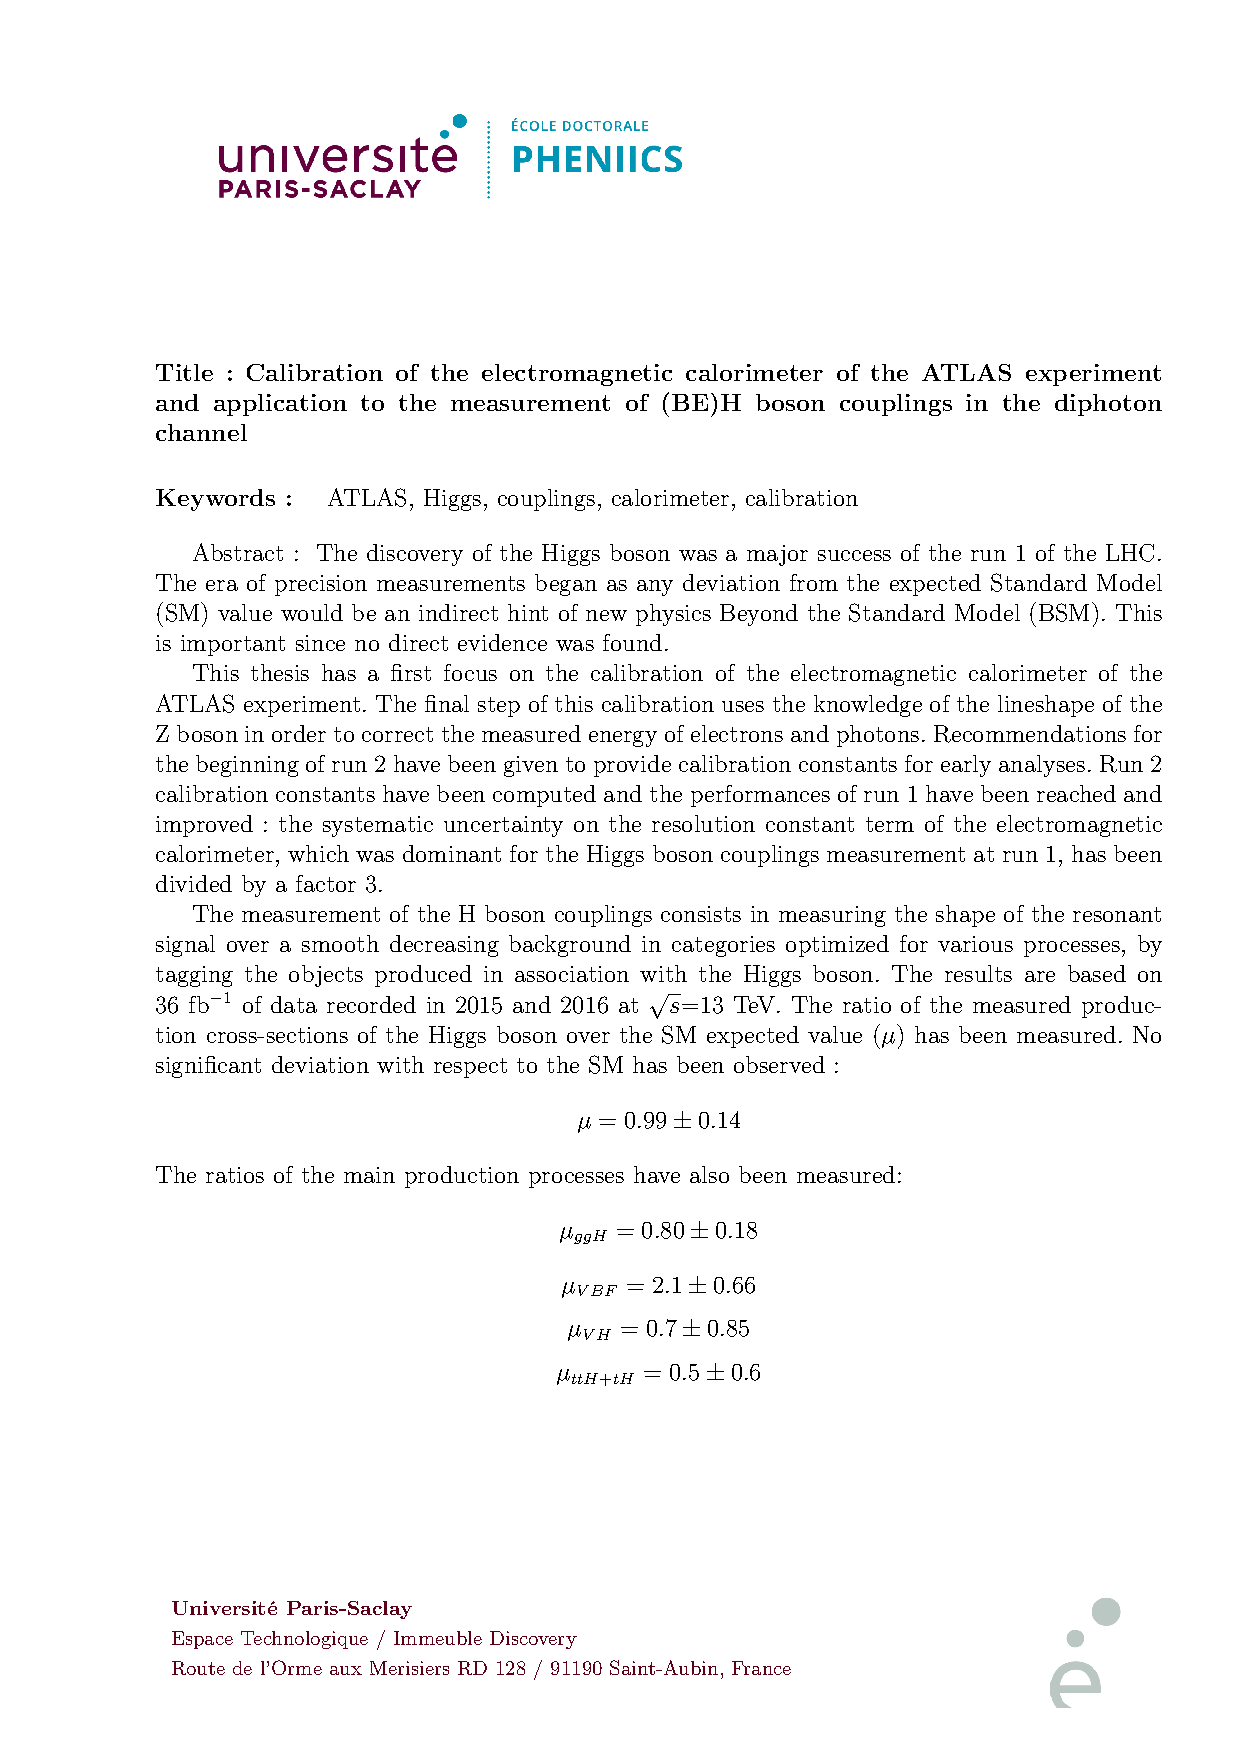
\includepdf[pages={1}]{PageDeGarde/absEn.pdf}

\frontmatter % Use roman page numbering style (i, ii, iii, iv...) for the pre-content pages

\pagestyle{plain} % Default to the plain heading style until the thesis style is called for the body content

%	QUOTATION PAGE
%----------------------------------------------------------------------------------------

\vspace*{0.2\textheight}

\noindent\enquote{\itshape
  Originally created by its inventor Trin Tragula as a way to get back at his wife (who was always telling him to get a ``sense of proportion''), the Vortex is now used as a torture and (in effect) killing device on the planet Frogstar B.
  The prospective victim of the TPV is placed within a small chamber wherein is displayed a model of the entire universe - together with a microscopic dot bearing the legend ``you are here''.
  The sense of perspective thereby conveyed destroys the victim's mind; it was stated that the TPV is the only known means of crushing a man's soul.
}

\hfill The Hitchhiker's Guide to the Galaxy

\hfill Douglas Adams


%----------------------------------------------------------------------------------------
%	LIST OF CONTENTS/FIGURES/TABLES PAGES
%----------------------------------------------------------------------------------------

\tableofcontents % Prints the main table of contents

%----------------------------------------------------------------------------------------
%	THESIS CONTENT - CHAPTERS
%----------------------------------------------------------------------------------------

\mainmatter % Begin numeric (1,2,3...) page numbering

\pagestyle{thesis} % Return the page headers back to the "thesis" style

% Include the chapters of the thesis as separate files from the Chapters folder
% Uncomment the lines as you write the chapters

\part{Theoretical context}
\label{sec:orgc95725b}
\chapter{A precise mathematical framework}
\label{sec:org5eabaf8}
\section{Historical overview}
\label{sec:org6825fe7}
Matter surrounds us at any time.
It is no surprise that it was one of the main topics of interest of philosophers, scientists or clerics.
Many conceptions have fought and succeeded each other to explain the nature of matter.
The antic greek philosophers had two explanations.
One hypothetized that if one cuts many times a sand grain in half, a piece which can not be reduced anymore can be obtained.
This piece has been called atom.
However, this theory mostly stayed in the shadow of the dominant theory which proclaimed for 20 centuries that matter was composed of the four elements (earth, wind, water and fire) in different composition depending on the type of material.
Alchemists of the western middle age also worked within this theory in order to be able to manipulate matter, without much successes.
The next major step in understanding the matter was due to $18^{th}$ century chemists who classified first materials and then elements with respect to their chemical properties.
Contrary to the previous theory that was proposed a priori, this new categorisation relied on observed properties and also proposed predictions.

The study of matter entered the era of modern scientific method.
The following century will see a huge increase in knowledge of matter.
Thomson proposed the atom as a sphere of positive charges in which light negative charges (the electrons) move.
A few years later, Rutherford will prove that the positive charges are actually concentrated in a very small volume, the nucleus : the modern conception of the atom was born.
The study of the newly discovered radioactive effect led to the hypothesis that the core of the atom was itself a combination of smaller constituents.
While the proton and the neutron were being discovered in 1919 and 1932, Pauli proposed a theory to explain the energy spectrum of electrons in beta decays which postulated the existence of a new particle : the neutrino.
At this point, the elementary constituents of ordinary matter were known but new kind of "rays" were observed : muons, pions, kaons, etc\ldots{} which were not part of the model.
In the 60's, Gell-Mann \cite{GellMann:1964nj} and Zweig \cite{Zweig:352337} proposed a framework in which the numerous proton-like particles which had been observed were combination of smaller parts, the quarks, which existence was confirmed several years later at SLAC \cite{Bloom:1969kc,Breidenbach:1969kd}.

The theory of matter went hand in hand with the observational results.
Mixing the two new theories of the beginning of the 20th century, quantum mechanics and special relativity, has given birth to quantum field theory to try to fit the matter knowledge into an elegant mathematical framework.
Observed structures were obtained by imposing symmetries on the system.
Perturbation theory allowed for easy computation of observable quantities.
Renormalisation removed divergencies in a full class of theories.
Symmetry breaking allowed to give some properties to particles which were forbidden by symmetries.
Many contributions which can not be all listed here led the theory of matter from a set of revolutionary ideas to a complex but elegant mathematical framework which yields a strong predictive power.

Finally, this cross improvement between theory and observation has been greatly improved with the performances of detectors.
120 years ago, Thomson discovered the electron by observing the light emitted by a gas when traversed by a charged current.
This equipment only allowed him to observe a macroscopic number of electrons.
But the development of cloud chambers and bubble chambers later changed that.
Now, one could directly detect a single particle, follow its trajectory and eventually witness its interactions.
Those visible marks could be photographed and many new particles were discovered by the interpretations of those pictures.
Finally, with the dawn of electronics, it was possible to detect and use very small electric signal created in a detector by a passing particle.
Using an always increasing precision, detectors allow us to "see" the trajectory of particles within them and then to reconstruct their "history".
In fig. \ref{org9494af2}, one can see a comparative of the available information at these three epochs.
This increase of technology also changed the way the observed particles are produced.
The first experiments were using the particles produced in the atmosphere or by radioactive decays.
Recently, developments in accelerator technology allowed for a less elegant but more effective particle production.
By smashing particles against each other and observing the results, we were able to observe more energetic and more rare processes in order to better probe our ignorance.

\begin{figure}
\begin{subfigure}[t]{0.32\linewidth}
\begin{center}
\includegraphics[width=\linewidth]{Cyclotron_motion_wider_view.jpg}
\end{center}
\end{subfigure}
\begin{subfigure}[t]{0.32\linewidth}
\begin{center}
\includegraphics[width=\linewidth]{20140712-neutral_current.jpg}
\end{center}
\end{subfigure}
\begin{subfigure}[t]{0.32\linewidth}
\begin{center}
\includegraphics[width=\linewidth]{run203602_evt82614360_vhres.png}
\end{center}
\end{subfigure}
\caption{\label{org9494af2}
Evolution of experimental output for particle physics over time. Left picture shows a glowing cathodic tube of 1900's. Central picture shows the tracks in a clound chamber in 1930's. Right picture show an event display in 2010's.}
\end{figure}


The Standard Model of particles (SM), which will be detailed later, is the current understanding of the matter, proposed in a well-defined mathematical framework.
The Large Hadron Collider (LHC) and its multi-billion Swiss francs investment among dozens of countries is a leading collaboration to probe this model and eventually identify hints of the next model to come.
Its main objective was to detect the last unseen particle of the SM, the Brout-Englert-Higgs (BEH) boson (sometimes called the Higgs boson, both terms will be used in this thesis).
With the detection of this particle in 2012, the SM is now complete.
The LHC and its four major experiments now aim at breaking the model by looking for discrepancies between data and predictions.
Up until now this task is more a failure as always improving precision measurements impressively follow the prediction over many energy scales of processes.


The search for physics beyond the SM (BSM) is mainly focused on three axes.
First, as was already mentioned, precision measurements may allow to observe discrepancies between data and predictions.
In particular, the existence of heavy particles not yet observed may have an indirect effect on measurable processes.
Secondly, some models propose new particles within direct reach of the LHC.
By directly searching the signature of those particles one can get a first direct entrance to the BSM physics.
Finally, the search for rare decays is a combination of the two previous cases.
Some processes in the SM suffers from very low (if not null) probability to happen.
However, some models predict an enhancement or an opening of some processes.
This axis then relies on the search of a SM signature which should not be observable.

This thesis will focus on the first axis as the objective is to measure the properties of the Higgs boson and compare them with its predicted values.
In this chapter I will present the theoretical framework of this analysis, namely the Standard Model and the Higgs mechanism.
The way in which the model is described depends a lot on the type of experimentation one performs.
This chapter will then conclude on the phenomenology of the Higgs boson in the SM at the LHC experiments.


\section{Gauge theories}
\label{sec:org5fbff7e}
\subsection{Least action principle}
\label{sec:org24ae533}

The formalism that will be developed in this chapter relies on the use of a Lagrangian.
This mathematical function represents the state of a system and depends on the space-time coordinates of the system (\(q_i\)) and their derivative (\(\dot{q_i}\)).
In classical mechanics, it is expressed as the difference between a kinetic term of the system and its interactions (or potential energy), as in eq. \ref{eq:orge6f59be} for a simple system.

\begin{equation}
\label{eq:orge6f59be}
L=T-V = \frac{m\vec{\dot{q}}^2}{2}-V(\vec{q})
\end{equation}

In the lagrangian formalism, the dynamics of a system is imposed by the least action principle.
The action is a functional which depends on the lagrangian according to eq. \ref{eq:org49905b5}.
The principle states that the system must follow a path in its phase space such that its action remains minimal.
Imposing the derivative of the action with respect to a coordinate to be null leads to the famous Euler-Lagrange equation (eq. \ref{eq:org97d0d1c}) which is used in practical cases.
This equation is widely used in classical mechanics and has a similar form in quantum field theory.

\begin{equation}
\label{eq:org49905b5}
S=\int L( q_i, \dot{q_i}) dt
\end{equation}

\begin{equation}
\label{eq:org97d0d1c}
\frac{\partial L}{\partial q} - \frac{d}{dt}\frac{\partial L}{\partial \dot{q_i}}=0
\end{equation}



\subsection{Symmetries}
\label{sec:org0eb9ce7}

A symmetry is a transformation that leaves a (physical) system invariant.
As an example consider a free particle following a straight trajectory.
If one changes the origin of the coordinates, hence performing a translation of the trajectory by a constant vector, the dynamics of the particle will remain the same.
Because the translation vector can take any real value in any direction, this symmetry is called continuous.
Similarly, observing the free particle a given day or the next should not change its trajectory.
The system is also invariant under time translation.
Continuous symmetries have an additional property : Noether's theorem \cite{Noether} states that they also conserve a quantity or current.
In the case of space translation, the quantity which is conserved is the momentum of the particle.
For time translation, the energy of the particle is conserved.

There exists a second class of symmetries : the discrete symmetries.
By opposition to continuous symmetries, the discrete symmetries are labelled by a finite or infinite set of integers.
An example of such symmetry is the parity : the transformation which changes a system into its image through a mirror.

So far, the symmetries mentioned consisted in a transformation of the space-time coordinates of the system.
Internal symmetries refer to transformations which do not affect the space-time coordinates.
They are heavily used in the quantum field theory in order to create inner structures of mathematical objects within the model.
Internal symmetries can be either discrete or continuous.


\subsection{Groups}
\label{sec:org18fff70}

A group is a set G of elements with a product law ( G, .) such that :
\begin{itemize}
\item for two elements g\(_{\text{1}}\) and g\(_{\text{2}}\) in G, g\(_{\text{1}}\).g\(_{\text{2}}\) belongs to G
\item there exists an identity element e such for any g in G, e.g = g.e = g
\item for three elements g\(_{\text{1}}\), g\(_{\text{2}}\) and g\(_{\text{3}}\) in G one has : \((g_1.g_2).g_3=g_1.(g_2.g_3)\)
\item if for g\(_{\text{1}}\), g\(_{\text{2}}\) \(\in\) G \(g_1.g_2=g_2.g_1\), then the group is called Abelian or commutative
\end{itemize}

A group can be representated by a set of matrices (a representation) with a 1 to 1 matching to all elements of the group.
The multiplication law of matrices must then reproduce the product law of the group such that :
\begin{equation}
g_1 . g_2 = g_3 \rightarrow M(g_1)\times M(g_2)=M(g_3)
\end{equation}
with M(g\(_{\text{i}}\)) the matrix associated with the member g\(_{\text{i}}\) of the group.

Groups of continuous symmetries are described using Lie groups.
The matrices elements of  a Lie group can be written as \(U=e^{\alpha_a T^a}\), where \(\alpha_{\text{a}}\) are continuous parameters and T\(^{\text{a}}\) are the generators of the Lie algebra of the group considered.
The commutation relations of the generators, usually written as \([T_a,T_b]=f^{abc}T_c\) where \(f^{abc}\) are called the structure constants, are sufficient to describe the full algebra of a Lie group.

Two types of Lie groups are often used in particle physics and will appear in the construction of the Standard Model : \(U(n)\) which consists in the set of \(n\times n\) unitary matrices such that \(|\text{det}(U)|=1\), and \(SU(n)\) which further imposes the determinant to be equal to 1.

\subsection{Gauge theories}
\label{sec:orga6a6451}
\begin{enumerate}
\item Dirac Lagrangian
\label{sec:org9b5a0cb}

Field theory proposes to describe the dynamics of fields in the same way particles are described in classical mechanics.
A field is a function of space-time coordinates \(\psi\)(q\(_{\text{i}}\),t) which can interact with external forces.
As in classical mechanics, one can define a Lagrangian of the field, which should be invariant under Lorentz transformations, and apply the least action principle in order to obtain the equations of motion.
One of the simplest cases is the Dirac Lagrangian :

\begin{equation}
\label{eq:orge86da29}
L = \bar{\psi}(i\slashed{\partial} -m)\psi
\end{equation}
where m is the mass of the particle described by the field \(\psi\) and
\begin{equation}
\begin{array}{l}
\bar{\psi} = \psi^\dagger \gamma^0\\
\slashed{\partial}=\gamma^\mu\partial_\mu
\end{array}
\end{equation}

The \(\gamma\) matrices are four dimensional objects which can be expressed in terms of the Pauli matrices.
\begin{equation}
\gamma^0=
\begin{pmatrix}
 \mathbbm{1} & 0 \\
0&  \mathbbm{1}
\end{pmatrix},
\gamma^k =
\begin{pmatrix}
 0&\sigma^k \\
-\sigma^k & 0
\end{pmatrix}
\end{equation}


A theory defined by this Lagrangian is not so interesting as it describes a single free moving field.
In order to enrich the theory, one can postulate symmetries that the theory must enforce : transformations on the fields such that the Lagrangian remains invariant.
A great variety of properties and phenomena must appear in the theory, depending on the imposed symmetries.
Later, the construction of the Standard Model will be detailed by expliciting those symmetries.
Equation \ref{eq:org3048dc4} proposes a continuous transformation independent of the space-time coordinates (global).
Because of the constant value of \(\alpha\) with respect to space time coordinates, the exponential isn't affected by the derivative term so this transformation is a natural symmetry of this Lagrangian.


\begin{equation}
\label{eq:org3048dc4}
\psi(x)\rightarrow e^{i\alpha}\psi(x)
\end{equation}

\item Gauge transformation
\label{sec:orgf786a4f}

One may wonder why we imposed \(\alpha\) to be a constant instead of the general case of a space-time dependent transformation.
Because of the derivative term in the Lagrangian, one can anticipate that such a transformation is not a natural symmetry of the theory, so imposing it may change the possible phenomena.
We'll leave aside the debate on the aesthetics of such a theory to focus on its consequences.
Let's first discuss the implications of such transformation in classical mechanics as proposed in \cite{Iliopoulos:1551844}.
Figure \ref{org992d083} shows the trajectory of a free particle before and after applying a global transformation consisting of a constant translation.
In this case, the trajectory remains a straight line.
In the second case, the translation vector is defined as position dependent.
The new trajectory is not anymore compatible with one of a free particle.
Instead, one can propose that this new trajectory corresponds to a particle under external forces.
With this interpretation, imposing a local symmetry leads to the creation of an interaction.

\begin{figure}
\begin{subfigure}[t]{0.49\linewidth}
\begin{center}
\includegraphics[width=0.9\linewidth]{Iliopoulos_1f.pdf}
\end{center}
\end{subfigure}
\begin{subfigure}[t]{0.49\linewidth}
\begin{center}
\includegraphics[width=0.9\linewidth]{Iliopoulos_2f.pdf}
\end{center}
\end{subfigure}
\caption{\label{org992d083}
Trajectory of a free particle after a global (left) and local (right) space translation. \cite{Iliopoulos:1551844}}
\end{figure}

Let's observe this concept in the case of our Dirac field theory by imposing the transformation in eq. \ref{eq:org07e9803}.
\begin{equation}
\label{eq:org07e9803}
\psi(x)\rightarrow e^{i\alpha(x)}\psi(x)
\end{equation}
Because the parameter \(\alpha\) is now space-time dependent, the derivative term will affect the exponential, hence leading to an additional term in the Lagrangian.
If one wants to impose the invariance of the Lagrangian under this transformation, one has to introduce an additional (gauge) field A\(_{\mu}\) in the system and replace the derivative operator by a co-variant derivative as in eq. \ref{eq:orgc79752f}.
When transforming the Lagrangian according to eq. \ref{eq:org07e9803}, the gauge field must transform according to eq. \ref{eq:orge69917a}.
\begin{equation}
\label{eq:orgc79752f}
\partial_\mu\rightarrow D_\mu=\partial_\mu+ieA_\mu(x)
\end{equation}
\begin{equation}
\label{eq:orge69917a}
A_{\mu} \rightarrow A_\mu(x) - \frac{1}{e} {\partial_{\mu} \alpha(x)}
\end{equation}
with e an arbitrary real constant.
Provided these transformation rules, the new Lagrangian is then invariant under the gauge transformation.
Finally, if we develop the Dirac Lagrangian with these new definitions, one gets eq. \ref{eq:orga0bf20e}.
Compared to our initial Lagrangian, this new version has an interaction term between the gauge field \(A\) and the fermion field \(\psi\).
The degrees of freedom of the field must then be included to complete the model.
Their form is uniquely determined by gauge invariance as in eq. \ref{eq:org5d97eb8}, which leads to the total Lagrangian expressed in eq. \ref{eq:org2698525}.


\begin{equation}
\label{eq:orga0bf20e}
L = \bar{\psi}(\slashed{\partial} - ie\slashed{A}_\mu(x)-m)\psi
\end{equation}

\begin{equation}
\label{eq:org5d97eb8}
F_{\mu\nu}(x) = \partial_\mu A_\nu(x) - \partial_\nu A_\mu (x)
\end{equation}

\begin{equation}
\label{eq:org2698525}
L = \frac{1}{4} F^{\mu\nu}(x) F_{\mu\nu}(x) + \bar{\psi}(x)(i\slashed{D}-m)\psi(x)
\end{equation}

\item Non-Abelian gauge transformation
\label{sec:orgaf7f151}

The class of transformations proposed so far can be represented by the group of unitary matrices \(U(1)\).
As can be seen from the equations, applying two successive transformations will lead to the same result, whatever the order.
\(U(1)\) is then called Abelian.
Again, one may wonder why we should restrict our theory to Abelian groups and the answer would be that we should not.
The calculations of the non-Abelian case are performed in detail in the literature and are not of interest in this discussion.
Applying non-Abelian local gauge transformations to the Lagrangian leads to additional derivative terms which can be removed by the addition of a set of additional gauge fields with appropriate transformation rules.
The QCD Lagrangian for instance then takes the form given in eq. \ref{eq:org215d25b}.

\begin{equation}
\label{eq:org215d25b}
L_{QCD} = \bar{\Psi}(i\slashed{\partial} - \frac{g_s}{2}\slashed{G}.t -m)\Psi - \frac{1}{4}Tr(G_{\mu\nu}G^{\mu\nu})
\end{equation}
where \(G_{\mu\nu}\) is the non-abelian equivalent of \(F_{\mu\nu}\), \(G\) the bosonic field of the theory, \(t\) the generators of the Lie group and $g_s$ an arbitrary real constant.
\end{enumerate}


\section{Spontaneous symmetry breaking}
\label{sec:orgf6a8fd0}
\label{sec:theory_SymBreak}
The mass is an intrinsic parameter of a field.
It appears in a Lagrangian in the form \(m\bar{\Psi}\Psi\).
Such terms are present for the fermionic field \(\psi\) in the theory we developed so far but not for the gauge field.
A mass term for the gauge field would appear as
\begin{equation}
-m^2A_\mu A^\mu
\end{equation}
which would not be invariant under the transformation of eq. \ref{eq:orge69917a}.
As a result, those terms are forbidden in the Lagrangian.

In 1933, Fermi proposed a model \cite{Fermi:1933jpa,Fermi2008} to explain the radioactivity with a direct interaction between a proton, a neutron, an electron and a neutrino, as shown in fig. \ref{fig:orgfa8568d}.
This model was limited to low energy as cross-sections computed in this framework diverged at high energy.
A way to remove this divergence was to remove the contact interaction and replacing it with a mediated one.
This is shown on the right part of fig. \ref{fig:orgfa8568d}, where the date 1938 corresponds to the proposal by Klein \cite{Klein:1938jm} of a boson exchange model for radiative decays, anticipating Yang-Mills theories \cite{Yang:1954ek}.
However, the mediator of the interaction should be massive and even extremely heavy with respect to the standards of the time.
Later data confirmed the theory of a heavy mediator with the indirect observation of neutral current by the Gargamelle experiment \cite{Gargamelle,Hasert:1973cr} and the discovery of \(W^{\pm}\) and Z\(^{\text{0}}\) at the \(\text{Sp}\bar{\text{p}}\text{S}\) at UA1 \cite{CERN-EP-83-13,1983398} and UA2 \cite{CERN-EP-83-25,CERN-EP-83-112}.

\begin{figure}[htbp]
\centering
\includegraphics[width=0.8\linewidth]{I15-06-FermiTheory.jpg}
\caption{\label{fig:orgfa8568d}
Diagrams representing the \(\beta\) decay in Fermi theory (left) and in weak interactions (right).}
\end{figure}


The solution came from BCS theory of supra-conductivity \cite{PhysRev.108.1175} which was able to give a mass term to photons by spontaneously breaking a symmetry in the ground state of their system.
The mechanism made its way into particle physics, in particular thanks to Nambu and Jona Lasinio \cite{Nambu:1961fr,Nambu:1961tp,Nambu:1960xd,Nambu:1960tm}, and was applied in abelian gauge theory by Brout and Englert \cite{BroutEnglert}, and Higgs \cite{Higgs64} independently.
The mechanism, applied to the electroweak interaction \cite{PhysRevLett.19.1264,SALAM1964168}, required a new particle in the theory which will later be the Standard Model : the so called (Brout-Englert-)Higgs boson (often called H).
Englert and Higgs won the Nobel prize in 2013 (Brout was deceased at that time) after the discovery \cite{CERN-PH-EP-2012-218,CERN-PH-EP-2012-220} of a resonance which properties are compatible with the Higgs boson the previous year at the LHC.


The mass-generating mechanism that will be loosely referred as Higgs mechanism relies on the assumption that the ground state of a system does not show the same symmetries that the Lagrangian from which it is derived.
Consider the simple example in fig. \ref{fig:orgc07deb6} in which a pencil is initially put vertically on a plane surface.
Classical mechanics tells us that this position is an unstable equilibrium so that the pencil will fall so as to reach a stable equilibrium.
The Lagrangian of the pencil was initially invariant under rotation around its axis.
In the final state, the pencil fell in one direction so space is not isotropic anymore.
The pen spontaneously left an unstable rotation-invariant state to go in a state with less symmetry.

\begin{figure}[htbp]
\centering
\includegraphics[width=0.6\linewidth]{SymBreakPen.jpg}
\caption{\label{fig:orgc07deb6}
Visualisation of a symmetry breaking with a pen at unstable equilibrium. \cite{SymBreakPen}}
\end{figure}

Let's consider this principle in a bosonic field theory invariant under the gauge transformation of eq. \ref{eq:org07e9803}.
The Lagrangian of the theory is enriched with a potential in the form given in \ref{eq:orgdea495d}.
Under the gauge transformation of the field \(\phi\), this potential is naturally invariant.

\begin{equation}
\label{eq:orgdea495d}
V(\phi) = \frac{1}{2}\mu^2\phi^*\phi+\frac{1}{4}\lambda(\phi^*\phi)^2
\end{equation}

If \(\lambda\) is negative, the potential does not have a lower bound : the system is unstable.
For \(\lambda\) and \(\mu^{\text{2}}\) positive, the minimum of the potential is at \(0\) so the ground state respects the symmetry of the potential.
Finally, for negative \(\mu^{\text{2}}\), the potential allows for a non trivial minimum.
In the case of a complex field, there is an infinite number of generated minima defined by \(\{ve^{i\alpha}, \alpha\in R\}\) as shown in fig. \ref{fig:org609c856}.
\(v=\sqrt{-\frac{\mu^2}{\lambda}}\) is the vacuum expectation value.
The system must choose spontaneously one ground state among the available minima, hence leaving its trivial symmetric initial one.


\begin{figure}[htbp]
\centering
\includegraphics[width=0.6\linewidth]{MexicanHatPot.jpg}
\caption{\label{fig:org609c856}
Potential for U(1) symmetry breaking. \cite{1DPotential}}
\end{figure}

Consider that the system chooses the minimum \(\phi_0=v+i\times 0\).
A generalisation can be easily performed by rotating the system.
The dynamic of the theory is obtained by perturbation theory around this minimum.
One can re-parametrize the two degrees of freedom of the field around the ground state using eq. \ref{eq:org3984bfe}.

\begin{equation}
\label{eq:org3984bfe}
\phi(x)=\frac{v +\sigma(x)+i\pi(x)}{\sqrt{2}}
\end{equation}

This new parametrization is then injected into a bosonic \(U(1)\) gauge theory.
Some computation leads to the following form for the Lagrangian.
\begin{equation}
\label{eq:orgf74cc7a}
L = \frac{1}{2}|\partial_\mu\sigma|^2 + \frac{1}{2}|\partial_\mu\pi|^2 -v^2\lambda\sigma^2 +  - \lambda( \pi^2\sigma^2 + 2 \pi^2 v \sigma ) - \frac{\lambda}{2}(\sigma^4+\pi^4 + 4v\sigma^3) + C
\end{equation}
where C is a calculable constant.

The first two terms are the kinetic terms for the two degrees of freedom.
The third term is proportional to \(\sigma^{\text{2}}\) : it a mass term for this field.
The \(\sigma\) field characterises the excitation in the radial direction, as energy is required to climb the walls of the potential.
On the other hand, there is no quadratic term in \(\pi\).
This field corresponds to the lateral excitation of the field which needs no energy to go from a minimum to any other one because of the degeneracy.
The presence of this mass-less boson is the result of a theorem demonstrated by Goldstone \cite{PhysRev.127.965}.
This theorem states that for every spontaneously broken continuous symmetry there should be a mass-less scalar boson.
These bosons have not been observed.
This issue may be solved by the Higgs mechanism in a local gauge invariance.

Finally, the initial gauge theory for radioactivity imposed mass-less gauge bosons as a price for mathematical elegance (and precision of physical predictions).
However, it was quickly understood that gauge bosons had to be massive and even very heavy for the experiments to be understood.
Finally, using spontaneously broken symmetry, imported from condensed matter, allowed for massive gauge bosons.
This improvement is at the price of adding the scalar Higgs boson to the theory


\section{The Standard Model}
\label{sec:orga563bf8}

\subsection{Construction of the SM}
\label{sec:orgb0b6048}

The main ingredients to create a gauge theory have been presented.
The Standard Model and most Beyond Standard Model (BSM) theories are only different recipes.
To summarise, a gauge theory is built by following those steps :
\begin{itemize}
\item choosing the group invariances,
\item choosing the particle content of the theory (fermions),
\item including (or not) one or many symmetry breaking mechanisms and corresponding fields.
\end{itemize}

There is a vast choice of gauge invariances available for gauge theory.
While restricting to (special) unitary groups, the possibilities in term of combinations are limitless.
The choice between abelian and/or non-Abelian groups may give rise to a wide variety of phenomena.
The only constraint on the choice in our case is the possibility to interpret observed phenomena.
In the case of the SM, the lagrangian is imposed invariant under \(SU(3)_c\times SU(2)_I\times U(1)_Y\).
The particles (fields) which will be included later will then have as property a combination of color (c), hypercharge (Y) and isospin (I), which will impose their behaviour under each gauge invariance.
\(SU(3)\) group will manage the strong interaction.
It is a non-abelian group which is defined by 8 generators which will translate into 8 massless gauge bosons : the gluons.
\(SU(2)_I\times U(1)_Y\) will be responsible for the electroweak sector.
This non-abelian group will generate 4 electroweak gauge bosons : the charged bosons \(W^{\pm}\), and the two neutral \(Z^0\) and photon (\(\gamma\)).
The gauge group is often written \(SU(3)_c \times SU(2)_L \times U(1)_Y\) since SU(2) acts only on left chiral fermions.

The particle content of the theory is mostly arbitrary.
However, the easiest way to be in agreement with the experimental results is to add fields corresponding to some observed states.
Additional fields can be added to fulfil the philosophy of the theory.
Finally, fields can be added a posteriori to the theory in order to tune some phenomena.
In the SM, 12 fermion fields are injected in the theory along with the Higgs field.
The remaining boson states arise due to gauge invariances.
The fermions form two groups of equal size (6 fermions in each) : quarks and leptons.
The former will be sensitive to all gauge interactions while the latter only to the electroweak part.
In each group, the fermions are paired.
For the leptons (quarks), members of the pair will be either charged or neutral (up or down types).
Finally there exist a hierarchy between pairs, with ranks called family.
The quark and lepton pair of the same rank are labelled as part of the same family : leading to a total of 3 families.
Fig. \ref{fig:org1db6618} proposes a visualisation of this organisation of fermions.
The first family consist in fields which make ordinary matter : up and down quarks combine to create protons and neutrons, and electron (and electronic neutrino).
The second family is composed of the charm and the strange quarks, the muon and the muonic neutrino.
Every particle of the second family is identical to its counterpart in the first family but with a higher mass.
While not part of ordinary matter, the second family is "naturally" present as muons are heavily produced in the upper atmosphere (although they decay rapidly).
The third family is made of particles identical to the second family but with higher masses : top and bottom quarks, \(\tau\) lepton and tau neutrino.

\begin{figure}[htbp]
\centering
\includegraphics[width=0.8\linewidth]{OPEN-PHO-CHART-2015-001.png}
\caption{\label{fig:org1db6618}
Qualitative particle content of the Standard Model. \cite{OPEN-PHO-CHART-2015-001}}
\end{figure}

Spontaneously symmetry breaking is heavily used in BSM theories, for instance in supersymmetry.
The Standard Model only breaks the electroweak symmetry in order to give a mass term to electroweak bosons.
Choices have been made both in term of the representation for the Higgs field but also on the shape of the potential.
The SM chooses the simplest potential as in section \ref{sec:theory_SymBreak}.
Still, two free parameters remain, \(\lambda\) and \(\mu\), so they will be set to values obtained from by data.
Since the measurement of the Fermi constant G\(_{\text{F}}\), which is related to weak bosons masses, a constraint is set on the vacuum expectation value of the potential.
Until 2012, no more information was available to constraint the system.
Indirect searches and theory asumptions only reduced the available phase space.
The mass of the Higgs boson was necessary to complete the model.
Direct searches were performed successively by LEP, Tevatron and finally LHC.
Finally in 2012 the last parameter of the SM could be measured.

\subsection{Electroweak sector}
\label{sec:orga4e442f}

The lifetimes involved in weak interaction are significantly higher than ones for strong interaction.
Indeed, weak radioactive decays constant times are of the order of the second or higher while strong interaction barely last longer than 10\(^{\text{-14}}\)s.
These long lifetimes were attributed to a weaker interaction, hence its name.
After some developments, it turned out that the couplings of the weak interaction were of the order of the electromagnetic coupling.
The weakness of the interaction was then attributed to large masses of the vector bosons which mediated the interaction.

The electroweak theory is imposed invariant under the gauge symmetry \(SU(2)_I\times U(1)_Y\).
This symmetry imply the presence of 4 gauge bosons : 3 for SU(2) (W\(^{\text{i}}_{\mu}\)) and 1 for U(1) (B\(_{\mu}\)).
The covariant derivative has the following formula :

\begin{equation}
\label{eq:orgb1ab3fc}
D_\mu = \partial_\mu - i\frac{g}{2}\sigma_i.W_\mu^i - i\frac{g'}{2}YB_\mu
\end{equation}
with \(\sigma\) the Pauli matrices, $g$ and $g'$ two arbitrary real constants.

\begin{enumerate}
\item Higgs sector
\label{sec:org4acdc8d}

The representation chosen for the Higgs field is a SU(2)\(_{\text{L}}\) complex doublet with a hypercharge \(Y=1\).
Its most general form is
\begin{equation}
\Phi =
\left(
\begin{array}{l}
\phi^+\\
\phi^0\\
\end{array}
\right)
= \frac{1}{\sqrt{2}}
\left(
\begin{array}{l}
\phi_1 + i \phi_2\\
\phi_3 + i \phi_4\\
\end{array}
\right)
\end{equation}
with \(\phi_{\text{i}}\)'s properly normalised real scalar fields.

The dynamic of the Higgs field is described by the Lagrangian :
\begin{equation}
L_H = (D_\mu\Phi)^\dagger (D^\mu \Phi) - \mu^2 \Phi^\dagger \Phi - \lambda (\Phi^\dagger\Phi)^2
\end{equation}

The minimum potential of this field is a four dimensional sphere such that :
\begin{equation}
\Phi^\dagger \Phi = \frac{1}{2}(\phi_1^2+\phi^2_2 +\phi_3^2 + \phi_4^2) = - \frac{\mu^2}{2\lambda} = \frac{v^2}{2}
\end{equation}

The Higgs field can be re-parametrized around the minimum \(<\phi_3>=v\) and \(<\phi_1>=<\phi_2>=<\phi_4>=0\).
A specific choice of gauge, called the unitary gauge lead to :
\begin{equation}
\Phi = \frac{1}{\sqrt{2}} \left(
\begin{array}{c}
0\\ v+h \\
\end{array}
\right)
\end{equation}


Combining the covariant derivative formula with the expression of the Higgs field in the unitary gauge, the kinetic term of the Higgs field takes the form :
\begin{equation}
(D_\mu\Phi)^\dagger (D^\mu \Phi)
= \frac{1}{2}(\partial_\mu h)(\partial^\mu h)
+\frac{1}{8}(v+h)^2 \left[ g^2(W_\mu^1-iW_\mu^2)(W^{1\mu} + iW^{2\mu}) + (-g'B_\mu + g W^3_\mu)^2 \right]
\end{equation}

The first term correspond to the properly normalised kinetic term for the real scalar field h.
The first part of the second term correspond to the charged boson \(W^\pm\) which are defined such that
\begin{equation}
W_\mu^\pm = \frac{W_\mu^1 \mp iW_\mu^2}{\sqrt{2}}
\end{equation}
Developing this term leads to the expression of the mass term for these bosons :
\begin{equation}
m_W = \frac{vg}{2}
\end{equation}

The last term can be identified with the interaction of the Z boson with the Higgs mass.
It is a linear combination of the third generator of SU(2) and the generator of U(1).
Properly normalised, this field and its orthogonal take the form :

\begin{equation}
\begin{array}{l}
Z_\mu = cos \theta_W W^3_\mu - sin\theta_W B_\mu\\
A_\mu = cos\theta_W B_\mu + sin \theta_W W_\mu ^3 \\
cos \theta_W = \frac{g}{\sqrt{g^2+g'^2}}\\
sin \theta_W = \frac{g'}{\sqrt{g^2+g'^2}}\\
\end{array}
\end{equation}

The field A\(_{\mu}\) is not coupled to the Higgs fields hence will not have a mass term.
This field is identified with the photon.
The mass term for these two fields finally take the form :
\begin{equation}
\begin{array}{l}
m_Z = \frac{v\sqrt{g^2+g'^2}}{2} = \frac{m_W}{cos \theta_W}\\
m_A=0
\end{array}
\end{equation}


\item Fermions representation
\label{sec:org1416521}

In the electroweak theory, the W boson interacts only  to the "left" component of the fermions, which corresponds to the projection of the field using the operator \(P_L = \frac{1}{2}(1-\gamma_5)\).
The left components of the fermion fields are then organised into two doublets and the right components are assigned to singlets.
Finally, the fermion fields will be defined as follow :

\begin{equation}
L_l^i= P_L
\begin{bmatrix}
    \nu_i(x) \\
    l_i(x) \\
\end{bmatrix}
; \
L_q^i= P_L
\begin{bmatrix}
    u_i(x) \\
    d_i(x) \\
\end{bmatrix}
; \ i=1,2,3
\end{equation}

\begin{equation}
R_f(x) = (1-P_L) \psi_f(x)
\end{equation}
with f representing any fermion (from any family).

Right handed neutrino have no interaction with the electroweak sector (and the strong sector) and as such can be removed from the SM.

Finally, the leptonic sector of the electroweak theory takes the form.
\begin{equation}
L\supset i\bar{L}_l\gamma^\mu D_\mu L_l +  i \bar{R}_l\gamma^\mu D_\mu R_l
\end{equation}

No mass term is present is this lagrangian.
As for the weak bosons, it will be generated by their interaction with the Higgs field.
The only possible solution, given the choice of Higgs boson representation, is a Yukawa coupling between fermions and the Higgs field.

\begin{equation}
L_{\text{Yukawa,l}} \supset - \left[ y_l \bar{R}_l \Phi^\dagger L_l +y_l^*\bar{L}_l\Phi R_l  \right]  = -\left( \frac{y_l v}{\sqrt{2}}\right) \bar{L_l}R_l - \frac{y_l}{\sqrt{2}} h\bar{L_l}R_l + \text{h.c.}
\end{equation}
where y\(_{\text{l}}\) is the dimensionless couplings of the lepton to the Higgs boson.
The second step of the equation is obtained with the Higgs field in the unitary gauge.

A similar approach for the quarks would lead to a mass term only for the up type quark.
The issue can be solved if the conjugate of the Higgs field \(\tilde{\Phi}=i\sigma_2\Phi\) is used instead.
The total interaction term of the quark field from the first family with the Higgs fields then takes the form :
\begin{equation}
L_{\text{Yukawa,Q}} \supset - [ y_u \bar{R}_u \Phi^\dagger L_u + y_d \bar{R}_d \tilde{\Phi}^\dagger L_d + h.c.]
\end{equation}

The discussion about fermion parametrization focused on the first family.
The two other families are parametrized in the same way as the first.

\item Quarks mixing
\label{sec:org603067f}

The quark mixing is another characteristic of the weak interaction.
Cabibbo \cite{CERN-TH-342} proposed in 1963 that the quark eigen-states for the weak interaction were different from the mass eigen-state.
This allowed the weak interaction to change the flavour of quarks.
This model has been extended by Kobayashi and Maskawa in 1973 \cite{KUNS-242}.
Within this model, the mass eigen-states (d', s', b') are related to the interaction eigen-states by the CKM matrix :

\begin{equation}
\begin{pmatrix}d\\s\\b\end{pmatrix}
= V_{CKM}
\begin{pmatrix}d'\\s'\\b'\end{pmatrix}
\end{equation}

with :
\begin{equation}
V_{CKM}=
\begin{pmatrix}V_{ud}&V_{us}&V_{ub}\\V_{cd}&V_{cs}&V_{cb}\\V_{td}&V_{ts}&V_{tb}\end{pmatrix}
\end{equation}
\end{enumerate}

\subsection{Higgs boson production and decay predictions at the LHC}
\label{sec:org649229c}

The strength of a model is the precision at which it describes observed phenomena but also mainly its ability to predict new phenomenon.
The spontaneous symmetry breaking formalism allows in an elegant framework to provide a mass to fermions and weak bosons at the cost of a new (scalar H) boson.
One prediction of the theory lies in the properties of this new particle and in its interactions with the other particles of the SM.

The Higgs boson theoretical predictions at the LHC are summarised in ref. \cite{CERN-2013-004}.
This document details the level of precision as well as assumptions included in the computation of various Higgs boson properties.
An overview of the production and decay of the H boson is proposed in the following sections.

The mass of the H boson is the only free parameter of the SM to be determined after the discovery of the top quark \cite{Abe:1995hr} so properties of the boson can only be computed as a function of its mass.
Before the LHC, the various electroweak measurements \cite{LEPEWWG} and the direct LEP limits \cite{CERN-EP-2003-011} restrained the mass of a light H boson to be within [114, 152] GeV at 95\% CL.
Even within this limited range, its properties have large variations depending on its mass.
The discussions on production modes and decay width will include the mass dependence in order to propose a broad view of the context at the start of the LHC.
Since the measurement of the H boson mass \cite{CERN-PH-EP-2015-075}, the paradigm has evolved to a situation where properties have only small variations between masses in the measured confidence interval.



\begin{enumerate}
\item Production modes
\label{sec:org52a585f}

At the LHC, proton collisions allow for a large variety of interactions.
Indeed, through the sea (with quarks and gluons) of the proton, important at this energy, one can consider virtually all type of quarks and gluon as initial states of processes.
Therefore, several processes leading to the creation of a Higgs boson are accessible.
Fig. \ref{fig:org34d1e6a} presents the H boson cross section (as a function of its mass) of  the main production processes for protons colliding at a center of mass energy of \(\sqrt{s}=14\) TeV.


\begin{figure}[htbp]
\centering
\includegraphics[width=0.8\linewidth]{YRHXS_Summary_fig3.pdf}
\caption{\label{fig:org34d1e6a}
Inclusive Higgs boson production cross-section as a function of its mass at $\sqrt{s}=14$ TeV at the LHC. \cite{CERN-2013-004}}
\end{figure}


Five production processes are considered to give a measurable contribution to the total cross-section within the run 2 of the LHC.
These processes, which diagrams are shown in fig. \ref{fig:org3ec611e}, differ by the partons required in the initial state but also of the particle content present in the final state along with the H boson.
It is then possible to infer the process which produced a Higgs  boson by the study of the rest of the event.
This is the target of the coupling measurements.


\begin{figure}[htbp]
\centering
\includegraphics[width=0.7\linewidth]{CERN-THESIS-2014-122_1f10.pdf}
\caption{\label{fig:org3ec611e}
SM Higgs boson leading order production processes at the LHC. \cite{CERN-THESIS-2014-122}}
\end{figure}

The dominant mode at the LHC is the fusion of gluons (ggH).
Like for most of the processes the ggH cross section was first computed at the leading order, corresponding to the top left diagram of fig. \ref{fig:org3ec611e}.
However, this leading order approximation is in many cases insufficient, and large uncertainties derive from its dependence on the unphysical renormalisation and factorisation scales.
Next to leading order (NLO) computation were done in the finite top mass approximation \cite{Spira:1995rr} and then N$^2$LO and N$^3$LO computations were done \cite{CERN-PH-TH-2015-055,CERN-TH-2016-006} in the infinite top mass limit.
One sees in fig. \ref{CERN-TH-2016-006_8f} that the dependence of the cross section on a common renormalisation and factorisation scale decreases when higher orders are used.
The latest computation of the ggH inclusive cross section gives $\sigma_{\text{ggH}} = 48.58 ^{+4.56\%}_{-6.72\%}\ \text{(theory)}\ \pm 3.2\ \text{(PDF + }\alpha_s\text{)}$ pb at $m_H=125$ GeV at a center of mass energy of 13 TeV.
It represents roughly 86\% of the total Higgs boson cross-section.
It is interesting to notice that this process contains a loop of heavy quarks (mainly top but with a small contribution of bottom and charm) at leading order.
It has been decided (\cite{deFlorian:2227475} section 1.9) for the couplings analysis to consider this theory uncertainty as a 100\% flat interval.
Since one wants to have a Gaussian uncertainty, the interval was symmetrized and the ``Gaussian'' standard deviation is $(6.7+6.7)\% /\sqrt{12} = 3.9\%$.

\begin{figure}[h!]
  \centering
  \includegraphics[width=0.7\linewidth]{CERN-TH-2016-006_8f.png}
  \caption{Dependence of the ggH cross section on a common renormalisation and factorisation scale. \cite{CERN-TH-2016-006}}
  \label{CERN-TH-2016-006_8f}
\end{figure}

The second most important production mode is the vector boson fusion (VBF) which is initiated by quarks radiating weak bosons which fuse into a Higgs boson.
This process accounts for about 10\% of the total cross-section.
It is particularly interesting as it probes the coupling of the Higgs boson to the gauge bosons.
Furthermore, this production process can be differentiated from the main ggH production by the two quarks in the final state which will create two forward jets.
Tagging those jets is the core concept of VBF coupling measurement.
The two following production modes also probe the coupling of the Higgs boson with electroweak bosons : WH and ZH, also called Higgstrahlung, both result from a production of a weak boson which will radiate a H.
The weak boson which remains in the final state can also be tagged.

Finally, H can be produced by the interaction of a pair of top quarks.
This production process mode has a lower cross-section than the previous ones and has some similarities with the VBF process, as a top pair is also present in the final state and create a jet.
The study of this production process rely on identifying jets produced by bottom quarks produced by the decay of the top quarks.
The ttH production has a dedicated analysis in ATLAS.


With the increase of the energy of the LHC in 2015 up to 13 TeV, the production cross-sections of many reactions (including Higgs boson production) increase.
Fig. \ref{fig:org96cd9f6} shows the ratio between the 13 TeV cross section and the 8 TeV for a set of processes.
It shows that even for the Higgs boson, this ratio is different depending on the production mode : ranging from 2.0 for WH to 3.9 for ttH.
Finally, this increase of energy plays a major role in the improvement of measurement of the Higgs boson properties, in particular for the identification of the ttH production mode.

\begin{figure}[htbp]
\centering
\includegraphics[width=0.8\linewidth]{crossSectionRatio-13-8TeV.pdf}
\caption{\label{fig:org96cd9f6}
Ratio of processes cross-section for colliding protons at \(\sqrt{s}=13\) TeV with respect to 8 TeV for a set of processes. Credit : A. Hoecker}
\end{figure}


\item Decay channel
\label{sec:orgf4c19b0}

The Higgs boson is not a stable particle and will quickly decay into a variety of final states.
Its total width as a function of its mass is given in fig. \ref{fig:org26dfcff}.
Above 160 GeV, the total width quickly increases as new decay channels fully open.
This could have been problematic as most search analyses rely on observing a narrow resonance over the background.
On the contrary, a light Higgs boson would have a width so small compared to the detector resolution(\(\simeq 2\)  GeV) that it would be difficult to measure it.
The observation favours the latter case : at 125 GeV the SM Higgs boson width is predicted to be 4.1 MeV.

\begin{figure}[htbp]
\centering
\includegraphics[width=0.5\linewidth]{YRHXS_BR_fig2.pdf}
\caption{\label{fig:org26dfcff}
Width of the SM Higgs boson as a function of its mass. \cite{CERN-2013-004}}
\end{figure}

The set of available decay channels heavily depends on the mass of the boson.
Figure \ref{fig:org6c93d9f} shows the branching ratio for different decays as a function of the mass.
Given the constraints on the Higgs boson mass imposed by LEP and TEVATRON, most of the decay channels presented in fig. \ref{fig:org6c93d9f} were good candidates for measurements.
A large variety of analyses were then possible in order to constraint the Higgs boson properties.

\begin{figure}[htbp]
\centering
\includegraphics[width=0.5\linewidth]{higgs_br.pdf}
\caption{\label{fig:org6c93d9f}
Standard Model Higgs boson branching ratio as a function of its mass. \cite{CERN-2013-004}}
\end{figure}

At 125 GeV, the leading decay channel is \(b\bar{b}\).
This channel is a priori the most promising as the leading one with about 58\% of branching fraction.
However, its final signature is a pair of jets which suffers a large background in an hadronic collider, even when identifying b jets.
As a result, the search of bottom decay of the Higgs boson is mainly limited to the Higgsstralung production mode (see fig. \ref{fig:org3ec611e}) in order to use the weak boson signature to reduce the background.
This decay channel was not observed at a 3$\sigma$ level in run 1 in ATLAS \cite{ATLAS-CONF-2013-079,CERN-PH-EP-2014-214} or in ATLAS+CMS \cite{CERN-EP-2016-100}.
However, a recent ATLAS analysis \cite{CERN-EP-2017-175,CERN-EP-2017-175} of combined run 1 and run 2 data shows a measured (expected) significance of 3.6(4.0)$\sigma$.
An even more recent preliminary CMS analysis \cite{CMS-PAS-HIG-16-044} shows a measured (expected) significance for the combined run 1 and run 2 of $3.8(3.8)\sigma$.

The gluon decay channel, along with $c\bar{c}$ decay, is not observable.
Indeed, the experimental signature of these decays is only a pair of jets, which is widely produced in an hadronic collider.
However, the diagram of the gluon decay is the same as the gluon fusion production process but inverted.
The information of the effective couplings of gluons to the Higgs boson is then already present in the H boson cross-section.

The Higgs boson decay into a tau or muon pair is an opportunity to probe the Higgs boson couplings to leptons.
ATLAS run 1 analysis observed an excess of $4.5\sigma$ (wrt null hypothesis) in the tau decay channel \cite{CERN-PH-EP-2014-262}.
This level of excess is compatible with the SM.

The decay of the H boson into a pair of weak bosons has a large branching ratio.
However, the bosons will themselves decay into various stable particles.
The most promising channel in term of identification is a decay into a pair of Z bosons which themselves decay into a pair of leptons.
This channel is extremely rare due to the leptonic branching ratio of the Z boson (3.363\% \cite{PDG2016}) but this is compensated by a low level of background.
This channel contributed to the discovery of the H boson and remains a leading one for measurement of its properties.


The \(H\rightarrow \gamma\gamma\) channel has peculiar characteristics.
It suffers from a very low branching ratio (\(\simeq 2.10^{-3}\)) which makes it rare.
However the final state, two isolated photons, can be efficiently detected by an electromagnetic calorimeter.
Given that the background has a monotonous shape, the H signal can be observed above the background.
This particular decay is described by the diagrams in fig. \ref{fig:org310104c}.
Even at the leading order, it consists in a loop of t and b quarks and of W boson.
This allows to probe the couplings to these particles and brings additional complementary information to other dedicated channels.
Finally, since the decay is done through a loop, this process is sensitive to the contribution of heavy BSM particles inside the loop so contributes to indirect BSM searches.

\begin{figure}[htbp]
\centering
\includegraphics[width=0.8\linewidth]{CERN-THESIS-2014-122_1f9.pdf}
\caption{\label{fig:org310104c}
Leading order Feynman diagrams of SM Higgs boson decay to a photon pair. \cite{CERN-THESIS-2014-122}}
\end{figure}
\end{enumerate}


\section{LHC results}
\label{sec:orgf76e3ba}

The LHC primary goal was to provide conditions for the observation of the source of electroweak symmetry breaking (the Higgs boson in the SM) and to search for BSM particles in the two general purpose experiments.
It is also a great instrument at which to probe the SM and precisely measure its parameters and its consistency.
Some tests of the SM are provided in fig. \ref{fig:org87b5838}.
It is impressive to see that the SM is able to predict phenomena through 14 orders of magnitude.


\begin{figure}[htbp]
\centering
\includegraphics[width=\linewidth]{ATLAS_b_SMSummary_FiducialXsect.pdf}
\caption{\label{fig:org87b5838}
Compatibility of various measured cross-section with SM prediction. \cite{ATLASSMTest}}
\end{figure}


The major highlight of the run 1 of the LHC was the discovery by ATLAS and CMS collaborations of the Higgs boson.
This observation was driven by three decay channels : \(H\rightarrow\gamma\gamma\), \(H\rightarrow ZZ^*\rightarrow 4l\) and \(H\rightarrow WW^* \rightarrow l\nu l\nu\).
Since then, the measurement of the mass of the resonance has been performed for each decay channel available as well as a combined one \cite{CMS-HIG-14-009,CERN-PH-EP-2014-122}.
ATLAS and CMS decided to combine \cite{CERN-PH-EP-2015-075} their results in order to get a single LHC mass measurement.
This combination of four measurements (diphoton and four leptons for each experiment) took place with approximately 25 fb\(^{\text{-1}}\) in each experiment.
The results for each measurement and for the combined ones are shown in fig. \ref{fig:orga7ceb32}.
The final LHC run 1 Higgs boson mass measurement is  \(m_H = 125.09 \pm 0.21 \text{(stat.)} \pm 0.11 \text{(syst.)}\).
Since then, a compatible measurement by CMS of the Higgs boson mass in the 4l channel of \(m_H=125.26\pm0.21=125.26 \pm 0.20\ \text{(stat)}\ \pm 0.08\ \text{(syst)}\) GeV occurred \cite{CMS-PAS-HIG-16-041,CMS-HIG-16-041}.

\begin{figure}[htbp]
\centering
\includegraphics[width=0.7\linewidth]{CERN-PH-EP-2015-075_2f.pdf}
\caption{\label{fig:orga7ceb32}
Review of Higgs boson mass measurement in ATLAS and CMS at run 1. \cite{CERN-PH-EP-2015-075}}
\end{figure}

The couplings of the H to various particles is related to the masses of the decay particles.
As these measurements have already been performed, the SM is in principle complete.
However, the newly discovered Higgs sector can probe BSM effects.
It is then of major importance to try and measure all these couplings, including the effective ones containing loops, so as to spot any possible deviation from the theory.
 Both ATLAS \cite{ATLAS-CONF-2015-007} and CMS \cite{CMS-HIG-14-009} measured the ratio ($\kappa$) of the measured couplings with respect to the SM ones.
A combination of both experiments \cite{CERN-EP-2016-100} has been performed which main results are presented in fig. \ref{fig:orgfd66e48}.
No significant deviation from the SM is observed.

\begin{figure}[htbp]
\centering
\includegraphics[width=0.7\linewidth]{CERN-EP-2016-100_18f.pdf}
\caption{\label{fig:orgfd66e48}
ATLAS and CMS combined measurement of couplings deviation from the Standard Model for the run 1 of LHC. These results assume no invisible decay of the Higgs boson, no decay to BSM particles and no BSM particles in the loops. \cite{CERN-EP-2016-100}}
\end{figure}

Direct and indirect measurements of the Higgs boson width have been performed.
The direct measurement rely on testing an hypothetized value of the width and fitting the invariant mass distribution by a convolution of the detector resolution and a Breit-Wigner representing the signal propagator.
The results of this measurement \cite{CERN-THESIS-2015-193,CERN-PH-EP-2014-122} set the upper limit on $\Gamma_H$ of a few GeV.
The recent result of CMS \cite{CMS-PAS-HIG-16-041,CMS-HIG-16-041} gives $\Gamma_H < 1.1$ GeV at 95\% Confidence Level (CL).
This direct model independent methodology does not bring much constraint on Higgs boson properties due to the large detector resolution with respect to the signal width.
An indirect model-dependent method was proposed \cite{Dixon:2013haa} to use the on-shell interference between the \(H\rightarrow\gamma\gamma\) signal and the background.
In addition, the interference of Higgs 4l decay off-shell signal with the background can also be used to make indirect model dependent limits, as proposed in \cite{Caola:2013yja}.
With this method, one can set an indirect limit on the Higgs boson width by comparing the signal yield within and outside the peak in the 4 leptons and WW channels.
With this method ATLAS \cite{ATLAS-CONF-2014-042,CERN-PH-EP-2015-026} was able to constrain the width to $\Gamma_H <22.7$ MeV at 95\% CL.




\section{Conclusion}
\label{sec:org69deba1}
The dawn of quantum field theory allowed for a common elegant mathematical framework able to describe the observed behaviour of the matter.
The Standard Model of particle physics has been tested to an impressive precision.
However, several observed phenomenon can not be explained in this context.
The SM does not include information about dark matter, dark energy, or neutrino oscillation for example.
New theories are then developped Beyond the Standard Model (BSM) in order to describe both the SM and those new effects.
Most of the current proposed theories are build on the same mathematical framework as the SM, but with different symmetries, particle content and/ord symmetry breakings.
Constraints on BSM physics are searched through either the direct observation of new resonnances or by indirect observation of deviations from the SM.
So far the last observed prediction of the SM, the Higgs boson, is fully compatible with the expectations.
The challenges for run 2 and beyond of the LHC will be to reduce statistical and experimental uncertainties to probe the Higgs boson parameters at the percent level.

\chapter{Statistics}
\label{sec:orgc8635b2}

The statistical treatment of the data is the transition between the experimental measurement of quantities and the interpretation of the collected data into a theory.
This interpretation usually aims at determining the values of a set of parameters of the theory (parameters of interest \(\vec{\mu}\)) which best describe the data.
The inputs of the statistical framework are a set of events for which observables have been measured \(\{\vec{x_e}\}\).
The procedure will rely on the determination of the probability to observe the data under the assumption of a given model \(P(\{\vec{x_e}\}| \vec{\mu})\).


\section{Model building}
\label{sec:orgf5f8572}

The modelling of the problem is performed by the creation of a likelihood, i.e. a function which quantifies the level of agreement between the data and a given theory.
In a simple cut and count analysis, the model predicts an amount of observed events K by combining the tested theory and experimental considerations.
The probability of observing N events when K are expected, which is equivalent to the agreement between data and the model, follows a Poisson distribution.
\begin{equation}
P_K(N)=\frac{K^N}{N!}e^{-K}
\end{equation}

Usually, a set of observable quantities are measured for each event and can be used to improve the statistical model.
The probability to observe the observables \(\vec{x_e}\) is defined by the model, using either MC simulations, data driven techniques or analytic forms.
This distribution takes into account the correlations between all the variables.
If there are no correlations, the total probability density function (PDF) is simply the product of the individual PDF of each observable.
Finally, the probability to observe the dataset \(\{\vec{x_e}\}\) is the product of the probabilities to observe each event.
The total likelihood $f(\{\vec{x_e}\})$ is finally the combination of the Poisson probability and the product of PDF for the observables.
\begin{equation}
f(\{\vec{x_e}\}) = \frac{K^N}{N!}e^{-K} \prod\limits_{e=1}^{N} f(\vec{x_e})
\end{equation}

The dependence of the likelihood with respect to the underlying theory has been kept implicit so far.
For two different models, the number of expected events and the PDF of the observables are model dependent.
Usually, the  theories tested against each other belong to the same class of theories and can be indexed by a set of parameters of interest (POI) \(\vec{\mu}\).
The number of expected events and the PDF of the observables usually depends on \(\vec{\mu}\), which allows to differentiate theories.

In particle physics events are usually classified into two categories : the signal which is a process that the analysis tries to observe or measure, and the background which represents known processes.
In the cross-section measurement of the H boson, the tested models differ only by the amount of signal events (S) that is expected in the analysis.
These signal events are then mixed in the analysis with background events for which we will assume we have a (almost) perfect knowledge.
The set of observables in this analysis is reduced to the distribution of the reconstructed invariant mass of the diphoton system, parametrized as a weighted average of the PDF of the signal and the background.
The difference in expected yields between models is then translated in the statistical model into a difference in the shape of the mass distribution.
In this context, the probability to observe the data under the assumption of S signal events takes the form :
\begin{equation}
f({\vec{x_e}} | S) = \frac{(S+B)^N}{N!}e^{-(S+B)} \prod\limits_{e=1}^{N} \frac{S f_S(\vec{x_e}) + Bf_B(\vec{x_e})}{S+B}
= \frac{1}{N!}e^{-(S+B)} \prod\limits_{e=1}^{N} (S f_S(\vec{x_e}) + Bf_B(\vec{x_e}))
\end{equation}
where f\(_{\text{S}}\) and f\(_{\text{B}}\) are the expected mass pdf distribution of the signal and the background, and B the expected background yield.

A single analysis is usually optimised and the selection of events removes some part of the signal in order to better reject background.
There may be a region in the remaining phase space from where signal information could also be extracted.
It is then interesting to combine the information from both analyses in order to reach signal constraints stronger than from either of the individual analyses.
Furthermore, an analysis is usually optimised for a reduced set of POI.
A more complete model could be created by combining different analyses which target different POI.
A combination of these multiple analyses, then referred as categories, is obtained by multiplying the corresponding likelihood together.
The correlations between analyses in taken into account by identifying common parameters between categories.
In run 1, H boson mass measurement was performed by combining 10 categories with different resolutions and signal significances.

In large datasets, it can become expensive in term of computing power to compute the likelihood (and especially to maximise it).
Instead of considering the probability to observe each event separately, it is possible to replace the PDF of observables by histograms.
The expected number of event in each bin (as a function of \(\vec{\mu}\)) can be computed as the integral of the PDF of the observable over the bin width.
A likelihood equivalent  for un-binned events is achieved by considering each bin as a simple cut and count analysis and combining all of them.


\section{Uncertainties treatment}
\label{sec:org9cc7929}
\label{sec:stat_NP}

The statistical model depends on parameters of interest but also on external inputs, the nuisance parameters (NP), for which one does not have a perfect knowledge.
They can be the result of an experimental measurement, or being an uncertain theoretical parameter.
Most of those parameters take the form of correction or re-weighting factors measured on dedicated analyses, such as the energy scale factors which are applied on photons and electrons and which are measured using $Z\rightarrow ee$ analysis (see sec. \ref{sec:Calibration_calibration}).

A proper modelling of the data must consider the uncertainties on those nuisance parameters by combining the statistical model with the auxiliary measurement.
Many analyses do not have a sufficient knowledge of the background so measure the background in control regions where no signal is expected.
The information on the background is included in the statistical model by considering the control region as a category and correlating the background parameters between the control and the signal region.
However in the H boson to diphoton analysis, background shape and yield are measured in the side-bands of the data.

The auxiliary measurement may not use a similar statistical procedure to measure parameters most probable values (MPV) and uncertainties.
It may then not be possible to easily combine it with the statistical model.
Instead, the performances of the auxiliary measurement are simplified into a probability density function for the nuisance parameter and combined with the main model.
Usually it is assumed that this constraint is a Gaussian function, centred on the MPV of the NP, and with a RMS equal to the total uncertainty of the NP.


In practice, a NP is $\eta$ and $p_T$ dependent and affect each event differently.
Depending on the properties of its selection, each category has a different effective dependency on a nuisance parameter.
As a result, each category should impose its own Gaussian constraint on a NP, with complicated correlations with other categories.
The likelihood of a category which depends only on a single NP \(\chi\), with MPV \(\chi^{\text{0}}\) and an uncertainty \(\delta\),  takes the form :
\begin{equation}
\label{eq:org6dd9827}
L_{tot} = L(\chi)e^{-\frac{(\chi-\chi_0)^2}{2\delta^2}}
\end{equation}


Usually, correction factors parameters do not appear explicitly in the likelihood as it parametrizes the corrected data.
The parametrization proposed in eq. \ref{eq:org6dd9827} can not be used as the \(\chi\) parameter may not appear explicitly in the model.
Instead, the change of variable proposed in eq. \ref{eq:org97da222}  allows to include the same information in the statistical framework but with a major simplification.
The Gaussian constraint is now only dependent on a parameter \(\theta\) which represents the deviation of the parameter NP, in units of its uncertainty, with respect to its MPV.
The information about the deviation is also included into the category by the multiplicative term $(1+\delta \theta)$.
Without any category dependent variable, all Gaussian constraints are not identical and can be merged into a single global constraint.
Finally, this parametrization can be used in the case where the NP is effectively absorbed into another variable as its MPV is not required anymore.
\begin{equation}
\label{eq:org97da222}
\chi \rightarrow \chi_0 (1+\delta\theta); \ e^{-\frac{(\chi-\chi_0)^2}{2\delta^2}} \rightarrow e^{-\frac{\theta^2}{2}}
\end{equation}


The estimation of the POI and NP which best describe the data is performed by maximising the likelihood (or in practice minimising -2ln(L)).
Auxiliary measurements are usually dedicated analyses with optimal sensitivity.
It is not expected that the data of a Higgs boson measurement for instance contribute significantly to the NP determination.
On the contrary, it is expected that the value of the NP showing the best agreement with data is close to its nominal value, meaning \(\theta\)=0.
Similarly, the constraining power of the data on the NP is expected to be negligible with respect to the one of the dedicated auxiliary measurement.
Hence, only the Gaussian constraint should have a contribution on the uncertainty of the NP, which implies an uncertainty of 1.
A coherence check is performed after minimisation to ensure that the NP have the expected best value and uncertainty.
An illustration of such a check, performed on an Asimov, can be seen for a set of NP in the $H\rightarrow\gamma\gamma$ couplings analysis in fig. \ref{fig:orgc0d4446} where the black markers represent the measured values for the \(\theta\)'s of selected NP.


\begin{figure}[htbp]
\centering
\includegraphics[width=0.7\linewidth]{ATL-COM-PHYS-2016-1784_168f.pdf}
\caption{\label{fig:orgc0d4446}
Ranking of nuisance parameters on an Asimov dataset (see sec. \ref{sec:org561a813}) in the \(H\rightarrow\gamma\gamma\) couplings analysis. The black markers represent central pull and overconstraints of NP.\cite{ATL-COM-PHYS-2016-1784}}
\end{figure}


The parametrization in eq. \ref{eq:org97da222} allows the parameter \(\chi\) to be negative.
This may be unphysical for some parameters such as the detector resolution or selection efficiencies.
The constraint on the parameter \(\chi\) is then changed to a log-normal (eq. \ref{eq:org2163697}) which prevent any negative value of the parameter.
\begin{equation}
\label{eq:org2163697}
\text{logNorm}(\chi; \chi_0, \sigma) = \frac{1}{\chi} exp \left( - \frac{(ln (\chi/\chi_0))^2}{2\sigma'^2}   \right) \simeq C exp \left( - \frac{(ln (\chi/\chi_0))^2}{2\sigma'^2} \right)
\end{equation}
A re-parametrization, shown in eq. \ref{eq:orgedde977} of the likelihood is performed in the same spirit as for the Gaussian constraint by defining \(\theta = \frac{1}{\sigma'} ln(\chi/\chi_0)\).
\begin{equation}
\label{eq:orgedde977}
\chi\rightarrow\chi_0e^{\theta\sigma'}; \ exp \left( - \frac{(ln (\chi/\chi_0))^2}{2\sigma'^2} \right) \rightarrow e^{-\frac{\theta^2}{2}}
\end{equation}
In practice, the change of constraint is then limited to a change of the multiplicative factor in the likelihood.
\(\sigma\)' is related to \(\delta\) by imposing the RMS of the log-normal function to be equal to the uncertainty on \(\chi_{\text{0}}\).
One must then solve :
\begin{equation}
\delta^2 = e^{\sigma'^2}(e^{\sigma'^2}-1)
\end{equation}


Finally, the log-normal constraint is obtained by changing the \(\chi\) parameter with
\begin{equation}
\label{eq:org9060827}
\chi\rightarrow\chi_0 e^{\theta\sqrt{ln\left(\frac{1+\sqrt{1+4\delta^2}}{2}\right)}} \simeq \chi_0 e^{\theta\sqrt{ln(1+\delta^2)}}
\end{equation}


\section{Compatibility measurement}
\label{sec:orga82e3f9}
\label{sec:stat_confidenceInterval}
\subsection{Confidence interval}
\label{sec:org30ef1ce}

In a measurement, one wants to find values of the parameters of interest (\(\vec{\mu}\)) which are compatible up to a certain level with the data and eventually the values which show the best agreement.
The most probable value is obtained by maximising the likelihood over the set of parameters of interest (\(\vec{\mu}\)) and the nuisance parameters (\(\vec{\theta}\)).
The construction of a confidence interval is detailed in the case of a single POI \(\mu\) and no NP.
The generalisation with a more complex likelihood is mentioned later.

An exclusion region at the level of \(\alpha\) defines an ensemble of values of \(\mu\) such that the probability to observe them under the tested hypothesis is smaller than \(\alpha\).
% The definition of the exclusion region is arbitrary.
From the probability distribution of the observed \(\mu\) under the assumption of \(\mu_{\text{test}}\), one can arbitrarily decide the definition of the exclusion region as long as the integral of the distribution over this region is equal to $\alpha$.
Two definitions are widely used, depending on the objective of the analysis.
The one-sided case assumes that all incompatible values are the extreme values on a single side of the distribution with respect to \(\mu_{\text{test}}\).
The exclusion region is defined as all values of \(\mu\) above (or below) \(\mu_{\text{0}}\) such that \(|\int\limits_{\mu_0}^{\pm\infty}f(\mu|\mu_{test})|=\alpha\).
On the other hand, the two-sided method shares equally the \(\alpha\) probability between both sides of \(\mu_{\text{test}}\).
The exclusion region is then defined as \(]-\infty,k]\cup[k',+\infty[\)  such that \(\int\limits_{k'}^{+\infty}f(\mu|\mu_{test})=\int\limits^{k}_{-\infty}f(\mu|\mu_{test})=\alpha/2\).
A visual representation of these two definitions is proposed in fig. \ref{fig:org6ce2637}.

\begin{figure}[htbp]
\centering
\includegraphics[width=0.6\linewidth]{OneTwoSided.jpg}
\caption{\label{fig:org6ce2637}
Visualisation of the two-sided (left) and one-sided (right) exclusion regions of size \(\alpha\)=5\%.}
\end{figure}

Using this definition of exclusion region, Neyman proposed in 1937 a method to define confidence intervals \cite{Neyman333}, which have a probability $\beta=1-\alpha$ of containing the true value of \(\mu\).
For each tested \(\mu_{\text{test}}\) one looks if the observed \(\mu_{\text{obs}}\) falls into the rejection region.
If so, \(\mu_{\text{test}}\) is considered not compatible with the data and is rejected from the confidence interval.
If \(\mu_{\text{obs}}\) does not fall in the rejection region, \(\mu_{\text{test}}\) is kept in the confidence interval \cite{PDG2016}.
A visualisation of this construction is proposed in fig. \ref{fig:org410e477} for the case of an observable x representative of an underlying theory parameter \(\theta\).

\begin{figure}[htbp]
\centering
\includegraphics[width=0.6\linewidth]{CERN-2015-001-247_4f.pdf}
\caption{\label{fig:org410e477}
Sketch of the Neyman contruction of confidence interval. \cite{CERN-2015-001-247}}
\end{figure}

The construction of Neyman becomes more complicated to visualise in practical case of many POI and observables.
A test statistic is then used to translate all of the information into a real number.
The usual test statistic used for measurement in LHC experiment is the profile likelihood ratio :
\begin{equation}
\label{eq:org444fadf}
t_{\vec{\mu}} = -2ln \left(\frac{L(\vec{\mu},\hat{\hat{\vec{\theta}}})}{L(\hat{\vec{\mu}},\hat{\vec{\theta}})} \right) = -2ln(\lambda(\vec{\mu}))
\end{equation}
\(\hat{X}\) is the value of X which allows the best agreement with data (i.e. maximises the likelihood).
\(\hat{\hat{\theta}}\) is the value of $\theta$ which maximises the likelihood under some conditions, usually fixing the value of \(\vec{\mu}\) ( see \cite{Cowan:1071727} for instance).
The value of $t_\mu$ is null for the best agreement between the model and data, and increases with further disagreement.
No differentiation is done between disagreements above and below the tested value so this test statistic corresponds to a two-sided confidence interval.
Depending on the type of confidence interval one wants to create, different definitions of profiles likelihoods are possible.
Practical examples for analyses in particle physics are proposed in \cite{Cowan:1071727}.


The test statistic formalism allows to reduce the determination of possibly complicated rejection region, into a simple one-sided rejection region on a single variable (\(t_{\vec{\mu}}\)).
Fig. \ref{fig:org571b725} shows an illustration of the distribution of a similar test, q\(_{\mu}\), under two different hypotheses of true \(\mu\) : either identical with the one tested or different.
If one computes the distribution of the test statistic for events corresponding to the same \(\mu\) than the one used in the test statistic, (i.e. this is what we would see if we compute the agreement between data and the true theory), there is a larger probability to observe a low value (good agreement), hence the $t_\mu$ distribution has larger probability close to zero.
On the contrary, if the \(\mu\) of the test statistic and of the events tested are different, there is in average a larger disagreement between the data and the distribution of $t_\mu$ is peaked at a large value.

\begin{figure}[htbp]
\centering
\includegraphics[width=0.6\linewidth]{Cowan_1007_1727_2f.pdf}
\caption{\label{fig:org571b725}
Illustration of q\(_{\mu}\) distribution under the different hypothesis.\cite{Cowan:1071727}}
\end{figure}

The definition of the confidence interval for $\vec{\mu}$ is derived from the definition of a rejection region for $t_{\vec{\mu}}$.
From the distribution of $t_{\vec{\mu}}$ under the hypothesis of $\vec{\mu}_{\text{test}}$, one can define t\(_{\text{0}}\) such that \(\int\limits_{t_0}^{+\infty}f(t_{\vec{\mu}}|\vec{\mu}_{test})=\alpha\).
This correspond to the set of measurements which are the least compatible with the model.
This region is represented in blue in fig. \ref{fig:org571b725}.
If the value of the observed \(t_{\vec{\mu}_{test}}\) is larger than t\(_{\text{0}}\), then the hypothesis $\vec{\mu}_{\text{test}}$ is rejected.
Otherwise, \(\mu_{\text{test}}\) belongs to the confidence interval.
By scanning the available phase space of \(\vec{\mu}\), the confidence interval is created by keeping the values for which the observed test statistic does not belongs to the rejection region.


\subsection{$t_\mu$ distribution}
\label{sec:orgf0b767b}

In the description of the confidence interval there was no mention of how to compute the distribution of $t_{\vec{\mu}}$ under a $\vec{\mu}_{\text{test}}$ hypothesis \(f(t_{\vec{\mu}}|\vec{\mu_{test}})\).
Two methods are widely used in particle physics.

The first method consists in the generation of pseudo experiments called toys.
For each toy, one must generate random pseudo-data according to a model ($\vec{\mu}_{\text{test}}$) to simulate "data" one would obtain by performing again the experiment.
The set of generated toys aims at being representative of the statistical fluctuations of the data.
The $t_{\vec{\mu}}$ of each toy can be computed by fitting the toy dataset with the statistical model.
The distribution of $t_{\vec{\mu}}$ can be unveiled by a sufficiently large amount of toys.

The statistical fluctuation of the toys are obtained by randomly generating the number of event observed in each bin using a Poisson distribution.
The cost of the method is linked to the rejection power (\(\alpha\)) one wants to achieve : an analysis rejecting at 5\% or 0.01\% will not have the same requirements on tail description, hence in the number of toys required.
In any case, the method is intrinsically expensive in term of cpu as one has to generate a large number of dataset and fit (twice) the statistical model over it.
In the case of complex models, the fitting procedure can itself be extremely time consuming (hours or days).
Examples of very time consuming toys can be found in section 5.4 of \cite{CERN-THESIS-2015-193}.
Because of the cost, this method is mostly used for analyses for which the distribution differ significantly from a Gaussian and for which no lighter procedure would give correct results.


While the current cpu capacities usually allow to consider the toy method, alternate solutions to obtain the distribution of $t_{\vec{\mu}}$ where studied both because of lack of cpu at the time and to save time for simple cases.
Following the results of Wilks \cite{wilks1938} and Wald \cite{Wald1943}, an analytic formulation of the problem was proposed in the case of large statistics.
The procedure is detailed in the context of particle physics in \cite{Cowan:1071727}.
Under the assumption of large statistics (N), $\mu$ is expected to have a Gaussian distribution and $t_{\mu}$ is a function of the estimator of the parameter and its uncertainty only :
\begin{equation}
\label{eq:org68bb290}
t_\mu = -2ln\lambda (\mu) = \frac{(\mu - \hat{\mu})^2}{\sigma^2} + O(1/\sqrt{N}).
\end{equation}
When neglecting the term \(O(1/\sqrt{N})\), the $t_\mu$ distribution follows a noncentral chi-square distribution for one degree of freedom (eq. \ref{eq:org8849c5a}).
The shape of the $t_\mu$ distribution was also computed for models with more parameters of interest in \cite{Cowan:1071727} : in that case the distribution follows  a non-central chi-square distribution for r degrees of freedom.
The knowledge of the analytical form of \(f(t_{\vec{\mu}}|\vec{\mu}')\) allows to easily compute its cumulative distribution which is then used to define the rejection region.
As a result the confidence interval can be obtained by studying this single function instead of generating a large amount of toys.

\begin{equation}
\label{eq:org8849c5a}
 f(t_\mu | \mu' ) = \frac{1}{\sqrt{8\pi t_\mu }} \left[ \text{exp} \left( -\frac{1}{2} (\sqrt{t_\mu} + \frac{\mu - \mu'}{\sigma})^2\right)  + \text{exp}\left( -\frac{1}{2} (\sqrt{t_\mu} - \frac{\mu - \mu'}{\sigma})^2\right)\right]
\end{equation}


\subsection{Practical cases}
\label{sec:org48c544d}

The construction of confidence interval presented so far is mostly theoretical and practical uses differ.
One common way of estimating the confidence interval in the Gaussian approximation is to compute the covariant matrix V\(_{\text{ij}}\) of the maximum likelihood.
This uses the well known equation :

\begin{equation}
V_{ij}^{-1} = - \frac{\partial^2ln(L)}{\partial \theta_j \partial \theta_k }
\end{equation}

By indexing \(\mu\)=\(\theta_{\text{0}}\), the confidence interval is defined as \([\hat{\mu}-\sqrt{V_{00}}, \hat{\mu}+\sqrt{V_{00}}]\).
This computation is performed by the MINUIT \cite{James:873119} algorithm.
In the case a of Gaussian distributed variable, this interval corresponds to the values within one standard deviation from the centre, and corresponds to a 68\% confidence interval.
In the case of a confidence region in two or more dimensions, one has to take into account the off-diagonal terms in the covariance matrix to ensure a proper coverage of the true values.
This method, which gives symmetric uncertainty on the POI, can not be used in cases of non-symmetric distributions.

Usually, physicists use only eq. \ref{eq:org68bb290} to define the confidence interval, so still using Gaussian assumption.
Assuming \(\hat{\mu}\) is the true value, one can compute the $t_\mu$ for \(\mu \neq \hat{\mu}\) and obtain the \(\sigma\).
In practice at the LHC, one displays the curve of $t_\mu$ as a function of \(\mu\) which in the Gaussian assumption is a positive parabola which is minimal at \(\hat{\mu}\) as in fig. \ref{fig:org31eaacd}.
The curve is usually shifted in order to match its minimum with 0.
Eq. \ref{eq:org68bb290} tells us that the borders of the 68\% confidence interval are values of \(\mu\) such that \(\mu-\hat{\mu}=\sigma\) hence $t_\mu=1$.
Similarly, the 95\% confidence interval is bounded by $t_\mu=4$
\footnote{Actually, $t_\mu=4$ for the 95\% confidence interval is an approximation.
  The 95\% confidence interval of a Gaussian is defined as $\mu\pm1.96\sigma$, which lead to $t_\mu=1.96^2=3.84$.
Both definitions are commonly used.}.
While more graphically oriented, this method allows to see the shape of the minimum which is probed and eventually observe up/down asymmetries.
Usually, it is assumed that the method is still reliable for large asymmetries such as in fig. \ref{orgb73d0b1}.
This methods also allows for visualisation of several minima in the likelihood provided some small constraints in the choice of initial state of the fit.
A typical example of plot showing two minima is also provided in fig. \ref{orgb73d0b1}.
Finally, in the case of several parameters of interest, one can scan their phase space and plot the contour line for which $t_\mu$ reaches the relevant values (1 and 2.3 at respectively 1 and 2 dimension).
This kind of plot which is provided in fig. \ref{orgb73d0b1} takes account of the correlation between parameters of interest (and NP) by construction.
More details in statistics can be found in \cite{Cowan1998,CERN-THESIS-2012-144,CERN-THESIS-2015-193} and in \cite{Read:722145} for the CLs definition.

\begin{figure}[htbp]
\centering
\includegraphics[width=0.6\linewidth]{CERN-PH-EP-2015-075_1f.pdf}
\caption{\label{fig:org31eaacd}
Final run 1 combined ATLAS+CMS Higgs boson mass measurement.\cite{CERN-PH-EP-2015-075}}
\end{figure}


\begin{figure}[htbp]
\begin{subfigure}[t]{0.32\linewidth}
\begin{center}
  \includegraphics[width=0.99\linewidth]{ATLAS-CONF-2015-007_13fc.pdf}
\end{center}
\end{subfigure}
\begin{subfigure}[t]{0.32\linewidth}
\begin{center}
\includegraphics[width=0.99\linewidth]{ATLAS-CONF-2015-007_13fa.pdf}
\end{center}
\end{subfigure}
\begin{subfigure}[t]{0.32\linewidth}
\begin{center}
\includegraphics[width=0.99\linewidth]{ATLAS-CONF-2015-007_9f.pdf}
\end{center}
\end{subfigure}
\caption{\label{orgb73d0b1}
Illustrations of application of test statistic for the determination of confidence interval for asymmetric (left), multi-minima (center) and multi variable (right) likelihood.\cite{ATLAS-CONF-2015-007}}
\end{figure}


\subsection{Asimov dataset}
  \label{sec:org561a813}

Prior to the actual measurement, one may be interested in the precision that the analysis is able to reach.
A solution to characterise quickly the sensitivity relies in the so called Asimov dataset, inspired by the famous science fiction novelist, and detailed in \cite{Cowan:1071727}.
This dataset is representative of the tested model without any statistical fluctuation but with the correct statistical uncertainty such that one gets exactly the expected estimators (\(\hat{\mu}=\mu_{true}\)) when fitting the pseudo-data.
It is constructed by imposing in each bin a number of events exactly equal to the expectation.
Non integer values are not important as the factorial parts of the likelihood cancel in the $t_\mu$ definition.
With this construction one ensures the measured $t_\mu$ will be the median of $f(t_{\mu}|\mu_{\text{true}})$.
The median confidence interval of the measurement can finally be obtained by applying the procedure described on this dataset.

\part{Experimental setup}
\chapter{The LHC}
\label{sec:org2fe8850}
\section{Overview}
\label{sec:orgf8550e4}
Since the discovery of the atom by Rutherford in 1909 and the first collisions of particles, the study of matter relied heavily on colliding particles at the highest possible energy.
Such collisions would induce processes which final states could be detected.
Starting in the 50's bunches of particles could be accelerated and thrown into each other.
The European Organisation for Nuclear Research (CERN), located at the swiss-french border near Geneva, has been hosting high energy accelerators and colliders since its creation in 1954.
Today, its main facility is the Large Hadron Collider (LHC).
This accelerator was designed in the 90's in order to reach unprecedented center of mass energies to search for the Higgs boson and look for BSM physics.

The LHC is a circular hadron accelerator and collider of 27 km of circonference.
It mainly works with protons but it also collides heavy ions (mostly lead) in order to study quark-gluon plasma and early universe.
It has been built in the tunnel of the previous large scale accelerator, the LEP, which collided electrons and positrons.
With the constraint of a 27 km accelerator, the reachable energy is function of the intensity of the magnetic field used to curve the trajectory of protons.
At design time, the technology did not allow superconducting magnets to withstand a field high enough to bend 7 TeV protons with the required radius.
However, the technologies improvements were nevertheless forecast and were finally achieved before the start of the construction of the LHC.
The inauguration of the LHC was followed in 2008 by a major incident due to a short circuit which in turn created major Helium leak in the tunnel.
Some consolidations were performed but the operating point was lowered at 7 TeV for 2010 and 2011, and 8 TeV in 2012.
These two years are the first large scale data-taking period and are referred as Run 1.
From 2013 to 2015, the LHC went into a planned shutdown for consolidation and updates.
The Run 2 started in 2015 at a center of mass energy of 13 TeV.
This energy will remain for the whole run 2, until the end of 2018.

\section{Injection chain}
\label{sec:org3f71f89}

The LHC uses a large fraction of the accelerator complex present at CERN in order to bring protons at sufficiently high energy to be injected.
The path of the protons is also a path of history as the protons start at the oldest accelerators in order to reach the latest.
They pass from a generation of accelerator to the next in order to increase their energy and probe more deeply matter.
Some accelerator facilities, like the PS, have been working for more than 40 years, however with some upgrades,  and are still heavily used to test the SM.

Protons start their journey as hydrogen atoms in a bottle.
After being stripped off their electron, they are accelerated in a 80 m linear collider, the LINAC 2, which brings them to 50 MeV.
For run 3, the LINAC 4 will be used as first accelerating machine.
$H^-$ ions will then be accelerated to 160 MeV and both electrons will be removed at the injection in the next machine.
The LINAC is also responsible for squeezing the protons in bunches of \(10^{11}\).
From the LINAC, bunches are injected into a 157 m circular accelerator called the Proton Synchrotron Booster (PSB).
Once filled with several bunches, the PSB increases their energy up to 1.4 GeV and inject them into the Proton Synchrotron (PS).
This 628 m circular accelerator again increases the energy of bunches to 26 GeV.
Again, the bunches are injected in the Super Proton Synchrotron (SPS) which brings them to 450 GeV.
Finally, the SPS injects the bunches into a the LHC as a new bunch train, with a separation with the other trains much above 25 ns.
Once filled, it takes about 30 min to bring the protons to their final energy of 6.5 TeV.
Filling a given accelerator may require several cycles of the previous accelerator.
Finally, the full process of injection in the LHC can take about 2 hours.
A representation of the succession of accelerators up to the LHC is provided in fig. \ref{fig:orgc7a6b45}.

\begin{figure}[htbp]
\centering
\includegraphics[width=0.99\linewidth]{AcceleratorComplex.jpg}
\caption{\label{fig:orgc7a6b45}
Injection chain of the LHC.\cite{AcceleratorComplex}}
\end{figure}


Once filled the LHC contains 2544 proton bunches in each ring in 2017 (2208 in 2016), separated by 25 ns, ordered into trains.
The space between trains is required for the proper running of the LHC.
The train structure will have a significant impact on the energy response of the detector.
This is further discussed in chapter \ref{sec:RecoID}.


\section{Magnets}
\label{sec:orgb3bba33}
Circular colliders have the particularity that they can re-use the particles that they trap.
The particles which did not interact during a bunch collision will perform another circle within the accelerator and will then collide again in a new bunch crossing.
The second asset of circular machines is that they can integrate the energy increase of the particles over many turns, hence reducing the number of accelerating cavities.
As explained previously, once filled, the LHC increases slowly its magnetic field and cavity fields so that protons reach 6.5 TeV.
A linear accelerator on the other side should accelerate protons at the required energy within one length of the accelerator.
The drawback of the circular geometry is that bending the trajectory of particles make them loose energy through synchrotron emission.
First, this emission reduces slightly the amount of energy of the particles during one rotation.
Secondly, the energy emitted will be absorbed by the beam pipe which should be able to withstand the levels of radiation and evacuate the heat.
The radiation also deteriorates the vacuum within the beam pipe.
Finally, synchrotron emission is proportional to \(m^{-4}\), with $m$ the mass of the particle.
The choice of the particles one wants to inject in the collider is decisive regarding that energy losses for electrons will be much higher than for protons at the same energy.


Naively, a circular accelerator requires only two types of components.
First an accelerating cavity is necessary to provide an energy boost to circulating particles.
This accelerating cavity has low constraints on its accelerating field as bunches can increase their energy by successive passages.
The second component is dipole magnets which are used to bend the trajectory of particles into a circle.
The field generated by the magnets should be variable to deal with the increasing energy of bunches.
In a proton bunch, not all protons have exactly the same momentum.
Over many periods, the slight difference between different protons lead to an energy spread widening and bunch lengthening.
Two additional types of magnets are used in accelerators in order to correct for momentum inhomogeneities : quadrupoles and sextupoles.
The quadrupoles are mainly used to squeeze the bunch along one transverse direction hence they are usually used in pair.
The longitudinal spread of the momentum of protons is also corrected by RF cavities.


Another point to raise in the choice of the particle content is the structure of the beam pipe.
Opposite charge particles bend in opposite direction under the same magnetic field.
For an electron-positron collider (or a proton-antiproton collider), it is then possible to circulate both beams within the same pipe.
By selecting trajectories in the available phase space, one can achieve collisions in the desired interaction points.
In the case of a proton-proton collider, one can not put both beams in the same magnetic fields.
In order to get opposite magnetic fields, both beams must be in different pipes, shielded from one another.
Another difficulty is then to merge the beam pipes at the interaction point and to separate the beams after.
For the LHC, dedicated magnets have been designed in order to provide an energy of 7 TeV for each beam with a 8.3 T magnetic field of opposite directions to two independent beam pipes within a single cryostat.
The final design of those magnets is shown in fig. \ref{fig:org5470cc3}.

\begin{figure}[htbp]
\centering
\includegraphics[width=0.8\linewidth]{CERN-DI-9906025.jpeg}
\caption{\label{fig:org5470cc3}
Schematic of the cross-section of an LHC dipole magnet with cold mass and vacuum chamber.\cite{CERN-DI-9906025}}
\end{figure}

\section{Luminosity}
\label{sec:orgdd48b5f}
\label{sec:Detector_luminosity}

The luminosity is a major variable to consider on a collider.
From the standpoint of machine experts, it represents the quality of the colliding beams.
Consequently, it represents how much interactions an experiment will be able to observe, hence how much the statistical uncertainties will contribute to final measurement.
From the point of view of an experiment, the luminosity (\(L\)) can be expressed by :

\begin{equation}
\label{eq:orga843eb9}
\frac{dN}{dt} = L\sigma\epsilon
\end{equation}

where \(\frac{dN}{dt}\) is the rate of observed events of a given process, \(\sigma\) the cross-section of the process and \(\epsilon\) the acceptance and efficiency of the detector, representing the fraction of produced events that can effectively be observed.
This formula can be seen and used differently depending on the parameter of interest.
As it is formulated in eq. \ref{eq:orga843eb9}, it can be used to predict the number of events from a given process.
If inverted, the formula can be used to measure the cross section of a given process, by relating it to the number of observed events.
The measurement of the Higgs boson couplings uses this strategy as it will be described in section \ref{HGam}.

Even though the luminosity is of crucial importance for collisions analysis, the luminosity is firstly an accelerator property.
It describes the properties of the colliding beams.
It is expressed as follow :

\begin{equation}
\label{eq:org3ef5004}
L=\frac{kN^2f}{4\pi\sigma_x^*\sigma_y^*}F
\end{equation}

with \(f\) the particle frequency in the ring (11246 Hz), \(N\) the number of protons in each bunch (10\(^{\text{11}}\)), \(k\) the number of bunches per beam.
\(\sigma^*\) represents the transverse beam size at the collision point.
In the case of LHC, \(\sigma_x^*\simeq\sigma_y^*\simeq15\ \mu m\).
Finally, \(F\) is a reduction factor due to the crossing angle between the bunches at the interaction point.


Good measurement of the luminosity is essential for analyses : it is a major systematic in some precision measurements of cross-sections.
It is fully performed a couple times a year in dedicated runs, called Van der Meer Scans \cite{CERN-ISR-PO-68-31}, which allow the measurement of the parameters \(\sigma\)'s.
During a scan, beams are moved with respect to each other to change their overlap, hence modifying the visible interaction rate.
Studying the interaction rate as a function of the spatial separation of the two beams, it is possible to unfold the size of each beam.
On the other hand, the amount of proton within each bunch ($N_1$ and $N_2$) are measured continuously by a dedicated LHC instrument.

In between those scans, it is necessary to monitor the luminosity to ensure its stability.
This is performed by measuring the visible average number of interactions per bunch crossing \(\mu^{\text{vis}}\).
This quantity can be related to the luminosity using :

\begin{equation}
L = \frac{\mu^{vis}}{\sigma^{vis}} k f
\end{equation}

with \(\sigma^{\text{vis}}\) the visible cross-section for a specific detector and algorithm.
\(\sigma^{\text{vis}}\) can also be expressed as the total inelastic scattering cross-section times the efficiency of the analysis.
It is measured during the Van der Meer scan :
\begin{equation}
\sigma^{vis} = \mu^{vis}_{MAX} \frac{2\pi \sigma_x^{eff}\sigma_y^{eff}}{N_1N_2}
\end{equation}
where \(\sigma_x^{eff}\) and \(\sigma_y^{eff}\) are different (with a factor \(\sim\sqrt{2}\)) from the \(\sigma_x^*\) and \(\sigma_y^*\) of eq. \ref{eq:org3ef5004} and $\mu^{vis}_{MAX}$ is the visible interaction rate per bunch crossing observed at the peak of the Van der Meer scan curve.
For more details see \cite{CERN-THESIS-2010-139}.

Two sub-detectors in ATLAS are specifically designed to measure the visible interaction rate per bunch crossing \cite{CERN-EP-2016-117}.
LUCID is a Cherenkov detector consisting in aluminium tubes filled with gas, placed around the beam pipe, 17m away from the interaction point, on both sides.
The BCM detector is composed of diamond sensors placed at $z=\pm 1.84$ m around the interaction point.
Both detectors use an algorithm which requires at least one particle hit in either the full detector or one of its sub-parts.
Given the acceptance of the detector and a Poisson distribution of the number of interactions for each bunch crossing, \(\mu^{\text{vis}}\) can be obtained using \cite{Grafstrom:2015foa}
\begin{equation}
\mu^{vis} = -ln( 1-\frac{N_{OR}}{N_{BC}})
\end{equation}
with N\(_{\text{OR}}\) the number of bunch crossings for which a least one hit have been recorded and N\(_{\text{BC}}\) the total number of bunch crossings recorded.
This algorithm loses sensitivity with increasing luminosity as there are fewer bunch crossings which do not record any hit.

The luminosity is assumed to be proportional to the number of tracks recorded in the inner detector (see sec. \ref{sec:Detector_tracker}).
A dedicated ATLAS trigger selects randomly collisions at a rate of 100 Hz.
With a uniform probability over all bunches, it is in theory possible to obtain information for each of them.
However the statistics is limiting so only average rate over a specific time period is measured.
Additional methods, using various detector part, are able to measure the integrated luminosity over a time period, and are used to monitor the stability of the luminosity over time.

The results presented in this thesis will concern the combination of data from 2015 and 2016.
During those two years a maximum instantaneous luminosity of 1.4 10\(^{\text{34}}\) cm\(^{\text{-2}}\)s\(^{\text{-1}}\) has been reached, with a 3.2\% uncertainty \cite{luminosityForPhysics,ATL-COM-PHYS-2016-1784}.
This uncertainty will be used in this thesis, even though an improved uncertainty of 2.1\% has recently been achieved \cite{luminosityForPhysics}.
The evolution of the instantaneous luminosity over time during 2016 can be seen in fig. \ref{fig:org729acd8}.
One can observe that the LHC reached its designed luminosity ($L=10^{34} \text{cm}^{-2} \text{s}^{-1}$) in 2016 and went even higher.

\begin{figure}[htbp]
\centering
\includegraphics[width=0.6\linewidth]{ATLASPeakLumi2016.pdf}
\caption{\label{fig:org729acd8}
Instantaneous luminosity recorded by ATLAS as a function of time for the 2016 data-taking period.\cite{ATLASPublicLumiRun2}}
\end{figure}


A more commonly used variable is the integrated luminosity which integrates the luminosity over the full data-taking period.
Its evolution since the beginning of LHC runs can be seen in fig. \ref{fig:orgb783d32}.
One can see that the restart of the LHC for the run 2 in 2015 was a bit slow.
3.2 fb\(^{\text{-1}}\) of luminosity has been recorded by ATLAS in 2015 compared to the expected 10 fb\(^{\text{-1}}\).
This slow start was a choice in order to better understand the machine in 2015 in order to provide a large luminosity in 2016, which even exceeded the expectations.
Overall, the LHC has provided astonishing performances in run 2, above expectations, and is a major contributor to the improvement of run 2 results with respect to run 1.

\begin{figure}[htbp]
\centering
\includegraphics[width=0.6\linewidth]{ATLASLumiYear.pdf}
\caption{\label{fig:orgb783d32}
Integrated luminosity recorded by ATLAS as a function of time for all data-taking years.\cite{ATLASPublicLumiRun2}}
\end{figure}



\chapter{ATLAS : A Toroidal LHC ApparatuS}
\label{sec:org6b364c7}

A proton collision creates a large number of particles of different types.
Only a subset have a lifetime long enough to reach the detector; the rest (for example b hadrons or top quark) decays within the beam pipe into more stable particles.
The purpose of the ATLAS apparatus is to detect and measure the properties of the final state particles in order to reconstruct the history of the collision.

In order to recover a maximum of information, the ATLAS detector is a general apparatus with an almost 4\(\pi\) coverage : it can detect particles in all directions of space around the collision point.
It has a structure of cylinder with a main body, the barrel, closed by the end-caps.
It is centred at the nominal interaction point and is fully symmetric with respect to the transverse plane.
The detector is also designed to be fully symmetric in $\phi$ around the beam axis.
The full coverage allows ATLAS to gather information about particles which do not interact with the detector.
Because of the composite nature of the proton, the momentum of the colliding partons is unknown.
However, given that two beams are colliding, one can consider at first approximation that the momentum of both partons in the transverse plane is null.
By conservation of the momentum, the sum of transverse momenta of the final state should cancel.
Measuring the transverse momentum of all observed particles, one can detect the presence of one non-interacting particle by the presence of missing transverse energy (MET) in the event.
Energies carried by neutrinos can be measured in this way.
Similarly, the detection of SUSY particles heavily relies on measuring MET as a sign of a long lived non-interacting SUSY particle.

The apparatus is composed of four main layers which focus on a measurement on a given type of particle.
The innermost layer is called the tracker and detects the passage of a charged particle.
The next layer is the electromagnetic calorimeter (ECAL) which purpose is to stop electrons and photons in order to identify them and to measure their energy (and direction).
Then, the hadronic calorimeter (HCAL) stops hadrons and allows for the measurement of jet energy.
Finally, the muon chambers are the outermost component of the ATLAS apparatus.
Muons are the only interacting particles that can escape the hadronic calorimeter.
As such the muon chambers are designed in a similar philosophy than the tracker.
The design choices of the sub-detectors is developed in dedicated sections.


Finally, the ATLAS apparatus is 44 m in length for 25 meters in height.
These impressive dimensions come with a weight of about 7000 tons.
The general layout of the detector is shown in fig. \ref{fig:org760cc96}.

\begin{figure}[htbp]
\centering
\includegraphics[width=0.8\linewidth]{ATLASExperiment_1f1.pdf}
\caption{\label{fig:org760cc96}
Overal layout of the ATLAS apparatus.\cite{ATLASExperiment}}
\end{figure}

\section{Coordinate system}
\label{sec:orgfd01f9e}

The coordinate system in the ATLAS frame will be widely mentioned in this thesis.
The origin of the system is at the nominal intersection point.
A cartesian frame (x,y,z) is defined from this point.
The x coordinate is horizontal, orthogonal to the beampipe and pointing towards the center of the LHC.
The y direction is defined as orthogonal to the beampipe and pointing upwards.
Finally, the z direction is defined parallel to the beampipe in such a way that (x,y,z) is a right-handed frame.

Cylindrical coordinates (\(\theta\),$\phi$,z) are also defined around this point.
The  angle $\phi$ is defined around the beam axis with \(\phi\in[-\pi, \pi]\) and positive $\phi$ describing the upper half of the detector.
\(\theta\) is defined as the angle with respect to the beam axis.
In this system of coordinates, $r$ refers to the radial distance from the beam line.

A commonly used variable is the pseudo-rapidity \(\eta=-ln(tan(\theta/2))\).
This variable can in theory takes all real values.
The ATLAS geometry allows to cover up to \(|\eta|=4.9\) which corresponds to \(\theta\simeq0.85\) degrees.
$\eta$ is also usefull for simple computation of projection of operators in the transverse plane.
Transverse projections (eq. \ref{eq:org28a33c2}) are widely used, such as the transverse mass in W mass measurement or MET in SUSY searches.

\begin{equation}
\label{eq:org28a33c2}
O_T = \sqrt{O_x^2+O^2_y} = Osin\theta = \frac{O}{ch(\eta)}
\end{equation}

The difference of pseudo-rapidities (of approximately mass-less particles) is invariant under a Lorentz boost along the z axis.

\section{Tracker}
\label{sec:org62e1a18}

\label{sec:Detector_tracker}
The main purpose of the tracker is to measure the trajectories and the momentum of charged particles created at the interaction point.
It is composed of many concentric layers of active material which send a signal, called hit, when detecting a particle.
A particle will then create a hit in different layers all along its trajectory.
Connecting the hits allows to reconstruct the trajectory of the particle.
The tracker is immersed in  a uniform 2 T magnetic field generated by a superconducting solenoid.
This field curves the trajectories of particle depending on their momentum and electric charge.

The trajectories of particles are used in many ways depending on the analysis.
First, the spatial resolution of the tracker is better than the one of the ECAL.
It means that the tracker is used to define the $\eta$ and $\phi$ of the incoming charged particles.
The information of the tracker is also used in the calibration procedure in order to identify electrons and to correct their energies.
Finally, knowing the trajectory of a particle in the tracker allows to extrapolate its trajectory inside the beampipe.
This determines the origin of the particles called vertices.
Vertices are of two types.
The vertices which are interactions of two protons are aligned with the bunch trajectories.
On the contrary, some vertices are shifted in the transverse plane with respect to the interaction point.
These vertices mainly originate from semi-long lived particles, such as b or c hadrons, which decay in flight at some distance.
b hadrons decay vertices can be measured at a couple of millimetres from the initial interaction point.
A precise tracker is a requirement for a precise vertex reconstruction of b hadrons and their identification.

A schematic view of the tracker is proposed in fig. \ref{fig:org92c81cc}.
A r-z view of the layout of a quadrant is shown also in fig. \ref{fig:org052773b}.
As the innermost active material, it receives a huge amount of radiation which can damage both the active material but also the electronics.
Its position makes it very difficult to repair or replace parts.
The tracker and its electronics must then be able to withstand huge amount of radiation for a long time, while keeping its nominal precision.

Three concentric layers of silicon pixels are disposed around the beam axis at respective radii of 50.5, 88.5 and 122.5 mm.
These three layers are contained within a structure spanning from 45.5 to 242 mm in radius.
In the barrel, the pixel cover z up to 400.5 mm which allows a coverage in $|\eta|$ up to 2.
Three additional layers perpendicular to the beampipe are added up to 56 cm away from the interaction point in order to reach up to \(|\eta|=2.5\) in coverage.
Each pixel has a minimum size of \(50\times400\) \(\mu m^2\) in the r-$\phi$ plane and can measure the position of a crossing particle down to 10 \(\mu m\).
More that 1700 pixels support containing about 46 thousand pixels have been installed, leading to about 80 millions electronic channels.
During the first long shutdown, a reduction of the beam pipe allowed the insertion of another layer of pixel, the Inserted B Layer (IBL) \cite{CERN-LHCC-2010-013,CERN-LHCC-2012-009}, closest to the interaction point.
This additional layer, at a radius betwen 31 and 40 mm, with 6 millions pixels added material in front of the nominal detector and will have impact on the early run 2 calibration (see chapter \ref{sec:Calibration_calibration}).

Four layers of silicon microstrips are located after the pixel detector at radii between 299 and 514 mm.
Microstrips are also semi-conductors which detect particles through charge deposit.
They can reach an accuracy of about 17\(\mu m\) in the r-$\phi$ plane.

The outer part of the tracker is composed of a Transition Radiation Tracker (TRT).
This detector consist of 4 mm diameter straws, filled with Argon or Xenon gas used as detection medium, stacked parallel to the beam pipe.
A particle crossing the radiation material (fibres of  polypropylene) may emit a transition photon.
The photon will then enter a straw, interact with the gas and induce a ionisation or a X-ray capture in the straw medium.
The ionisation will finally induce an electric current into the straw which will be extracted out of the detector.
The TRT spans from 554 up to 1082 mm in radius.
Its precision is worse than the pixel and the SCT, 130 \(\mu\text{m}\), but the larger distance from the interaction point and the multiple measurements within the detector partly compensate.

\begin{figure}[htbp]
\centering
\includegraphics[width=0.9\linewidth]{ATLASExperiment_1f2.pdf}
\caption{\label{fig:org92c81cc}
Schematic view of the ATLAS nominal inner detector.\cite{ATLASExperiment}}
\end{figure}

\begin{figure}[htbp]
\centering
\includegraphics[width=0.9\linewidth]{CERN-EP-2017-081_1f.pdf}
\caption{\label{fig:org052773b}
R-z view of a quadrant of the ATLAS inner detector. \cite{CERN-EP-2017-081}}
\end{figure}


\section{Solenoid magnet}
\label{sec:orgc52db09}

The solenoid magnet of ATLAS is located between the tracker and the electromagnetic calorimeter.
The challenge of the design was to provide a strong (2 T) and uniform magnetic field while limiting the material.
With additional material in front of the calorimeter the shower development will start earlier and degrade the ECAL resolution (see chapter \ref{sec:Calibration_calibration}).
The solution found to decrease the material was to insert the solenoid magnet into the same cryostat as the ECAL, hence removing two cryostat walls.
The second optimisation was in the  material chosen for the magnet itself.
It is composed of a single layer coil of high-strength Al-stabilised Niobium Titanium superconductor.
For a total mass of 5.4 tons, the solenoid magnet system represents a thickness of 0.66 $X_0$ operated at a nominal current of 7.7 kA.

\section{Calorimetry}
\label{sec:orgaf4b368}
\label{sec:detector_calorimetry}

The calorimetry in ATLAS is divided into two sub-detectors : the electromagnetic and hadronic calorimeters which aim at stopping and measuring respectively photons and electrons, and hadrons.
To understand the logic in the design of the calorimeters a brief overview of the physical processes at play when particle cross matter will be described.
All calorimetric detectors of ATLAS are sampling calorimeters, however with different technologies.
In the second part, the description of the concept of such detectors is presented.
Finally, the details of the different detectors will be described.

\subsection{Interaction of particles with matter}
\label{sec:org1dd92db}

At the level of energies considered in this thesis, electrons passing through matter loose energy through two main processes : ionisation and bremsstrahlung.
At low energy, an electron will interact with the electronic clouds of the material and exchange energy, slowly reducing its own.
A detailed list of such processes is given in \cite{PDG2016}.
At higher energies, the electron has an increased probability to interact directly with the nucleus.
Because of the higher mass of the nucleus, the electron is accelerated and emits a photon.
This process is referred as bremsstrahlung emission.
The electron at now lower energy can continue to emit radiation and loose energy.
By reducing its energy, the probability of bremsstrahlung emission will decrease while the probability a simple ionisation interaction will rise.
A critical energy is defined as the energy at which the electron looses the same energy by radiation of a photon and by ionisation of the medium.
For a simple model that will be detailed later on, we will assume that an electron below this critical energy, usually several MeV, looses energy only by ionisation and does not create additional particles.

A photon also have different interactions with matter depending on its energy.
At low energy, many processes contribute to reduce the energy of a photon or even absorbing it such as the photoelectric or Compton effects.
At higher energy however, the interaction with a nucleus can lead to the creation of an electron-positron pair in place of the photon.
The latter becomes dominant for energies of the order of 10 MeV, depending on the material.

The radiation length ($X_0$) is a variable which is commonly used in order to evaluate the thickness, so the stopping power of a detector.
It is defined by either the average distance after which a high energy electron has lost all but 1/e of its energy through bremsstrahlung emission, or 9/7 of the mean free path of a high energy photon before undergoing pair creation\cite{PDG2016}.
Naively, it corresponds to the average distance after which an electron or photon will interact and create one additional particle.

\subsection{Showers and sampling calorimeters}
\label{sec:org120de35}

Consider a high energy photon crossing a material.
After a distance $X_0$ the photon will undergo pair creation.
After in average another $X_0$, both leptons will radiate a photon through bremsstrahlung.
Leptons and photons will again interact after another $X_0$ and so forth and create a shower of particles with decreasing individual energies.
Let's now consider a simple model in which at each interaction the initial energy is splitted equally between the two outgoing particles.
In this model, after crossing \(nX_0\) of matter, the particles will have an energy of \(\frac{E_0}{2^n}\), with E\(_{\text{0}}\) the energy of the initial particle.
This cascade can only develop as long as the bremsstrahlung and pair creation processes are allowed.
Hence, the maximum size of the shower is reached when particles energies go below the critical energy.
Then, the remaining particles will disappear due to successive energy losses by ionisation.
This simple model allows for a naive understanding of the shower development.
In practice, more complex processes occur in the absorber.
A more detailed discussion of interaction of particles with matter is proposed in \cite{PDG2016}.

An example of shower development in the ATLAS ECAL is showed in fig. \ref{fig:org2e447b3}.
Sampling calorimeters rely on forcing the creation of a shower and measuring the total energy deposited by these particles in each layer of active material.
The shower is enhanced by a heavy material, lead or iron usually, called the absorber which also stops most of the generated secondary particles.
The absorber is a passive material hence thin layers  of active material, which actually measures the deposited energy, are interleaved with layers of absorber.
%In ATLAS, two types of active material are used, liquid Argon (LAr) and plastic scintillators.

In a sampling calorimeter, only a fraction of the incident energy is effectively deposited in the active material.
The rest, usually the majority, is lost in the passive material.
The resolution of such detector is then worse than the resolution of a homogeneous calorimeter.
Using test beams and simulation, it is possible to evaluate the fraction of energy effectively deposited in average in the active material in order to retrieve the incident energy from the sum of deposited energy by the shower.

\begin{figure}[htbp]
\centering
\includegraphics[width=0.6\linewidth]{shower.jpg}
\caption{\label{fig:org2e447b3}
Simulation of an electromagnetic shower in the ATLAS LAr calorimeter.}
\end{figure}


The detection of the shower is performed in the active material.
Two technologies are of interest in the ATLAS calorimetry : scintillating plastic and noble liquid.
When crossing a scintillating plastic, a particle will ionise and excite the medium.
The desexcitation of the medium is performed by emission of low energy photons.
These photons are directed toward a photomultiplier and counted.
In these processes, the amount of photons detected is proportional to the number of crossing particles.
The second technology used in ATLAS relies on liquid Argon as active material.
When crossing the Argon, the particle will also ionise the medium and create secondary electrons of low energy.
Thanks to a high voltage, electrons will drift toward a cathode and induce an electric current proportional to the number of electrons drifting in the medium.
A schematic of the ionisation processes in an Argon gap in ATLAS is shown in fig. \ref{fig:org7afc547}.
Considering an electron drift velocity \(v\), one can easily understand the electrical signal shape.
A discussion on its treatment is performed in section \ref{Calibration_OFC}.
Let's consider that a passing particle created in a uniform way in the gap N\(_{\text{0}}\) ionisation electrons which start to drift.
During the time \(\delta t\), electrons produced closer than \(v\delta t\) of the cathode will be absorbed and will not contribute to the electric current anymore.
Hence the current will have a triangular shape with an integral proportional to N\(_{\text{0}}\) (see fig. \ref{fig:org389d992}).


\begin{figure}[htbp]
\centering
\includegraphics[width=0.6\linewidth]{MarcHDR_2f30.pdf}
\caption{\label{fig:org7afc547}
Schematic of particle detection in a sampling calorimeter}
\end{figure}

\subsection{ECAL}
\label{sec:org1c46fb6}

The electromagnetic calorimeter (ECAL) is a central component in electroweak precision measurement.
It is responsible for stopping, identifying, and measuring the energy of photons and medium to high energy electrons (the inner detector is not expected to improve significantly the performances of the ECAL for electrons above 20 GeV).
Its design has been optimised to target the Higgs boson search in particular in the diphoton and four leptons channels.
Those analyses required an efficient identification and a large background rejection specially against boosted \(\pi^0\) which decay in a collimated photon pair.
A schematic of the ATLAS calorimetry modules, including the hadronic and electromagnetic calorimeters is shown in fig. \ref{fig:orge5c6ca3}.


\begin{figure}[htbp]
\centering
\includegraphics[width=0.6\linewidth]{ATLASExperiment_1f3.pdf}
\caption{\label{fig:orge5c6ca3}
Schematic of the ATLAS calorimetry modules.\cite{ATLASExperiment}}
\end{figure}

The active medium of the ATLAS ECAL is liquid Argon maintained at a temperature around 89 K.
A precise monitoring of the cryostat temperature is performed as it has a major impact in the energy measurement.
With increasing temperature the density of the Argon decreases \cite{VANITTERBEEK1960931}.
Then, the interaction probability of traversing particles, the number of ionisation particles and finally the integrated current are decreasing.
Furthermore, the increase in temperature increases the friction of drifting electrons with the medium hence reducing their velocity.
As the signal is also inversely proportional to the drift velocity, a higher temperature will also reduce the measured energy (see \cite{ATLAS-TDR-2} paragraph 2.1.2.3).
Finally a total effect on the measured energy of \(-2\%/K\) is expected.
This effect is observed in the comparison of in-situ energy scale factors between 2015 and 2016 runs (chapter \ref{sec:Calibration_calibration}).

A major singularity of the ATLAS ECAL is its accordion shape.
When placing straight plates in the transverse plane of a cylinder, the distance between the plates increases with the radius.
For precision measurement it is preferable for the LAr gap to be constant everywhere in the barrel.
The accordion geometry, an original idea of D. Fournier \cite{fournier:in2p3-00020706},  consists in plates with a wave form such that the angular coverage of the plate is constant as a function of r.
The angle of the wave is also a function of r such that in the barrel the gap between two plates is constant with r.
With carefully computed properties, these accordion shaped plates can fit next to each other without any gap in the azimuthal angle.
In the barrel, 1024 plates have been used in order to obtain a full coverage.
In the end-cap, the different geometry of the detector made impossible to have a constant LAr gap.
Thus, the gap width increases with the distance from the beam pipe.
To compensate for this, the high voltage (HV) on the electrodes also increases.
The accordion geometry in the barrel is partially represented in fig. \ref{fig:org246373c}.

\begin{figure}[htbp]
\centering
\includegraphics[width=0.9\linewidth]{CERN-THESIS-2014-122_4f9.pdf}
\caption{\label{fig:org246373c}
3D view of the segmentation of a module of the ATLAS barrel electromagnetic calorimeter.\cite{CERN-THESIS-2014-122}}
\end{figure}

The electromagnetic calorimeter of ATLAS is composed of two main parts.
The barrel parts are two cylinders, coaxial with the beam pipe, which join at $\eta=0$ with a gap of 4 mm between them.
An end-cap component of the ECAL is placed at each end of the barrel.
Each end-cap is composed of two co-axial wheels, with the same technology but different design with respect to the barrel.
Because the barrel plays a dominant role in precision measurements, its design is described in more details than the end-cap.
Two views of the barrel can be seen in fig. \ref{fig:org246373c} and \ref{fig:org2f7ee32}.



Both barrel and endcap calorimeters are a succession of plates of the same pattern.
This pattern is composed of the succession of absorber plates followed by active material.
The absorber plate is a layer of lead between two thin (0.2 mm) layers of stainless steel mainly used for mechanical purposes.
Depending on their position, the lead layers have different thickness.
In the innermost part ($|\eta|<0.8$), absorbers have a thickness of 1.53 mm.
Around $\eta=0$, this corresponds to about 22 radiation lengths (to which one should add \(\sim 3\ X_0\) before the accordion).
But with increasing $\eta$, a particle will have to cross more matter and will feel an effective larger thickness.
In this case, the electromagnetic shower will develop earlier in the detector.
To profit of the full detector at larger $\eta$, the lead plates are reduced down to 1.13 mm thick for $\eta$ above 0.8 in the barrel.
At the transition, the thickness of the detector (counted in number of $X_0$) decreases.

The active part of the detector is contained in a gap of 4.5 mm between two lead plates.
The center of the gap is occupied by a 0.3 mm copper electrode at a nominal potential of 2000 V.
The rest of the volume is filled with liquid Argon.
Electrodes are maintained at the center of the gaps by a light honeycomb spacer.
The electrons created in both gaps will drift toward the electrode which will send out the electric signal by capacitive coupling.

As a function of $\eta$, the cells are directly obtained by etching the copper plate and separating each part electrically.
This method allows more freedom in the definition of cells width and depth.
They are defined as rectangular shaped and projective in $\eta$, meaning that they point toward the nominal interaction point, as shown in the schematic on one plate in fig. \ref{fig:org2f7ee32}.
This make the structure of the cells tilting as a function of $\eta$ and with a constant width in $\eta$.
Three different zones, as a function of R, have been etched with different sizes.
They are referred as layers : L1, L2 and L3.
The L1, closest to the beam pipe, has a high granularity and small depth.
Each cell is 4.69 mm wide (\(\Delta \eta\)=0.0031) and 90 mm deep,  which correspond to 4.3 $X_0$ considering the absorber trapped in the wave structure between two plates.
This first layer is designed primarily to reject QCD background (mainly pions).
Two photons produced by the decay of a boosted \(\pi^{\text{0}}\) have a typical opening angle of \(tan \theta \simeq 2/\gamma\).
For a 50 GeV pion, this angle would reach 0.0024 radians.
The dimensions of the cells in the L1 correspond to an effective angle of 0.0015, which allow to observe two distinct energy deposit for this kind of events.
Figure \ref{org248c8cf} shows a typical difference between a \(\pi^0\) and a prompt photon deposits in the first layer.
Each of the cells has its own readout, located in front (inner radius) of the ECAL.

\begin{figure}[htbp]
\centering
\includegraphics[width=\linewidth]{CERN-LHCC-96-41_6f17.pdf}
\caption{\label{fig:org2f7ee32}
Cut view of the cells organisation in the R-$\eta$ plane of ATLAS barrel electromagnetic calorimeter.\cite{CERN-LHCC-96-41}}
\end{figure}


\begin{figure}
\begin{subfigure}[t]{0.49\linewidth}
\begin{center}
\includegraphics[width=0.8\linewidth]{pi0.png}
\end{center}
\end{subfigure}
\begin{subfigure}[t]{0.49\linewidth}
\begin{center}
\includegraphics[width=0.8\linewidth]{photon.png}
\end{center}
\end{subfigure}
\caption{\label{org248c8cf}
Energy deposit of 21 GeV $\pi^0$ (left) and a 31 GeV photon (right) in ATLAS ECAL.\cite{pi0}}
\end{figure}


The second layer, with its thickness of 16 $X_0$, is designed to receive most of the energy deposit of photons and electrons.
The width of L2 cells correspond to exactly 8 cells of the first layers ($\Delta\eta\times\Delta\phi=0.025\times 0.0245$) so that L1 and L2 cells are aligned and projective in $\eta$.
The length of a cell vary as a function of $\eta$ to keep a constant thickness in term of radiation length.
This is particularly visible at the change of absorber density ($\eta=0.8$) in fig. \ref{fig:org2f7ee32}.
The L2 cells are read from the back (outer radius) of the ECAL, using small extensions of the cells between L3 cells.

Finally, a third layer has been etched at large radius in order to evaluate the amount of energy punching through the second layer.
This layer is mostly used to better correct the energy of high energy true photons and electrons.
Because positioning precision is less important for this layer, the cells have been extended to $\Delta\eta=0.05$.
The third layer is also projective in $\eta$ but its depth is not constant.
Instead the depth of each cell correspond to the remaining space between the second layer and the end of the rectangular shaped module.
The readout is also performed on the back of the cells.

Because of the waves, the plates are not projective in $\phi$, as can be observed  in fig.  \ref{fig:org246373c}.
There, the straight dashed lines cross many plates over the depth of the detector.
As a result, even without any shower, the energy deposit of a particle is bound to be distributed among several gaps in $\phi$.
The measurement of muon energy deposit in the ECAL, mostly used in calibration, use this property and adds the signals of two neighbouring cells.
The magnetic field further bends the trajectories of charged particles in the $\phi$ directions, which impose to naturally cross many different plates.
To limit the number of readout cells, electrodes are grouped (in the barrel) into groups of 16 in the L1 and 4 in the L2 and L3, called towers, and their signals are summed together.



The endcap part of the ECAL consists in two wheels, one for each side.
The active part is 63 cm thick and spans radially between 330 and 2098 mm.
This allows to cover $1.375<|\eta|<3.2$.
One can notice that there is an overlap in coverage between the barrel and endcap calorimeters.
This region, $1.375<|\eta|<1.475$ is referred as the crack.
In this region, the energy measurement is performed by combining both calorimeters.
However, there is a lot of passive material in between (cryostats, cables, \ldots{}) which imply a large energy loss.
Scintillators have been installed in between the detectors to evaluate this energy loss.
The extended crack, defined as $1.37<|\eta|<1.52$ is currently removed from precision analyses of photons (discussed later in this thesis).


The development of the electromagnetic shower may start early in the detector due to the integrated material in front of the calorimeter.
The first layer of the calorimeter is not fit to disentangle a shower which started in the lead with another which had lost energy before and into the lead.

In order to be able to correct the lost energy up to the calorimeter, a presampler is disposed in front of the calorimeter.
The presampler is also useful in identifying photons which converted late in the tracker or even in the cryostat material.
The absorber is absent from the presampler, instead this role is played by the integrated material in front of it.
32 modules are disposed around the beam axis, consisting in 11 mm long copper plates separated by LAr gaps.
The readout cells cover \(\Delta\eta\times\Delta\phi=0.025\times0.1\) in the barrel.
In the endcap, the presampler covers $1.4<|\eta|<1.8$.

\subsection{HCAL}
\label{sec:orgeacc015}

The hadronic calorimeter aims at stopping hadronic particles and measuring their energy.
It extends from 2280 to 3865 mm from the interaction point in radius and up to 6 m along the beampipe.

It is also a sampling calorimeter composed of four parts.
The central part of the barrel ($|\eta|<1.7$) is a tile calorimeter composed of the succession of steel absorber and scintillating plastic as active material.
When crossing the scintillator, a particle  ionises the polystyrene and induces an ultraviolet scintillation light.
Two sides of the scintillating tiles are read out by wavelength shifting fibres and sent to different photo-multipliers.

In the endcap, the occupancy of the HCAL is expected to be far higher than in the barrel.
The detector must then be both radiation hard and granular in order to separate the numerous jets in this region.
The LAr technology has been re-used instead of the tile.
On each side of the detector, two independent 2 m radius wheel of LAr calorimeter cover a total region of $1.5<|\eta|<3.2$.
The inner wheels contain 25 mm thick copper plates and outer wheels have 16 plates 50 mm thick.
In both case, the plates are separated by 8.5 mm of liquid Argon.

Finally, a forward calorimeter is installed within the HCAL endcap wheels to cover $3.1<|\eta|<4.9$.
It is about 1.5 m long situated at 4.5 meters of the interaction point and divided into three modules.
The module closest to the interaction point uses copper as absorber while the next two use tungsten.
The electrode structure consists in small diameter rods, parallel to the beam pipe, which contain 0.5 mm LAr gaps.

The full schematic of the hadronic calorimeter is presented in fig. \ref{fig:orge5c6ca3} along the ECAL.


\section{Toroid magnet}
\label{sec:org509468c}

The toroid magnet function is to bend the trajectory of the muons in order to measure their momentum.
This choice of geometry was made in order to provide a magnetic field to a large volume.
However this field is not homogeneous so the reconstruction of bent tracks is non-trivial.
The magnet system in the barrel is composed of 8 racetrack coils disposed  around the calorimeters parallel to the beam axis such as in fig. \ref{fig:orga5e07f8}.
This system provides an average magnetic field  of 0.5 T for a nominal injected current of 20.5 kA in the coils.
This field is monitored by 1800 sensors across the detector.
Smaller toroids are also placed at each endcaps and provide an average magnetic field of 1 T.

\begin{figure}[htbp]
\centering
\includegraphics[width=0.5\linewidth]{ATLASExperiment_2f1.pdf}
\caption{\label{fig:orga5e07f8}
Schematic of ATLAS magnet system.\cite{ATLASExperiment}}
\end{figure}


\section{Muon chambers}
\label{sec:orga8c4c2b}

In the detector described so far, not much information can be obtained on the muons.
In particular in the inner detector it is impossible to differentiate muons from pions.
Muons are also minimum ionising particles and do not have much sensitivity to the material they cross.
As a result they cross calorimeters without losing much energy.
An additional detector is necessary to measure their properties specially at high momentum where the inner detector does not give a good measurement, and to identify them among non muon tracks.
The muons chamber (MS) are tracker-like detectors set outside the calorimeters.

Like the previous subdetectors, the muons chambers are of different kind in the barrel and the endcap.
In the barrel, 8 superconducting coils have been placed around the HCAL in order to create a toroid magnetic field up to $|\eta|<1.4$.
The active material is disposed both between and inside the coils in three concentric layers at approximately \(R=5,7.5,10\) m.
Each layer is composed of 16 modules separated between large and small ones.
Large modules are set in-between coils.
Small modules are put between large ones at a different radius.
In doing so, an overlap is created at the transition between large and small modules which allows for a full $\phi$ coverage as well as an improved alignment procedure which can use tracks detected by two modules.
Each of these modules is a Monitored Drift Tube (MDT) chamber composed of 3 to 8 layers of drift tubes.
Resistive Plate Chambers (RPC) are disposed around the central layer modules and at the outermost part of the detector.
These detector are not involved in precision measurement but are used for the muon trigger.

The endcap is organised perpendicular to the beam in four discontinuous layers respectively at 7.4, 10.8, 14 and 21.5 m.
The first layer is about 6 m long and separated into 4 modules.
For the module closest to the beam pipe, Cathode-Strip Chambers (CSC) have replaced the MDT's to improve detector resolution in this dense region.
CSC also work better in high rate environment.
Just behind the first layer lies the endcap toroid magnet.
Above it, from 6 to 9 meters radius is placed the second layer of MDT composed of 2 modules.
Finally, the last two 10 m long MDT layers are placed outside the detector as external wheels.
Thin Gap Chambers (TGC) have been chosen for muon triggering in the endcap.
A first layer is disposed between the HCAL and the first layer of MDT.
2 layers have been placed around the second layer of MDT.
A last layer has been put about 50 cm after the third one.


Two schematics of the full muon chambers are shown in fig. \ref{fig:orgd7a60b3}.
As a whole, the muon chambers can precisely measure muon tracks up to $|\eta|<2.4$. %2.7 puis correction de Fabrice Hubaut
At higher pseudo-rapidity, a non negligible amount of background leaks from the calorimeters so a shielding module is put instead.

\begin{figure}[htbp]
\centering
\includegraphics[width=0.99\linewidth]{ATLASExperiment_6f1.pdf}
\caption{\label{fig:orgd7a60b3}
Schematic of the muon chambers at constant z (left) and x (right).\cite{ATLASExperiment}}
\end{figure}




\section{Trigger}
\label{sec:org90db134}
\label{sec:Detector_Trigger}

At the LHC at the nominal working point and luminosity a bunch crossing occurs every 25ns with an average of 25 collisions.
This means that an average of 10\(^{\text{9}}\) collisions take place every second.
The cross section of the SM processes spans over more than fourteen orders of magnitude, meaning that a small set of processes will represent the overwhelming majority of the observed events.
Because of the limited bandwidth available to record data, a selection must be performed in order to give priority in the bandwidth to some signatures.
The trigger \cite{CERN-EP-2016-241,CERN-PH-EP-2011-078} is responsible for the identification of the desired signature and the rejection of the remaining events.
This procedure must be fast (because of the high frequency of collisions) and robust (as discarded data are forever lost).
The trigger is organised into two sub-modules : the Level 1 (L1) and High Level Trigger (HLT), which can be seen in fig. \ref{fig:org4a2d846}.

\begin{figure}[htbp]
\centering
\includegraphics[width=0.8\linewidth]{CERN-EP-2016-241_1f.pdf}
\caption{\label{fig:org4a2d846}
Simple view of the ATLAS trigger system.\cite{CERN-EP-2016-241}}
\end{figure}


\subsection{Menus}
\label{sec:org5d5bf3d}

The trigger is organised into menus, which aim at selecting one type of signature.
For example, the trigger menu \(\text{HLT\_2e12\_lhloose\_L12EM10VH}\) used in the in-situ 2015 $Z\rightarrow ee$ analysis aims at identifying a pair of electrons with a transverse energy more than 12 GeV for each.
\(\text{HLT\_2e12\_lhloose}\) means that at the HLT two objects above 12 GeV with the electron loose likelihood are required.
L12EM10VH means that at the L1 two objects above 10 GeV with a slightly variable (V) threshold and hadronic isolation (H) are required.
The diphoton HLT trigger used in the 2015+2016 analysis is \(\text{g35\_loose\_g25\_loose}\) following the L1 trigger \(\text{L1\_2EM15VH}\).
A menu is not a fixed object : some of its properties can evolve with time.
Depending on the data-taking conditions, menus can be switched on or off in between runs.
During data taking periods, a calibration run for the ECAL is usually performed on mornings between two beam circulations in the LHC.
For such a run a different trigger configuration is setup to prioritise dedicated triggers.

Trigger properties can also be changed during a run.
As beams interact, the instantaneous luminosity decreases as a function of time, hence changing the data conditions.
Toward the end of a run, the pile-up conditions are better and the occupancy of the detector is lower.
Then the trigger occupancy decrease and bandwidth capacity could be left unused.
Additional menus are switched on at lower luminosity to benefit for either lower pile-up and bandwidth availability.
For example, triggers selecting more events can be switched on later in the run.
Finally, trigger menus can also be prescaled; which means that instead of collecting all the events which match the conditions, only 1/N events will be recorded.
The value of N can change throughout the run.
Fig. \ref{fig:orgae8f23c} shows a typical L1 trigger rate for the 2015 data taking period as a function of luminosity.
One would expect a linear correlation between those two variables as more luminosity means more events to trigger.
One can instead see an increase of trigger rate at low luminosity, which corresponds to new triggers being enabled.

\begin{figure}[htbp]
\centering
\includegraphics[width=0.6\linewidth]{CERN-EP-2016-241_6fa.pdf}
\caption{\label{fig:orgae8f23c}
L1 trigger rates grouped by trigger signature during an LHC fill in October 2015 with a peak luminosity of \(4.5\times10^{33} cm^{-2}s^{-1}\). \cite{CERN-EP-2016-241}}
\end{figure}


\subsection{L1}
\label{sec:org0661072}

The purpose of the L1 trigger is to perform a fast pre-selection of events in order to drastically reduce the event rate for the HLT.
Fast custom electronics is used to ensure a decision taken in less than 2.5 \(\mu\text{s}\).
During this latency, the detector signals are stored in a front-end pipeline.
Two sub-systems treat the data from respectively the calorimeter (L1-CALO) and muon chambers (L1-MUON).
The data from the tracking will be used in the HLT.
The L1-CALO \cite{ATL-COM-DAQ-2008-002} identifies regions with large energy deposit in the electromagnetic calorimeter.
In order to be fast, the granularity of the detector is reduced : a trigger tower contains 16 middle cells of the ECAL and combine the information from cells of all layers.
A \(4\times 4\) trigger towers region of interest (RoI) is defined if a transverse energy threshold is reached.
Isolation vetos can be defined by looking at the energy deposit in trigger towers adjacent to the RoI but also behind.
Jets RoI's can be defined by either \(4\times 4\) or \(8\times 8\) tower cluster.
The output of L1-CALO and L1-MUON are merged and eventually sent to the HLT.
At this point the event rate goes down from 40M Hz to 100 kHz.


\subsection{HLT}
\label{sec:org17d9ce6}

The HLT is a farm of processors connected by fast networks located at the surface above the ATLAS detector.
Algorithms run on those processors have access to both finer granularity data and tracking information from the ID to make its selection.
It consists in two steps : a fast reconstruction algorithm which removes the majority of the events and a precision reconstruction algorithm.
The reconstruction of the events follows the same procedure as the offline algorithms described in chapter \ref{sec:RecoID}.
HLT is divided into numerous menus with different selection.
Menus with the same HLT selection can further differ from the L1 menu which feed them.
If one HLT menu accepts the event, the data are sent to the dataflow to be recorded.
In the case where the HLT computation takes too much time or crashes, the process is stopped and the data are sent to a dedicated stream (debug stream).
At the end of the run, the HLT is rerun on the debug stream and selected events are added to the main stream.
Most of the time, these events correspond to jets which have punched through the muon chambers.

\part{From signal to calibrated particle}
\label{sec:org4bab938}
\label{Calibration}



\chapter{Identification and energy reconstruction of electrons and photons}
\label{sec:org8a9e874}
\label{sec:RecoID}



A particle crossing the detector and stopping in the ECAL will only deposit a fraction of its  initial energy in the active material.
This energy deposit is then transformed into an electrical signal which has to be interpreted back into a particle type and its corresponding energy.
The energy measurement as well as the particle identification must take into account a wide range of processes from material interaction to electronic response.
From the raw electrical signal output of detector cells, successive studies derive corrections to reconstruct the initial energy of the particle from subdetector information.
Those calibrations aim at improving the matching of reconstructed and true energy and to optimize the detector resolution.
A precise evaluation of the limits of each correction with independent cross-checks allow the evaluation of systematic uncertainties which will then be propagated to the final measurement.

This chapter describes the main steps to reconstruct electric signals from the cells of the detector to electron and photons objects with their its kinematical properties.
The next chapter will focus on the calibration procedure of the energy of electromagnetic particles, mostly described in the context of run 1.
The run 2 improvements and modifications are described simultaneously.
Finally, chapter \ref{sec:orgfabb545} will detail my personal contribution : the in situ electron calibration using $Z\rightarrow ee$.

\section{Energy measurement from electrical signal}
\label{Calibration_OFC}
As described in section \ref{sec:detector_calorimetry}, a particle passing through the liquid Argon will deposit energy through ionization of the active medium.
The ionisation creates a triangular shaped electric signal in the electrode (anod).
This signal is then passed through amplifiers with gains of 1, 9.9 and 93, called respectively low, medium and high,  which are determined to cover for the wide range of energies available at the LHC.
As seen in fig. \ref{fig:org389d992}, the detector response takes longer than the 25ns time lapse between each collision at the LHC.
Thus, the energy deposited in the calorimeter cells during previous collisions must be considered.
To reduce this out-of-time pileup signals are passed through a bipolar filter.
The filter changes the shape of the signals from triangular to peaked as shown in fig. \ref{fig:org389d992}.
With this filter, the information related to the energy deposited in the current beam crossing (indexed by a BCID = Beam Crossing IDentifier) is concentrated in the peak while the negative tail will allow the average contribution of pile-up to be null.
The peak of this signal is finally sampled at the LHC frequency of 40 MHz.
If the L1 trigger answer is positive, the choice of the gain is performed using the second (and highest) sample.
The signal is then digitized and sent out of the detector to the back-end boards (Read Out Driver=ROD).

\begin{figure}[htbp]
\centering
\includegraphics[width=0.6\linewidth]{jinst10_09_p09003_f3.pdf}
\caption{\label{fig:org389d992}
Shape of the LAr output signal before and after the bipolar filter. The dots represent the ideal samplings for energy determination.\cite{jinst_p09003}}
\end{figure}

The energy deposited in a cell is computed online in the ROD.
Using the optimal filtering technique \cite{Cleland:2002rya} the amplitude of the initial signal (\(A\)), which is proportional to the deposited energy, is computed.
This technique relies on the optimization of coefficients (Optimum Filtering Coefficients) which optimize the reconstructed energy according to eq. \ref{eq:orge369349}.

\begin{equation}
\label{eq:orge369349}
A = \sum_{j=1}^{N_{sample}} a_j(s_j-p)
\end{equation}

p refers to the pedestal : the mean value of the samples when no signal is present.
It is regularly measured in dedicated runs.
s\(_{\text{j}}\) represents the different samples of the signal and a\(_{\text{j}}\) the optimal filtering coefficient.
$a_j$ are determined by optimising energy reconstruction on simulations.

This last step is performed on digitized signal, meaning that the amplitude is measured in ADC count.
As one wants to retrieve the deposited energy in MeV, the formula eq. \ref{eq:orgc7f6c74} is applied, which correct for the different electronic corrections applied to the signal.

\begin{equation}
\label{eq:orgc7f6c74}
  E = F_{\mu \mbox{A}\rightarrow \mbox{MeV}}
  \times
  F_{\mbox{DAC}\rightarrow\mu\mbox{A}}
  \times
  \frac{1}{\frac{M_{\mbox{phys}}}{M_{\mbox{cali}}}}
  \times G \times A
\end{equation}

\(F_{\mu \mbox{A}\rightarrow \mbox{MeV}}\) relates the energy deposited in the cell to the electric current out of the cell.
It is determined using test beam and in-situ data of the LHC.
\(F_{\mbox{DAC}\rightarrow\mu\mbox{A}}\) relates the ADC count to the signal amplitude and is measured using injected signals into the electronics.
\(\frac{1}{\frac{M_{\mbox{phys}}}{M_{\mbox{cali}}}}\) corrects for the difference between physics and injected pulse at a constant amplitude and G represents the gain of the channel (in DAC/ADC).
This energy \(E\) will then be the input for the offline analyses.

In order to increase the trigger rate for the run 2 of the LHC, or maintaining the rate with higher detector occupancy, \(4\) signal samples are used to determine the deposited energy instead of \(5\) in run 1.
While this significantly reduces the needed bandwidth for an event, it reduces also in principle the quality of the energy reconstruction.
The most energetic sample plays a major role in the energy deposited as it has an important contribution to the measurement of the amplitude of the signal.
The uncertainty on the energy determination is reduced by the other samples.
But, the remaining samples will however have a reduced impact.
The performances of the energy reconstruction may then change between the two runs due to the different number of samples used.
Figure \ref{fig:org3364702} shows a comparison of the reconstructed energy for the same events with either 4 or 5 samplings as a function of $\eta$.


\begin{figure}[htbp]
\centering
\includegraphics[width=0.6\linewidth]{/home/goudet/Documents/LAL/Zim/Calibration/Data15_13TeV/deltaE_E_OFC.png}
\caption{\label{fig:org3364702}
Comparison on 2012 \(Z\rightarrow ee\) data of reconstructed energy between 4 and 5 signal samplings. \cite{GuillaumeUnal}}
\end{figure}


The OFC are optimized once before each data taking period with a given amount of pile-up representative of the expected beam properties.
However in real conditions, each proton bunch has slightly different properties which lead to a different luminosity when crossing another bunch.
Each bunch crossing will then create a different amount of pile-up in the detector.
Furthermore, the OFC integrate the pile-up contribution from several bunch-crossings, essentially before the one considered.
In an ideal beam configuration with all the BCID equivalent, the average pile-up, thanks to the bipolar shaping is 0.
But in reality, the effective amount of pile-up then depends on the position of the bunch into its train (sec. \ref{sec:org3f71f89}).
As an example, the OFC from the first bunch of the train will not be sensitive to previous bunches as no energy has been deposited before.
One then expects an energy shift in the reconstruction, depending on the bunch crossing identifier (BCID).
The plot of this shift is presented in fig. \ref{fig:org5f4cc56} for early run 2 data.
As expected, a large shift is observed for the first BCID's which then goes down to 0 where the pile-up contributions of all the BCID compensate the one in the OFC simulation.
A correction is derived to remove the energy dependence on the BCID.

\begin{figure}[htbp]
\centering
\includegraphics[width=0.6\linewidth]{170120_Unal_12fa.pdf}
\caption{\label{fig:org5f4cc56}
Reconstructed energy shift as a function of the bunch crossing identifier for early run 2 data, before and after correction. \cite{GuillaumeUnal}}
\end{figure}



\section{Cluster reconstruction}
\label{sec:org78551d8}

At this point, the energy deposited in each cell of the ECAL have been computed.
From this low level variables, one has to identify passing particles and measure their energy.

\subsection{Sliding window seeding}
\label{sec:org0dd0100}

The starting point of the energy reconstruction of an electromagnetic particle is the definition of a cluster of cells representing the energy deposit of a particle.
For $|\eta|<1.8$, the ECAL is first splitted into a set of towers of size \(\Delta\eta\times\Delta\Phi =0.025\times 0.025\) which sum the energy of all cells from the four longitudinal layers of the calorimeter.
This segmentation corresponds to the size of a cell in the middle layer, which receive the largest energy deposit.
A sliding window algorithm detailed in \cite{ATL-LARG-PUB-2008-002} then seeds clusters by looking for a total transverse energy deposit of 2.5 GeV within a widow of \(3\times 5\) towers.
An algorithm is then used to remove the seeds which correspond to the same deposit.
This procedures has a cluster localization efficiency above 99\% for electrons with $E_T$ above 15 GeV.

The final cluster is then defined by a window of \(3\times 7\) in the barrel and \(5\times 5\) in the endcap.
Run 1 used to define different cluster sizes (see \cite{CERN-THESIS-2015-193} par 3.4.1) depending on the particle identification.
The cluster definition has been harmonized in run 2 in order to minimize the uncertainty on the extrapolation of energy response of the calorimeter between electrons and photons.
Prompt and conversion electrons will emit bremsstrahlung in the material upfront of the calorimeter.
The extended size of the cluster in the $\Phi$ directions aims at recovering low energy bremsstrahlung.
Unsensitive to this effect, unconverted photons were reconstructed with a \(3\times 5\) cluster in run 1.
This is the difference on the clustering between run 1 and run 2.

\subsection{Cluster energy and position measurement}
\label{sec:org08841b4}

In each layer, the cluster position is computed using an energy weighted barycenter.
This computation suffers from biases due to the properties of the detector and real data conditions.
The finite granularity in $\eta$ of the detector and the $\Phi$ accordion geometry give cluster modulation which effectively increases the constant term of the detector.
Furthermore, interaction vertices are not located at fixed \(z=0\) hence a particle will hit the calorimeter at different $\eta$ in each layer.
These effects are successively corrected to improve the energy resolution constant term from \(0.65\%\) down to \(0.43\%\) (see the chapter "Calibration and performance of the electromagnetic calorimeter" in \cite{CERN-OPEN-2008-020}).


The measurement of the cluster $\eta$ is sensitive to the finite granularity of the readout cells in each layer.
The $\eta$ of the shower in a given calorimeter layer is obtained by taking the barycentre of the cells included in the shower, weighted by their detected energy.
This barycentre is then sensitive to the impact parameter of the incoming particle with respect to the cell edge.
An 'S-shape' pattern is observed on the reconstructed $\eta$.
A correction of this effect is performed for each layer independently.
The difference in the bias in $\eta$ before and after the correction is shown in fig. \ref{fig:Calibration_Reconstruction_SShapeEta}.

A similar effect can be observed as a function of $\Phi$, which is also computed as an energy deposit barycentre.
In average, electromagnetic showers have their maximum deposit at a given material budget crossed, which corresponds to a given depth inside the detector.
The measured $\Phi$ can be biased depending on the impact parameter of the incoming particle with respect to two successive copper plates.
Again, the $\Phi$ is corrected empirically, and the effect of this correction is presented in fig. \ref{fig:Calibration_Reconstruction_phi}.

\begin{figure}
  \begin{minipage}{.49\linewidth}
    \centering \includegraphics[width=\linewidth]{CERN-OPEN-2008-020_CalibrationPerformanceECAL_6fa.pdf}
    \subcaption{$\eta$ S-Shape correction \cite{CERN-OPEN-2008-020}.}\label{fig:Calibration_Reconstruction_SShapeEta}
  \end{minipage}
  \hfill
  \begin{minipage}{.49\linewidth}
    \centering \includegraphics[width=\linewidth]{CERN-OPEN-2008-020_CalibrationPerformanceECAL_9f.pdf}
    \subcaption{$\Phi$ accordion modulation phase correction \cite{CERN-OPEN-2008-020}.}\label{fig:Calibration_Reconstruction_phi}
  \end{minipage}
  \caption{Cluster position corrections before and after finite granularity detector correction.}\label{fig:1}
\end{figure}


During the beginning of run 1, the energy reconstruction of the cluster combined the energy measurements of the three layers and the presampler within the cluster window.
The combination was a weighted sum of the energies in each layer, adding an offset and a global normalization.
The weights, offset and normalization were fitted as a function of $\eta$ and the particle type.
The crack region which contains more dead material had a slightly different parametrization : energy which were summed corresponded to the barrel and endcap deposited energy, and to the scintillators energy.
Energy measurement suffered from similar $\eta$ and $\Phi$ modulations as the position.
Fits of the detector response as a function of the offset of the impact parameter within the cell were used to correct the energy.
For final run 1 and run 2 (see chapter \ref{sec:Calibration_calibration}), a machine learning algorithm has been used to better consider the correlation between all those quantities for energy reconstruction.

\section{Track reconstruction}
\label{sec:org31b9eab}
Hits in the tracker undergo a pattern recognition algorithm in order to recover the trajectory of incident charged particles.
Two algorithms are run successively \cite{1742-6596-119-3-032014} to reconstruct tracks from respectively the silicon (Si) and the TRT.

The ``inside-out'' algorithm finds tracks from electrons (in particular) and early converted photons.
The algorithm starts from the combination of three hits in three different layers of the Si which pass quality cuts (like curvature) to reduce the number of combinations.
The trajectory is extrapolated from these points to the end of the Si detector.
Each hit close to the extrapolation in each Si layer is tested and kept if it increases the track quality.
The best track is then selected and all hits that this track shares with others are removed from the pool and tracks quality are recomputed.
Tracks are then extrapolated to the TRT and undergo the same algorithm : keeping only hits that improve the track quality.

The ``outside-in'' algorithm reconstructs tracks from TRT down to the Si aiming at recovering vertices at large conversion radius.
TRT tracks follow an approximate straight line in the barrel (end-cap) \(R-\phi (R-z)\) plane passing by the vertex with the largest sum of $p_T$ of its tracks (primary vertex) which can be parametrized by two variables.
The local maxima in the histograms of TRT hits as a function of these two variables represent hits which will seed a track.
A seed is then extrapolated to the full TRT and hits close to the extrapolation that improve track quality are included.
Track is then extrapolated to the Si following the same procedure.

Tracks which are close to a cluster in the electromagnetic calorimeter undergo a second fit with relaxed constrains.
This second pass attempts to recover electrons tracks which may have been strongly altered after the emission of a bremsstrahlung.

After track reconstruction, an algorithm is used in order to reconstruct secondary vertices, in particular for photon conversion.
The efficiency of the track reconstruction algorithm for a converted 20 GeV photon is given in fig. \ref{fig:Calibration_Reconstruction_TrackReconstruction}.
One observes that the efficiency of track reconstruction with TRT only is smaller than the reconstruction using Si hits for small conversion radii.
However, TRT only tracks allow to extend the converted track reconstruction from 400 mm, where there is not enough Si left for a good quality tracks, up to 800 mm.

\begin{figure}
\centering
  \includegraphics[width=0.6\linewidth]{CERN-OPEN-2008-020_PhotonConversion_6fa.pdf}
  \caption{Conversion track reconstruction efficiency for 20GeV photon as a function of the conversion radius.
    TRT refers to tracks reconstructed with only TRT hits while Si refers to tracks with Si hits. \cite{CERN-OPEN-2008-020}}
  \label{fig:Calibration_Reconstruction_TrackReconstruction}
\end{figure}

\section{Track matching}
\label{sec:orge39d41a}

Selected tracks that point to a cluster are extrapolated to the second layer of the ECAL.
A track is matched to a cluster if its coordinates \((\eta,\phi)\) are close enough to the ones of the cluster seeded in the layer 2 (L2).
To take into account the bremsstrahlung emission in the inner detector which will increase the bending of the track in $\phi$, the matching constraint on $\phi$, the bending side, is increased.
Tracks that do not have high precision hits in the Si, and that are likely to be conversion electrons, have to pass the $\phi$ constraint but only a relaxed $\eta$ constraint, as the extrapolated $\eta$ suffer from large uncertainties.
When several tracks are matched to the same cluster, an ordering is performed.
Tracks which have hits in the Si detector have priority over tracks with TRT only hits.
Finally, the tracks are classified according to their angular distance (\(\Delta R = \sqrt{\Delta\eta^2 +\Delta\phi^2}\)) with respect to the seed.
Non-optimal tracks are kept as they may be promoted in the electron identification algorithm.
Clusters with no matching tracks are classified as unconverted photons.
The remaining clusters may be either electrons or photons.
A vertex fitting procedure is then applied to reconstruct conversion vertices.
Clusters which are linked to a track originating from a conversion vertex are labeled as converted photons.
Converted photons are then further labelled single or double track depending on the number of track reconstructed from the conversion vertex.
%Some converted photons and electrons may at this point be double counted and labelled under both categories until the offline analysis gives a better decision.
Details on objects classification can be obtained in \cite{TrackMatching}.


\section{Offline particle identification}
\label{sec:orga90f716}

The aim of particle identification is to separate prompt photons (i.e. which do not originate from hadron decays) from background photons which have been produced within a jet.
Due to the hadronic nature of the collisions performed at the LHC, a large fraction of the reconstructed photons is produced by hadron decay.
This contribution of the background must be severely reduced while maintaining a high identification efficiency of prompt photons to make the search of the Higgs boson decay to diphotons powerful.
The photon identification relies on the use of a set of discriminating variables from and outside the ECAL.
For example, due to their hadronic nature, background photons energy deposits may be mixed with hadrons hence increasing the shower lateral width but also the longitudinal depth.
The HCAL energy deposit may then be discriminating as prompt photons have small to none energy deposit outside of the ECAL.
The list of discriminating variables used for run 1 and run 2 is given in table \ref{tab:Calibration_RecoID_DVPhotonID} along with their description.
Two identification menus have been defined, differentiated by their background rejection power.
The loose identification criterion relies only on the information of the second layer of the ECAL and the HCAL.
This loose menu is less effective against photons coming from neutral hadron decay like $\pi^0$.
After the cuts on the first sampling the background is dominated by single $\pi^0$ (see \cite{CERN-THESIS-2011-157} for instance) which can be partially removed by applying isolation criteria.
The Higgs boson decay to diphotons analysis selects tight photons, using the full granularity of the ECAL.
For run 2, the identification menus have been re-optimised in order to take into account the changes of detector and centre of mass energy.

The photon efficiency for the tight menu has been estimated \cite{CERN-EP-2016-110,EGAM-2017-003} using MC and measured in run 1 data and re-estimated with the run 2 data \cite{ElectronEfficiencyRun2}.
To cover for the wide energy ranges used in the analyses, three different methods have been implemented, each covering a different energy range, allowing continuous efficiency measurement form 10 GeV to 1.5 TeV.
Efficiency measurements are further splitted into several $\eta$ bins to take into account the detector inhomogeneities.
Radiative Z decays (\(Z\rightarrow ll\gamma\)) are used in the low energy region ($10 \text{ GeV} <E_T<80$ GeV).
In the medium energy region ($30 \text{ GeV} <E_T<100$ GeV), the measurement is performed using electrons from pure $Z\rightarrow ee$ samples and a tag and probe technique.
While no photon is involved in the process, this method exploits the similarities between electrons and photons discriminating variables.
Finally, for energy ranges from 20 GeV to 1.5 TeV, the efficiency is measured from inclusive photons using the track isolation variable to subtract the background.
The measured efficiency as a function of \(E_T\) is given in fig. \ref{fig:Calibration_RecoID_ElYEfficiency} in the most central bin : $|\eta|<0.6$.

\begin{table}
  \centering
  \includegraphics[width=0.9\linewidth]{CERN-EP-2016-110_1t.pdf}
  \caption{Discriminating variables of photon identification.\cite{CERN-EP-2016-110}}
  \label{tab:Calibration_RecoID_DVPhotonID}
\end{table}


Electrons identification also relies on the use of discriminating variables to reject background electrons.
A multivariate analysis is performed \cite{ATLAS-CONF-2014-032,CERN-EP-2016-262,EGAM-2017-003} to optimize the discriminating power of the selected variables.
A cut based identification analysis has also been developped as a cross-check.
Three menus have been defined for electrons : loose, medium and tight; with increasing background rejection and being subsets of each other.
Each menu has then been optimized in 10 bins in $\eta$ to better take into account the change of the properties of the variables at increasing pseudo-rapidity.
The electron identification efficiency is measured using and tag a probe method from $Z\rightarrow ee$ and $J/\Psi\rightarrow ee$ samples to cover for energies between 7 GeV to 100 GeV.
Results as a function of \(E_T\) are given in \ref{fig:Calibration_RecoID_ElYEfficiency}.


\begin{figure}
  \centering
  \includegraphics[width=0.49\linewidth]{EGAM-2017-004_7f.pdf}
  \includegraphics[width=0.49\linewidth]{EGAM-2017-003_2f.pdf}
  \caption{Photon (left) and electron (right) identification efficiencies as a function of $E_T$.\cite{EGAM-2017-003}}
  \label{fig:Calibration_RecoID_ElYEfficiency}
\end{figure}

\section{Reconstruction of other objects}
In the context of the $H\rightarrow\gamma\gamma$ analyses, the photons are not the only objects.
Usually, other types of particles are also included in order to probe production processes or the differential distributions.
The reconstruction procedure of the main objects used in the analyses is briefly described in this section.


\subsection{Muons}
\label{sec:orga233caf}

Several algorithms have been developed for muon reconstruction.

The first method consists in finding coherent hits in the muon chambers in order to define a track.
The trajectory of the muon upstream of the muon chamber is extrapolated to the beam pipe.
No information on impact parameters or isolation is available with this method.
This method is also limited in the $\eta$ area where the muon spectrometer can work in a stand alone mode : in particular it suffers from some holes at $|\eta |=0$.

The second method combines the independent reconstruction of tracks in the muon chambers and in the inner detector.
Quality requirements are tested on pairs of tracks from each sub-detector and global muon tracks are defined.

The third method uses calorimeter-track reconstruction which identifies as muons the ID tracks with energy deposits in the ECAL compatible with the expected deposit of a minimum ionising particle.
Finally, the last method is similar but tries to match ID tracks with MDT and CSC segments.
These last two methods are primarily designed to increase the muon acceptance to regions were the MS is absent or with poor performances.

The muon efficiency is estimated with $Z\rightarrow \mu^+\mu^-$ events, with muons $p_T>20$ GeV, and J/\(\Psi \rightarrow \mu^{\text{+}} \mu\)\(^{\text{-}}\) for lower $p_T$.

Muon quality working points (tight, medium, loose) have been defined with decreasing reconstruction efficiency.
Quality cuts mainly involve tracks parameters : number of hits in each sub-detector, impact parameter, \ldots{}

\subsection{Jets}
\label{sec:org2ef168a}

Final state partons do not travel to the detector like leptons or photons would.
Instead, they quickly hadronize into a set of hadrons which fly (and eventually decay) toward the detector.
With increasing energy, the hadrons will be more collimated, and will give a large shower of particles called jet.
The jet reconstruction and calibration aims at recreating the four momentum of the hadrons generated by the hadronization.
The reconstruction of the initial parton four momentum is more model dependent and rarely used.

The reconstruction of a jet starts with the identification of topological cluster of energies \cite{CERN-PH-EP-2015-304} in the calorimeters.
These clusters are then inputs of the anti-k\(_{\text{T}}\) algorithm \cite{Cacciari:2008gp} with a distance parameter of $R=0.4$.
This algorithms creates a distance d\(_{\text{ij}}\) (eq. \ref{eq:org436572d}) between two clusters, and a distance-like property for each cluster \(d_{i,B} = \frac{1}{p_{T,i}^2}\).
At each step, the smallest distance is used.
If it comes from a single cluster distance, a new jet is created and removed from the proto-jets list.
Otherwise, the two closest clusters are merged into a single larger jet.
The procedure continues, with increasing jet sizes, until the smallest distance reaches a threshold.

\begin{equation}
\label{eq:org436572d}
d_{ij} = \frac{1}{\text{max}(p_{T,i}^2; p_{T,j}^2)} \frac{\Delta R^2_{ij}}{R^2}
\end{equation}

Jets must further pass quality criteria and undergo a calibration procedure.
The details of these procedure for run 2 data are presented in \cite{ATL-COM-PHYS-2016-213}.

Further studies with jets allows to identify, in some limit, whether the originating parton is a b quark.
The run 1 and 2 performances are described respectively in  \cite{CERN-PH-EP-2015-216} and \cite{ATL-PHYS-PUB-2017-013}.
This allows improvements in signal efficiency and background rejections of many topologies such the ones involving top quarks in the final state.
This tagging is widely used in defining the top production categories of the H boson couplings measurement in the diphoton channel.


\subsection{Missing transverse energy}
\label{sec:org9d53352}
Neutrinos, and many long lived particles of BSM models, have weak interaction with matter hence may not interact with the detector or interact in a negligible way.
An indirect method still allows to obtain some information about them, and incorporate them in analyses.
For example, analyses involving W bosons make use of both the charged lepton and the neutrino as tags.

The method relies on the conservation of momenta during a collision.
Beams collide head on, on the z axis, hence leading to a negligible momentum of the system in the transverse plane.
The accelerator and rest frames being similar, particles will be ejected in all directions.
Some momentum is going at very small angle, where there is no detector, but having a (almost) null total transverse momentum.
The measurement of the momenta of electrons, photons, muons and hadrons allows the measurement of total momentum of weakly interaction particle by taking the opposite of the total measured transverse momentum.
This quantity is called the missing transverse energy (MET).
Pile-up suppression methods have been developed to reduce the pile-up dependence of the MET.
The full description of MET algorithms for run 1 and run 2 can be found in \cite{CERN-PH-EP-2011-114,ATL-PHYS-PUB-2015-023}.

\chapter{Calibration of the electromagnetic calorimeter}
\label{sec:org3ad4877}
\label{sec:Calibration_calibration}
\section{Overview}
\label{sec:orgd33fdfe}

Electromagnetic particles (electrons and photons) are heavily used in precision measurements due to the high precision reachable by (the tracker and) the electromagnetic calorimeter.
In particular, the measurement of the properties of the Higgs boson will be a major goal for run 2.
As for the discovery, the (at least partially) electromagnetic channels ( $H\rightarrow\gamma \gamma$ and H\(\rightarrow\) 4l ) will play a major role.
Measuring the mass of the W boson down to 19 MeV of uncertainty has also been performed at 7 TeV \cite{CERN-EP-2016-305} and has interesting prospects at 13 TeV.
To reach such a precision in property measurements, a precise calibration of the energy of electrons and photons is required.

The calibration procedure starts with the raw energy of the reconstructed objects.
It relies on a multivariate analysis (MVA), per trained on a full simulation of the detector in GEANT4 \cite{GEANT4}.
Several in-situ analyses are also performed to evaluate and correct effects inaccurately simulated.
Fig. \ref{fig:orgfcfa421} shows the flowchart of the calibration, with the respective paths of data and MC.
The data must first pass an analysis which determines the amount of passive material in front of the ECAL using the longitudinal energy distribution of electrons and photons.
This study corrects for the possible mismodellings of the detector geometry, where the inner detector part of this geometry has been optimised using hadronic interactions and photon conversion vertices \cite{CERN-EP-2017-081}.
Once the geometry has been validated, the MC is passed through it and the detector response is used to train a MVA separately for unconverted photons, converted photons and electrons.
The energy calibration of data is then performed using the trained MVA.
Finally, when comparing data and MC distributions of the Z\(\rightarrow\) ee invariant mass, we observe a discrepancy.
A $Z\rightarrow ee$ in-situ analysis computes correction factors to be applied both on data and MC to match the distributions.
Energy scale factors shift the energy of data events in order to align data and MC Z mass distribution.
Resolution constant terms are used to smear the MC in order to match the widths of the distributions.
Finally cross-checks are performed on other physics processes to support the quality of the calibration procedure.

\begin{figure}[htbp]
\centering
\includegraphics[width=\linewidth]{ATL-COM-PHYS-2013-1653_1f.pdf}
\caption{\label{fig:orgfcfa421}
Schematic overview of the calibration procedure of electromagnetic particles in ATLAS.\cite{CERN-PH-EP-2014-153}}
\end{figure}


\section{Multivariate calibration}
\label{sec:org8232c38}

The multivariate calibration \cite{CERN-PH-EP-2014-153,ATL-COM-PHYS-2013-1426,ATL-COM-PHYS-2017-761} is the central component of the ATLAS procedure to calibrate the energy of electrons and photons.
It replaces the original calibration \cite{ATL-LARG-PUB-2007-012} which relied on the functional parametrization of the energy as a function of a set of input variables.
The multivariate technique allows for a more simple implementation.
It relies on machine learning to find the best combination of input variables to minimize the RMS of a target variable.
In practice, a boosted decision tree (BDT) from the TMVA package \cite{physics/0703039,CERN-OPEN-2007-007} has been chosen.
The ratio E\(^{\text{corr}}\)/E\(^{\text{true}}\) has been chosen as target variable as showing the best compromise between BDT optimal setup and physics meaning.
Because of the detector inhomogeneity along $\eta$ and the difference of detector response as a function of energy, a binning in $|\eta_\text{cluster}|$ and $E_T$ has been performed leading to 102 configurations to optimize independently.
The optimization was further splitted between electrons, converted and unconverted photons.
Due to their similar behaviour, electrons and photons correction factors are trained on a common set of variables, sensitive to specific effects :

\begin{itemize}
\item E\(_{\text{acc}}\) : the total energy measured in the accordion defined as the uncalibrated sum of energies in each layer (strips, middle and back ).
\item E\(_{\text{0}}\)/E\(_{\text{acc}}\) : the ratio of the energy in the presampler over the energy in the accordion. This variable is used only for $|\eta|<1.8$ (zone where there is the pre-sampler).
\item \(X=\sum X_iE_i / \sum E_i\) : the longitudinal shower development where X represents the amount of material in unit of $X_0$ in each calorimeter layer or in front of the presampler.
  For run 2, X is replaced by the ratio of the uncalibrated energy in the first over the second layer ($E_1/E_2$).
\item \(\eta_{\text{cluster}}\) : the pseudo rapidity in the ATLAS frame, taking into account the misalignment of the detector to precisely correct for geometry effects.
\item Cell index : an integer number defined as the integer part of the division ( \(\eta_{\text{calo}}\)/\(\Delta \eta\)) where \(\eta_{\text{calo}}\) is the cluster pseudo rapidity in the calorimeter frame with \(\Delta \eta\) as the size of one cell in the middle layer. This variable is also sensitive to the geometry non-uniformities.
\item $\eta$ position of the cluster with respect to the cell edge.
This variable is defined as the pseudorapidity in the calorimeter frame modulus the width of one cell of the middle layer (\(\Delta \eta\)).
It is sensitive to the lateral leakage of the cluster.
\item $\phi$ with respect to the lead absorber. This variable is sensitive to the modulation of the thickness of the absorber as a function of $\phi$.
\end{itemize}


Converted photons, defined by having a conversion radius $0<R<800$ mm,  do not have uniform sensitivity to material along their path.
Additional variables are included into the BDT to include this inhomogeneity in the optimization :


\begin{itemize}
\item R : Radius of conversion. This variable is used only if the $p_T$ sum of the conversion tracks is above 3 GeV. The radius is set to 799 mm otherwise.
\item E\(^{\text{acc}}_{\text{T}}\)/$p_T$ : Ratio of the transverse energy in the accordion with respect to the conversion $p_T$. This variable is set to 2 in the case of single track converted photons or if at least one track has no hit in the silicon detector.
\item p\(_{\text{T}}^{\text{High}}\)/p\(_{\text{T}}^{\text{conv}}\) : Fraction of $p_T$ carried by the highest $p_T$ track of a conversion. It is set to 1 in case of non Si-Si tracks.
\end{itemize}


One can observe that no variable related to the lateral shower shape is included in the BDT.
While being promising in term of added information, this shape is inaccurately simulated in MC so is not included.
A challenge of run 2 is to better understand the shower shape discrepancies and to include them in the MVA later on.

\begin{figure}[htbp]
\centering
\includegraphics[width=0.6\linewidth]{ATL-COM-PHYS-2013-1426_3f.pdf}
\caption{\label{fig:org7143a4c}
Distribution of the target variable of the calibration BDT E\(^{\text{corr}}\)/E\(^{\text{true}}\) for electrons in a representative bin in run 1. The distribution of the original calibration and MVA before and after energy shifts are compared. \cite{ATL-COM-PHYS-2013-1426}}
\end{figure}


As mentionned earlier, the BDT targets the minimization of the RMS of E\(^{\text{corr}}\)/E\(^{\text{true}}\) but not its central value.
This condition imposes the maximum of the distribution to be close to 1 but not exactly, which was the target of the original calibration as can be shown in fig. \ref{fig:org7143a4c}.
A second correction, in the form of an energy scale is applied post MVA to set the most probable value of the distribution to 1.
This additional correction is observed to have significant differences from bin to bin.
The binning in $E_T$ has then been changed for this correction in order to improve the continuity of the correction shifts and to perform a linear fit as a function of $E_T$.
The average between the two methods, with inflated uncertainties to take into account their difference, is used later for the correction.

The final peak position and resolution for run 1 as a function of $\eta$, E and particle type are shown in fig. \ref{fig:orgd9949ea}.
The most probable value corresponds to the central value of a gaussian fitted in the range [-1,2] standard deviations around the maximum of the  E\(^{\text{corr}}\)/E\(^{\text{true}}\) distribution.
The resolution is computed as the interquartile of the distribution, renormalized to its definition for a gaussian.

\begin{figure}[htbp]
\centering
\includegraphics[width=0.9\linewidth]{CERN-PH-EP-2014-153_2f.pdf}
\caption{\label{fig:orgd9949ea}
MC energy MPV and resolution after run1 MVA calibration as a function of $\eta$ for different energy bins and particle types.\cite{CERN-PH-EP-2014-153}}
\end{figure}

Once trained, the multivariate corrections are applied on MC and data reconstructed events.

\section{Layer intercalibration}
\label{sec:org0cd5325}


The MVA optimization relies on the assumption that the electronic and geometric description of the detector are perfect.
Known discrepancies between data and simulation are then to be corrected before applying MVA correction to the data.
Residual mis-calibration of the cells lead to overall discrepancies in the cluster energy for each layer.
First the relative response between layers 1 and 2 of the ECAL is corrected.
It allows then to evaluate the corrections on the presampler energy response.

\subsection{ECAL layers inter-calibration}
\label{sec:org9663735}

Muons are ideal probes for layer inter-calibration \cite{ATL-COM-PHYS-2013-1423,ATL-COM-PHYS-2017-760} of the accordion as their energy deposit is very localized in one or two cells.
The critical energy in the presampler and the ECAL is about 100 GeV, which make muons from Z decay minimum ionizing particle.
The total energy deposit in a layer of active material is then a measure of the amount of liquid argon crossed by the muon.
Similarly, the muons have a low sensitivity to the material they cross, so muon inter-calibration is independent of the quantity of matter in front of the calorimeter.

Due to the low energy deposit from muons in calorimeter cells, there is a significant contribution of electronic and pile-up noise in the energy response.
Its distribution is described as a Landau function for the physical process convoluted with a gaussian distributed noise.
Two methods are compared to extract the MPV (Most Probable Value) of the distribution : a direct fit of the distribution by the convolution or a truncated mean.
The truncated mean consists in finding the smallest interval containing X\% of the events and computing its mean.
While this method does not extract directly the MPV, the mean is strongly correlated to it so comparison between data and MC is possible.

The cross talk between cells in the first layer of the ECAL is not well described in the MC and has non-negligible effects.
Averaging the cross talk using several cells allows for a better comparison with simulation hence the energy deposit of muons in the layer 1 (L1) is defined as the sum of the highest energy cell and its two neighbours in $\eta$ since the size of the cells in L1 in $\phi$ is much larger.
The L2 has a smaller cross-talk but accordion geometry of the L2 leads muons to cross several cells in $\phi$ on its trajectory.
For a better determination of the energy deposit, the sum of the central cell and its highest energy neighbour are summed since run 2.

The ratio E\(_{\text{1/2}}\) of the MPV of L1 energy deposit over the L2  in data is compared with the simulation in |$\eta$| bins, as no significant discrepancy was observed between negative and positive $\eta$.
The result, presented in fig. \ref{fig:orgbc717bb}, shows a behaviour of the double ratio with several structures.
In particular, one can observe the detector substructure with up to 5\% shifts at |$\eta$|=0.8 and in the crack.

Two ways are possible to correct for this discrepancy : one can rescale the energy of the data events either in the L1 or in the L2 in the data to retrieve agreement with MC.
A study showed that the L2 energy contributed more in the observed pattern so it was decided to rescale E\(_{\text{2}}\).
After all corrections have been applied, the particle energy is independent of this choice.

\begin{figure}[htbp]
\centering
\includegraphics[width=0.9\linewidth]{CERN-PH-EP-2014-153_12f.pdf}
\caption{\label{fig:orgbc717bb}
Ratio of E\(_{\text{1/2}}^{\text{data}}\)/E\(_{\text{1/2}}^{\text{MC}}\) as a function of |$\eta$| for run 1.\cite{CERN-PH-EP-2014-153}}
\end{figure}

\subsection{Presampler inter-calibration}
\label{sec:org3279565}

The presampler (PS) scale  factor is evaluated comparing the data and MC distributions of the energy (E\(_{\text{0}}\)) deposited by electrons from W and Z decays.
Because electrons are considered in this analysis, a discrepancy of the energy distributions between data and MC can arise due to cell miscalibration, which has to be corrected, but also from material mismodelling upstream of the PS.
The expected correlation between E\(_{\text{0}}\) and E\(_{\text{1/2}}\) for electrons is used to remove the material contribution.
Indeed, with an increase of material, the electron EM shower will start earlier and have a higher PS energy deposit and will also deposit more energy in the L1, hence increasing E\(_{\text{1/2}}\).
Furthermore, an increase of material between the PS and the ECAL will also increase E\(_{\text{1/2}}\) without any impact on E\(_{\text{0}}\).

To study the correlation between E\(_{\text{0}}\) and E\(_{\text{1/2}}\) including the material effects, MC samples have been generated with modified geometries with increased material in different detector subsystems.
For each of these samples, the MPV of the presampler energy E\(_{\text{0}}^{\text{var}}\) and E\(_{\text{1/2}}^{\text{var}}\) (var meaning various simulations) are compared to their respective values for the nominal geometry ( E\(_{\text{0}}^{\text{MC}}\) and E\(_{\text{1/2}}^{\text{MC}}\)).
The results are shown in fig. \ref{fig:orgb8e95bb} for a typical $\eta$ bin.
One observe that all the variations of material upstream of the PS are aligned, hence describing a linear correlation between the double ratios.
A similar correlation with an offset along E\(_{\text{1/2}}\) is observed when adding material between the PS and the ECAL.
A linear parametrization of the correlation is performed in each $\eta$ bin and a global parametrization as a function of $\eta$ is defined,

\begin{equation}
\label{eq:orgf855cf3}
\frac{E_0^{var}}{E_0^{MC}} = 1 + A(\eta) \left( \frac{E_{1/2}^{var}}{E^{MC}_{1/2}b_{1/2}}(\eta) -1 \right)
\end{equation}

with : A($\eta$) describing the impact of the ID  material budget upstream of the PS (i.e. the slope of fig. \ref{fig:orgb8e95bb}), b\(_{\text{1/2}}\) a correction for discrepancy in the electron E\(_{\text{1/2}}\) distribution between data and MC due only to effects downstream of the PS.
Cross-talk mismodelling or material discrepancy between the PS and the accordion affect similarly the electrons and the photons hence a sample of unconverted photons is used to measure b\(_{\text{1/2}}\).
A veto on the PS activity is performed to reduce the probability of a conversion between the ID and  the PS, which leads to minimal sensitivity to material in front of the PS.

Using b\(_{\text{1/2}}\) and E\(_{\text{1/2}}^{\text{data}}\) from data, one can compute the expected E\(_{\text{0}}^{\text{corr}}\) energy deposit in the PS in the data.
A is obtained by fitting the correlation in fig. \ref{fig:orgb8e95bb} with eq. \ref{eq:orgf855cf3}.
Finally, the correction factor on the PS energy is defined as \(\alpha_{\text{PS}}\)($\eta$)=E\(_{\text{0}}^{\text{data}}\)/E\(_{\text{0}}^{\text{corr}}\).
The ratio of PS energy in data over MC is shown in fig. \ref{fig:org73e96b5} before and after the correction.
The remaining miscalibration of the PS have been reduced down to 5\% in the barrel applying the procedure in eq. \ref{eq:orgf855cf3}.
The larger difference before is mostly related to differences in material before the calorimeter between data and simulation.


\begin{figure}[htbp]
\centering
\includegraphics[width=0.9\linewidth]{CERN-PH-EP-2014-153_13fa.pdf}
\caption{\label{fig:orgb8e95bb}
Correlation between E\(_{\text{0}}\) and E\(_{\text{1/2}}\) for run 1, 0.6<|$\eta$|<0.8, and different material variations upstream of the ECAL. Variations refer to addition of material up to 15\% $X_0$ in the ID and/or between the PS and the ECAL. Correlation parameters from eq. \ref{eq:orgf855cf3} fitted values are displayed. \cite{CERN-PH-EP-2014-153}}
\end{figure}


\begin{figure}[htbp]
\centering
\includegraphics[width=0.9\linewidth]{CERN-PH-EP-2014-153_15f.pdf}
\caption{\label{fig:org73e96b5}
Ratio of presampler energy MPV between data and MC before and after correction of b\(_{\text{1/2}}\) and material upstream of the PS. \cite{CERN-PH-EP-2014-153}}
\end{figure}


\section{In situ Z\(\rightarrow\) ee calibration}
\label{sec:org48e1333}
\label{sec:Calibration_inSituZee}

\subsection{Overview}
\label{sec:org5e89c11}

The calibration procedure so far is not enough to recover a perfect energy response.
Other unknown or complicated phenomena, such as OFC residual discrepancies, remain.
A bias in the reconstructed energy of data is observed with respect to the simulation.
The mass distribution of the Z in the electronic decay channel is shown in fig. \ref{fig:orgb935e5f} and a large discrepancy is observed between the data and the simulation.
This discrepancy is however partly due to the choice of applying the $E_1/E_2$ on the L2.

To ensure good performances in spite of the wide variety of possible effects, a data driven correction is derived  using the well known Z mass \cite{PDG2016} as a reference \cite{ATL-LARG-2004-008,ATL-COM-PHYS-2013-1653}.
These corrections shift the data distribution with an energy scale factor \(\alpha\) and enlarge the MC distribution with an additional resolution constant term c to reach the best agreement between the distributions.
In order to better match detector in-homogeneities, hence improving the resolution, the corrections are measured in $\eta$ bins.


\begin{figure}[htbp]
\centering
\includegraphics[width=0.9\linewidth]{CalibSupNote_Distri_m12_uncorrected.pdf}
\caption{\label{fig:orgb935e5f}
Data and MC Z mass distribution before final in-situ calibration.}
\end{figure}


The energy scale factor is a multiplicative correction on the energy of an electron (or photon).
It is designed to correct the global calorimeter energy scale.
The definition of \(\alpha\) follows eq. \ref{eq:org4f3fdd9}, where \(E^{rec}\) is the measured reconstructed electron energy and \(E^{corr}\) is the corrected energy, emulating the true energy.
It is measured by modifying the MC to match the data but is applied on data to match the MC (in order to improve the resolution on data).
A positive value means that the electron energy has been overestimated in the calibration procedure.
Eq.  \ref{eq:org66bdacb} presents how correcting electrons energy affects the Z mass.
In the case of identical corrections for both electrons, it is equivalent to directly correct the mass by \(\alpha\).

\begin{equation}
\label{eq:org4f3fdd9}
E^{corr}=\frac{E^{rec}}{1+\alpha}
\end{equation}

\begin{equation}
\label{eq:org66bdacb}
M_Z^{corr} =  \frac{M_Z^{rec}}{\sqrt{(1+\alpha_1)(1+\alpha_2)}} \simeq \frac{M_Z^{rec}}{1+\frac{\alpha_1+\alpha_2}{2}} = \frac{M_Z^{rec}}{1+\alpha_{12}}
\end{equation}


It is observed that the width of the data is larger than the one of the MC.
This can be due to in-homogeneous effects affecting linearly the energy, or to the contribution of random energy fluctuations.
This increase is assumed to be described by a Gaussian convolution.
The total detector resolution can then be parametrized as :

\begin{equation}
\label{eq:orgba2e3cd}
  \frac{\sigma}{E} = \frac{a}{\sqrt{E}} \oplus \frac{b}{E} \oplus c' \oplus c = \left(\frac{\sigma}{E}\right)_{MC} \oplus c
\end{equation}

with $a$ ($\sim300$ MeV) the stochastic term related to shower fluctuations in the LAr and modelled by simulation, $b$ ($10\%$) the electronic and pile-up noise term measured every morning on dedicated runs, $c'$ the intrinsic constant term of the Monte-Carlo and $c$ the additional one.
The detector design and calibration procedure aimed at maintaining the additional constant term to below 1\%.
The additional constant term correction, later referred simply as constant term, is applied on all electrons and photons.
It is implemented by multiplying the energy of the particle by (1+rc), with r a random number generated on a normal distribution.
This procedure is slightly different than an analytic Gaussian convolution of the mass distribution.
However, one has the opportunity to apply different corrections  on each electron.

Contrary to \(\alpha\) there is no direct relation between the applied correction c and the corrected resolution.
A relation only appears on average when considering the width of the full corrected and uncorrected distributions.
The effective constant term of the corrected Z mass distribution will be related to the correction factors of both electrons in the $\eta$ bins 1 and 2 according  to eq. \ref{eq:orgb4e7ae0} since~:

\begin{equation}
\begin{array}{lll}
\left( \frac{\sigma(m)}{m} \right)^2 &\simeq& \frac{1}{4}\left( (\frac{\sigma(E_1)}{E1})^2 + (\frac{\sigma(E_2)}{E_2})^2 \right)\\
& = &\frac{1}{4}\left( (\frac{\sigma(E_1)}{E1})_{MC}^2 + c_1^2 + (\frac{\sigma(E_2)}{E_2})_{MC}^2+ c^2_2 \right)\\
& = &\left( \frac{\sigma(m)}{m} \right)_{MC}^2 + \frac{c_1^2+c_2^2}{4}\\
\end{array}
\end{equation}

If one considers instead the effective correction c\(_{\text{12}}\) to apply on both electrons (with independent random numbers), the resolution takes the form :


\begin{equation}
\left( \frac{\sigma(m)}{m}\right)^2 = \left( \frac{\sigma(m)}{m}\right)_{MC}^2 + \frac{c_{12}^2 + c_{12}^2}{4} = \left( \frac{\sigma(m)}{m}\right)_{MC}^2 + \frac{c_{12}^2}{2}
\end{equation}

Finally one has :

\begin{equation}
\label{eq:orgb4e7ae0}
  c_{12}^2=\frac{c_1^2+c_2^2}{2}
\end{equation}
Using this formula allows to relate the effective quadratic difference of the RMS of two distributions to the corrections of individual electrons.

\subsection{Selection and corrections}
\label{sec:org472930d}

Events are selected containing exactly two electrons of opposite charges.
Electrons candidates must pass the triggers HLT\_2e12\_lhloose\_L12EM10VH and HLT\_2e17\_lhvloose\_nod0 for 2015 and 2016 data respectively.
For precise measurement, a reconstruction quality is required on them : they must have at least a medium tag from the offline identification algorithm.
Another selection removes the electrons which fall into bad regions of the detector.
A loose isolation cut is applied to further reduce the QCD background.
The vertex position along z of the event must be below 150 mm.
The data must further be in the good run list which is a list of  time periods in which the detector was fully operational.
A cut flow of this selection is presented in fig. \ref{fig:org0348ce0}.
This thesis presents the central electron calibration requesting $|\eta|<2.47$.
A larger $|\eta|$, the absence of tracker and the increased background changes the paradigm of the analysis.
A dedicated measurement is performed in the forward region, using the results from central electrons.
As forward electrons are not used in precision measurement, no further description of the forward analysis is performed.

\begin{figure}[htbp]
\centering
\includegraphics[width=0.9\linewidth]{Figures/cutFlow.pdf}
\caption{\label{fig:org0348ce0}
Comparison of cutflow for data and MC $Z\rightarrow ee$ samples.}
\end{figure}

The results presented in this thesis use the full 2015+2016 data with an integrated luminosity of 36.1 fb\(^{\text{-1}}\) for a total of 17 million events in the Zee sample.
80 millions MC events have been generated using Powheg and Pythia for the shower development.
Their interaction with the detector is simulated using a full GEANT4 \cite{GEANT4} detector geometry and the full reconstruction and calibration algorithms.
After selection 19 millions MC events are used for the scale measurement.

Corrections must be applied to both data and MC in the form of weights on the events.
Selection efficiencies of the different reconstruction steps are not the same in data and MC.
Reweighting factors for trigger, reconstruction, isolation and identification efficiencies are applied only on the MC.
Reconstruction and identification have a pile-up dependence.
MC events are reweighted so that their pile-up distributions match the data distribution.
The simulated Z mass shape modification due to the reweightings is shown in fig. \ref{orgb5c10cf}.

\begin{figure}
\begin{subfigure}[t]{\linewidth}
\begin{center}
\includegraphics[width=0.7\linewidth]{CalibSupNote_compWeight_m12_SF.pdf}
\end{center}
\end{subfigure}
\begin{subfigure}[t]{\linewidth}
\begin{center}
\includegraphics[width=0.7\linewidth]{CalibSupNote_compWeight_m12_PU.pdf}
\end{center}
\end{subfigure}
\caption{\label{orgb5c10cf}
Modification of the simulated Z mass shape due to reweightings. Efficiency scale factors are shown on the top plot while pile-up reweightings on the bottom plot.}
\end{figure}

\subsection{Binning}

  The detector is not homogeneous as a function of $\eta$ as can be seen in fig. \ref{fig:org37061bb} which shows an overview of the material budget in the inner detector.
  As a result, the performances of the detector are themselves function of $\eta$.
  It is then necessary to measure calibration constants which reflect those in-homogeneities.
  In order to have a fine correction, hence a better final resolution, the correction measurement is performed in $\eta$ bins.
  The variable $\eta_{\text{calo}}$ is chosen as the most related to the calorimeter structures.
  With this methodology, it is assumed that all electrons of a bin should have the same correction, which requires small $\eta$ bins.
  The differences with respect to this assumption will effectively increase the measured additional constant term, hence should be corrected at first order.
  For run 1 \cite{CERN-PH-EP-2014-153}, the calorimeter was splitted in 34 regions for the measurement of the energy scales, and 24 bins (symmetrized) for the resolution constant terms.
  For run 2, 68 bins have been defined for \(\alpha\), corresponding roughly to the bins of run 1 splitted in two.
  This increase have been decided at the beginning of run 2 after the observation of patterns in the scales (more in section \ref{sec:org6c03620}).
  For the constant term, the binning of run 1 was kept, but slightly modified in order to take into account the change of variable from $\eta_\text{tracker}$ to $\eta_\text{calo}$.
  The bins edges are shown in table \ref{tab:Calibration_inSitu_binning}.

\begin{figure}[htbp]
\centering
\includegraphics[width=0.9\linewidth]{CERN-LHCC-2010-013_13fc.pdf}
\caption{\label{fig:org37061bb}
Material budget in front of the electromagnetic calorimeter of the ATLAS detector.\cite{CERN-LHCC-2010-013}}
\end{figure}


\begin{table}
\caption{Absolute values of $\eta_{calo}$ bin edges for energy scale factors (black and brown) and resolution constant terms (brown) for run~2.}
\label{tab:Calibration_inSitu_binning}
\resizebox{\linewidth}{!}{%
\begin{tabular}{c}
\textcolor{brown}{0}  0.1  \textcolor{brown}{0.2}  0.3  \textcolor{brown}{0.4}  0.5  \textcolor{brown}{0.6}  0.7  \textcolor{brown}{0.8}  0.9  \textcolor{brown}{1}  1.1  \textcolor{brown}{1.2}  1.285  \textcolor{brown}{1.37}  1.42  1.47  1.51  \textcolor{brown}{1.55}  1.59  1.63  1.6775  1.725  1.7625  \textcolor{brown}{1.8}  1.9  \textcolor{brown}{2}  2.05  2.1  2.2  \textcolor{brown}{2.3}  2.35  2.4  2.435  \textcolor{brown}{2.47} \\
\end{tabular}
}
\end{table}


Considering N\(_{\text{B}}\) $\eta$ bins for electrons, there exist N\(_{\text{B}}^{\text{2}}\) number of electron pair configurations for a Z boson.
This amount decreases to \(N_{conf}=\frac{N_B(N_B+1)}{2}\) when removing the ordering of the electrons.
Z events are then categorized into  N\(_{\text{conf}}\) configurations (i,j) in which the template method is used.
By injecting the same \(\alpha\) and c for both electrons at the template creation, the template method only allows to measure the effective \(\alpha_{\text{ij}}\) or c\(_{\text{ij}}\) necessary to match the data and MC.
Eq. \ref{eq:org66bdacb} and \ref{eq:orgb4e7ae0} allow to relate the effective correction in a configuration to the real correction of each electrons.
By combining the equations from the N\(_{\text{conf}}\) configurations, the measurement of the N\(_{\text{B}}\) corrections terms (\(\alpha\) or c) is possible.
The combination is later referred as the inversion.


% \begin{equation}
% \label{eq:orgc99789a}
% \begin{array}{l}
%   \chi_\alpha^2 = \sum \limits_{i, j\leq i} \frac{ (\frac{\alpha_i + \alpha_j}{2} - \alpha_{ij})^2 }{(\delta \alpha_{ij})^2}\\
%   \chi_c^2 = \sum \limits_{i, j\leq i} \frac{ (\sqrt{\frac{c_i^2 + c_j^2}{2}} - c_{ij})^2 }{(\delta c_{ij})^2}\\
% \end{array}
% \end{equation}

\subsection{Methodology}
Since run 1, the official method for measuring in-situ correction factors has been the template method.
Chapter \ref{sec:orgfabb545} is dedicated to the description of the method and its technical details.
Only a brief summary is performed in this section.

In a $Z$ configuration, the template method consists in injecting arbitrary correction factors in the MC distribution and comparing the resulting distribution (the template) with the data with a $\chi^2$ test.
One can consider the $\chi^2$ as a function of $\alpha$ and $c$ ($\chi^2(\alpha, c)$) which can be profiled by the various tests of templates.
By definition of the $\chi^2$, the best agreement between template and data is achieved at the minimum of this function.
The most probable value of $\alpha$ and $c$  then correspond to the fitted minimum of $\chi^2(\alpha, c)$.

The template method only allows to measure the effective correction on $Z$ mass in a single configurations.
By combining the information from all available configurations, one can then measure the electrons correction factors as a function of $\eta$.
% The $\chi^2$ tests in eq. \ref{eq:orgc99789a} are created to combine all the configurations.
% $\delta X_{ij}$ corresponds to the (statistical) uncertainty on the effective configuration-level correction $X_{ij}$.
% One must notice that the $\chi^2$ test for $c$ assumes that $c_{ij}$ is a Gaussian distributed variable and not $c_{ij}^2$.
% More discussion on this topic in section \ref{sec:org4b5e4aa}.
% The electron-level corrections are then measured by fitting the minimum of these tests.
A likelihood or an equivalent $\chi^2$ is constructed independently for \(\alpha\) and c as in eq. \ref{eq:orgc99789a}, where $\delta X_{ij}$ corresponds to the (statistical) uncertainty on the effective configuration-level correction $X_{ij}$.
The most probable value of the correction factors, given the measured effective factors \(\alpha_{\text{ij}}\) and c\(_{\text{ij}}\), minimise their respective likelihood.
Given the linear relation for \(\alpha\), the likelihood can be minimised analytically using matrix algebra (see appendix \ref{sec:MatrixInversion}) and the covariance matrix can also be computed to obtain uncertainties.
In the case of c, the minimisation algorithm MINUIT \cite{James:873119} is used.
The performances of the algorithm are presented in section \ref{sec:orgf66efee}.

Given the number of possible $(i,j)$ configurations and the distribution of events in these configurations, it is frequent to have configurations with very few events in the fitting range.
Selection may also induce highly distorted mass distributions for which fits may not converge or badly behave.
These configurations must be removed from the inversion procedure.
For the constant term, it is simply a removal of the configuration from the likelihood.
The energy scale factor requires all configurations for the analytic solution.
Because each configuration is weighted by the uncertainty on its factor, an effective removal of a configuration can be achieved by imposing an arbitrary large uncertainty compared to the statistical uncertainty in  usual configurations ($0.1$).
Different values for this uncertainty have been tried and the number 100 has been chosen.
The default central value for both \(\alpha\) and c for bad configurations has been set to 0 (however the exact  values have no impact on the result).

\begin{equation}
\label{eq:orgc99789a}
\begin{array}{l}
  \chi_\alpha^2 = \sum \limits_{i, j\leq i} \frac{ (\frac{\alpha_i + \alpha_j}{2} - \alpha_{ij})^2 }{(\delta \alpha_{ij})^2}\\
  \chi_c^2 = \sum \limits_{i, j\leq i} \frac{ (\sqrt{\frac{c_i^2 + c_j^2}{2}} - c_{ij})^2 }{(\delta c_{ij})^2}\\
\end{array}
\end{equation}


\subsection{Results}
\label{sec:orge2330e7}

The results presented are the official ones used for the H boson precision of analyses at the EPS 2017 conference.
They have been integrated in the \(H\rightarrow\gamma\gamma\) couplings analysis \cite{ATLAS-CONF-2017-045}, on combined \(H\rightarrow\gamma\gamma\) and \(H\rightarrow 4l\) production \cite{ATLAS-COM-CONF-2017-054} and on the mass analysis \cite{ATLAS-CONF-2017-046}.
Other analyses involving electrons and photons use the calibration provided for the Moriond 2017 conference.


The 2017 calibration results make use of both 2015 (3.2 fb\(^{\text{-1}}\)) and 2016 (32.9 fb\(^{\text{-1}}\)) data, for a total integrated luminosity of 36.1 fb\(^{\text{-1}}\).
The data taking conditions of both years were slightly different.
For example, the liquid argon temperature has changed between the two data taking periods, which induces a change in the energy scale factors.
The increase in instantaneous luminosity increases the calorimeter occupancy and slightly reduces the effective high voltage due to current leakage.
While the difference between the two years is mainly understood, a correction would be complicated to perform.
As a result, the energy scale factors (\(\alpha\)) are measured independently for each year, using a MC reweighted to the correct pile-up conditions.
The measurement is performed with 68 bins.
The measurement of the additional constant term is performed simultaneously (with the same binning) to take correlations into account.
Results for \(\alpha\) are presented in fig. \ref{fig:org0ac8cf8} for both years.
The scales are of the orders of $-2\%$ in the barrel and with a more complex pattern in the range $[\pm2\%]$ the end-cap.
A set of 12 sources of systematic uncertainties have been identified for the energy scale factors and are described in section \ref{sec:Calibration_inSituUncertainties}.
For the energy scale factors, the total uncertainty is dominated by the identification menu for the electrons (comparing the results for tight and medium electrons) and by the degraded energy reconstruction for electrons which have emitted bremsstrahlung.
With the large statistics available for 2016, the total uncertainty on the energy scale factors is now dominated by experimental uncertainties.

\begin{figure}[htbp]
\centering
\includegraphics[width=0.9\linewidth]{CalibSupNote_CS_alphaOff.pdf}
\caption{\label{fig:org0ac8cf8}
  Run 2 energy scale factors. The different corrections for 2015 and 2016 data (summer\_EPS 2017) are presented.
  The shaded area correspond to the total uncertainty on the scales.
  \cite{EPSCalib}}
\end{figure}


The additional constant term is not expected to have significant differences in between years.
It was then decided to provide a single correction for both years by merging the datasets, using 24 bins in $\eta$.
To perform this measurement, 2015 and 2016 data are corrected by their respective $\alpha$ and the MC is reweighted by the 2015+2016 pile-up conditions.
Additional constant terms are then measured alone in the 24 bins setup.
The results are shown in fig. \ref{fig:org3657743}.
The objectives of the detector design have been reach with constant terms at a level of $0.7\%$ in the barrel.
The patterns in the crack and end-cap cover a range of a couple of percent.
13 sources of uncertainties have been identified and evaluated.
There is no clear ranking of the uncertainties across $\eta$.
However, the bremsstrahlung uncertainty contribute significantly in the total uncertainty in most bins.
The quality of the closure tests (see sec. \ref{sec:Calibration_inSitu_BiasInput}) is also a major contribution.
With the combined statistics of 2015 and 2016 runs, the constant terms uncertainties are largely dominated by systematics.

\begin{figure}[htbp]
\centering
\includegraphics[width=0.9\linewidth]{CalibSupNote_CS_cOff.pdf}
\caption{\label{fig:org3657743}
  Run 2 resolution additional constant terms (summer\_EPS 2017).
  The shaded area corresponds to the total uncertainty on the constant terms.
  \cite{EPSCalib}}
\end{figure}

After the measurement of correction factors, the data and MC distributions are corrected and compared in fig. \ref{fig:Calibration_ZMassPostCalib}.
The agreement is good in the peak region and the difference remains below $2\%$ and is covered by uncertainties.
The tails are slightly less in agreement, up to $4\%$, but remain within the uncertainties.

\begin{figure}[htbp]
\centering
\includegraphics[width=0.9\linewidth]{CalibSupNote_Distri_m12_corrected.pdf}
\caption{\label{fig:Calibration_ZMassPostCalib}
  Final data and MC Z mass distribution.
  The shaded area corresponds to the total in-situ scale uncertainty.}
\end{figure}


These results can be compared with the run 1 as shown in fig. \ref{fig:Calibration_CompareScaleRuns}.
One can observe a small improvements of the energy scale factors systematic uncertainties, due mostly to the increase of statistics and the reduction of the closure systematics (which had large contribution in run 1).
A major improvement is however observable for the constant terms as a factor 3 is gained.
Similarly, the increase of statistics reduced the instabilities of the template method.
The main improvement is however the update of the closure systematic which allowed a drastic reduction.
A detailed discussion on this major improvement in section \ref{sec:Calibration_inSitu_BiasInput}.
Finally, the performances of run 1 have been matched (and slightly improved) for the energy scale factors and largely improved in the case of the constant terms.
For H boson couplings measurement at run 1, the uncertainty on the constant term was a dominant one.
With this improvement, the contribution of the resolution uncertainty on the H boson couplings will be greatly reduced, as will be discussed in sec. \ref{sec:org5a47e96}.

\begin{figure}
\centering
\includegraphics[width=0.9\linewidth]{Figures/CompareSystRun_alpha.pdf}\\
\includegraphics[width=0.9\linewidth]{Figures/CompareSystRun_c.pdf}
\caption{\label{fig:Calibration_CompareScaleRuns}
  Comparison of run 1 and run 2 systematic and statistic uncertainties for the energy scale factors (top) and the resolution constant terms (bottom).
  The statistical uncertainties for the energy scale factors corresponds to the 2016 data while for the constant term the full (2015+2016) run 2 data are used.
}
\end{figure}


\section{Extrapolations}

\subsection{Energy extrapolation}
The in-situ correction assumes that the correction factors only depend on the $\eta$ of the electrons but not on its energy.
Several cross-checks are performed in order to evaluate the residual energy dependence of the scales.

The first test consisted in repeating the same analysis with J/$\Psi$ events decaying into a pair of electrons.
While the $Z$ probes electrons with an average energy of $45$~GeV, the J/$\Psi$ probes much lower energies : around $10$~GeV.
The run 1 study consisted in measuring the residual energy scale factors (as a function of $\eta$) after applying $Z\rightarrow ee$ corrections.
The results, presented in fig. \ref{fig:Calibration_JPsiCheck}, show a bias of the residual scales at low energy at the level of the calibration uncertainties.

\begin{figure}[htbp]
\centering
\includegraphics[width=0.9\linewidth]{CERN-PH-EP-2014-153_30f.pdf}
\caption{\label{fig:Calibration_JPsiCheck}
  Run 1 energy scale factors $\Delta\alpha$ obtained after $Z$- based
  calibration from the $J/\Psi$ sample, as a function of the electron
  pseudorapidity. The band represents the calibration systematic uncertainty. The error bars on the data points represent
  the total uncertainty specific to the $J/\Psi\rightarrow ee$ analysis.
  \cite{CERN-PH-EP-2014-153}}
\end{figure}

A second study has been performed from $Z\rightarrow ee$ events.
It relies on attempting to measure simultaneously the residual energy scale factors as a function of $\eta$ en $E_T$.
$Z$ events must then be further categorised as a function of their electrons $E_T$.
Two possibilities have been implemented and compared :
\begin{enumerate}
\item The matrix method consists in categorising the $Z$ events into a four dimensional matrix indexed by $(\eta_1, \eta_2, E_{T,1}, E_{T,2})$.
  While being the most natural, this method has the drawback of having numerous configurations corresponding to unphysical kinematics.
  Furthermore, the combination of the configurations, which involved a matrix inversion is much more difficult.

\item The summing method consists in labelling the $Z$ as a function of $\eta$ and $E_T$ of a single of its electrons and averaging on the second.
  The event must is then used in two configurations (one per electron) and must be given a weight $1/2$ in order to keep the statistic coherent.
\end{enumerate}
Both methods showed similar performances on the MC and were applied to the data.
The difference on the data were slightly larger so the average of both methods have been used as an estimator.
The results are shown in fig. \ref{fig:Calibration_ETDepZ}.
The variations have been considered small and were not corrected.
No similar studies have been performed in details so far at run 2.
However, a small cross-check of gain (and energy) dependence of the scale have been performed in the context of 2016 diphoton excess (see sec. \ref{sec:calibration_scaleForExcess}) and no significant deviation have been observed.

\begin{figure}[htbp]
\centering
\includegraphics[width=0.7\linewidth]{ATL-COM-PHYS-2013-1653_21fb.pdf}
\caption{\label{fig:Calibration_ETDepZ}
  Run 1 variations of the energy scale as a function of $E_T$ for several $\eta$ bins using $Z\rightarrow ee$ events.
  The central values are the average of two methods using different categorisation (summing or matrix).
\cite{ATL-COM-PHYS-2013-1653}}
\end{figure}


\subsection{Photons extrapolation}

The energy scale factors computed with $Z\rightarrow ee$ events are assumed to be valid also for photons.
Cross-checks have been perform to ensure the validity of the scales for both unconverted and converted photons.
The analysis uses a sample of $Z\rightarrow ll\gamma$ both in the electron and the muonic channels.
The three body invariant mass of the $Z$ is computed in the data by rescaling the photon energy with a test value $\alpha$.
The distribution is then compared to MC and to non-radiative $Z$ mass distribution.
By defining the double ratio
\begin{equation}
  R(\alpha) = \frac{<m(ll\gamma)(\alpha)_\text{data}>/<m(ll)_\text{data}>}{<m(ll\gamma)_\text{MC}>/<m(ll)_\text{MC}>}
\end{equation}
where $<m(ll\gamma)>$ and $<m(ll)>$ are the mean values of the three body and two body invariant masses in the radiative and non-radiative samples, one can determine the most probable value of the parameter $\alpha$ for $R(\hat{\alpha})=1$.
The ratio data/MC allows to remove biases due to the different kinematics in the radiative and non-radiative decays.
The ratio $ll\gamma / ll$ suppresses the leptons energy scale uncertainties.
This measurement have been performed in bins of $\eta$, independently for converted (1 or 2 tracks) and unconverted photons, and is shown (for run 1) in fig. \ref{fig:Calibration_photonScale}.
The observed discrepancies are within the total calibration uncertainties so no additional correction  is performed on the photons.

\begin{figure}[htbp]
\centering
\includegraphics[width=\linewidth]{CERN-PH-EP-2014-153_34f.pdf}
\caption{\label{fig:Calibration_photonScale}
  Combined run 1 photon energy scale factors $\Delta\alpha$ obtained after Z -based calibration as a function of $|\eta|$  (left) and $E_T$ (right), for unconverted, one-track converted and two-track converted photons.
  The band represents the calibration systematic   uncertainty.
  The error bars on the data points represent the total uncertainty specific to the $Z\rightarrow ll\gamma$ analyses.
\cite{CERN-PH-EP-2014-153}}
\end{figure}


\section{Material measurement}
\label{sec:orgf6d3909}
The MVA calibration is strongly dependent of the material budget into the detector geometry so a passive material measurement is necessary in order to improve the geometry description and energy resolution.
It relies on the principle of simulating the response of the detector for different geometries \cite{ATL-COM-PHYS-2013-1644} with additional material and compare it to the data.
This additional material has often a constant thickness as a function of z so an incoming electron would cross an increasing amount of matter with increasing $\eta$.
The additional material crossed by a particle, normalised to $X_0$, is then normalised by the shift in E\(_{\text{1/2}}\) it induces in each $\eta$ bin to define a sensitivity factor.
This sensitivity factor ( \(\frac{\partial X/X_0}{\partial E_{1/2}}\) ) is observed to be compatible between all material variations so a common parametrization as a function of $\eta$ is performed, which is presented for electrons and unconverted photons in fig. \ref{fig:orga1f93e3}.
The relative material difference in the data is then computed by multiplying the sensitivity factor with the observed difference of E\(_{\text{1/2}}\) between data and simulation after inter-layer calibration.

This procedure allows to measure the integrated material excess to which a particle is sensitive.
For electrons from Z decay, the material between the interaction point and the L1 is probed.
Using the information from unconverted photons, with a veto on PS activity, the material upstream of the PS can be measured and the difference with the electron results allow to extract the material variation downstream of the PS.
The results of the different cases are presented in fig. \ref{org696c32f}.
The unconverted photons result shows an agreement between the material description in the simulation and the data.
A maximum 5\% discrepancy is observed but covered by the statistical uncertainty on the ID material.
The electrons results display the integrated relative material up to the PS and L1.
Both curves agree in the barrel except for small deviations at $|\eta|<0.9$ and around $|\eta|=0.9$.
Larger discrepancies in the end-cap are observed due to the incomplete SCT heater description.
The agreement of unconverted photons result favours an increase of material in front of the PS.
Material studies on the ID during its construction \cite{ATLASExperiment} show a small $5 \%$ uncertainty, so the material excess is deduced to be a mismodelization of the dead material between the ID and the cryostat.
An improved final run 1 geometry has been defined, correcting for the small discrepancies in the barrel.
Studies are ongoing \cite{ATL-COM-PHYS-2017-759} with run 2 data, on a run 2 geometry that has been slightly improved with respect to the run 1 geometry \cite{141022_Unal}.

\begin{figure}[htbp]
\centering
\includegraphics[width=0.9\linewidth]{CERN-PH-EP-2014-153_19f.pdf}
\caption{\label{fig:orga1f93e3}
Sensitivity factor as a function of $\eta$ for run 1. Only material effect upstream of the PS have been considered for electrons and only after the PS for unconverted photons. Shaded area represent the systematic uncertainty due to the position of the additional material. \cite{CERN-PH-EP-2014-153}}
\end{figure}


\begin{figure}
\begin{subfigure}[t]{.49\linewidth}
\begin{center}
\includegraphics[width=\linewidth]{CERN-PH-EP-2014-153_20fa.pdf}
\end{center}
\end{subfigure}
\begin{subfigure}[t]{.49\linewidth}
\begin{center}
\includegraphics[width=\linewidth]{CERN-PH-EP-2014-153_20fb.pdf}
\end{center}
\end{subfigure}
\caption{\label{org696c32f}
Material difference with respect to the previous geometry as a function of $\eta$ for run 1. Material between PS and L1 is measured using photons with a presampler activity veto. Material integral up to the L1 is measured using electrons. Material integral up to the PS is obtained comparing the two previous results. Error bars include systematic and statistical uncertainties.\cite{CERN-PH-EP-2014-153}}
\end{figure}


\section{Calibration uncertainties}
\label{sec:org76028eb}
The calibration procedure detailed is applied in all analyses on all EM particles.
The impact of calibration on parameters of interest of the various analyses must be evaluated.
In the case of the H\(\rightarrow \gamma \gamma\) coupling analysis, the propagation of the calibration uncertainties is detailed in section \ref{sec:HGam_shapeUncertainties}.
For each calibration step, a number of independent systematic uncertainties are provided as a function of $\eta$ and $p_T$.
In the case of the in-situ correction, one nuisance parameter is defined by the total uncertainty on the constant term and two for the energy scale factors : systematic and statistic.
A set of 80 common nuisance parameters for electrons and photons are defined and five additional related to the conversion status of photons.
Some of the nuisance parameters are related to the same calibration study but are applied in orthogonal $\eta$ bins to decorrelate the effects.

A summary on the contribution of each calibration step in the total scale uncertainty (in relative energy) is presented in fig. \ref{org2897df4} as a function of $\eta$ and $p_T$ for run 1.
One can observe that different systematics are depending on the particle energy, so different analyses will be limited by different effects.
It is important to notice that all scale uncertainty at the exception of the in-situ calibration cancels at $E_T=45$~GeV.
Due to its empirical nature, the in situ calibration absorbs all true systematics effects of the previous calibration steps, hence cancels their uncertainties.

\begin{figure}
  \centering
\begin{subfigure}[t]{0.49\linewidth}
  \includegraphics[width=\linewidth]{CERN-PH-EP-2014-153_29fa.pdf}
  \includegraphics[width=\linewidth]{CERN-PH-EP-2014-153_29fc.pdf}
\end{subfigure}
\begin{subfigure}[t]{0.49\linewidth}
    \includegraphics[width=\linewidth]{CERN-PH-EP-2014-153_29fb.pdf}
    \includegraphics[width=\linewidth]{CERN-PH-EP-2014-153_29fd.pdf}
\end{subfigure}
\caption{\label{org2897df4}
  Breakdown of run 1 calibration uncertainties as a function of $E_T$ for electrons (top) and unconverted photons (bottom). \cite{CERN-PH-EP-2014-153}}
\end{figure}

The contribution of various sources of uncertainty to the relative total uncertainty on the resolution is given in fig. \ref{fig:Calibration_totResUnc} for electrons and unconverted photons.

\begin{figure}[htbp]
\centering
\includegraphics[width=\linewidth]{CERN-PH-EP-2014-153_36f.pdf}
\caption{\label{fig:Calibration_totResUnc}
  Contributions of the different uncertainties to the relative resolution uncertainty as a function of $E_T$ for electrons (left) and unconverted photons (right) with $|\eta|=0.2$.
  \cite{CERN-PH-EP-2014-153}}
\end{figure}

\chapter{Template method for electrons and photons in-situ calibration}
%\item Template method
\label{sec:orgfabb545}

The in-situ electron calibration is essential for the calibration procedure.
By construction, this steps aims at absorbing any mis-calibration (including the lack of precise calibration at the beginning of run 2) from the previous steps in order to give analyses properly calibrated electrons and photons.
Furthermore, the in-situ calibration is also an excellent step to monitor the behaviour of the data as any change in scale or in resolution will induce changes in the measured scales.
In particular, the in-situ analysis allowed to identify program bugs and physical effects due to the new software and hardware conditions at the beginning of run 2.

The central role of this analysis set constraints on its performances.
In particular, the analysis should be able to perform properly both with low statistics (the first run 2 scales were performed with 81 $Z\rightarrow ee$ events) but also with the large statistics expected at the end of run 2 (around 50 million events).
The latter case, coupled with the requirement to be able to update the scales if any previous step is updated, requires the software to be fast.
Finally, the methodology should be robust in order to be able to measure precise scales whatever the (unexpected) behaviour of the data.

With these constraints, the template method which is described below has been chosen since run 1 to perform this measurement.
This methodology has the advantage of being simple conceptually and (at first order) simple to implement.
It is able to measure scales, in a time depending only in the amount of MC, from a few events up to a very large amount.

The description of the template method is proposed in section \ref{sec:orgc421dd0}.
Then, the technical requirements of the method, in order to reach a decent robustness, are detailed in sec. \ref{sec:org87e9766}.
The performances of the algorithm and the determination of its systematic uncertainties are respectively defined in sections \ref{sec:Calibration_inSitu_TempPerf} and \ref{sec:org2bc2b1f} respectively.
Finally, sec. \ref{sec:orgcefe868} details various highlights of my calibration contribution to the ATLAS collaboration from 2014 to 2017.

\section{Template methodology}
\label{sec:orgc421dd0}

The template method is used to derive a shift and a smearing correction in order to match two distributions.
It mainly relies on testing hypothesised correction factors values on one distribution (MC) and evaluating the agreement with the unmodified one (data).
This method has been used since run 1 for in-situ scale factors for its simplicity and its robustness against low statistics.
However it limits the range of constant term measurement to positive values.

The core of the method consists in choosing a sets of hypothesised values $(alpha, c)$ and modify the MC distribution by injecting them.
The modification of the energy of each electron of the event follows eq. \ref{eq:org6de4f38}, with a different random number for each electron.
The new mass distribution, called a template, is compared with the data with a $\chi^2$ test (eq. \ref{eq:orgfbe9dac}).
The Z mass distributions are histograms containing 20 equal bins between 80 and 100 GeV.
A 2D scan of the $\chi^2$ test in the $(\alpha,c)$ plane is achieved by repeating this process.
Such a scan is shown in fig. \ref{fig:orgc320d11}.
The minimum of this distribution represents the best agreement between data and the modified MC.
The final correction factors are the values $\hat{\alpha}$ and $\hat{c}$ corresponding to this minimum.

\begin{equation}
\label{eq:org6de4f38}
  X' = X(1+\alpha)(1+N(0,1)c)
\end{equation}

\begin{equation}
\label{eq:orgfbe9dac}
\chi^2 = \sum \limits_i^{N_{bins}} \frac{(Y_1-Y_2)^2}{\sigma_{Y_1}^2 + \sigma_{Y_2}^2}
\end{equation}

\begin{figure}[htbp]
\centering
\includegraphics[width=0.6\linewidth]{/home/goudet/Documents/LAL/Zim/Calibration/TemplateMethod/PlotsIllustration/MC6_0_0_chiMatrix.pdf}
\caption{\label{fig:orgc320d11}
Distribution of $\chi^2$ difference between data Z mass distribution and MC, as a function of tested values of energy scale factor and resolution additional constant term.}
\end{figure}

Precise determination of the minimum is performed by fitting the $\chi^2$ distribution.
A direct 2D fit gave poor results in run 1, mostly due to the correlation between $\alpha$ and c and to the peculiar behaviour of the $\chi^2$ for low values of c.
Instead, several 1D fits allow a better stability of the method.
The first step consists in fitting the $\chi^2$ distribution as a function of $\alpha$ for a fixed value of c.
It corresponds to fitting independently the lines of fig. \ref{fig:orgc320d11}.
The uncertainty on the values are defined by \(\Delta \chi^{\text{2}}\)=1.
The fitting function takes the form of eq. \ref{eq:orgad4bbe7}.
One typical $\chi^2$ fit as a function of $\alpha$ is shown on the left plot of fig. \ref{orged35c4f}.

\begin{equation}
\label{eq:orgad4bbe7}
f(\alpha;c)=a_0+\frac{(\alpha-\alpha_{min})^2}{\sigma_\alpha^2}
\end{equation}


The a\(_{\text{0}}\) parameter of eq. \ref{eq:orgad4bbe7}, which represents the minimal $\chi^2$ achievable under the hypothesis of c, is then plotted as a function of c.
It corresponds to plotting the $\chi^2$ as a function of c, profiling as a function of $\alpha$.
The distribution is then fitted using the third order polynomial in eq. \ref{eq:org8bf5cff}, imposing the b\(_{\text{1}}\) parameter to be positive.
This is shown in the central plot of fig. \ref{orged35c4f}.
The fitted minimum \(\hat{c}\) represent the value of constant term correction which allows the best agreement between data and MC.
In the $\chi^2$ formalism, under the Gaussian hypothesis, the confidence interval is defined by values for which the $\chi^2$ is increased by one unit such as in eq. \ref{eq:orgb3aad8e}.
This equation is solved numerically for c using a dichotomy algorithm (more in sec. \ref{sec:Calibration_inSitu_Tuning_fit} ).
Because of the asymmetry of the distribution, two values can be computed by solving the equation either toward larger (\(\sigma_{\text{up}}\)) or smaller (\(\sigma_{\text{down}}\)) c.
\(\sigma_{\text{down}}\) may not exist for very asymmetric distributions so \(\sigma_{\text{up}}\) is used as the unique (symmetric) uncertainty on the measured c.

\begin{equation}
\label{eq:org8bf5cff}
  a_0(c)=b_0+\frac{(c-\hat{c})^2}{b_2^2} + b_1 . \frac{(c-\hat{c})^3}{b_2^3}
\end{equation}


\begin{equation}
\label{eq:orgb3aad8e}
d\chi^2 = \chi^2(X+\Delta X) - \chi^2(X) = 1
\end{equation}

The minimum of eq. \ref{eq:orgad4bbe7} (\(\alpha_{\text{min}}\)) is fitted as a function of c.
The uncertainty on each \(\alpha_{\text{min}}\) is set as \(\sigma_{\alpha}\), verifying eq. \ref{eq:orgb3aad8e}.
The fit is linear on a 5 bins range centred on the \(\hat{c}\).
The MPV of $\alpha$ is defined as the value of the fitted function corresponding to \(\hat{c}\).
Its uncertainty is the one of the bin in which falls \(\hat{c}\).
A typical distribution with its fit is shown in the right plot of fig. \ref{orged35c4f}.

\begin{figure}
\begin{subfigure}[t]{0.32\linewidth}
\begin{center}
\includegraphics[width=\linewidth]{/home/goudet/Documents/LAL/Zim/Calibration/TemplateMethod/PlotsIllustration/MC6_0_0_chi2FitNonConstVar_10.pdf}
\end{center}
\end{subfigure}
\begin{subfigure}[t]{0.32\linewidth}
\begin{center}
\includegraphics[width=\linewidth]{/home/goudet/Documents/LAL/Zim/Calibration/TemplateMethod/PlotsIllustration/MC6_0_0_chi2FitConstVar.pdf}
\end{center}
\end{subfigure}
\begin{subfigure}[t]{0.32\linewidth}
\begin{center}
\includegraphics[width=\linewidth]{/home/goudet/Documents/LAL/Zim/Calibration/TemplateMethod/PlotsIllustration/MC6_0_0_corAngle.pdf}
\end{center}
\end{subfigure}
\caption{\label{orged35c4f}
Illustration of fit procedures in the template method. Left plot shows a \(\chi^2\) distribution as a function of $\alpha$, at a fixed c. Central plot shows the distribution of \(\chi_{min}^2\) as a function of c. Right plot shows the distribution of \(\alpha_{min}\) as a function of c.}
\end{figure}

After the creation of the template, the measurement method consists in a series of fits as a function of $\alpha$ and c.
$\alpha$ and c play a priori symmetric roles so the fit as a function of c could have been performed first.
However, the alpha parameter follows an almost perfect parabola, which allows an easy fit.
This order of fit has been chosen such that many reliable fits are performed as a function of $\alpha$ and that more complicated fits with respect to c are limited to one.


\section{Technical optimizations of the algorithm}
\label{sec:org87e9766}

The template method  is meant to compare any type of distributions in terms of shift and width.
However in practical cases a tuning is necessary to account for practical limitations.
In the case of the calibration, the method is applied independently to several hundreds of configuration or even thousands if one considers systematic measurements.
As a result, one can not fine tune the procedure for individual configurations : automated solutions must be implemented to ensure robustness.
This section presents the main points of the fine tuning which allowed the large scale measurements required by the successive campaigns of published results.
Finally, some configurations still fail the fine tuning hence undergo the bad configuration procedure.
Provided that the amount of failing configurations remains small, it was observed that the choice of 'bad' configurations has no incidence on the result.
A systematic (threshold) covers for the dependence on the number of considered configurations.


\subsection{Constant term fitting method}
\label{sec:org2159561}
\label{sec:Calibration_inSitu_Tuning_fit}

The properties of the constant term lead to a non-parabolic behaviour at low values of $c$.
First, it is a positive quantity by definition so the parabola should be truncated at $c=0$, negative $c$ corresponding to data narrower than MC.
One then must be careful in the determination of the fitting range.
Indeed, a proper modelling of the minimum requires a similar constraint on both sides around it.
The fact that $c$ adds up quadratically to the MC total width contributes to the shape of the $a_0$ distribution at low $c$.
Such low values of c have a much more suppressed effect on the mass distribution than a variable with a linear contribution.
Then, the $a_0$ distribution converges often towards an horizontal asymptote for $c=0$.

Several methods have been tested to measure c.
The first one aimed at keeping the parabola parametrization to conserve the Gaussian assumption.
Another solution proposed was to fit only the right part of the distribution (including the minimum) or to keep only a subset of the lower value bins.
Both strategies relied on isolating an area of the distribution in which the quadratic hypothesis is valid.
It was observed that distortion at lower values started too close to the minimum and that the tested methods were not robust enough, considering the large amount of fits to perform in the full procedure.

In run 1, this issue was solved by fitting the distribution with a third order polynomial ($P$).
This solution was tested again and the para\-metri\-zation in eq. \ref{eq:org8bf5cff} has been proposed.
Some fits still behave badly, in particular the distortion of the third order contributed to fit statistical fluctuations  on the right side.
Robustness and precision were increased when imposing $b_1$ to be positive.

The third order parametrization brought the issue of the uncertainty definition.
In a first approximation, the contribution of the third order was assumed to be negligible near the minimum.
Hence, the uncertainty on the constant term was defined as for $\alpha$ (i.e. $b_2$).
This assumption was tested by comparing $b_2$ with the dichotomy method in which the eq. \ref{eq:orgb3aad8e} is solved numerically for positive $\Delta c$.


The dichotomy algorithm uses the theorem that for a continuous function $f$ for which $f(x_1)>0$ and $f(x_2)<0$, there exist at least one $x_3\in[x_1,x_2]$ such that $f(x_3)=0$.
Let P be the third order polynomial defined in eq. \ref{eq:org8bf5cff} minus $b_0$ : one has $P(x)=a_0(x)-b_0$.
The uncertainty on the constant term is defined as :

\begin{equation}
P( \hat{c} + \delta c) = 1
\end{equation}

By definition \(P(\hat{c})=0\).
By construction one has the maximum first tested constant term c\(_{\text{max}}\) such that \(P(c_{max})\simeq 25 > 1\).
Then the theorem ensures that \(\hat{c}+\delta c\) is contained into \([\hat{c}, c_{max}]\).
An estimation of \(\hat{c}+\delta c\) is achieved with the centre of the interval with at worst an error equal to half of its width.
By testing the polynomial with the central value of the interval, one is able to identify one half where \(\hat{c}+\delta c\) belongs.
The error on the estimation of \(\hat{c}+\delta c\) is then reduced by a factor two.
The procedures goes on until the uncertainty reaches an arbitrary level, defined here as :

\begin{equation}
\frac{\Delta (\hat{c}+\delta c)}{\delta c} < 10^{-3}
\end{equation}

In fig. \ref{fig:orgb6d9fd1}, one can observe the uncertainty \(\delta c\) on c in different Z configurations for the quadratic approximation (i.e. b\(_{\text{2}}\)) and for the dichotomy method.
It is observed that in some categories, the difference between the two methods could be large hence affecting the combined c values.
To increase robustness and precision, the dichotomy method is used as the nominal method for measuring c uncertainty.

\begin{figure}[htbp]
\centering
\includegraphics[width=0.6\linewidth]{/home/goudet/Documents/LAL/Zim/Calibration/TemplateMethod/151028_DichotomyErr.pdf}
\caption{\label{fig:orgb6d9fd1}
  Comparison of the uncertainty on the constant term as a function of the Z configurations between two evaluation methods.
  Dichotomy (black) refers to a numerical solution of eq. \ref{eq:orgb3aad8e} while no dichotomy (red) refers to the fitted value in the quadratic approximation.}
\end{figure}


\subsection{Mass distribution binning}
\label{sec:org6eddd66}

The statistical fluctuations of the $\chi^2$ distribution is a main issue regarding the robustness of the method as it complicates the convergence of the most problematic distributions.
Finding ways to reduce these fluctuations while maintaining a good level of precision is of major importance.
The binning of the Z mass distribution is the first identified  source of statistical fluctuations : more bins meaning more fluctuations.
Irregular binnings were not considered in the study.
Figure \ref{org955c893} shows the improvement in $\chi^2$ smoothness thanks to  reducing the number of Z mass bins from 40 to 20.
This improvement, which would seem minor for this typical configuration, increases the robustness of the algorithm for more pathological cases.

\begin{figure}
\begin{subfigure}[t]{0.49\linewidth}
\begin{center}
\includegraphics[width=\linewidth]{/home/goudet/Documents/LAL/Zim/Calibration/TemplateMethod/PlotsIllustration/Closure_0_0.pdf}
\end{center}
\caption{20 bins}
\end{subfigure}
\begin{subfigure}[t]{0.49\linewidth}
\begin{center}
\includegraphics[width=\linewidth]{/home/goudet/Documents/LAL/Zim/Calibration/TemplateMethod/PlotsIllustration/Closure_0_0_40MassBin.pdf}
\end{center}
\caption{40 bins}
\end{subfigure}
\caption{\label{org955c893}
Comparison of $\chi^2$ distributions for different Z mass distribution binnings.}
\end{figure}



\subsection{Range optimisation}
\label{sec:org04cf407}
\label{sec:Calibration_inSitu_Tuning_range}

There is no constraint on the tested values for $\alpha$ and no upper constraint for c.
Then the difference between the true minimum of the distribution and the tested maximum (d$\chi^2$) can be arbitrarily large, depending of the chosen extreme tested values.
However the uncertainty of the fitted minimum is defined  as d$\chi^2$=1.
Figure \ref{org010bed5} shows the same measurement using three different ranges.
On the first one, the d$\chi^2$ values are so high that it is impossible to pretend that the fit controls what happen for variations of $\chi^2$ of the order of 1.
The positiveness of c leads to a poor modelling of the distribution for large tested values.
On the second plot however, the values are so close to each other that the distribution is dominated by the statistical fluctuations of the data and the MC.
The most probable value and its uncertainty are not well defined in this situation.
Finally, one has to find a balance between a smooth $\chi^2$ distribution (for proper minimum modelling) and coherent d$\chi^2$ values in each of the hundreds of configurations.
Various tests have been performed and a d$\chi^2$ \(\simeq\) 25 between the minimum and the extreme value on both sides showed an acceptable behaviour.
In the $\chi^2$ framework, it is equivalent to impose a fit range of $\hat{c}\pm 5\sigma$.

The optimisation of the interval with this property was a major issue in the development of the template method.
The robustness of the method was essential as bad ranges can lead to biases in configurations difficult to identify in data.
The final procedure achieves robustness with small computing time (compared to the rest of the method) by the use of a recursive algorithm based on a dichotomy.
The last plot in fig. \ref{org010bed5} shows the distribution using the range obtained with the automatic procedure.

\begin{figure}
\begin{subfigure}[t]{0.32\linewidth}
\begin{center}
\includegraphics[width=\linewidth]{Closure_0_0_noOptim.pdf}
\end{center}
\end{subfigure}
\begin{subfigure}[t]{0.32\linewidth}
\begin{center}
\includegraphics[width=\linewidth]{Closure_0_0_1Optim.pdf}
\end{center}
\end{subfigure}
\begin{subfigure}[t]{0.32\linewidth}
\begin{center}
\includegraphics[width=\linewidth]{Closure_0_0.pdf}
\end{center}
\end{subfigure}
\caption{\label{org010bed5}
    Comparison of $\chi^2$ distributions as a function of c for the same input but changing the range of tested scale values. The ranges are [0, 0.1] (left) and optimised for $d\chi^2 \simeq 1$ (centre) and $d\chi^2 \simeq 25$ (right).}
\end{figure}


The objective of the optimisation method is to find a value $X_{up}$ ($X_{down}$) such that $X_{up} (X_{down}) > (<) \hat{X}$ satisfying $16<\chi^2(X_{up,down})-\chi^2(\hat{X})<36$.
The acceptable range for d$\chi^2$ is designed to be large enough to allow an easy and fast determination of $X_{up,down}$, even in cases of discontinuities in the $\chi^2$ distribution.
Both $X_{up}$ and $X_{down}$ are searched simultaneously using an algorithm based on the dichotomy principle.
The method is described in the case of identifying $X_{up}$.
The case for $X_{down}$ is the exact symmetric with respect to the true $\chi^2$ minimum.

The same method applies to both $\alpha$ and c.
Because the optimisation relies on the template method, the range of the energy scale factor is computed first, always imposing c=0 in the templates.
Then the range for the constant term is computed by imposing \(\alpha=\frac{\alpha_{up}+\alpha_{down}}{2}\) in the templates to improve the alignment of the distributions.

The first iteration of the method is done by choosing the interval $[X_{min}, X_{max}]$ such that \(X_{max}>\hat{X}\) and $\chi^2$($X_{max}$)>36 (and reciprocally for X\(_{\text{min}}\)).
At this point \(\hat{X}\) is not known but one can easily estimate an upper limit for it.
Usually the interval [-0.15 (0), 0.15] is chosen for $\alpha$ (c), in order to avoid pathological cases where MC has templates which may look abnormal.
N\(_{\text{test}}\) evenly separated values are chosen in this interval to create templates and compare them to the data.
The algorithm is described below .

\begin{itemize}
\item If for one tested value $X>\hat{X}$, the $\chi^2$ difference with respect to the minimal $\chi^2$ ever achieved in the procedure ($\chi^2_{min}$) is within [16, 36], then this value is defined as $X_{up}$.

\item If no such value exists, the algorithm searches for the bin i\(_{\text{up}}\) for which
\begin{equation}
\chi^{2}(X_{i_{up}})-\chi^2_{min}>36>16>\chi^2(X_{i_{up}-1})-\chi^2_{min}
\end{equation}

$X_{up}$ belongs to the interval delimited by the values corresponding to those bins \([X_{i_{up}-1}, X_{i_{up}}]\).
Then, the middle of this interval is defined as $X_{max}$ for the next iteration.
The variable $w=\frac{X_{i_{up}-1}-X_{i_{up}}}{2}$ is also propagated to the next iteration.

\item If then the $\chi^2$ value of the largest test value is below 16, it means that $X_{i_{up}}$ belongs to the interval $[X_{i_{max}}, X_{i_{max}}+w]$.
For the next iteration, the current $X_{max}$ is increased by w/2 to probe the lower half of this interval.
\end{itemize}


The first limitation of this procedure lies in the determination of values related to c.
For small values of the constant term, the 0 hypothesis may be in good agreement with the MPV or even be the MPV.
The procedure would then try to test negative values to increase the tested range toward low values.
A security has been set so that the optimisation would succeed if the test of 0 brings $d\chi^2<36$.

This algorithm is performed simultaneously for both $X_{up}$ and $X_{down}$.
The tested values which have the lowest $\chi^2$ at an iteration oscillates around the true minimum depending on the optimisation procedure on both sizes.
In earlier tests and methods, such oscillation often prevented the convergence of the optimisation.
Using as a reference the lowest $\chi^2$ ever achieved allows to stabilise the procedure.

Until achieving the dichotomy procedure, several algorithms were tested and shown to be less effective, more time consuming and/or less robust.
The first trial consisted in applying the template method with a fixed large range (such as in the first plot of fig. \ref{org010bed5}) and set the range for the official measurement as \([\hat{X}- 5\sigma, \hat{X}+ 5\sigma]\).
Various improvements were achieved in order to reduce the computing time of the method, which was significant.
This method was not robust enough as it showed many cases where the true value were not in the final range (even for the simple $\alpha$) or were not well centred on the true value.

The second algorithm investigated consisted in successive rescaling of the edges of the optimal ranges.
In the $\chi^2$ framework under Gaussian assumptions, the distance in term of standard deviation of a value with respect to its estimator is computed by :

\begin{equation}
N = \sqrt{\chi^2_{X}-\chi^2_\text{min}}
\end{equation}

$X_{up}$ being by definition at N=5, it is possible to re-scale to $X_{max}$ which is then defined as :
\begin{equation}
X_\text{max} = 5\frac{X-X_\text{min}}{N} + X_\text{min}
\end{equation}
where X\(_{\text{min}}\) is the value of X corresponding to $\chi^2_{min}$.

In theory, a single step should be necessary to achieve an acceptable range.
Because the minimum used to compute N may be far from the true minimum, the new range may not contain the true value.
An iterative strategy was then tested to ensure the presence of the true value in the interval.
Finally, this strategy suffered from infinite oscillations in cases where the $\chi^2$ distribution did not follow a parabola.
The template method finally allowed to adapt any form of $\chi^2$ distribution to ensure coverage and a fast computation of the range.


\subsection{MC smearing}
\label{sec:org5d87ec9}
\label{sec:Calibration_inSitu_nUseEl}

The core of the template method relies on modifying the MC distribution.
For the resolution constant term, this modification consists in randomly shifting the energy around its measured value.
In doing so, additional statistical fluctuations are added to the MC and then affect the $\chi^2$ distributions.
A first method to limit this is to correlate the fluctuation across different templates.
In practice, when rescaling the mass of an event, a unique random number per electron is used for all tested values of c, instead of one number per electron and template.
Using this choice, two close values of c would have very close values of $\chi^2$ instead of having a larger, statistically dominated, difference.
This can be seen in fig. \ref{orgff6a45b}.


By construction, the value of the $\chi^2$ depends on the difference between data and MC, relative to their uncertainty.
Fluctuations from both the MC and the data can contribute to $\chi^2$ fluctuations and be large enough to prevent the fit to converge toward an acceptable minimum.
Considering a fixed set of data, the fluctuations are larger when the generated MC dataset is small.
This was a major issue for the pre-recommendations of run 2, as fewer MC events have been generated than in run 1.
This is expected to be a more important issue in 2017 with the large integrated luminosity delivered by the LHC during the two previous years.
A first solution was to generate a larger MC sample : the MC Z dataset was increased by a factor four in 2016 but it still remains a limitation for the 2017 calibration.

A second solution is to virtually increase the MC in order to stabilise its central value in each bin.
Basically, each event is used many times in order to remove the statistical fluctuations originating from the smearing.
This way, one gets closer to the result one would obtain with an analytic convolution using a Gaussian kernel.
For each event, a pair of random numbers is drawn $N_\text{useEl}$ times.
These numbers are then used to shift the energy of both the electrons.
Even though the input c are the same, this procedure will generate $N_\text{useEl}$ different Z masses which are included in the mass distribution templates.
The improvement of smoothness obtained by the procedure is presented in fig. \ref{org98e07ca}.


By this procedure, the amount of events in the MC distribution is scaled by a factor $N_\text{useEl}$.
This means that in average the relative statistical uncertainty in each mass bins is scaled by $\frac{1}{\sqrt{N_\text{useEl}}}$.
However, this is not representative of the generated events.
The uncertainties in the mass distributions must then be corrected by scaling them with $\sqrt{N_\text{useEl}}$, assuming that residual migration effects in between bins are negligible.
After this correction, the $\chi^2$ distribution will be smoother but with similar values.
As a result, this solution reduces the failing rate of fits and improves the modelling of the $\chi^2$ minimum while retaining the same limited MC.

This solution shows limitations however.
The generation of the modified MC distribution is the time limiting factor of the method.
This can be related to the number of mass scalings (and/or random number generation).
With a single smearing, the number of mass scalings is obtained by multiplying the number of MC events by the respective numbers of tested values of $\alpha$ and c.
Using $N_\text{useEl}$ smearing increases roughly the total template time consumption by this factor.
In practice, one must then limits $N_\text{useEl}$ to reach a balance between robustness (and precision) and time consumption.


\begin{figure}
\begin{subfigure}[t]{0.49\linewidth}
\begin{center}
\includegraphics[width=\linewidth]{Closure_0_0.pdf}
\end{center}
\caption{correlated}
\end{subfigure}
\begin{subfigure}[t]{0.49\linewidth}
\begin{center}
\includegraphics[width=\linewidth]{Closure_0_0_uncorTemp.pdf}
\end{center}
\caption{uncorrelated}
\end{subfigure}
\caption{\label{orgff6a45b}
Comparison of $\chi^2$ distribution between a correlated and uncorrelated MC template smearing. Uncorrelated supposes that mass smearings in two different templates use different random numbers.}
\end{figure}



\begin{figure}
\begin{subfigure}[t]{0.49\linewidth}
\begin{center}
\includegraphics[width=\linewidth]{Closure_0_0.pdf}
\end{center}
\caption{$N_\text{useEl}=1$}
\end{subfigure}
\begin{subfigure}[t]{0.49\linewidth}
\begin{center}
\includegraphics[width=\linewidth]{Closure_0_0_10nUseEl.pdf}
\end{center}
\caption{$N_\text{useEl}=10$}
\end{subfigure}
\caption{\label{org98e07ca}
$\chi^2$ distribution for a typical configuration for different values of $N_\text{useEl}$. In both cases, pseudo-data corresponds to the same dataset as the MC in which a constant term has been injected.}
\end{figure}


\subsection{Threshold}
\label{sec:org899f075}

The mass of the Z is computed using the properties of its electrons using
\begin{equation}
  \label{eq:org6d73873}
  \begin{array}{lcl}
    M_Z &=& \sqrt{2E_{T_1}E_{T_2}(ch(\eta_1-\eta_2) - cos(\phi_1-\phi_2) )} \\
            &\simeq &\sqrt{2E_{T_1}E_{T_2}(ch(\eta_1-\eta_2) +1 )}
    \end{array}
\end{equation}

The selection imposes electrons to have at least a transverse energy of 27 GeV.
As a result there is a lower bound on the achievable Z mass in a given configuration which may result in highly distorted distributions in configurations combining bins with a large separation in $\eta$.
Usually these distributions are difficult to stabilise in terms of fitting procedure.
It has been decided to remove such configurations from the final inversion procedure by applying the standard "bad configuration" procedure : setting a default value of 0 with an uncertainty of 100.
A threshold mass for each configuration is computed using eq. \ref{eq:org6d73873} and using the center of the $\eta$ bin (\(\bar{\eta_i}\)) of each electron (eq. \ref{eq:org0ac2b33})

\begin{equation}
\label{eq:org0ac2b33}
M_{th} = 27\sqrt{2 ch(\bar{\eta_i} - \bar{\eta_j}) + 1 }
\end{equation}

Configurations with a threshold mass above 70 GeV are rejected.
This number have been arbitrarily chosen in order to provide enough space between the threshold and the minimal mass actually used in the analysis (80 GeV).
This cut removes a large fraction of configurations but only a small fraction of events : the difference in central values and statistical uncertainties on the correction factors were found to be negligible.
A systematic uncertainty has nevertheless been defined to control the impact of this arbitrary selection as the difference between the correction factors on data under two different values of threshold (70 GeV and 75 GeV).
Configurations containing less than 10 events are also considered as bad configurations.

\subsection{Inversion}
\label{sec:org4b5e4aa}

The inversion procedure for the constant term is more complicated than the one for the energy scale because of its positiveness and its non-linear relation between event- and electron-level corrections.
Applying the change of variable $X=c^2$, one could use the same exact inversion as for the scale.
However, even though the $c_{ij}$ are defined to be positive, no such constraint is present in the inversion formula for $X$.
It turns out that extracted values of $c_{i}^2$ can be negative for some pathological cases.
Two options have been proposed.
Both options rely on changing the inversion procedure from the linear formula to a fit, the difference being the parametrization of the $\chi^2$ : eqs. \ref{eq:org90a114e} and \ref{eq:orgb13f8b4}.
The baseline that was used for the run 2 results (at least until summer 2017) is eq. \ref{eq:org90a114e}.
For run 1 formula \ref{eq:orgb13f8b4} was used when it can be solved (i.e. when $c_{i}^2$ are not negative).
The parametrizations are designed with the assumption that respectively $c_{ij}$ or $c_{ij}^2$ has a Gaussian probability function.
While the first assumption is in general assumed, no exhaustive study has yet been performed to test their respective behaviour against toy closure tests.
A priori, since (see fig. \ref{orged35c4f}) the $\chi^2$ distribution is asymmetric in c, with a larger deviation on the left side, one would expect the $\chi^2$ distribution to be more symmetric as a function of $c^2$.
The fitting procedure, by opposition with analytical method, allows to impose a range of acceptable values for the fitted c (or $c^2$).
As a result, the authorised range for c (or $c^2$) can be limited to positive values.
The performance of each inversion procedure on a pathological and a more representative closure test is presented in fig. \ref{orgac9241c} left and right respectively.
One can then see the small difference between the two parametrizations even for the representative case.
These differences become more important for the pathological case.
Proper understanding of the difference between the two options is still to be achieved through the use of pseudo-experiments.
However, a choice had to be made for early results.
In the template method, $c$ is the variable which is applied on each electron, tested and measured.
As a result, one would expect $c$ to be normally distributed, hence the choice of the first parametrization for the inversion procedure.

\begin{equation}
\label{eq:org90a114e}
\chi_c^2 = \sum \limits_{i, j\leq i} \frac{ (\sqrt{\frac{c_i^2 + c_j^2}{2}} - c_{ij})^2 }{(\delta c_{ij})^2}
\end{equation}

\begin{equation}
\label{eq:orgb13f8b4}
\chi_{c2}^2 = \sum \limits_{i, j\leq i} \frac{ (\frac{c_i^2 + c_j^2}{2} - c_{ij}^2)^2 }{(\delta c_{ij}^2)^2}
\end{equation}

The template method only measures the uncertainty $\delta c_{ij}$ on $c_{ij}$.
However, eq. \ref{eq:orgb13f8b4} uses the uncertainty on $c_{ij}^2$.
One must be careful to define the former of the latter as $\delta c^2 = 2c\delta c + (\delta c)^2$.
Forgetting the quadratic term may lead to very small uncertainty in configurations with low constant term and change the measured $c_i$'s.

\begin{figure}
\begin{subfigure}[t]{0.49\linewidth}
\begin{center}
\includegraphics[width=\linewidth]{/home/goudet/Documents/LAL/Zim/Calibration/TemplateMethod/150828_InversionStudy_Note.png}
\end{center}
\end{subfigure}
\begin{subfigure}[t]{0.49\linewidth}
\begin{center}
\includegraphics[width=\linewidth]{/home/goudet/Documents/LAL/Zim/Calibration/TemplateMethod/150828_InversionStudy_crossCheck.png}
\end{center}
\end{subfigure}
\caption{\label{orgac9241c}
Comparison of closures for different inversion procedures.}
\end{figure}




\section{Performances}
\label{sec:orgf66efee}
\label{sec:Calibration_inSitu_TempPerf}

The performances of the algorithm are tested using a closure test, performed by injecting known values of $\alpha$ and c as a function of $\eta$ into a MC and performing a simultaneous measurement of both factors with the unmodified MC used as template.

The measurement procedure contains two main successive steps : the template method applied in configurations and the inversion.
The performances of the former have an impact on the latter.
A more thorough study using toy pseudo-experiments is presented in section \ref{sec:orgd804911}.

Considering a set of input values, the expected measured correction in a configuration is computed using eqs. \ref{eq:org66bdacb} and \ref{eq:orgb4e7ae0}.
After application of the template method, the difference between the measured value and the expected one divided by the statistical uncertainty is reported for each configuration and presented in fig. \ref{orge48e2b5} for respectively $\alpha$ and c for a toy pseudo-experiment.
The width of the distribution corresponds to configurations which validate eq. \ref{eq:org0ac2b33}.
In the plot for $\alpha$, one might be surprised that all absolute values of deviation are far below 1.
Actually, the measurement of $\alpha$ alone is deterministic and should not suffer any deviation (except maybe because of the fit precision).
However, when measuring simultaneously $\alpha$ and $c$, the statistical fluctuations of the latter and the correlations between the two induce a small statistical fluctuation on $\alpha$ too.
The MC templates are generated with an orthogonal dataset with respect to the one used to generate the pseudo-data.
%The $\alpha$ have a decent spread but the c seem on average to be slightly biased.
%The study of this possible bias is the main topic of section \ref{sec:Calibration_inSitu_BiasInput}.
The study of a possible bias, in order to replace the bias systematic uncertainty of run 1, is the main topic of section \ref{sec:Calibration_inSitu_BiasInput}.
Finally, fig \ref{org3e85744} shows the final extracted electron correction factors as a factor of $\eta$ superimposed with the injected values.
The results for $\alpha$ and $c$ are quite satisfactory.
% The resolution constant term suffers more discrepancies but also has larger statistical uncertainties.
% The difference may also arise from effects from the inversion procedure.
The bias study is to evaluate the average performance of the method.
Having performed these tests, the measurement was then performed on data.
In fig \ref{org3e85744} for c, the bias are actually rather small, consistent with 0 within the uncertainty.

\begin{figure}
\begin{subfigure}[t]{0.49\linewidth}
\begin{center}
\includegraphics[width=\linewidth]{Closure_deviation_alpha.pdf}
\end{center}
\caption{Energy scale factor ($\alpha$)}
\end{subfigure}
\begin{subfigure}[t]{0.49\linewidth}
\begin{center}
\includegraphics[width=\linewidth]{Closure_deviation_c.pdf}
\end{center}
\caption{Resolution constant term (c)}
\end{subfigure}
\caption{\label{orge48e2b5}
  Relative difference, in unit of the statistical uncertainty of the configuration, of measured correction factors with respect to the expected value.
  The comparison is performed in all configurations. A bad configuration has a default value of 0 and a large uncertainty, leading to a 0 value in the plot.
  In this closure test, the same binning (24 bins) is done for $\alpha$ and $c$.
}
\end{figure}


\begin{figure}
\begin{subfigure}[t]{0.49\linewidth}
\begin{center}
\includegraphics[width=\linewidth]{Closure_alpha.pdf}
\end{center}
\caption{Energy scale factor ($\alpha$)}
\end{subfigure}
\begin{subfigure}[t]{0.49\linewidth}
\begin{center}
\includegraphics[width=\linewidth]{Closure_c.pdf}
\end{center}
\caption{Resolution constant term (c)}
\end{subfigure}
\caption{\label{org3e85744}
Closure test result comparing the fitted (red) and the injected values (black) of the measurement of the energy scale factors and resolution constant terms. This is done for one pseudo-experiment (toy) in which the same dataset is used to create the pseudo data and the templates.}
\end{figure}


\section{Uncertainties determination}
\label{sec:org2bc2b1f}
\label{sec:Calibration_inSituUncertainties}

Numerous systematic effects have been computed on the in-situ correction factors to cover for a maximum of possible effects.
Some systematic uncertainties have been recomputed using run 2 algorithms and data while other have been taken directly from run 1.
About a dozen contributions have been computed and are represented in fig. \ref{org5c57d23}.

All the systematic uncertainties have been computed as the difference between the nominal measured correction factors and the ones computed using different inputs or options.
Due to the small binning used for run 2, systematic uncertainties suffer from statistical fluctuations.
They are then symmetrized as a function of $\eta$ for the analyses.
Three nuisance parameters are defined for this calibration : one contains the total resolution uncertainty (including the systematic and the statistical parts), and two contain respectively the statistical and total systematic uncertainty on the scale.

Efficiency weights are provided to the analyses, with uncertainties.
As shown in fig. \ref{orgb5c10cf} these weights change the line-shape of the reconstructed Z mass.
Their uncertainties may affect the in-situ correction.
To evaluate the dependency of the corrections to the efficiencies weights, the MC re-weighting has been changed such that dedicated weights have been replaced by their central value plus one standard deviation.
It is assumed that changing the weight to its downward fluctuation would have a symmetric effect.
Four systematics have been computed that way : recoEff, isoEff, triggerEff and IDEff.

In order to improve the available statistics for the analysis, a medium identification criteria has been requested on each electron.
Keeping more statistics may lead to a change in the correction values as more events of lower quality are kept.
Scale factors and constant terms are compared between the nominal and systematic factors which have been computed using the same methodology but changing the selection to request two high quality (tight) electrons.
The difference has been defined as the ID systematic.

The isolation cut has been designed to remove electrons that may come from QCD background.
To evaluate the impact of this background on the correction, a systematic (noIso) has been computed using data-sets in which this selection is not applied.

The mass range in which the template method is applied can have an impact on the final results as more tails are included in the $\chi^2$ computation.
Correction factors have been measured reducing the mass range from 20 GeV width to 15 GeV.
The difference with the nominal factors is defined as the window systematic.

No background has been injected in the MC but is present in the data.
The estimation of the impact of the QCD background has been performed with the noIso systematic.
A similar study must be performed for the EW background composed of \(\tau \tau\), diboson and \(t\bar{t}\) events.
This study was performed in run 1 by comparing corrections with different MC with either the electroweak background or no background.
This result has been updated with the same methodology in run 2.

When an electron passes through matter, it may emit bremsstrahlung photons and changes its trajectory in the magnetic field.
If the emitted photon is not included in the electron energy, the reconstructed energy of the electron is not correct.
Using the curvature of the trajectory in the tracker, the fraction of lost momentum by the electron can be computed (eq. \ref{eq:orgd9a7270}) using the momentum fitted at the origin of the detector (p\(_{\text{T}}^{\text{init}}\)) and the momentum fitted when the particle is leaving the ID (p\(_{\text{T}}^{\text{final}}\)), and is defined as the fBrem variable \cite{ATL-COM-PHYS-2013-1653}.
Electrons with lower fBrem are expected to have better performances because they loose less energy in the detector through radiation.
To evaluate the impact of fBrem on the correction factors, an additional selection is performed on both data and MC (at a value of 0.5) and the template method is performed.
The uncertainty of the 'fBrem method' is then defined as the difference between the measurement with and without this additional selection.

\begin{equation}
\label{eq:orgd9a7270}
f_{\text{Brem}} = 1 - \frac{p_T^{final}}{p_T^{init}}
\end{equation}

In run 1, in-situ correction factors were computed using the template method but were also cross-checked using a second method which rely on a direct fit of the mass distribution.
At the time, the two methods had discrepancies so the difference was put as a systematic uncertainty.
The second method has only be implemented for run 2 on spring 2017 \cite{ATL-COM-PHYS-2017-757}.
Up until Moriond 2017, the run 1 values for these systematics were kept.

The inversion procedure discussed in section \ref{sec:org4b5e4aa} has two possible para\-me\-tri\-zations.
A dedicated study of each performances has not yet been performed so the difference of the results on the data and MC has been used as the inversion systematic.

The threshold variable discussed in section \ref{sec:org899f075} may have an impact on the correction factors as it selects which configuration may contribute to the inversion.
Given that configurations with high threshold are expected to have very low number of events, this additional selection is thought to have a negligible impact on the final result.
However, an additional systematic has been defined to cover for this assumption, by increasing the threshold selection from 70 to 75 GeV.

The run 1 closure showed what seemed to be a negative bias of the template method \cite{ATL-COM-PHYS-2013-1653}.
This bias has been defined as an additional systematic.
The run 2 study of the bias is ongoing (see section \ref{sec:orgd804911}), the systematic from run 1 is kept.
Improved results on the bias, achieved after EPS 2017, are detailed in the dedicated section and have not yet been used in any analysis.

\begin{figure}
  \centering
\includegraphics[width=0.8\linewidth]{CalibSupNote_totUncAlpha.pdf}\\
\includegraphics[width=0.8\linewidth]{CalibSupNote_totUncC.pdf}
\caption{\label{org5c57d23}
  Breakdown of systematic uncertainties for energy scale factors (top) and resolution constant term (bottom).
  totSyst correspond to the total systematic uncertainties, computed as the quadratic sum of all the contributions.
  Each acronym corresponds to an uncertainty detailed in the dedicated section.
}
\end{figure}



\section{Various contributions}
\label{sec:orgcefe868}

The analysis of the energy scale corrections has evolved with time.
A small historical description is given in the following.
Then sub paragraphs \ref{sec:Calibration_inSitu_secPreRec} and \ref{sec:calibration_scaleForExcess} focus on specific iterations.
The official values for the 2012 and 2011 analysis can be found in \cite{CERN-PH-EP-2014-153,ATL-COM-PHYS-2013-1653}.
Dedicated changes have been performed on the run 1 values for the W mass measurement \cite{CERN-EP-2016-305} using 2011 data \cite{ATL-COM-PHYS-2014-1434}.
Pre-recommendations for run 2 were derived \cite{ATL-PHYS-PUB-2016-015,ATL-COM-PHYS-2015-1300} using reprocessed run 1 data and were used until Moriond 2016, including the CONF notes of the 750 GeV excess \cite{ATLAS-CONF-2016-018,ATLAS-CONF-2015-081}.
A new improvement on the uncertainties was then performed \cite{ATL-COM-PHYS-2016-184,ATL-COM-PHYS-2016-437} for the high mass diphoton paper \cite{CERN-EP-2016-120}, reducing the resolution constant term systematic uncertainties.
A recommendation was done using 2015 data \cite{ATL-PHYS-PUB-2016-015} and used for the ICHEP 2016 analyses, in particular the \(H\rightarrow\gamma\gamma\) production cross-section CONF note shown at this conference \cite{ATLAS-COM-CONF-2016-068},  and a new one, using 2015 and 2016 data for Moriond 2017 \cite{MoriondCalib}.
Finally, two new updates \cite{ATL-COM-PHYS-2017-757,EPSCalib} have been performed respectively for the \(H\rightarrow\gamma\gamma\) EPS 2017 CONF \cite{ATLAS-CONF-2017-045,ATLAS-COM-CONF-2017-054,ATLAS-CONF-2017-046} public notes and for the $H\rightarrow\gamma\gamma$ couplings future paper.


\subsection{Run 2 pre-recommandations}
\label{sec:org6c03620}

\label{sec:Calibration_inSitu_secPreRec}
The major changes performed on the detector and on the reconstruction during the long shutdown made obsolete the calibration used for the final run 1 results \cite{CERN-PH-EP-2014-153}.
The reduction on the number of signal samples changes the OFC optimization.
Furthermore, the addition of the IBL slightly changes the particles behaviour within the detector and increases energy losses.
However, the expectations of run 2 data have made necessary a decent calibration early in the run 2.
A temporary one \cite{ATL-COM-PHYS-2015-1300,ATL-COM-PHYS-2016-841,ATL-COM-PHYS-2017-757}, which consisted in keeping the run 1 final calibration and recomputing the in-situ Z\(\rightarrow\) ee correction, was setup using the 8 TeV data and MC, which were reprocessed using the 8 TeV geometry and run 2 reconstruction algorithms.
An additional energy scale factor correction was designed to take into account the change of temperature of the detector in between the two runs.
The total correction factors (including temperature) and uncertainties are displayed in fig. \ref{orgb377ac3} and compared to the run 1 results.
For the pre-recommandations, the resolution constant terms were defined in the same 24 bins than in run 1 (although in run 1 the results were symmetrized in $\eta$ a posteriori).
A difference of about 0.3\% was observed in the $\alpha$ but was expected due to changes in the GEANT4 version used in the simulation.
No other significant difference is observed in the barrel but large discrepancies are observed in the crack and in the end-cap.
The final resolution obtained with this procedure is coherent with the run 1.

\begin{figure}
  \centering
\includegraphics[width=0.8\linewidth]{/home/goudet/Documents/LAL/Shared/PlotsGoudet/Calibration/PreRecommandations/PreRec_Zee_alpha.pdf}\\
\includegraphics[width=0.8\linewidth]{/home/goudet/Documents/LAL/Shared/PlotsGoudet/Calibration/PreRecommandations/PreRec_c.pdf}
\caption{\label{orgb377ac3}
Pre-recommandations for central electrons energy scale factors and resolution constant terms for run 2.}
\end{figure}

This calibration recommendation was performed analysing 8 TeV data with 8 TeV MC geometry so the effect of the IBL has not been taken into account.
The IBL is however included in the detector since the early 2015 data.
For run 2, calibration (mostly the MVA and reconstruction) has been re-optimised using IBL geometry.
The pre-recommandations then assume that the difference between new data and new optimisation remains roughly constant with $\eta$.
If the 2015+2016 MC with the IBL describes data well, then the calibration obtained with the 2012 data analysed with the 2012 MC should work well for the 2015+2016 data analysed by the 2015+2016 MC.
Early run 2 checks must then be performed to evaluate the compatibility of corrected data with the MC.
However, a set of new systematics has been defined in order to cover the possible biases in the results.
This new set contains all the systematics defined for run 1 plus two dedicated to the pre-recommandations.

First, a systematic was defined to cover for the impact of the IBL.
To define this systematic, a scale measurement was performed using the run 2 MC (including IBL geometry and MVA) as data and reprocessed run 1 MC as the MC.
The absolute values of these scales are then defined as this systematic uncertainty.
This uncertainty is clearly pessimistic since it assumes that the uncertainty on the matter of the IBL is 100\%.
In addition, this effect computed on electrons is propagated to all particles, in particular to non converted photons, where this effect of additional matter is expected to be smaller.
The additional material for the IBL worsened the resolution of the detector which allowed us to measure positive c.
The pre-recommandations were also the opportunity to increase the number of bins for $\alpha$ for a better detector description.
Each run 1 bin has been splitted in two equal sub-bins, and patterns have been observed with this new binning.
A new systematics has been defined, corresponding to the difference between the value of a scale in a 34 bins setup and the average of its two sub bins in the 68 bins setup.
The total in-situ uncertainties are then defined as the run 1 systematics, added in quadrature with the IBL and sub-bins systematics.
Figure \ref{org95bdf2b} shows that the contributions of these additional systematics are highly dominant for both $\alpha$ and c.

\begin{figure}
  \centering
\includegraphics[width=0.8\linewidth]{/home/goudet/Documents/LAL/Shared/PlotsGoudet/Calibration/PreRecommandations/PreRecSyst_alpha.pdf}\\
\includegraphics[width=0.8\linewidth]{/home/goudet/Documents/LAL/Shared/PlotsGoudet/Calibration/PreRecommandations/PreRecSyst_c.pdf}
\caption{\label{org95bdf2b}
Systematic uncertainties for run 2 pre-recommandations of in-situ Z\(\rightarrow\) ee correction factors.}
\end{figure}

Given the large uncertainties of this global model, this calibration was only used through the 2015 data taking.

New values and systematics have been recomputed prior to the 2016 run using the knowledge and the data of the 2015 run to reduce the systematics back to their run 1 level.

\subsection{Studies for diphoton excess}
\label{sec:orgeabf89e}
\label{sec:calibration_scaleForExcess}

A small excess in 2015 data was observed by ATLAS \cite{ATLAS-CONF-2015-081} and CMS \cite{CMS-PAS-EXO-15-004} in the diphoton channel at a mass around 750 GeV.
This excess was a highlight of 2016 and a high priority analysis.
Much work has been performed to check the validity of the analysis and study this excess.
In particular, dedicated calibration studies have been performed in order to ensure its quality for the purpose of this analysis.
The in-situ corrections, which are applied to photons, were derived on electrons which have an average energy of about 45 GeV.
The photons of the excess have a much higher average energy.
The dependence of the scales as a function of the energy have been cross-checked by comparing the data and MC distributions after a cut on the $p_T$ of the leading electron.
The data is observed to be lower in mass that the MC but with low statistical significance, as can be observed in fig. \ref{orgc498604}.
No new corrections have been derived given that the difference was covered by the systematic uncertainties.

\begin{figure}
\begin{subfigure}[t]{\linewidth}
\begin{center}
\includegraphics[width=0.7\linewidth]{/home/goudet/Documents/LAL/Zim/Calibration/HighPT/ZMassPtCut_pt_1_500_m12.pdf}
\end{center}
\end{subfigure}
\begin{subfigure}[t]{\linewidth}
\begin{center}
\includegraphics[width=0.7\linewidth]{/home/goudet/Documents/LAL/Zim/Calibration/HighPT/ZMassPtCut_pt_1_300_m12.pdf}
\end{center}
\end{subfigure}
\caption{\label{orgc498604}
Data and MC Z mass distribution after requesting both electrons to have a $p_T$ higher than 500GeV (top) or between [300,500] (bottom) GeV.}
\end{figure}

One of the most puzzling corrections of run 1 was a bias that was tracked back to a possible difference of response between the different gains \cite{CERN-THESIS-2015-193,ATL-COM-PHYS-2013-1655}, although a large fraction of the effect is probably due to shower mis-modelling \cite{ATL-COM-PHYS-2017-758,CERN-THESIS-2017-138}.
The $p_T$ of an electron is related to the gain in which the signal of some cells are amplified.
A higher energy electron has more chances to have at least a cell in the low gain.
As most of the photons of the excess are in low gain and the electrons from the Z are in high gain, a study of the gain dependence of the in-situ corrections have been performed.
Calibrated Z events have been classified in three categories, and their mass distributions have been compared in fig. \ref{fig:orgd958247}.
A high gain category contains Z events for which both their electrons have their highest energy cell in the high gain, which corresponds to low energy electrons.
A low gain category, which contains events with at least one cell in low gain, will be a probe correlated to the high energy photons.
The rest of the events are categorized in a medium gain category.
Comparing the distributions shows no discrepancy, hence reinforcing our confidence in the fact that low gain events are well calibrated.
One can observe that the scaling of the number of events in each category is not the same in data and in MC.
While not investigated further, this observation is thought to originate from a difference in the electron $p_T$ distribution between the data and the simulation and on the gain thresholds.

\begin{figure}[htbp]
\centering
\includegraphics[width=0.7\linewidth]{/home/goudet/Documents/LAL/Zim/Calibration/HighPT/ZMassPtCut_gain_pt_1_m12.pdf}
\caption{\label{fig:orgd958247}
Comparison of Z\(\rightarrow\) ee mass distribution between data and MC for 3 gain categories. HiG refers to both electrons with their highest cell in high gain, LwG refers to at least one electron with a cell in low gain and MdG refers to the rest. The number of events (N), the average value (m) and the RMS (s) are provided for each distribution.\cite{ATL-COM-PHYS-2016-184}}
\end{figure}

Finally, a major topic of interest was the width of the excess.
CMS slightly preferred a thin excess \cite{CMS-PAS-EXO-16-018} while ATLAS favoured slightly a wide excess \cite{ATLAS-CONF-2016-018}.
However, the provided constant terms had a large uncertainty up to 120\% (see fig. \ref{org95bdf2b} ).
A fast re-evaluation of the systematic was performed to give better sensitivity to the width of the excess \cite{ATL-COM-PHYS-2016-184}.
Central values for the energy scale factors and the resolution constant terms and their respective and energy scale factors uncertainties were not changed in order to conserve the fine tuning of the analysis.
Central values of the resolution constant term with early run 2 data were however computed in order to update the systematics but not used in the analysis.
The systematic about the binning in $\alpha$ was removed and replaced by the difference between early run 2 and pre-recommandations scales (\(\delta_{\text{prerec}}\)).
Early material studies reduced the material uncertainties of the IBL down to about 10\% while the pre-recommandations assumed 100\%.
The systematic was updated by comparing the nominal run 2 geometry with one with increased IBL material.
The systematic is again defined as the difference of the scales between both MC.
The method and closure systematics from run 1 (for the constant term) were also replaced by the inversion systematic which was defined as the difference between the two inversion procedures applied on c \cite{Goudet_750Systematics}.
Finally, the full upgrade allowed for a reduction by a factor 2 of the constant term uncertainty.
The comparison of this model with respect to pre-recommandations and run 1 is provided in fig. \ref{fig:org3f93468}.

\begin{figure}[htbp]
\centering
\includegraphics[width=0.7\linewidth]{/home/goudet/Documents/LAL/Shared/PlotsGoudet/Calibration/DiphotonUncertainties/PlotsUncertainties/160217_TestModel.pdf}
\caption{\label{fig:org3f93468}
Comparison of total constant term systematic uncertainty between run 1 (black) pre-recommandations (red) and special diphoton excess model (blue). \cite{ATL-COM-PHYS-2016-184}}
\end{figure}

Other small effects have been neglected since they are at a level of a few $10^{-5}$, like the impact of the structure functions (see \cite{0805.2093} fig. 26).

\subsection{Bias study}
\label{sec:orgd804911}
\label{sec:Calibration_inSitu_BiasInput}

A major systematic of run 1 on the energy scale factors was the so called "Closure" systematic.
During run 1, it was observed \cite{ATL-COM-PHYS-2013-1653} (fig. \ref{fig:orgc7de0ae}) that a closure on the constant term (on a single toy experiment) seemed to be negatively biased.
It was then decided to use the difference between the measured values and the input ones as a systematic.
A similar systematic uncertainty was also defined for $\alpha$.
During run 2, no such behaviour was observed when performing simple closures.
On the contrary fig. \ref{orgac9241c} suggests that a single closure may behave surprisingly due to statistical fluctuations.
Hence an average over many closures on different toy experiments must ultimately be performed.
The existence of a bias could be explained by two opposite sign effects.
First, because the measured constant term in a configuration is necessarily positive, trying to measure a null constant term would result in a systematically positive bias.
On the opposite, because the measurement is performed through a fit, it is possible that the non-quadratic behaviour of the $\chi^2$ distribution as a function of c could lead to a bias when the non-quadraticity becomes significant.
The lower the true constant term is, the larger a bias is expected.
The bias could then become a major issue when improving the overall calibration procedure and reducing the additional constant term.

\begin{figure}[htbp]
\centering
\includegraphics[width=0.8\linewidth]{ATL-COM-PHYS-2013-1653_6b.pdf}
\caption{\label{fig:orgc7de0ae}
Closure test for resolution constant term measurement during run 1.\cite{ATL-COM-PHYS-2013-1653}}
\end{figure}

\begin{enumerate}
\item Qualitative study
\label{sec:orge82a247}

In order to remove the systematic uncertainty from run 1, a deeper analysis of a possible bias has started.
This preliminary study is aiming at identifying a possible bias and its possible dependencies.
The bias measurement has been performed by an undergraduate student \cite{Rode_150507,Rode2015} using only a small number of closures and has been defined as the difference between the measured values and the input ones.
In this protocol, a large bias measurement can actually be partly a statistical fluctuation of the measurement of c.
A more thorough analysis with many closures would then be necessary to quantify the average bias and possibly remove it.
Several parameters have been investigated as possible sources of bias, which are mainly related to the contribution of the non-quadraticity of the constant term at low values.
In each of the closures presented below, no $\alpha$ has been injected.
However $\alpha$ is measured along c to absorb possible mass fluctuations due to the smearing.
Only the results on c will be presented.
Biases on $\alpha$ have not been thoroughly studied at this point.

The input value is the first parameter to be tested.
With a large input value, the border effect at 0 is pushed toward larger d$\chi^2$, beyond values found by the range optimisation.
The c distribution would then follow a parabola in the range of measurement.
A closure has been performed using 24 bins in $\eta$.
5 different input values have been tested by injecting them uniformly in the MC.
No scale factor has been injected but are nevertheless measured.
In each configuration, $\alpha$ is observed to be compatible with 0 and no significant bias is observed.
Comparison between injected and measured c values for this test is shown in fig. \ref{fig:orge546668}.
Results follow the expectations for large values of c, with a bias which seems mostly null.
For injected c=0.3\%, the bias is large as expected.
One must notice that points are missing as, at the time of this study, the issue of negative $c^2$ obtained after the inversion procedure was under study.
At c=0.7\% which is representative of the constant term in the barrel in the data, the bias seems to be null in the barrel but the situation seems more complicated in the endcap.
This is reassuring as the barrel contributes most to precision measurements.

\begin{figure}[htbp]
\centering
\includegraphics[width=0.6\linewidth]{Rode_LicenseThesis2015_4f.pdf}
\caption{\label{fig:orge546668}
Resolution constant term closure test for different input values.\cite{Rode2015}}
\end{figure}

The impact of the statistic in each bin has first been tested as a possible source of bias, in particular to understand the difference between barrel and end-cap.
The number of bins across $\eta$ has been varied (6, 25, 34, 68) in order to change the amount of events in each bin.
The same input value of c=0.5\% has been used for all tests.
One expects that for a larger size of a bin the statistical uncertainty would be reduced, hence leading to a narrower $\chi^2$ distribution as a function of c and pushing the border effects to larger d$\chi^2$.
On the contrary, bins with a smaller size would be more sensitive to border effects and bias.
The results presented in fig.  \ref{fig:org827d3c0} show that for a 6 bins measurement, all the extracted constant terms are compatible with the injected values.
As the number of bins increases, one sees that the average bias increases.
The effect is even larger in the crack and the endcap.
This result was obtained at the electron level which is after the inversion procedure which is not fully understood in terms of propagation of possible biases.
The bias is then also studied within each configurations (i,j) of the different tests.
Fig. \ref{fig:org684acbd} shows the configuration-level bias dependence with the statistics.
For this plot, the bias is computed in each configuration of the four tests with a varying number of bins.
An histogram is then filled with all configurations depending on their bias and their statistics.
This result again shows the bias dependence as a function of statistics without the effect of the inversion procedure.
The figure also emphasises the fact that the correlation is not linear and that an asymptote at 0 is achieved for large statistics.
Finally the available statistics in each configuration seems to be a variable of interest in order to evaluate the bias.
The statistic will have to be kept under control as more data would mean less bias but also the need of increasing the number of bins in order to improve the detector description.

\begin{figure}[htbp]
\centering
\includegraphics[width=0.6\linewidth]{Rode_150507_7f2.pdf}
\caption{\label{fig:org827d3c0}
Distribution of the closure result as a function of $\eta$ for various binning. The increase of bins number effectively reduces the number of events in each configuration and allows to qualitatively probe statistic dependence of the bias. \cite{Rode2015}}
\end{figure}

\begin{figure}[htbp]
\centering
\includegraphics[width=0.6\linewidth]{Rode_150507_9f.pdf}
\caption{\label{fig:org684acbd}
Correlation of the bias with the statistics at the configuration (i,j) level. The results combine closure tests with different $\eta$ binnings (6,24,34 and 68 bins).\cite{Rode2015}}
\end{figure}

The end-cap and the barrel differ each by their intrinsic resolution.
For a given constant term, the impact on the total width will be larger on a narrow distribution than on a large one.
As a result, one would expect the non-quadratic effect to be more important for wider distributions, hence a larger bias in these configurations.
The four tests done previously allow to probe different intrinsic resolutions by changing the width of the $\eta$ bins.
Like in fig. \ref{fig:org684acbd}, the bias is plotted as a function of the RMS of the pseudo data to observe the correlation.
The results are presented in fig. \ref{orgddfecd1} for inputs of $1\%$ and $0.3\%$.
It shows that for large input values, the distribution is roughly a circle, meaning that the input is so large that the border effect is too far away for all the resolutions probed.
On the contrary, for small input value, the correlation is strong between the bias and the data RMS.
Because the RMS is observable on the data, this correlation could be used when implementing a correction for the bias.
In the future years, the improvements of calibration techniques will allow an improvement of the resolution which will remain limited by the detector intrinsic resolution.
On the other hand, a better understanding of the detector will reduce the additional constant term as more effects will be added to the MC or included in early calibration stages.
As a result, the additional constant term will decrease over time, which will increase the bias.
Finally, the template method will not be suitable for a precise measurement of the constant term in the future.

\begin{figure}
\begin{subfigure}[t]{0.49\linewidth}
\begin{center}
\includegraphics[width=\linewidth]{Rode_LicenseThesis2015_11f1.pdf}
\end{center}
\end{subfigure}
\begin{subfigure}[t]{0.49\linewidth}
\begin{center}
\includegraphics[width=\linewidth]{Rode_LicenseThesis2015_11f2.pdf}
\end{center}
\end{subfigure}
\caption{\label{orgddfecd1}
Correlation of the bias with the RMS of the pseudo-data at the configuration level for injected values of c=0.3\% (left) and c=1\% (right). The results combine closure tests with different $\eta$ binnings (6, 24, 34 and 68 bins).\cite{Rode2015}}
\end{figure}





\item Toy study
\label{sec:org74f4c79}

A master student later continued the bias study using toys to unveil the bias distribution in various configurations as a function of the identified parameters.
The study consisted in the measurement of constant term with 6 bins in $\eta$ for different input values (1\% or 0.7\%) and for different total statistics of the pseudo data (100k, 1M and 2.7M events).
Thousands of toys have been generated.
The distribution of the bias in each configuration is then plotted for the different inputs and statistics such as in fig. \ref{org7d445e3}.
For a proper description of the bias distribution, one must identify all the sources of bias which may not be relevant in a single measurement scenario.

In the distributions in fig. \ref{org7d445e3}, the pseudo data and the templates use two different halves of the total available dataset.
The two sets (pseudo-data and templates) are randomly created so the possible slight difference in their properties should be covered by the statistical uncertainty of a single measurement.
In the case of toys, this slight bias would always shift the distribution is the same direction and should be considered at the time of the interpretation.
The statistical difference between both sets also plays a role in the shape of the distribution.
A more detailed discussion on the impact of the choice of the input datasets is performed in sec. \ref{sec:Calibration_closureDataset}.

Tests were performed by changing the amount of pseudo data.
The events selected for these tests were drawn from the pseudo-data set.
However, the properties of the selected events will be slightly different than those of the full dataset from which they are drawn.
This difference, as discussed in the previous paragraph, will impact the measurement.
A bootstrap method, which consists in picking randomly each event according to a Poisson distribution, was used to ensure each toy to have a different set of events.
With this method, each set has different properties but in average one gets the properties of the full dataset.

Another source of technical bias is the creation of pseudo-data.
When injecting a constant term to a distribution, a random generator is used to shift the energies of electrons.
The random generator for each electron is then uniquely defined by the seed of the random generator.
If one smears a distribution using different random seeds, then the two smeared distributions have slightly different properties.
This bias is removed in average by changing the seed of the random generator in each toy.

Similarly, a bias is induced by the random generator used to generate the templates.
This should have in theory no impact if the MC fluctuations are smaller than the ones of the pseudo-data (see sec. \ref{sec:Calibration_inSitu_nUseEl}).
This should be tested by also changing the seed of this random generator for each toy in an independent way with respect to the previous paragraph.

The definition of the average bias from these distributions must also be considered.
In fig.  \ref{org7d445e3} one can observe points with large values at large negative biases.
They correspond to cases in which the template measurement measured 0 instead of a (impossible) negative c.
Statistical fluctuation at the creation of the pseudo data may actually reduce the RMS of the dataset.
As a result, the most probable value of c would be 0 as negative values are forbidden.
The large value in the bin correspond to the sum of toy experiments when the pseudo data are narrower then the MC.
If one considers the average of the distribution as an estimator of the average bias, it would be positively biased even if there was no real bias.
Fitting each distribution may be a better choice if one understands the shape.

\begin{figure}
\begin{subfigure}[t]{0.49\linewidth}
\begin{center}
\includegraphics[width=\linewidth]{/home/goudet/Documents/LAL/Shared/SharedPlots/Plots_rapportStage/InputStat_1_1.pdf}
\end{center}
\end{subfigure}
\begin{subfigure}[t]{0.49\linewidth}
\begin{center}
\includegraphics[width=\linewidth]{/home/goudet/Documents/LAL/Shared/SharedPlots/Plots_rapportStage/InputStat_3_3.pdf}
\end{center}
\end{subfigure}
\caption{\label{org7d445e3}
Distribution of the bias for Z with both electrons in the crack (left) or in the barrel (right) for different input values and total statistics of the pseudo-data.\cite{Guerguichon_masterThesis2016}}
\end{figure}


\item Pseudo data generation
\label{sec:orge91a197}
\label{sec:Calibration_closureDataset}

In the context of summer 2017 calibration, a measurement of the bias is performed in order to replace the run 1 values which were used so far.
The injected values are representative of the measured values in data.
The distributions equivalent to fig. \ref{org7d445e3} but at the single electron bin level were plotted.
The closure systematics in each bin is then defined as the average of the bias distribution for this bin.
The results, compared with run 1 closure systematics, are shown in fig. \ref{org3b08331}.
The systematic on $\alpha$ is close to the one of run 1 except in the crack bins.
For the constant term however, the new systematic is actually larger.

\begin{figure}
\centering
\includegraphics[width=0.8\linewidth]{Clos_oldSyst_alpha.pdf}\\
\includegraphics[width=0.8\linewidth]{Clos_oldSyst_c.pdf}
\caption{\label{org3b08331}
Closure systematics for the energy scale factor (top) and the resolution constant  term (bottom) using different pseudo data and template datasets. \cite{Guerguichon_170420}}
\end{figure}


This simple analysis includes in the bias the difference between the pseudo data and the MC, which were discussed earlier.
The proper treatment of this difference required more time than what was allocated so it was decided to revisit the argument in favour of the distinct dataset for pseudo data and MC.

The strategy of using two halves was motivated by the worry that using the same dataset for both MC and pseudo data would lead to instabilities in the procedure.
Indeed, if one injects in the template the same values as in the the pseudo data, the $\chi^2$ is expected to be 0, while for the rest of the values the $\chi^2$ value would be of the order of the number of degrees of freedom.
Tests were performed using the same dataset for the pseudo data and the MC.

In the case of energy scale factors, no random process is involved so if one injects the same values in the template than in the pseudo data, the $\chi^2$ between the distribution should be exactly 0.
However, there was a concern about the behaviour of the $\chi^2$ for different values.
A toy model was proposed to obtain an analytical form of the $\chi^2$ distribution.
In this model, the mass distributions are replaced by continuous functions.
The pseudo data is a Gaussian function \(f_d\) of mean \(\mu\) and RMS \(\sigma\), which is equivalent to $\alpha=0$.
The templates are then the same distribution in which each event has been shifted with a tested $\alpha$.
The function representative of a template \(f_t\)  then takes the form
\begin{equation}
f_t (E; \alpha) =
\exp\left( -\frac{\left(\frac{E}{1+\alpha}-\mu\right)^2}{2\sigma^2}\right)
=
\exp\left( -\frac{(E-\mu(1+\alpha))^2}{2\sigma^2(1+\alpha)^2}\right)
\label{eq:Calibration_scaleShape}
\end{equation}
The $\chi^2$ test is replaced by
\begin{equation}
\begin{array}{lcl}
\chi^2_{\text{toy}}(\alpha) &=& \int ( f_d(E) - f_t(E;\alpha))^2 dE \\
&=& \int ( \frac{1}{\sqrt{2\pi}\sigma}\exp\left( \frac{-(E-\mu)^2}{2\sigma^2} \right) - \frac{1}{\sqrt{2\pi}\sigma (1+\alpha)}\exp\left( -\frac{(E-\mu(1+\alpha))^2}{2\sigma^2(1+\alpha)^2}\right) )^2 dE
\end{array}
\end{equation}
This formula assumes (for simplicity) that all deviation should have the same weight.
Integrating over the various Gaussians (details of the computation are provided in appendix \ref{ChiToyModel}) gives
\begin{equation}
\begin{array}{lcl}
\chi^2_{\text{toy}}(\alpha) &=& \frac{1}{2\sigma\sqrt{\pi}}(1 + \frac{1}{1+\alpha} ) -2   \frac{\exp\left(-2 \frac{\mu^2}{\sigma^2} \frac{\alpha^2}{1+(1+\alpha)^2}\right)}{\sqrt{2\pi}\sigma\sqrt{1+(1+\alpha)^2}}  \\
&\simeq & \alpha^2( \frac{\mu^2}{\sigma^2} + \frac{1}{8}) - \alpha^3 ( \frac{1}{48} + \frac{3\mu^2}{2\sigma^2})
\end{array}
\end{equation}

The shape of this function, along with its second and third order of the Taylor expansion is shown in fig. \ref{org0c951ba}.
The $\chi^2$ distribution for a closure test is also shown.
This function does not present any discontinuity at 0.
The template method assumes that the shape of the $\chi^2$ is a parabola at least 5 \(\sigma\) around its probable value, which correspond to a range of roughly 0.5\% around the MPV.
The figure shows that the parabolic approximation of this function described well \(\chi^{\text{2}}_{\text{toy}}\) in this range.
The pseudo-data distribution confirm the shape of the distribution.

\begin{figure}
\begin{subfigure}[t]{0.49\linewidth}
\begin{center}
\includegraphics[width=\linewidth]{FormulaChi2Toy.pdf}
\end{center}
\end{subfigure}
\begin{subfigure}[t]{0.49\linewidth}
\begin{center}
\includegraphics[width=\linewidth]{Closure_0_0_sameMC.pdf}
\end{center}
\end{subfigure}
\caption{\label{org0c951ba}
\(\chi^{\text{2}}_{\text{toy}}\) function, with \(\sigma\)=1.6 and \(\mu\)=90, along with its second and third order Taylor expansion (left). The right plot propose one $\chi^2$ distribution in the case of a closure on energy scale factor with identical pseudo-data and template dataset.}
\end{figure}

A similar reasoning is possible for the constant term in the case of a perfect smearing.
In practice, the smearing is performed by a random smearing of each electron.
It is then possible to obtain a null $\chi^2$ if one smears the same way electrons from pseudo data and MC, i.e. if the random generator for the creation of pseudo data and templates is the same.
This is confirmed by the first plot in fig. \ref{orgf0c9faa}.
The second plot shows the same closure but changing the random generator in the templates with respect to the pseudo-data.
It is observed that the $\chi^2$ distribution remains continuous, even though the values are smaller than what is expected, around 20.
It is also important to notice that the $\chi^2$ distribution is very parabolic : there is no pattern in the distribution as could be seen in such distribution so far.
As a result, using the same datasets gives an optimistic evaluation of the performances that the algorithm would have on data.


\begin{figure}
\begin{subfigure}[t]{0.49\linewidth}
\begin{center}
\includegraphics[width=\linewidth]{Closure_0_0_CSameSeed.pdf}
\end{center}
\end{subfigure}
\begin{subfigure}[t]{0.49\linewidth}
\begin{center}
\includegraphics[width=\linewidth]{Closure_0_0_CDiffSeed.pdf}
\end{center}
\end{subfigure}
\caption{\label{orgf0c9faa}
$\chi^2$ distribution, as a function of c, for two closure tests with either the same (left) or different (right) random generator between templates and pseudo data, the same events being used in the pseudo data and in the templates.}
\end{figure}




These studies show that the $\chi^2$ behaves appropriately when using the same dataset for pseudo data and templates.
Figure \ref{org1646922} shows the difference between the bin level bias distribution for different and same datasets.
With the same dataset one sees that the distributions are more Gaussian and closer to 0, which confirms that most of the bias observed so far was due to the intrinsic differences between pseudo data and MC datasets.
The new closure systematics are shown in fig. \ref{org4b7a948}.
The improvements with respect to previous closure systematics is huge for the constant term, which allows to virtually remove the closure systematics from the total systematics.
Given that this uncertainty was among the leading ones, the global improvement on Zee systematics is substantial, as can be seen in fig. \ref{org628a64a}.




\begin{figure}
\begin{subfigure}[t]{0.49\linewidth}
\includegraphics[width=\linewidth]{statTree_9775706_iBin_2_SAME.pdf}
\end{subfigure}
\begin{subfigure}[t]{0.49\linewidth}
\includegraphics[width=\linewidth]{statTree_9775706_iBin_2_DIFF.pdf}
\end{subfigure}
\caption{\label{org1646922}
Distribution of bin level bias distribution for the resolution constant term, for two closure with either the same (left) or different (right) datasets for templates and pseudo data.}
\end{figure}

\begin{figure}
\centering
\includegraphics[width=0.8\linewidth]{Clos_syst_alpha.pdf}\\
\includegraphics[width=0.8\linewidth]{Clos_syst_c.pdf}
\caption{\label{org4b7a948}
Comparison of the new closure uncertainty with the run 1 for the energy scale factors (top) and resolution constant term (bottom). \cite{170712_Guerguichon}}
\end{figure}



\begin{figure}
  \centering
\includegraphics[width=0.8\linewidth]{run1Syst_alpha.pdf}\\
\includegraphics[width=0.8\linewidth]{run1Syst_c.pdf}
\caption{\label{org628a64a}
Comparison of the total Zee systematic uncertainty between old and new closure uncertainty. \cite{170712_Guerguichon}}
\end{figure}

\end{enumerate}

\part{\(H\rightarrow\gamma\gamma\) analysis}
\label{sec:org3ff4562}

\label{HGam}

\chapter{Common \(H\rightarrow\gamma\gamma\) analysis}
\label{sec:orgb822321}

\section{Introduction}
\label{sec:org235a67d}
The small branching ratio of the $H\rightarrow\gamma\gamma$ channel makes it a priori a poor discovery and/or measurement option.
However at the LHC, the high rate of jet production create a huge background for all Higgs boson production processes including jets in the final state.
As a result, these channels did not participate to the discovery in 2012, replaced by channels with photons, electrons and muons.
The first channel involved in the discovery, H\(\rightarrow\) 4l, suffers from a very low expected number of events due to the leptonic branching ratio of the weak bosons.
This limitation is compensated by low background expectations.
The second channel, $H\rightarrow\gamma\gamma$, actually expects more signal events but also suffers from a larger background.
This background has on the other hand a smooth decreasing shape which allows to detect a resonance as a bump in the reconstructed mass distribution.
These two analyses which are now leading the precision measurement effort represent two different paradigms.
Different methods should be used to characterise the signal hence allowing comparison of results and reduction of possible biases.


The $H\rightarrow\gamma\gamma$ group includes many analyses which all rely on the same methodology and the same inclusive selection, in particular the coupling analysis \cite{ATLAS-CONF-2017-045} and the mass analysis \cite{ATLAS-CONF-2017-046}.
While aiming at different measurements and searches, most analyses rely on fitting the signal bump over the smooth background.
Their difference lies in the way events are categorised in order to gain sensitivity to a specific set of parameters.
Common tools are designed so that analyses can adapt the signal and background modelling, and propagation of uncertainties to their needs.

\section{Samples}
\label{sec:org8347df9}

In the context of this thesis, only data taken in the context of run 2 are used.
They have been recorded in 2015 and 2016 at a center of mass energy of \(\sqrt{s}=13\) TeV.
This represents an integrated luminosity of 3.2 fb\(^{\text{-1}}\) for 2015 and 32.9 fb\(^{\text{-1}}\) for 2016.
Detector corrections have been applied independently and the photon calibration procedure is identical except for the energy scale factors.

A large set of MC samples is used for the various measurements and optimisations of the analyses.
The $H\rightarrow\gamma\gamma$ coupling analysis \cite{ATLAS-CONF-2017-045} aims at measuring the properties of the H boson by defining categories which target various processes.
As a result, 9 production processes are simulated and merged for the signal analysis.
For the background, 37 datasets are simulated.
Among these, the same process is usually separated into different $p_T$ ranges.
Simulations include both true diphoton processes but also the ones able to mimic a diphoton behaviour.
The generators and and showering algorithms used for the various datasets are shown in table \ref{tab:HGam_samples}.
More details can be obtained in \cite{ATL-COM-PHYS-2016-1784,ATLAS-CONF-2017-045}.

\begin{table}[h!]
  \includegraphics[width=\linewidth]{ATLAS-CONF-2017-045_2t.pdf}
  \caption{Summary of the event generators and PDF sets used to model the signal and the main background processes. \cite{ATLAS-CONF-2017-045}}
  \label{tab:HGam_samples}
\end{table}

\section{Selection}
\label{sec:org173b38f}

Diphotons  come from a variety of processes and a good signature imposes a high quality of reconstruction.
The selection reduces the theoretical and experimental phase space of the dataset in order to reduce the amount of background while keeping the signal.
Some selection steps are imposed by external constraints such as the limited bandwidth of the trigger which imposes a lower bound on energy of selected photons.
The selection is further improved by maximising the sensitivity function \(s=\frac{n_s}{\sqrt{n_b}}\), with n\(_{\text{s}}\) (n\(_{\text{b}}\)) the number of expected signal (background) events in the region of interest.
The sensitivity is also implicitly dependent on the Higgs boson mass.
The selection of run 1 had to be optimised to provide similar performances over its full range.
For run 2, the same strategy has been implemented.
Cuts have been re-tuned to take into consideration the change of center of mass energy of the LHC, the increased pile-up and the modified detector conditions.

The first event removal is performed at the trigger level which selects events containing two loose photons above some $p_T$ thresholds.
A cleaning of these selected events is then performed, removing the ones with data corruption in the calorimeter or the ones for which the detector was not fully operational.
The two photons with the highest transverse energy further pass kinematical, identification and isolation (see sec. \ref{sec:org351c7b6}) criteria.
The real optimisation of the sensitivity lies in these three cuts : the 2 last provide menus with different signal efficiencies and background rejection to best fit analyses requirements.
The exact chronological cutflow is as follow.
Relative efficiency of the selection cited in parenthesis is estimated using a simulation of $H\rightarrow\gamma\gamma$ samples produced by gluon fusion process.

\begin{itemize}
\item Trigger \text{g35\_loose\_g25\_loose} (62.12\%).
This trigger selects events which contain two loose photon candidates with transverse energy respectively above 35 and 25GeV.
Photons identified by this trigger can be either converted or unconverted.

\item GRL (100\%).
The GRL is a file which list all the lumi-block which are considered acceptable to be used for physics analysis.
This selection either keeps or rejects all events detected within the minute covered by a given lumi block.
Because the efficiency measurement is performed on MC, no event can be rejected due to bad detector status.
\item cleaning (100\%).
\item Primary vertex (100\%).
Events with no reconstructed vertex are removed.
\item 2 photons (76.41\%) : this cuts selects events in which at least two photons have been reconstructed offline.
  The non perfect efficiency is related to online photons which have been re-defined as other particles (mostly electrons).
\item Kinematics (91.43\%) : requires $\frac{p_{T1}}{m_{\gamma\gamma}}>0.35$ and $\frac{p_{T2}}{m_{\gamma\gamma}}>0.25$.
\item Tight ID (87.73\%) : requires that both photons pass the tight offline identification criteria.
\item Isolation (91.93\%) : requires each photon to pass a calorimeter- and track-based isolation.
Transverse energy deposited in a cone of $\Delta R=0.2$ must be below respectively $6.5\%$ and $5\%$ of the total transverse energy of the photon.
\item Invariant mass (100\%) : the diphoton invariant mass must be between 105 and 160GeV.
\end{itemize}

The efficiency measurement has been performed on simulation.
Finally, the full selection retains 37.59\% of the produced signal.
The last invariant mass cut is of no interest for the signal.
Given the expected width of the Higgs boson (4.2 MeV), the reconstructed mass distribution is a Gaussian like distribution of about 2 GeV standard deviation.
This extra large mass cut does not change the significance in the signal region but allows to create background control regions around it.
Further details on the background composition are discussed in section \ref{sec:HGam_backgroundCompo}.

Pile-up conditions may affect several cuts by changing the average energy deposit in the calorimeter and the amount or tracks in the inner detector.
Evaluating selection stability with respect to the number of reconstructed vertex is essential to ensure against any bias.
A minor pile-up dependence is observed in figure 30 of \cite{ATL-COM-PHYS-2015-1326} and in figure 21 of \cite{ATL-COM-PHYS-2017-357}.
Similarly, each new run will have different experimental setup (calibration constants, high voltage, etc).
The stability of the selection efficiencies as a function of run number (time) is displayed in fig. \ref{fig:orgd7914c4}.

\begin{figure}[htbp]
\centering
\includegraphics[width=0.8\linewidth]{ATL-COM-PHYS-2015-1326_29f.pdf}
\caption{\label{fig:orgd7914c4}
Fraction of events passing different selection cuts with respect to the preselection, as a function of run number for the 2015 dataset.\cite{ATL-COM-PHYS-2015-1326}}
\end{figure}

\section{Isolation}
\label{sec:org351c7b6}

In spite of the good performance of the reconstruction and identification of photons, a contamination from jet remains.
$\pi^0$ mis-identified as photons may contribute as well as true photons produced within a jet.
The isolation improves the rejection of these topologies by using the environment of the photon candidate.
The multitude of particles inside a jet gives a large deposited energy in the vicinity of the particle of interest.
The amount of deposited energy in a cone around the particle is then computed and compared to a threshold.
Two different analyses are defined, using either the ECAL or the tracker information, and used in combination to benefit from their respective performances.

\begin{enumerate}
\item Calorimetric isolation
\label{sec:org1f421d1}

In order to measure the calorimetric isolation, energy deposits are grouped into topoclusters \cite{ATL-LARG-PUB-2008-002}.
Topoclusters are a group of neighbouring cells with measured energy above a threshold (negative energies are common due to the bipolar filter).
The energy of all topoclusters with positive energy with a barycenter within a cone $\Delta R = \sqrt{(\Delta \eta)^2 \times ( \Delta \phi)^2 }=0.2$ around the photon are summed.
The cone size, which was 0.4 in run 1 has been decreased to 0.2 in order to reduce the dependence of pile-up.
From this sum, the energy contained in the \(5\times 7\) window used to define the central object is removed.
A schematic of the procedure is shown in fig. \ref{fig:org3b7cde6}.

\begin{figure}[htbp]
\centering
\includegraphics[width=0.6\linewidth]{CaloIso.pdf}
\caption{\label{fig:org3b7cde6}
Schematic of the cells involved in the computation of calorimetric isolation. \cite{ATL-COM-PHYS-2012-467}}
\end{figure}


The removal of the \(5\times 7\) window does not necessarily removes all contribution of the central photon.
The energy deposited outside of the window (the blue cells in fig. \ref{fig:org3b7cde6}) is accounted for by a correction, derived using MC studies,  depending mainly on the $p_T$ of the central photon.

The population of topoclusters in the cone increases with the amount of pile-up.
The pile-up and underlying event contributions in the total deposited energy are removed by using the ambient energy correction computed on an event-by-event basis \cite{ATL-COM-PHYS-2012-467}.


\item Track isolation
  \label{sec:orga378fc3}

Tracks measurements within a cone evaluate the density of charged particles (for background, produced in a jet) around the photon candidate.
The track isolation sums the momenta of all tracks originating from the same vertex as the photon and within a cone \(\Delta R=0.2\) around the photon.
The tracks from photon conversions are removed.

\item Threshold
  \label{sec:org7d75ff3}

The requirements in term of signal efficiency and the increasing background at low $p_T$ impose stricter isolation criteria for low $p_T$ photons than for high $p_T$.
A relative cut, proportional to the $p_T$ of the central photon, is preferred to an absolute threshold.
Optimisation was performed by scanning over the possible relative isolation cuts, and observing the signal significance from a MC sample of \(H\rightarrow\gamma\gamma\).
Finally, calorimeter isolation of a prompt photon candidate must not exceed \(0.065\times E_T\) and track isolation must remain below \(0.05\times E_T\).

\end{enumerate}

\section{Primary vertex determination}
\label{sec:orgbd5d583}
In the Higgs boson mass measurement, the resolution of the signal strongly depends on the precision on the angle between the two photons.
In the case of ATLAS, having no information on the angle would increase by \(40\%\) the mass resolution.
In the $z$ direction, the numerous pile-up vertices span over $\simeq$ 20 cm with an RMS of $\simeq$ 5 cm.
The angular accuracy is then driven by the capacity to properly identify the primary vertex out of all those pile-up vertices.
On the other hand, the position of the beam in the \(x-y\) plan is known to submillimeter precision.

Techniques using the layers of the detectors have been implemented \cite{ATL-PHYS-INT-2010-013,CERN-THESIS-2008-047}, optimizing the information available for each type of photon.
As unconverted photons only have information in the calorimeter, the granularity of the latter is used : the energy barycenter in the first two layers are used to point a reconstructed vertex on the beam axis as described in fig. \ref{fig:Calibration_RecoID_pointing}.
On the contrary, converted photons have precise information from the tracker about their initial direction.
Both the higher precision of the tracker with respect to the calorimeter and the smaller distance from the interaction region allow for a more precise vertex determination than the pointing method.
Both types of photons then have a dedicated vertex measurement.

\begin{figure}
  \centering
  \includegraphics[width=0.8\linewidth]{CERN-THESIS-2014-122_522f.pdf}
  \caption{Schematic of the pointing technique in the barrel (left) and in the end-caps (righ) for unconverted photons.\cite{CERN-THESIS-2014-122}}\label{fig:Calibration_RecoID_pointing}
\end{figure}


A neural network \cite{ATL-COM-PHYS-2015-1321} has been trained on four variables to select the proper primary vertex of the photon pair.
The difference (weighted by its error)  between the primary vertex considered and the vertex computed from the photons (using, as discussed above, the information of the conversion(s)) is used along the sum of \(p_T\) and \(p_T^2\) of interaction vertices for background and signal, and the $\Delta\phi(\gamma\gamma,\text{vertex})$ between the di-photon system and the vector sum of tracks momenta from the given vertex.
Introducing this method highly improves the vertex identification efficiency as show in fig. \ref{fig:Calibration_RecoID_NNPointingEff}.
The impact of both methods on the Higgs boson di-photon mass distribution is presented in fig. \ref{fig:Calibration_RecoID_NNPointingMass} : an improvement of 17\% on the resolution has been achieved by the multivariate technique compared to using the hardest vertex.

\begin{figure}
  \centering
  \includegraphics[width=0.49\linewidth]{ATL-COM-PHYS-2015-1321_5fa.pdf}
  \includegraphics[width=0.49\linewidth]{ATL-COM-PHYS-2015-1321_5fc.pdf}
  \caption{Primary vertex identification efficiency as a function of pile-up (left) and $p_T$ of the photon.\cite{ATL-COM-PHYS-2015-1321}}
  \label{fig:Calibration_RecoID_NNPointingEff}
\end{figure}

\begin{figure}
  \centering
  \includegraphics[width=0.6\linewidth]{ATL-COM-PHYS-2015-1321_6fa.pdf}
  \caption{$H\rightarrow\gamma\gamma$ simulated mass distribution as a function of the pointing technique for vertex identification.
    NN refers to the selection of the vertex from the neural network.
    Hardest refers to selecting the vertex with the largest sum of $p_T$ of its tracks.
    Default direction consists in using the barycenter of energy deposits in each layers of the ECAL to point to the true vertex.
    \cite{ATL-COM-PHYS-2015-1321}}
  \label{fig:Calibration_RecoID_NNPointingMass}
\end{figure}


\section{\(e\rightarrow\gamma\) Fake rate reduction}
\label{sec:org846d203}
A fraction of electrons is misidentified as photons.
This fake rate has increased with respect to run 1 and reached up to 30\% in run 2 in the end-cap region.
This effect has been observed to be $\eta$ and $p_T$ dependent.
The mis-identification has been understood as a mis-reconstruction of conversion vertices in the silicon detector.
It has been measured by comparing the yields of data ``$Z\rightarrow e\gamma$'' and \(Z\rightarrow ee\) events
In this analysis, the main contribution comes from Z\(\rightarrow\) ee with an electron misidentified as photon.
To improve the electron identification, a MC study has been performed by categorising Si-Si converted photons.
These Si-Si photons are built from a vertex associating two tracks and are categorised as having 0, 1 or 2 tracks in the innermost pixel hits (categories 1, 2, 3).
A track in the innermost pixel hits is defined as either a hit in the IBL, or a hit in the first pixel layer if no hit in the IBL is expected, or two pixels hits if no hit is expected in the first two layers (IBL and pixel layer next to IBL).
The first two categories do not use the high precision possibilities of the first layers of the pixel detector.
The separation between prompt electron and an electron from conversion is more difficult.
The fake rate was reduced by rejecting photons from those two first categories, as well as photons from the third category which have a large conversion radius (radius>40 mm).
This algorithm allows to reduce by 50\% the amount of electrons faking a photon while removing only 1\% of prompt photons.
The fake rate improvement as a function of $\eta$ is displayed in fig. \ref{fig:orgcd26aee} (see also \cite{ATL-COM-PHYS-2016-575} ).


\begin{figure}[htbp]
\centering
\includegraphics[width=0.6\linewidth]{ATL-COM-PHYS-2015-1326_6fa.pdf}
\caption{\label{fig:orgcd26aee}
Electron to photon fake rate as a function of $\eta$ before and after applying fix.\cite{ATL-COM-PHYS-2015-1326}}
\end{figure}

\section{Background composition}
\label{sec:orge71ce2c}
\label{sec:HGam_backgroundCompo}
The background plays a major role in the diphoton analysis as it represents a large fraction of the  events, even in the signal area.
The background is divided into two main categories which themselves include several processes.
Processes for which a true pair of photons is produced in the final state are labelled as irreducible backgrounds.
The leading Feynman diagrams for these processes are summarised in fig. \ref{fig:orgf543782}.
Because the final signature is exactly the one looked for the signal and that this signature allows only few kinematical studies, very little can be done to remove this background.
The smoothly decreasing structure of this background allows for a simple parametrization.
Doing so, it is possible to properly account for this background contribution in the reconstructed di-photon mass distribution even though its cross-section is about 2 orders of magnitude higher than the SM H boson signal.
The simulation of this background is used for background modelling (sec \ref{sec:HGam_backgroundModelling}).

\begin{figure}[htbp]
\centering
\includegraphics[width=0.9\linewidth]{CERN-THESIS-2014-122_6f3.pdf}
\caption{\label{fig:orgf543782}
Leading order diagrams for the diphoton irreducible background to $H\rightarrow\gamma\gamma$ \cite{CERN-THESIS-2014-122}.}
\end{figure}

The reducible background is composed of events such that one or both photons have been mis-identified.
The dominant contribution of this background consists in jet  mis-identification : mostly from boosted \(\pi^{\text{0}}\) decaying into a pair of collimated photons.
This type of background can in theory be removed by improved detector performances.
Machine learning algorithms make use of the first layer of the calorimeter to reach an extremely high rejection power (above 99.9\%) of those processes.
Still, \(\gamma\)-jet and jet-jet backgrounds, which Feynman diagrams are provided in figs. \ref{fig:org14dadc0} and \ref{fig:orgde7979b}, have respective cross-sections of 2.10\(^{\text{8}}\) and 5.10\(^{\text{11}}\)fb to compare with 50fb of the signal.
As a result, the reducible background still amounts to about 20\% of the total background.
These two backgrounds also have a smoothly decreasing shape similar to the irreducible background.

\begin{figure}[htbp]
\centering
\includegraphics[width=0.9\linewidth]{CERN-THESIS-2014-122_6f1.pdf}
\caption{\label{fig:org14dadc0}
Leading order diagrams for the \(\gamma\)-jet reducible QCD background processes to $H\rightarrow\gamma\gamma$ \cite{CERN-THESIS-2014-122}.}
\end{figure}

\begin{figure}[htbp]
\centering
\includegraphics[width=0.9\linewidth]{CERN-THESIS-2014-122_6f2.pdf}
\caption{\label{fig:orgde7979b}
Leading order diagrams for the jet-jet reducible QCD background processes to $H\rightarrow\gamma\gamma$ \cite{CERN-THESIS-2014-122}.}
\end{figure}

The perfect knowledge of the background contribution is not necessary for the $H\rightarrow\gamma\gamma$ analysis as it is fitted directly on data.
However, it allows to have a better understanding of the processes underneath to improve the selection.
The jet rejection of the analysis being high, a MC study would require a prohibitive number of generated events to evaluate the contribution of reducible background.
Instead, the methodology developed  at the early stage of run 1\cite{ATL-COM-PHYS-2011-782,PhysRevD.85.012003,CERN-PH-EP-2012-300,CERN-THESIS-2011-157} was used and relies on the ABCD method.
Consider a simple case in which one wants to measure the fake rate of photons.
A loose selection is performed, removing the isolation cut and relaxing the tight identification requirement.
Photons are then categorised depending on their isolation (whether they pass or not the nominal cut) and identification (tight or not) as shown in fig. \ref{fig:org2dbdc47}.
In the naive case where only the tight isolated ($N^A$) category contains signal, the background in this category can be extrapolated from the tight non-isolated region ($N^B$).
Indeed, the background efficiency of the isolation cut can be estimated by comparing the number of events in the two non-tight categories ($M^A$ and $M^B$).
In reality a MC study also evaluates the amount of signal (true photons) contamination in the background control regions to correct the extrapolation.
For this method to be valid, the cuts which are relaxed must allow a good discrimination between signal and background and leave sufficient statistics in all the categories.
Finally, it is also assumed that the variables have no correlation.
In the photon ID case, the relaxed variables for the identification are only related to the first layer of the calorimeter.
Because most of the energy is deposited in the L2, is it considered that the correlation with isolation is negligible.

\begin{figure}[htbp]
\centering
\includegraphics[width=0.6\linewidth]{Escalier_HDR_6f4.pdf}
\caption{\label{fig:org2dbdc47}
Sketch of the categories definition in the ABCD method for prompt photons fake rate. The signal region is defined as the tight isolated (A) category.\cite{Escalier_HDR}}
\end{figure}

In the case of diphoton background contribution, the same categorisation is performed by differentiating the leading and sub-leading photons.
Hence 16 categories are defined.
If one assumes a common jet to photon fake rate for all processes it is possible to reduce the system to only 6 background control regions.
A minimisation is then performed to extract the contributions of all reducible backgrounds.
The background composition as a function of the reconstructed categories is shown in fig. \ref{fig:org61f8f4a}.
One can observe that the irreducible background is vastly dominant over the reducible one.
This has been achieved by a careful optimisation of the selection cuts.

\begin{figure}[htbp]
\centering
\includegraphics[width=0.6\linewidth]{ATL-COM-PHYS-2016-1784_50f.pdf}
\caption{\label{fig:org61f8f4a}
Di-photon background composition in reconstructed categories of couplings analysis.\cite{ATL-COM-PHYS-2016-1784}}
\end{figure}


\chapter{$H\rightarrow\gamma\gamma$ couplings analysis}
\label{sec:org4860f0b}
\section{Measurement strategy}
\label{sec:org1aa713f}
The Higgs boson couplings analysis aims at gathering all information from different decay channels of the Higgs boson in order to measure its couplings to a maximum of particles.
From the combination of all decay channels available at the time, run 1 analyses \cite{ATLAS-CONF-2013-012,CMS-HIG-14-009,ATLAS-CONF-2014-009,ATLAS-CONF-2014-010,CERN-EP-2016-100} were able to constraint the properties of the H boson without statistically significant deviation from the expectations.

Each independent analyses has some level of sensitivity to a set of couplings.
The (effective) coupling to gluons and photons is obviously probed in the diphoton analysis.
ttH, VBF and VH production processes can bring information to the couplings of H boson to top and electroweak bosons.

To probe all those processes, the \(H\rightarrow \gamma\gamma\) analysis relies on categorisation.
From the inclusive selection, categories select phase space regions where a given parameter of interest has maximal sensitivity.
For instance, the most restrictive categories select photon pairs produced in association of b jets in order to isolate H bosons produced via ttH.
The cross sections of the simplified template cross-section model (STXS : see sec. \ref{sec:HGam_STXS}) are the parameters which the coupling analysis optimise.
A likelihood is built by combining all the categories, allowing to include even small constraints to the final result.
In each category, the likelihood mainly relies on fitting the shape of the reconstructed invariant mass of the diphoton system in the range [105,160] GeV.
The model for this distribution is the sum of  a smooth decreasing background function (see sec. \ref{sec:HGam_backgroundModelling}) and a peaked signal function (see sec. \ref{sec:HGam_signalModelling}), both normalised to data.
The signal is itself the sum of the signal model of each production process, weighted by their respective expected yields.
The model is completed by nuisance parameters (see sec. \ref{sec:HGam_shapeUncertainties}) on the position and width of the signal, and on the expected yield.

For the minimisation procedure, the parameters of the signal shape are fixed to the expectation.
The fitted cross sections affect only the signal yield in each category.
The background shape and normalisation parameters are fitted on the data using a combined signal plus background fit.
In the case of the mass measurement, the shape and yield parameters of the signal are mass dependent and the mass of the signal is also fitted.

If one considers a category with no events (at least in the signal region), the -2log likelihood takes the form $2(\mu s+b)$, with $s$ ($b$) the expected signal (background).
Minimising this likelihood as a function of $\mu$ leads to an infinitely negative best value of $\mu$.
The signal pdf, which is normalised by $\mu$ can then contribute negatively to the total model.
At some point, the total pdf can become negative for some points, which is impossible given its probabilistic interpretation.
A solution introduced in run 1 is to inject fake ghost events in the dataset with extremely small weight so that they do not disturb the shape of the likelihood.
These points have to be injected in regions where there is a lack of signal.
As a result, the minimisation algorithm would be forced to evaluate the likelihood on these points, hence ensuring the positiveness of the total pdf.
The case with no events will then have the hard limitation $\mu s+b=0$.
The same strategy is used in run 2 for reconstructed categories with low expected number of events.

\begin{enumerate}
\item Run 1 style : signal strength
\label{sec:org84ab396}
\label{sec:HGam_signalStrength}

The parameters which are targeted by the couplings analysis have evolved since run 1.
At this time, given the available statistics, the objective was to measure the production cross-sections from different processes and to compare to the standard model.
The parameters of interest were signal strengths $\mu$ : the ratio between the measured cross-section (times the \(\gamma\gamma\) branching ratio) and the SM one.
With this definition the observed signal yield in a category is expressed by eq. \ref{eq:Stat_signalYieldParam}.
A measured value $\mu=1$ would indicate an amount of observed events equal to the standard model prediction.
On the contrary, $\mu>(<)1$ would indicate an excess (or lack) of events.
Depending on the objective of the analysis, the $\mu$ can be used to scale the total production cross-section of the H boson or to scale each independent production process (as $\mu_k$).
In run 1, the latter has been done in order to probe the production modes ggH, VBF, ZH, WH and ttH, in particular in the final \(\gamma\gamma\) run 1 analysis \cite{CERN-PH-EP-2014-198}.


The events from different production processes will contribute differently to the various categories.
In each of them, the expected yield from a production process number k must be evaluated scaled by the corresponding $\mu_k$ parameter.
The total signal shape is then the sum, weighted by the expected yields times $\mu_k$, of the models of all production modes.
Details of the shape of the signal is given in sec. \ref{sec:HGam_signalModelling}.
The inclusive $\mu$ is also included in the model : it scales uniformly all production processes.
In practice, either the inclusive or the set of production parameters $\mu_k$ are fitted as a global fit would not converge.
Finally, the signal model in each category i takes the form :

\begin{equation}
  P_S^i = \sum\limits_{k} \mu \mu_{k} y_{ik} A \epsilon
  \label{eq:Stat_signalYieldParam}
\end{equation}
with A the detector acceptance, \(\epsilon\) the analysis efficiency and y\(_{\text{ik}}\) the expected yield for the production process k in the category i (in fact $A$ and $\epsilon$ depend slightly on the production process $k$).

This strategy is easy to implement and allows to have results easy to interpret (by comparing $\mu$ with respect to 1).
However, a deviation of the inclusive $\mu$ (obtained by a fit of $\mu$ fixing $\mu_k=1$ for all k) does not give much information about the signal.
It is possible to identify from which processes the excess comes from by defining production signal strengths \(\mu_{\text{k}}\) (for these fits $\mu$ is fixed to 1) but again the information is limited to yields.

The \(\kappa\) framework \cite{LHCHXSWG-2012-001} was developed to increase the information obtained from an excess with respect to the $\mu$ framework, by re-parametrization of the likelihood.
A \(\kappa\) is defined as the ratio of the observed coupling over the standard model value.
By scaling with \(\kappa\) the SM vertices in the computation of a production cross-section or decay rate, one obtains a simple parametrization of the observed yield :

\begin{equation}
\kappa_{prod}^2 = \frac{\sigma_i}{\sigma_{i}^{SM}},\ \kappa_{decay}^2 = \frac{\Gamma_{decay}}{\Gamma_{decay}^{SM}}
\end{equation}

Finally, one gets :
\begin{equation}
\sigma_i BR_f = \sigma_i^{SM}  BR_f^{SM} \frac{\kappa_i^2\kappa_f^2}{\kappa_H^2}
\end{equation}

with \(\kappa_{\text{H}}\) the ratio of the total observed width of the H boson with respect to the standard model.
By multiplying this formula by the detector acceptance and efficiency one gets the parametrization of the observed number of events for a given process in a given category.
With this parametrization, \(\kappa_{\text{H}}\) appears in the parametrization of all yields.
Similarly to the global $\mu$ previously introduced, one can not measure simultaneously \(\kappa_{\text{H}}\) and the production and decay \(\kappa\) simultaneously.
Indeed, an excess in \(\kappa_{\text{H}}\) can be absorbed by a scaling of other \(\kappa\).
Studies about the possibility to externally constraint \(\kappa_{\text{H}}\) were performed during my master thesis \cite{Goudet_NPAC, Goudet_141105, Goudet_141113, Goudet_140731}.

The \(\kappa\) framework allows improvements of interpretation with respect to the $\mu$ framework.
By probing directly the couplings, it can identify more precisely the origin of an excess of events.
Processes which contain loops can be treated in two different ways.
The first method consists in treating the loop as an effective couplings : the $H\rightarrow \gamma \gamma$ loop is replaced by a vertex in the computation of the process and the couplings associated with this vertex are scaled by a \(\kappa_{\gamma}\).
The nominal value $\kappa\gamma$ of the  coupling is assumed in the computation without trying to look inside the loop.
Using this procedure allows us to interpret an excess as non standard effects in the loop : either new particle enters the loop (either BSM or unexpected SM one) or SM particles contribute differently than expected.
The second methodology can then be used to test the latter case.
It consists in replacing the effective coupling with its expression as a function of the couplings of SM particles.
For instance, \(\kappa_{\gamma}\) is replaced \cite{LHCHXSWG-2012-001,ATLAS-CONF-2014-009,CERN-EP-2016-100} in the likelihood by :
\begin{equation}
\kappa_\gamma^2 \rightarrow 1.59\kappa_W^2 -0.66\kappa_W\kappa_t + 0.07\kappa_t^2
\end{equation}
where the formula takes into account the interference in the decay $H\rightarrow\gamma\gamma$ between W and t loops.
This can be generalised to all loops (in particular ggH production mode) to impose on the model the assumption that no additional new particles enter the loops.
This parametrization allows to identify couplings which would contribute the most to an excess.

Both these models have a major limitation however.
The signal model uses the expected number of observed events according to the SM.
This means that if one wants to measure the \(\kappa\) (or $\mu$) in the context of another model, one has to compute the expected yields in this model and perform the minimisation once again.
The cross-sections of the SM are only computed at a certain level of precision.
Measuring the couplings again after the theory improvement of the cross-section calculation requires to compute again the expected yields and again perform the minimisation.
In other words, the results obtained in this framework are highly model dependent, and it is more difficult to interpret them in a different context.

\item Simplified template cross section
\label{sec:orgeaa3f29}
\label{sec:HGam_STXS}

The Simplified Template Cross Section \cite{arXiv_1605.04692} model (STXS) splits the total Higgs boson production phase space into different regions, called truth bins, targeting different H production modes and defines a parameter of interest corresponding to the production cross section of this bin.
This parameter represents the probability to produce a Higgs boson event with a given set of properties.
In a reconstructed category i , the total number of observed events is then a linear combination of all those cross-sections.
The total observed yield (N\(_{\text{S}}\)) is then expressed as :

\begin{equation}
N_S = \sum\limits_{b} f_{bi} .\sigma_{b} . A . \epsilon
\end{equation}

with f\(_{\text{bi}}\) the fraction of events from truth bin b (where for simplicity no index is put on $A$ and $\epsilon$) which fall in the category i, \(\sigma_{\text{b}}\) the cross-section of the truth bin b.
One can observe that because \(\sigma_{\text{b}}\) is a measured quantity, there is no explicit use of the SM in this parametrization.
Theoretical uncertainties (of the SM) will be mostly absent from the measurement.
The comparison with a model is performed in a second time by comparing the experimental results with theoretical predictions.
The strength of this framework, with respect to run 1, is that a single experimental measurement can be compared to any model.

Increasing statistics allows either to measure more precisely large truth bins or to perform a finer binning.
For the latter, the STXS provide stages which describe a coherent evolution of truth bins definition to gain sensitivity to parameters more probable to be modified in a BSM scenario.
The experimental categorisation, in theory independent of the STXS, must in practice follow those evolutions to optimise the sensitivity to the parameters of a given stage.
The stage 0 performed at ICHEP 2016 \cite{ATLAS-CONF-2016-081} is very close to what was done during run 1.
Only five bins were defined and consisted in separating Higgs boson events by their production processes : ggH, VBF, ZH, WH, ttH.
In later stages, those processes are further divided taking into account the number of jets produced along the H boson.
Finally, an additional categorisation is performed by defining $p_T$ bins inside the previous stage.
An example of truth categorisation for the ggH bin is shown in fig. \ref{fig:org09ac44d}.
The full definition of the truth bins in the stage 1 is detailed in table \ref{tab:HGam_stxs_definitionx}.

\begin{figure}[htbp]
\centering
\includegraphics[width=\linewidth]{simplifiedXS_ggF.pdf}
\caption{\label{fig:org09ac44d}
Definition of the truth bins for the ggH production process in the STXS framework.}
\end{figure}

\begin{table}[h!]
\centering
\tiny
\resizebox{\textwidth}{!}{\begin{tabular}{|l|l|l|c|}
\hline
signal process    &truth bin                    &definition                                   & $\sigma_{SM} \times \cal{BR}$ [fb]\\
\hline
$ggH$, $gg\rightarrow Z(jj)H$               &$GGH\_0j$                    &$ggH$, $N_j=0$ &61.92\\
\hline
$ggH$, $gg\rightarrow Z(jj)H$               &$GGH\_1j\_PTH\_0\_60$        &$ggH$, $N_j=1$, $p_T^H\in [0 ; 60]$~GeV    &14.77\\
\hline
$ggH$, $gg\rightarrow Z(jj)H$               &$GGH\_1j\_PTH\_60\_120$      &$ggH$, $N_j=1$, $p_T^H\in [60 ; 120]$~GeV   &10.24\\
\hline
$ggH$, $gg\rightarrow Z(jj)H$               &$GGH\_1j\_PTH\_120\_200$     &$ggH$, $N_j=1$, $p_T^H\in [120 ; 200]$~GeV &1.69\\
\hline
$ggH$, $gg\rightarrow Z(jj)H$               &$GGH\_1j\_PTH\_GT200$        &$ggH$, $N_j=1$, $p_T^H \ge 200$~GeV & 0.34\\
\hline
$ggH$, $gg\rightarrow Z(jj)H$               &$GGH\_2j\_PTH\_0\_60$        &$ggH$, $N_j \ge 2 $, $p_T^H\in [0 ; 60]$~GeV &2.79\\
\hline
$ggH$, $gg\rightarrow Z(jj)H$               &$GGH\_2j\_PTH\_60\_120$      &$ggH$, $N_j \ge 2 $, $p_T^H\in [60 ; 120]$~GeV &4.29\\
\hline
$ggH$, $gg\rightarrow Z(jj)H$               &$GGH\_2j\_PTH\_120\_200$     &$ggH$, $N_j \ge 2 $, $p_T^H\in [120 ; 200]$~GeV &2.30\\
\hline
$ggH$, $gg\rightarrow Z(jj)H$               &$GGH\_2j\_PTH\_GT200$        &$ggH$, $N_j \ge 2 $, $p_T^H \ge 200$~GeV &0.98\\
\hline
$ggH$, $gg\rightarrow Z(jj)H$               &$GGH\_VBFTOPO\_JET3VETO$     &$ggH$, $N_j \ge 2 $, vbf topology, $p_T(Hjj)\in [0 ; 25]$~GeV ($\approx 2j$), $p_T^H < 200$~GeV &0.62\\
\hline
$ggH$, $gg\rightarrow Z(jj)H$               &$GGH\_VBFTOPO\_JET3$         &$ggH$, $N_j \ge 2 $, vbf topology, $p_T(Hjj) \ge  25$~GeV ($\approx 3j$), $p_T^H < 200$~GeV &0.83\\
\hline
\multicolumn{3}{|c|}{}                                         &$\sum_{|y_H|<2.5}$ :    100.77\\
\hline
\hline
VBF, VH hadronic  &$QQ2HQQ\_VBFTOPO\_JET3VETO$  &VBF + VH hadronic, $N_j \ge 2$, vbf topology, $p_T^{j1} \in [0 ; 200]$~GeV, $p_T(Hjj)\in [0 ; 25]$~GeV ($\approx 2j$) &2.02\\
\hline
VBF, VH hadronic  &$QQ2HQQ\_VBFTOPO\_JET3$      &VBF + VH hadronic, $N_j \ge 2$, vbf topology, $p_T^{j1} \in [0 ; 200]$~GeV, $p_T(Hjj) \ge  25$~GeV ($\approx 3j$) &0.67\\
\hline
VBF, VH hadronic  &$QQ2HQQ\_VH2JET$             &VBF + VH hadronic, $N_j \ge 2, p_T^{j1} \in [0 ; 200]$~GeV, $60<m_{jj}<120$~GeV &1.17\\
\hline
VBF, VH hadronic  &$QQ2HQQ\_REST$               &VBF + VH hadronic, $p_T^{j1} \in [0 ; 200]$~GeV &6.54\\
\hline
VBF, VH hadronic  &$QQ2HQQ\_PTJET1\_GT200$      &VBF + VH hadronic, $p_T^{j1} \ge 200$~GeV &0.50\\
\hline
\multicolumn{3}{|c|}{}                                         &$\sum_{|y_H|<2.5}$ : 10.90\\
\hline
\hline
WH leptonic       &$QQ2HLNU\_PTV\_0\_150$        &WH leptonic, $p_T^V\in [0 ; 150]$~GeV &0.77\\
\hline
WH leptonic       &$QQ2HLNU\_PTV\_150\_250\_0J$ &WH leptonic, $p_T^V\in [150 ; 250]$~GeV, $=0\ j$ &0.05\\
\hline
WH leptonic       &$QQ2HLNU\_PTV\_150\_250\_ge1J$ &WH leptonic, $p_T^V\in [150 ; 250]$~GeV, $\ge 1\ j$ &0.04\\
\hline
WH leptonic       &$QQ2HLNU\_PTV\_GT250$          &WH leptonic, $p_T^V\ge 250$~GeV &0.03\\
\hline
\multicolumn{3}{|c|}{}                                         &$\sum_{|y_H|<2.5}$ : 0.89\\
\hline
\hline
ZH leptonic       &$QQ2HLL\_PTV\_0\_150$        &ZH leptonic, $p_T^V\in [0 ; 150]$~GeV &0.39\\
\hline
ZH leptonic       &$QQ2HLL\_PTV\_150\_250\_0J$ &ZH leptonic, $p_T^V\in [150 ; 250]$~GeV, $=0\ j$ &0.03\\
\hline
ZH leptonic       &$QQ2HLL\_PTV\_150\_250\_GE1J$ &ZH leptonic, $p_T^V\in [150 ; 250]$~GeV, $\ge 1\ j$ &0.02\\
\hline
ZH leptonic       &$QQ2HLL\_PTV\_GT250$          &ZH leptonic, $p_T^V\ge 250$~GeV &0.02\\
\hline
\multicolumn{3}{|c|}{}                                         &$\sum_{|y_H|<2.5}$ : 0.46\\
\hline
\hline
$gg\rightarrow$ ZH leptonic  &$GG2HLL\_PTV\_0\_150$         &$gg\rightarrow$ ZH leptonic, $p_T^V\in [0 ; 150]$~GeV &0.05\\
\hline
$gg\rightarrow$ ZH leptonic  &$GG2HLL\_PTV\_GT150\_0J$      &$gg\rightarrow$ ZH leptonic, $p_T^V\ge 150$~GeV, $=0\ j$ &0.01\\
\hline
$gg\rightarrow$ ZH leptonic  &$GG2HLL\_PTV\_GT150\_GE1J$    &$gg\rightarrow$ ZH leptonic, $p_T^V\ge 150$~GeV, $\ge 1\ j$ &0.02\\
\hline
\multicolumn{3}{|c|}{}                                         &$\sum_{|y_H|<2.5}$ : 0.08\\
\hline
\hline
ttH               &$TTH$                   &ttH &1.13\\
\hline
bbH               &$BBH$                   &bbH &0.96\\
\hline
tHjb              &$THJB$                  &tHjb &0.16\\
\hline
tWH               &$TWH$                   &tWH &0.03\\
\hline
\end{tabular}}
\caption{Definition of the STXS truth bins. All truth bins require the rapidity $|y_H|$ of the Higgs boson to be below $2.5$. The jet multiplicity is defined with a cut on the jet of $p_T^j\ge 30$~GeV. The VBF topology cut corresponds to $m_{jj}>400$~GeV and $|\Delta y_{jj}|>2.8$. The last column presents the cross-section as predicted by the Standard Model. \cite{ATL-COM-PHYS-2016-1784}}
\label{tab:HGam_stxs_definition}
\end{table}


The separation of truth bin according to jet multiplicity results from the use of jets in experimental categorisation.
Some analyses, such as \(H\rightarrow WW\), require jets in their final state.
Defining jet bins avoid folding jet uncertainties into the measurement.
Many BSM models predict a significantly different $p_T$ distribution for the H boson.
Having small bins in $p_T$ allows to probe these models.
In particular, the SM has no sensitivity to the last $p_T$ bin ($p_T^H>200$ GeV) and a non zero measurement would be a hint for BSM physics.
More details about the objective of the truth categorisation can be obtained from \cite{arXiv_1605.04692,ATL-COM-PHYS-2016-1784}.


A difficulty of this parametrization is that exclusive production processes do not necessarily match to exclusive reconstructed categories.
The \(q\bar{q}\rightarrow VH\) and VBF production modes both have a reconstructed signature with two jets in the case were the V decays hadronically.
For this reason, VH is defined as Higgs boson production with a leptonically decaying electroweak boson.
Events with an hadronic decay are included into the VBF process truth bin.
Similarly, non leptonic \(gg\rightarrow ZH\) is included in the ggH production process.
Some of the truth bins may also be degenerated with others at the reconstruction level.
Again the signature with two jets, in theory characteristic of the VBF production process, can be also obtained from the truth bin ggH produced in association with two jets.
We will therefore be forced (see section \ref{sec:org0c76339} to merge different truth bins).
\end{enumerate}



\section{Reconstructed categories}
\label{sec:orgdbf5aa8}
\label{HGam_RecCateg}
The event categorisation consists in separating different phase space regions sensitive to the parameters of interest of the analysis.
In the case of the mass analysis, the categorisation aimed at reducing the combined statistical and experimental uncertainties.
During run 1, several configurations were tested and the results are presented in fig. \ref{fig:org9ced173}.

\begin{figure}[htbp]
\centering
\includegraphics[width=0.6\linewidth]{ATL-COM-PHYS-2014-018_9fa.pdf}
\caption{\label{fig:org9ced173}
  Statistical, experimental and total run 1 mass uncertainty for various choices of event categorisation.
  eEPSptt70 was finally chosen as the official mass categorisation.
  \cite{ATL-COM-PHYS-2014-018}}
\end{figure}


The run 1 coupling analysis focused on measuring signal strength for a set of five production processes.
In the context of STXS for run 2, 31 cross-sections were targeted for measurement.
The categorisation has to be optimised to be sensitive to all of these parameters of interest.
As a result, the categories are ranked so that an event must fail the strict conditions of better ranked categories to be accepted in a less selective category.
A sketch of the categories ranking is proposed in fig. \ref{fig:orge14adff}.
The ttH signal measurement is one of the priorities of ATLAS so 9 categories targeting tH and ttH are defined with top ranking.
Then 8 categories are defined to target the various VH processes.
4 more categories target the VFB topology.
Finally, the last 10 categories are dominated by the ggH production.
A detailed description of the 31 reconstructed categories is shown in table \ref{HGam_fullReconstructedCategories}.

\begin{figure}[htbp]
\centering
\includegraphics[width=0.5\linewidth]{ATL-COM-PHYS-2016-1784_flowchart-eps-converted-to.pdf}
\caption{\label{fig:orge14adff}
Definition and ranking of reconstructed categories for the run 2 couplings measurements.\cite{ATL-COM-PHYS-2016-1784}}
\end{figure}

\begin{table}
  \centering
  \includegraphics[width=0.9\linewidth]{ATLAS-CONF-2017-045_4t.pdf}
  \caption{Label and event selection defining the 31 reconstructed categories in the run 2 couplings analysis. \cite{ATLAS-CONF-2017-045}}
  \label{HGam_fullReconstructedCategories}
\end{table}

The tH categories aims at measuring the processes tHqb and tHW.
More details about these processes can be found in \cite{CERN-THESIS-2014-122} paragraph 7.4.1 and in \cite{Maltoni:506128}.
A signature with one light quark jet and two b jet quarks is searched for.
Two more jet or a lepton are also required as decay products of the W boson, itself produced by the decay of the top.
Similarly, the ttH categories are separated into a leptonic and hadronic categories depending on the decay of each of the top quarks.
A cut-based strategy is chosen for the leptonic categories, by performing rectangular cuts on the numbers of reconstructed leptons and jets of various properties (light, b, forward, \ldots{}).
The hadronic categories are created using boosted decision trees.
Table \ref{tab:HGam_ttH_tH_cat} proposes a summary of top related categories.

\begin{table}[h]
\centering
\begin{tabular}{|l|l|}
\hline
Category & Selection \\
\hline\hline
Leptonic &  \\ \hline
tHlep, 0fwd & $N_{lep}$ = 1, $N_{jets}^{cen}$ $\le$ 3, $N_{tags}^{70}$ $\ge$ 1, $N_{jets}^{fwd}$ = 0 ($p_T^{jet}$ > 25 GeV) \\
tHlep, 1fwd & $N_{lep}$ = 1, $N_{jets}^{cen}$ $\le$ 4, $N_{tags}^{70}$ $\ge$ 1, $N_{jets}^{fwd}$ $\ge$ 1 ($p_T^{jet}$ > 25 GeV) \\
ttHlep & $N_{lep}$ $\ge$ 1, $N_{jets}^{cen}$ $\ge$ 2, $N_{tags}^{70}$ $\ge$ 1, $Z_{\ell \ell}$ veto  ($p_T^{jet}$ > 25 GeV) \\ \hline
Hadronic &  \\ \hline
ttH had BDT1 & $N_{lep}$ = 0, $N_{jets} \geq$ 3,     $N_{tags}^{70} \geq$ 1, BDT > 0.92  \\
ttH had BDT2 & $N_{lep}$ = 0, $N_{jets} \geq$ 3,     $N_{tags}^{70} \geq$ 1, 0.83 < BDT < 0.92  \\
ttH had BDT3 & $N_{lep}$ = 0, $N_{jets} \geq$ 3,     $N_{tags}^{70} \geq$ 1, 0.79 < BDT < 0.83 \\
ttH had BDT4 & $N_{lep}$ = 0, $N_{jets} \geq$ 3,     $N_{tags}^{70} \geq$ 1, 0.52 < BDT < 0.79 \\ \hline
tH had 4j1b & $N_{lep}$ = 0, $N_{jets}^{cen}$ = 4,    $N_{tags}^{70}$ = 1, BDT < 0.52 \\
tH had 4j2b & $N_{lep}$ = 0, $N_{jets}^{cen}$ = 4,    $N_{tags}^{70}$ $\geq$ 2, BDT < 0.52 \\ \hline
\end{tabular}
\caption{Event selection for the ttH/tH categories with events being prioritized in descending order.
  Events are separated into a leptonic and hadronic channel based on the number of leptons.
  $N^{70}_{tag}$ refers to the number of $b$ jets tagged by the menu with $70\%$ efficiency.
  \cite{ATL-COM-PHYS-2016-1784}}
\label{tab:HGam_ttH_tH_cat}
\end{table}


The VH categories use a cut-based strategy to target the various topologies available by the VH production mode.
The di-lepton category aims at identifying the topology with two leptons created by a Z decaying into a pair of leptons.
The one lepton analysis aims at isolating events with a lepton and missing transverse energy to identify them with the decay of a W boson produced along the H boson.
The 0 lepton categories aims to select events from the decay of both W into a (missed) lepton and neutrino and Z into a pair of neutrinos.
The final signature which consists in hadronically decaying weak bosons is coming from the VBF+VH truth bins with the same experimental signature.
However, categories targeting these processes are created using a mass on the di-jet system and a multivariate analysis to optimise the sensitivity.

The VBF categories use BDT in order to make use of the difference in correlations between signal and background variables.
4 categories are defined with decreasing sensitivity.

The dominant production mode has been mainly left out from categorisation so far.
It has small contributions into the preceding categories but most of the events remain uncategorised.
Orthogonal cut-based categories are defined to match closely the STXS truth bins : separation into jet multiplicity and $p_T$ of the di-photon system.
Finally, the 0 jet category is further separated into forward and central regions, to benefit from the difference of resolution of the detector as a function of $\eta$.
Fig. \ref{fig:orgaa34c76} proposes a summary of un-tagged categories.

\begin{figure}[htbp]
\centering
\includegraphics[width=0.6\linewidth]{ATL-COM-PHYS-2016-1784_ggF_reco_splitting.pdf}
\caption{\label{fig:orgaa34c76}
Untagged categories of the run 2 H boson to diphoton couplings measurement.\cite{ATL-COM-PHYS-2016-1784}}
\end{figure}

\section{Signal modelling}
\label{sec:org5e08a8b}
\label{sec:HGam_signalModelling}

The measurement strategy relies on a proper evaluation of the signal properties (shape and total yield).
Studies have been performed using MC to estimate how the detector impacts the Higgs boson mass distribution and signal yield.
In the context of the coupling analysis, the generated mass is fixed at 125 GeV and it was shown that the mass dependence of those parameters induced negligible effects.

The event from a given truth bin may populate several reconstructed categories.
To have a proper measurement of the production cross-section of this bin, it is necessary to evaluate the contribution of each reconstructed category to this parameter of interest.
A first efficiency measurement \(\epsilon_A\) compute the fraction of generated events which fall into the acceptance region of the detector : both photons with $|\eta|<2.5$ and not falling in the crack.
\(\epsilon_A\) depends on the truth bins as different production modes induce different kinematical distributions.
A typical value for this parameter is 57\%.
A second efficiency (\(\epsilon_s\)) then measures the fraction of events in the acceptance region which pass the global $H\rightarrow\gamma\gamma$ selection.
Truth bins with a large amount of jets have higher probability to fail the isolation criteria on the photons.
This efficiency is again bin dependent and is typically around 75\%.
Finally, a last efficiency (\(\epsilon_{\text{tc}}\)) evaluates the fraction of remaining events which fall into a given category c.
The expected yield in a reconstructed category c from a given truth bin t can then be parametrized as :

\begin{equation}
n_S (c, t) = \sigma_{t}\epsilon_A\epsilon_S \epsilon_{tc} BR(H\rightarrow\gamma\gamma) L
\end{equation}
with L the integrated luminosity.
The total expected number of events in a reconstructed category is then the sum over all truth bins of this term.
Figure \ref{fig:orgc7e9fde} shows the fraction of events in each reconstructed category originating from a given truth (simplified template cross section) bin.
The sum of the values in each column is 1.
The column are considered from right to left, in the category definition.
It explicits the objective of the categorisation to target in each category a subset of the truth bins.
In particular, one can see on the top right corner the very high purity of the ttH reconstructed category in ttH events.
Similarly, VH and VBF categories are quite efficient in selecting dedicated truth bins.
The predicted signal efficiencies times acceptance and the event fractions per production mode for each category are given in table \ref{fig:HGam_fracProdMode}.
The fraction of signal events in each category for a given production mode are shown in fig. \ref{fig:HGam_fracProdMode}.

\begin{figure}[htbp]
\centering
\includegraphics[width=\linewidth]{ATLAS-CONF-2017-045_6f.pdf}
\caption{\label{fig:orgc7e9fde}
  The fraction of signal events assigned to each reconstructed category (x axis) and originating from a given truth bin of the stage-1 simplified template cross section framework (y axis).
  The black lines separate the $t\bar{t}H$ and tH, VH leptonic, VH hadronic and VBF enriched, and untagged categories, along with the simplified template cross section regions they are most sensitive to.
  The colour shows the purity of the region per category.
  \cite{ATLAS-CONF-2017-045}}
\end{figure}

\begin{table}[htbp]
\centering
\includegraphics[width=\linewidth]{ATLAS-CONF-2017-045_5t.pdf}
\caption{\label{fig:HGam_fracProdMode}
  Signal efficiencies times acceptance, $\epsilon$, and expected signal event fractions per production mode, f, in each  category for $\sqrt{s} = 13$ TeV and $m_H = 125.09$ GeV.
  \cite{ATLAS-CONF-2017-045}}
\end{table}

\begin{figure}[htbp]
\centering
\includegraphics[width=0.8\linewidth]{ATLAS-CONF-2017-045_7f.pdf}
\caption{\label{fig:HGam_fracProdMode}
  The expected composition of the selected Higgs boson events, in terms of the different production modes, for each reconstructed category.\cite{ATLAS-CONF-2017-045}}
\end{figure}

The signal shape also plays a major role in the measurement of cross-sections.
Indeed, a wider signal requires more events to reach the same peak value.
In run 1, a major experimental uncertainty was the contribution of in-situ measurement of the resolution constant term, which implied an uncertainty on the signal width.
The study was performed again at run 2 and aimed at comparing a large set of functions to describe the reconstructed mass distribution.
The tested functions consisted in combinations of Gaussian, Voigtian and Crystal Ball functions.

Signal functions are compared by a signal injecting Asimov data test.
It consists in measuring the yield and mass of the signal injected in a background Asimov.
The background is obtained using a high statistic prompt diphoton MC, assumed to be representative of the full background, fitted with an exponential of a second order polynomial.
The signal is then injected in this dataset by adding a MC generated at 125 GeV.
Signal and MC events are both normalised to a common integrated luminosity.
The bias for each signal parametrization consists in the difference between the measured and expected mass or yield.
The bias of the mass was observed to be negligible for all functions.
The yield suffers a bias of the order of 0.5\%.
The double sided crystal ball (DSCB), which parametrization is provided in eq. \ref{eq:org11b12d7}, has a smaller bias and has been chosen for signal modelling in all categories and for all production processes.
The bias in this test is partially attributed to the fluctuations of the background.
The treatment of this bias is discussed in sec. \ref{sec:HGam_backgroundModelling}.

\begin{equation}
CB(m_{\gamma \gamma}) =
\begin{cases}
e^{-t^{2}/2} & \text{if } -\alpha_{low} \leq t \leq \alpha_{high} \\
\frac{ e^{-{}^{1}_{2} \alpha_{low}^{2}} } { \left[ \frac{1}{R_{low}} \left(R_{low} - \alpha_{low} - t \right) \right]^{n_{low}} } & \text{if } t < -\alpha_{low} \\
\frac{ e^{-{}^{1}_{2} \alpha_{high}^{2}} } { \left[ \frac{1}{R_{high}} \left(R_{high} - \alpha_{high} + t \right) \right]^{n_{high}} } & \text{if } t > \alpha_{high} \\
t=(m_{\gamma\gamma}-\mu)/\sigma,
\\
R_{low}=\frac{\alpha_{low}}{n_{low}}\\
R_{high}=\frac{\alpha_{high}}{n_{high}} \\
\end{cases}
\label{eq:org11b12d7}
\end{equation}

The value of the parameters of the DSCB vary as a function of the category.
The signal mass distribution, including all considered production processes, is fitted independently in each category.
The fit is performed in the range [112.5, 137.5] GeV, which corresponds to the generated mass (125) plus and minus 10\%.
The choice of the range has significant impact on the fit results.
This interval ($\pm 10\%$) has been chosen as providing the best fit robustness.
The values for each parameter per category are later used for the signal parametrization in the statistical framework and remain fixed when performing the measurement.
For the mass analysis, several datasets have been generated at various H boson masses to obtain a mass dependence of the DSCB parameters.

In theory, one could generate a signal model for all categories and all production processes to get an optimised signal modelling.
However the categories are not sensitive to changes of shape between different production modes.
Furthermore, the fit of the parameters is impossible for truth bins which have an almost null contribution to a category.
Finally, such a model would lead to a more complicated likelihood which would require much more time to be minimised, for no gain in experimental sensitivity.
In practice, one single signal model is defined per category, fitted on the signal mass distribution containing all production processes.
This common signal is then multiplied by the sum of yields to limit the likelihood to a single signal pdf per category.

\section{Background modelling}
\label{sec:orgb6f3d36}
\label{sec:HGam_backgroundModelling}

The precise measurement of signal events relies on an equally precise measurement of background events in the signal region.
The background contribution in the data is measured directly during the fit.
A functional form for the background shape is chosen beforehand but its parameters and the total amount of background are fitted on the data.
This choice is performed either with data-driven techniques (ttH categories) or with MC studies.
Because background fluctuations may induce (additional) signal, a systematic is designed to absorb such a potential bias (the spurious signal).

\begin{enumerate}
\item Background distribution
  \label{sec:orge7b221f}

ttH backgrounds are too diverse and not enough understood for a proper MC study.
Instead the properties of the background are obtained by a study of data with loosened cuts.
Two control regions are defined in which the photon selection cuts are loosened for one photon.
On the second category, the b tagging is removed for the cut-based category or the number of b jet is increased by one for the BDT categories.

Non-ttH categories uses mainly MC to describe the background shape :
\begin{itemize}
\item The irreducible $\gamma \gamma$ background is obtained from a high statistics simulation with a reconstruction using the ATLAS fast simulation algorithm.
This algorithm consists in modifying the true energy of a final state particle in such a way that the new energy follows the same distribution as the full reconstruction using GEANT4.
This allows to run faster large simulations and have small statistical errors on the MC.
100M prompt diphoton events have been generated.

\item Reducible jj and $\gamma j$ background shapes are obtained by looking at a control regions with respectively both and one photon failing the tight selection but passing a loosened one.

\end{itemize}

The total background distribution is finally defined as the sum of $\gamma\gamma$, $\gamma j$ and $jj$  distributions, normalised to their respective contributions measured in sec. \ref{sec:HGam_backgroundCompo}.

\item Background shape modelling
\label{sec:orgfec0702}

\begin{enumerate}
\item Functional choice
  \label{sec:org56079de}

Many functions have been considered to model the smoothly decreasing background : mostly polynomial of several orders,  exponential of polynomials, and power laws for ttH background.
Criterion have been defined in order to rank these functions and keep the most appropriate.
A function with a large number of degrees of freedom will better describe the background shape but its parameters will also suffer from a wider statistical uncertainty.
On the contrary, more degrees of freedom imply that the function may absorb the statistical fluctuations (including the signal in data) while having a smaller spurious signal.
A balance had to be found between those aspects by defining criterion which ranks the proposed functions.

For each tested shape, a signal+background model is fitted on the background MC with different imposed signal masses.
The maximum of measured signal yield between 117 and 133 GeV is reported as the spurious signal of the tested function.
In run 1, functions were classified as acceptable if the spurious signal of the function is below 20\% of the background uncertainty or below 10\% of the expected signal \cite{ATLAS-CONF-2012-091}.
In run 2, improvements were proposed \cite{ATL-COM-PHYS-2016-1784} to better take into account the situations were background uncertainties were large, which created large spurious signal.
A new metric \(\zeta_{\text{s}}\) is proposed :

\begin{equation}
\zeta_{s}(m_{\gamma\gamma}) =
\left\{
\begin{array}{ll}
N_s + 2\Delta_{MC},   &   N_s + 2\Delta_{MC} < 0 \\
N_s - 2\Delta_{MC},   &   N_s - 2\Delta_{MC} > 0 \\
0                   ,&\text{otherwise}          \\
\end{array}
\right.
\label{eq:relaxed_spurious_signal}
\end{equation}

Then, the historical constraints on this new metric are imposed for any suitable functional form.
In other words, the spurious signal is relaxed to accommodate 2$\sigma$ local fluctuations in the MC template.
Fig. \ref{} illustrates this new metric.

% \begin{figure}[htbp]
% \centering
% \includegraphics[width=0.8\linewidth]{ATLAS-CONF-2017-045_7f.pdf}
% \caption{\label{fig:HGam_fracProdMode}
%   The expected composition of the selected Higgs boson events, in terms of the different production modes, for each reconstructed category.\cite{ATLAS-CONF-2017-045}}
% \end{figure}


This criteria on functions ensures a good description of the background shape around the signal region but not on the sidebands.
A \(\chi^{\text{2}}\) test is performed between the fit and the data to ensure a global fit quality.
As a result, the functions must also pass a simple $\chi^2$ requirement in a background-only fit to the MC template :
\begin{equation}
\text{p-value}(\chi^2)>1\%
\end{equation}
Among the functions which pass all these conditions, the one with the lower degrees of freedom (and smaller spurious signal if several functions with the same number of degrees of freedom pass) is chosen.


\item Validation
  \label{sec:orgd9c84d4}

  After the choice of the background modelling a second procedure is applied to test whether this choice is optimal or not.
  The selected baseline function is expected to perform well on data, but we want to account for the possibility of needing more degrees of freedom to adequately account for unexpected properties of the background spectrum in data.
  A procedure to decide whether a more complex function is required to describe the data is adopted in the same spirit as used in the high mass $\gamma\gamma$ search \cite{ATL-COM-PHYS-2015-1246}.
  The families of functional forms used to describe the continuum background have increasing complexity for some parameter k (the order of the polynomial for instance).
  In the case where the function $f_k$ can be obtained from the function $f_{k+1}$ thanks to a choice of the parameters, the function $f_{k+1}$ will always give better \(\chi^{\text{2}}\) results than its lower complexity counterpart.
  The validation procedure aims at quantifying the amount of improvement provided by this extra unit of complexity.

A test statistic F is defined to compare the performances of two functions~:
\begin{equation}
F_{12} = \frac{(\chi^2_1 - \chi^2_2)/(p_2-p1)}{\chi^2_2/(n_{Bins}-p_2)}
\end{equation}
where \(\chi_{\text{1}}^{\text{2}}\) and \(\chi^{\text{2}}_{\text{2}}\) are the \(\chi^{\text{2}}\) values computed in n bins of the two fits with p\(_{\text{1}}\) and p\(_{\text{2}}\) degrees of freedom, respectively.
In the asymptotic regime, F follows a Fisher distribution f(F; p\(_{\text{2}}\)-p\(_{\text{1}}\), n-p\(_{\text{2}}\)) if the added parameter is not improving the model.
In low statistics category where these assumptions fail, toys have been generated to obtain the distorted F distribution.
One can therefore reject the hypothesis that the additional degree of freedom is useless if $P(F'\geq F)<0.05$ where $P$ is the probability of observing a $F'$ value at least as extreme as the one observed using the Fisher distribution.
In this case the simpler function would be discarded in favour of the more complex one.
% The test fails, meaning an extra complexity is necessary, if its $p$ value falls below 5\%.
% Finally, no functional form chosen by the nominal procedure fails this test so the nominal choice of background shape is kept.
\end{enumerate}
\end{enumerate}

\section{Uncertainties}
\label{sec:orgc59f6d5}
\label{sec:HGam_shapeUncertainties}
A systematic uncertainty on the signal model may influence the final results in several ways.
It can change the number of expected events if the uncertainty affects the efficiency for example.
On the other hand calibration uncertainties may also affect the shape of the signal.
The following describes the computation of those uncertainties effects on yield and shape of the signal.


\begin{enumerate}
\item Shape uncertainties
\label{sec:org5a47e96}


The calibration procedure changes the energy of each photon by either a shift or a random smearing.
As a result, any bias in the calibration factors would induce a change in either the mean or the width of the mass distribution.
The shape uncertainty procedure aims at evaluating the possible impact of calibration uncertainties on the signal mass shape.
Once this impact is known, it is included into the statistical framework as a nuisance parameter (see sec. \ref{sec:stat_NP}).

In the context of this chapter, a nuisance parameter defines a function $f(\eta,p_T)$ representing the relative uncertainty of a specific correction factor.
An up (down) systematic variation consists in modifying the energy of each photon by changing the value of the correction factor to nominal plus (minus) $f(\eta, p_T)$.
The mass of each event after a scale uncertainty is changed to :

\begin{equation}
m_{\gamma\gamma}^{syst} = m_{\gamma\gamma}^{nom} \sqrt{ (1\pm f(\eta_1,p_{T1}))(1\pm f(\eta_2, p_{T2}))}
\end{equation}

Resolution uncertainties change the constant term applied to the event so the relation between nominal and fluctuated mass is more subtle.
The uncertainty of the mean and the width is then defined as the relative difference between the nominal distribution and the variated ones.
This principle is applied separately for each nuisance parameter to obtain independent shape uncertainties.

Each calibration analysis groups its sources of uncertainties into a set of combined systematics.
Usually each group is the quadratic sum of a set of systematics and defines one independent nuisance parameters.
The definition of the NP may vary depending on the physics involved.
Two nuisance parameters derive from the in-situ energy scale factors, by separating the statistical component and the systematic component (itself a quadratic sum of many uncertainties, see sec. \ref{sec:org2bc2b1f}).
On the other hand, other analyses merge both statistical and systematic uncertainties into a single NP.
The material studies however compute the full systematic for different (independent) eta bins.
The value of a given NP will be the full systematic in its specific $\eta$ range but will be null elsewhere.
As a result, an event may have both, or one, or no photons which are modified by a NP depending on the respective $\eta$.
In total 86 nuisance parameters are defined for the calibration : 77 are dedicated to scale uncertainties and 9 to resolution uncertainties.
Scale uncertainty parameters are uncertainties on parameters which linearly change the energy of photons while resolution uncertainties concerns parameters which smear the energy.

The computation of the mean and width uncertainties rely on comparing the shape of the modified distribution with respect to the nominal one.
The obtained uncertainties change the parametrization of the mass ($\mu$) and the width ($\sigma$) of the DSCB signal model (eq. \ref{eq:org11b12d7}).
Then, the most coherent procedure is to evaluate how the calibration uncertainties change those parameters (uncertainties on $\alpha$ and n of the DSCB are not considered as these parameters remain fixed in the framework).
As a result, the method consists in fitting respectively the nominal and modified distributions and comparing their fitted values.

The nominal distribution is fitted first in the range [115,135] GeV, with all the parameters free.
To improve the time performances, a binned fit if performed using 100 MeV bins.
Cross-checks have shown no significant difference with an unbinned fit.
The considered range is different from the one used to compute the fixed values of the parameters for the framework.
As a result, the official values for the tail parameters are not optimal for the shape of the nominal distribution in the uncertainty analysis.
The possible bias is removed by fitting the tail parameter for the nominal distribution and keeping the obtained values for the systematic distributions.
The three fits allow to measure a nominal, a 'up' and a 'down' value for the mean and the rms.
The systematic uncertainty on those parameters is then the relative difference between the 'up' (down) value and the nominal.
A summary plot of the method is provided in fig. \ref{fig:org356a158}.
It shows the three distributions and their respective fits, and the obtained uncertainty for each parameter.
The shown nuisance parameter is a scale uncertainty.
However its effect on the width uncertainty is also computed when changing non-uniformly the mass of each event widens the mass distribution (see sec. \ref{sec:syst_shape_massResCorr}).


\begin{figure}[htbp]
\centering
\includegraphics[width=0.6\linewidth]{ATL-COM-PHYS-2016-1784_h015_ALL_BDT_root_SystVariation_EG_SCALE_ALL_0.pdf}
\caption{\label{fig:org356a158}
  Typical fits for calibration uncertainty measurement.
  The black curve shows a nominal $H\rightarrow\gamma\gamma$ distribution and the colored curves are the same distributions with photons rescaled by the scale uncertainty.
  Distributions are fitted with the DSCB signal pdf.
  The relative differences of the fit estimations of the mean and width (in percent) are given in the top right corner.}
\end{figure}

\begin{enumerate}
\item Scale/resolution correlation
\label{sec:orgacf66e0}
\label{sec:syst_shape_massResCorr}

There are two types of shape systematic variations: scale and resolution.
The scale systematic changes linearly the energy of a photon as a function of its pseudo-rapidity and its \(p_T\).
Nominal resolution corrections change randomly the energy of a photon by scaling its energy by \((1+N(0,c)\)), with \(N(0,c)\) a Gaussian-distributed random number with mean 0 and width equal to the correction factor to apply (\(c\)).
The resolution uncertainty consists in changing the width of the Gaussian distribution by adding or removing the resolution uncertainty.
For run 1, only the signal mean (RMS) were fitted for a scale (resolution) fluctuation.
However this method neglects the correlation between the scale correction and the RMS.
When applying a scale correction to a distribution two effects contribute to a change in the signal width:

\begin{itemize}
\item First, let's assume a Gaussian distribution to which one applies a scale correction.
The distribution will then be changed according to eq. \ref{eq:Calibration_scaleShape}.
The new distribution is also a Gaussian but  with a scaled RMS (and mean).
A rough estimate of this effect gives a contribution of 0.4\% uncertainty on the width, which is negligible compared to the 6\% of the total systematic.
\end{itemize}


\begin{itemize}
\item Secondly, consider a Gaussian distribution for which each half of the events are scaled with a different \(\alpha_i\).
The new distribution will then be centered at \((\alpha_1+\alpha_2)/2\) and will not be Gaussian anymore.
Fig. \ref{fig:org861f6a5} proposes a visualisation of this toy Gaussian distribution.
The contribution of this effect on the RMS is estimated to be at the percent level.
\end{itemize}

\begin{figure}[htbp]
\centering
\includegraphics[width=0.6\linewidth]{ATL-COM-PHYS-2016-1784_systematics_shape_SpreadGauss.pdf}
\caption{\label{fig:org861f6a5}
  Visualisation of the effect of an inhomogeneous scale correction to a Gaussian distribution and its effect on the RMS.
  The black curve represents the sum of initial identical distributions.
  The red and blue curves represent the two halves of the distribution scaled by different values.
  The pink curve represents the sum of the modified distributions.
  The mean (\(m\)) and RMS (\(s\)) of each distribution are shown inside the legend.}
\end{figure}

These effects will be visible in the final results.
However, they will be neglected in order to simplify the final statistical framework, which face limitations in term of computing time.

\item Decorrelation model
\label{sec:org572f644}
\label{subsec:decorrelation_model}

Early run 2 results used a model called 1NP, which consisted in only one nuisance parameter for the scale factors and one nuisance parameter for the resolution.
The scale (resolution) NP is the quadratic sum of all 77 (9) corresponding nuisance parameters.
This model had an inclusive mass uncertainty of about 0.47\%.
However it was observed that a single large nuisance parameter was over-constrained in the statistical framework.
Over-constraints have been measured by fitting an Asimov dataset at 40~fb$^{-1}$ with only the two calibration systematics.
The results show over-constraints at a level of 60\% (14\%) for the scale (resolution) systematic.
As no major improvements of the calibration was expected, it was decided to use the FULL model which is more correct, with 86 parameters, to give more freedom to the fit and distribute constraints among many NP.

Going from 2 to 86 nuisance parameters showed a significant reduction of the total mass uncertainty by almost a factor two, even though the underlying calibration systematics remained the same.
The total uncertainty for the FULL model is defined as the quadratic sum of the independent effect on the mass of each nuisance parameters.
The difference between the two models has been understood as a difference in the treatment of correlations between NP.
With this model, the constraints on the nuisance parameters are removed.

Let's consider a case where events may be part of two categories A and B containing a fraction p\(_{\text{A}}\) and p\(_{\text{B}}\)=1-p\(_{\text{A}}\) of the events, and two NP with different effect in each bin (\(\delta_{\text{i}}^{\text{A,B}}\)).
The 1NP model sum quadratically, bin by bin, the two NP hence the total NP has the form :
\begin{equation}
\delta_{1NP}^{A,B} = \delta_1^{A,B} \oplus \delta_2^{A,B}
\end{equation}
Applying this NP to the mass distribution, all the event of A (B) will be shifted by a factor (1+\(\delta_{\text{1NP}}^{\text{A(B)}}\)), hence their average will be shifted by the same value (eq. \ref{eq:Calibration_scaleShape}).
The average of the new distribution will be shifted by the weighted sum of the shifts from each bin.
Finally, the total 1NP uncertainty is :

\begin{equation}
    \frac{m^{corr}}{m^{nom}} -1 = p_A(1+(\delta_{1}^A\oplus \delta_{2}^A )) + p_B(1+(\delta_{1}^B\oplus \delta_{2}^B)) -1
\end{equation}

Using the same arguments for each NP independently, the total FULL uncertainty is :

\begin{equation}
  \frac{m^{corr}}{m^{nom}} -1 =\left(p_A(1+\delta_{1}^A) + p_B(1+\delta_{1}^B) -1 \right) \oplus \left( p_A(1+\delta_{2}^A) + p_B(1+\delta_{2}^B) -1 \right)
\end{equation}

These two formulas lead in general to different results.
Assuming p\(_{\text{A}}\)=p\(_{\text{B}}\)=0.5, \(\delta_{\text{1}}^{\text{A}}\)=\(\delta_{\text{2}}^{\text{B}}\)=0.005 and \(\delta_{\text{1}}^{\text{B}}\)=\(\delta_{\text{2}}^{\text{A}}\)=0.002 leads to \(\delta_{\text{FULL}}\)=0.00495 and \(\delta_{\text{1NP}}\)=0.00539.
This reasoning can be generalised to the case where we consider the photons as members of a category an will lead to more complicated formulas.

The FULL and 1NP models are meant to give different results.
A cross-check on the amplitude of this difference in the case of the H boson mass uncertainty has been performed.
Systematics as a function of $\eta$ are histograms, but are continuous functions as a function of $p_T$.
An exact result using the full model using similar formulas would be too complicated.
An approximation is performed by assuming the systematics are constant in arbitrary $p_T$ bins.
A total of 120 photon bins in $\eta$ (10), $p_T$ (6) and conversion status (2) have been defined and the correlation matrix $V_{ij} = \sum_{k=1}^{N_{NP}} \sigma_{ki}\sigma_{kj}$ of those bins with respect to the systematics of the FULL model have been computed (the sum is a sum on the nuisance parameters).
The correlation matrix  is given in fig. \ref{fig:orgc8a0af2}.
A $H\rightarrow\gamma\gamma$ sample is used to measure the photon distribution in the bins \(N_i\).
The mass uncertainty can then be computed using the following formula \cite{170125_Goudet}~:

\begin{equation}
  \frac{\sigma(M)}{M} = \frac{1}{N_\gamma}\sqrt{\sum_{ij}N_iN_jV_{ij}}.
  \label{eq:HGam_covariance}
\end{equation}
where the sum above is on the bins of the co-variance matrix.
With this formula the 1NP model is equivalent to $V_{ij}=\sigma_i\sigma_j$.
Table \ref{tab:systematics_shape_totSystTheo} displays the results for both the formula \ref{eq:HGam_covariance} and the experimental measurement.
It shows that the experimental results with a very important improvement of the scale uncertainty going from the 1NP model to the FULL model are in complete agreement with the theory, given the set NP available.
Fig. \ref{fig:orgc654f3f} shows the difference between the two models in all the reconstructed categories of the analysis.

\begin{figure}[htbp]
\centering
\includegraphics[width=0.8\linewidth]{ATL-COM-PHYS-2016-1784_systematics_shape_Unal_mh_syst_corrFULL.pdf}
\caption{\label{fig:orgc8a0af2}
Correlation matrix between photon bins in the FULL model.}
\end{figure}


\begin{table}[h!]
\centering
\begin{tabular}{l|ll}
Total Scale Uncertainty (\%) & 1NP & FULL \\
\hline
Measurement with $H\rightarrow\gamma\gamma$ MC & 0.46 & 0.27\\
Formula \ref{eq:HGam_covariance} & 0.47 & 0.26\\
\end{tabular}
\caption{Comparison of measurement and formula for determination of total scale uncertainty in FULL and 1NP correlation models. }
\label{tab:systematics_shape_totSystTheo}
\end{table}


\begin{figure}[htbp]
\centering
\includegraphics[width=\linewidth]{CompareFULLMerge_mean_InclusiveUp.pdf}
\caption{\label{fig:orgc654f3f}
Comparison of total (mass) scale uncertainty per category between the 1NP and FULL correlation model.}
\end{figure}



\item Merged model
\label{sec:org545da70}

The FULL model contains 86 nuisance parameters which all have contributions in all reconstructed categories.
This is heavy to process for the statistical framework.
Furthermore, even though their respective effects in each category are different, most of the NP are almost degenerated.
The gain in having so many NP is small compared to the increase of complexity.
To improve the convergence of the fits, an intermediate model has been developed in continuation of the run 1 methodology\cite{ATL-COM-PHYS-2014-018,CERN-PH-EP-2014-122}.
The model is hereafter referred to as the Merged model.

The Merged model groups together a set of NP which have contributions in the same categories.
The value of the combined NP in each category  is obtained by summing in quadrature the contributions of all merged NP.
The sign of the systematic is defined as the common sign of the merged uncertainties.
This merging technique allows to reduce the number of NP while retaining the performances of the FULL model.
With this definition, the total uncertainty as shown in fig. \ref{fig:orgc654f3f} will remain the one of the FULL model.
Small difference may appear in the statistical framework as each NP does not have the same contribution in each category, hence modifying the way data constraints are distributed over all NP.
The differences are assumed to be negligible since run 1.

The material systematics are separated into independent NP as a function of $\eta$ and represent a significant fraction of the NP.
For each source of material uncertainty (for instance cryostat material), it has been decided to reduce the different NP into two : one related to barrel material and one for end-cap.
Four systematics undergo this procedure: the cryostat material (MATCRYO), the calorimeter material (MATCALO), the pre-sampler material (PS) and the inter-layer calibration (S12).
The Merged model finally reduces the number of NP down to 40 for the energy scale uncertainty.
No merging is performed for the resolution NP: the Merged model is here equivalent to the FULL model.
The final uncertainties for the inclusive selection is shown in fig. \ref{org42d9a0c}.
The total uncertainties per category is shown in fig. \ref{org0ea9f20}.


\begin{figure}
\begin{subfigure}[t]{\linewidth}
\begin{center}
\includegraphics[width= \linewidth]{CompareModels_Systematics_Inclusive_mean_mean.pdf}
\end{center}
\end{subfigure}
\begin{subfigure}[t]{\linewidth}
\begin{center}
\includegraphics[width= \linewidth]{CompareModels_Systematics_Inclusive_sigma_sigma.pdf}
\end{center}
\end{subfigure}
\caption{\label{org42d9a0c}
Inclusive scale (top) and resolution (bottom) uncertainties corresponding to the Merged model (49 NP).}
\end{figure}


\begin{figure}
\begin{subfigure}[t]{\linewidth}
\begin{center}
\includegraphics[width=\linewidth]{CompareModel_mean_InclusiveUp.pdf}
\end{center}
\end{subfigure}
\begin{subfigure}[t]{\linewidth}
\begin{center}
\includegraphics[width=\linewidth]{CompareModel_sigma_InclusiveUp.pdf}
\end{center}
\end{subfigure}
\caption{\label{org0ea9f20}
Total scale (top) and resolution (bottom) uncertainties per category corresponding to the Merged model (49 NP).}
\end{figure}



\item Cross-checks
\label{sec:org44c935f}

Four additional methods are implemented in order to evaluate the mass systematic uncertainty and cross-check the baseline values obtained as explained in the previous paragraphs.


\begin{itemize}
\item \(\frac{\langle m_{\gamma\gamma}^{syst}\rangle}{\langle m_{\gamma\gamma}^{nom}\rangle}-1\) (\textit{ratio-of-mean}). Given, for each scale systematic uncertainty, the nominal di-photon invariant mass distributions, \(m_{\gamma\gamma}^{nom}\), and the modified (by the systematic uncertainty) distribution, \(m_{\gamma\gamma}^{syst}\),  the uncertainty value is obtained as the relative difference between the mean of the distorted and the nominal distribution.
\item \(\langle\frac{m_{\gamma\gamma}^{syst}}{m_{\gamma\gamma}^{nominal}}-1\rangle\) (\textit{mean-of-ratio}). Given a systematic variation, for each event the ratio between the distorted invariant mass value and the nominal one is calculated. Then, the systematic uncertainty values are evaluated as the average of the distribution of the ratios minus 1.
\item \(\frac{ \mu_{DSCB}^{syst}}{\mu_{DSCB}^{nom}}-1\) (\textit{mu-fit}). Similar to the baseline method, the systematic uncertainty is evaluated by fitting a double-sided CB to the signal \(m_{\gamma\gamma}\) distribution of the distorted samples and the nominal sample. However in this cross-check we use a larger range, $m_{\gamma\gamma} \in [105,160]$ GeV, and we fix the width parameter \(\sigma_{DSCB}\) to the value obtained in the fit to the nominal \(m_{\gamma\gamma}\) distribution, so that the mean parameter \(\mu_{DSCB}\) is the only free parameter in the fit to the distorted cases.
\item Template method. The template method (see sec. \ref{sec:Calibration_inSituZee}) is used to measure the scale and constant term between nominal and fluctuated distributions.
The energy scale factor ($\alpha$) and the scale uncertainty have the same definition hence are equivalent.
\end{itemize}


The first three methods give an estimation of the systematic uncertainties in good agreement between themselves and also with respect to the reference uncertainty values as shown in fig. \ref{fig:org41d73b3}.

\begin{figure}[htbp]
\centering
\includegraphics[width=\linewidth]{ATL-COM-PHYS-2016-1784_compare_methods_FULLMERGED_BDTVHDILEPMERGED_SIM_UP.pdf}
\caption{\label{fig:org41d73b3}
Comparison per category of total scale uncertainty measurement between the fit procedure, the ratio of mean, the mean of ratio and the mu fit.}
\end{figure}

Measuring uncertainties using the Template method imposes some challenges.
First, due to the low efficiency of some categories, distributions may have events with significant weight which may create a discontinuity of the \(\chi^{\text{2}}\) distribution with respect to energy correction factors.
The range of the H mass distribution must then be adapted to these events in each category.
Then, one must always ensure to define the widest distribution as the data so that the template method works.
This implies to keep track of the role attributed to the two distributions of the template method to adapt the definition of the systematic with respect to the measured scale.
It is not always possible to determine a priori how to choose the two distributions.
Indeed some up fluctuations have a negative effect on the mass while the majority has a positive effect.
This may induce effects on the resolution difficult to anticipate with an automated program.
Finally, the template method has difficulties to measure small constant term.
This is mainly a difficulty when measuring resolution effects from scale NP.
c is most often measured at 0, hence creating a small bias in $\alpha$ measurement.
For these reasons, the cross-check with the template method has only been performed with the 1NP model, which has both a small number of NP (less situations to take into account when some fine tuning are needed) and large values of uncertainties (easier to measure).
The H mass range used is [122, 128] GeV.
The results are presented in fig. \ref{orgff41d01}.
Further work is required to better understand the effect of the fitting range on the resolution systematic, both for the baseline and the template method, and their correlation with the scale uncertainty.
Except for one pathological case (VHMET\(_{\text{Low}}\)), results with both method are of the same order.

\begin{figure}
\begin{subfigure}[t]{\linewidth}
\begin{center}
\includegraphics[width=\linewidth]{CompareTemplate_mean_InclusiveUp.pdf}
\end{center}
\end{subfigure}
\begin{subfigure}[t]{\linewidth}
\begin{center}
\includegraphics[width=\linewidth]{CompareTemplate_sigma_InclusiveUp.pdf}
\end{center}
\end{subfigure}
\caption{\label{orgff41d01}
Comparison per category of scale (top) and resolution (bottom) uncertainties between the baseline and template measurement methods.}
\end{figure}


\item Fixed mass uncertainty
\label{sec:org220d36d}
\label{subsec:FixedMass}

The couplings analysis fixes the mass parameter to the combined ATLAS+CMS value measured in 2014 \cite{CERN-PH-EP-2015-075} : $m_{H}=125.09 \pm 0.21\ \text{(stat)} \  \pm \  0.11\ \text{(syst)}$ GeV.
To include the uncertainty of this value into the framework, an additional NP is defined (\(\text{ATLAS\_lhcMass}\)) and added to the framework with an effect only on the mass parameter of the signal model.
This nuisance parameter is added with a Gaussian constraint and a symmetric uncertainty of \(\frac{0.21\ \oplus\ 0.11}{125.09}=0.19\) \% common to all categories.

One may argue that this total run 1 systematic may be correlated with other run 2 systematics as some run 1 numbers have been kept.
However, two arguments favor a small correlation.
First, the weight of the diphoton analysis in the combined mass measurement was low.
Second, the run 1 combined mass measurement was still statistically dominated.
Given the low expected correlation between the run 1 mass uncertainty and the run 2 systematics, it is assumed that those sources of uncertainty are decorrelated.
\end{enumerate}

\item Yield and migration uncertainties
  \label{sec:org17f2003}

The uncertainties described in this section all have an effect on the observed number of events.
Yields are affected by a larger group of systematic uncertainties.
They can be stored in two simple categories : theoretical and experimental.


\begin{enumerate}
\item Theoretical uncertainties
  \label{sec:orgdba6640}

Theoretical uncertainties take into account the treatment of uncertainties in the computation of production cross-sections and multi-parton interactions.
They may affect any of the theoretical parameters involved in the yield parametrization of the signal.
The theoretical uncertainties also play a major role at the interpretation level where they must be considered when comparing the observed cross-section with the SM.

These parameters may change the way diphoton events are distributed in the truth bins.
As a result, the distribution of a truth bin event over the reconstructed categories can change.
Theoretical uncertainties will then affect the efficiency of categories and contribute as migration uncertainties.
The effect of a yield systematic is computed by comparing the values of the parameters of interest between a nominal dataset and a modified one.

The LHC Higgs Cross-Section Groups is in charge of evaluating the uncertainties linked to perturbative QCD \cite{deFlorian:2227475}.
They provide a set of NP which modify the values of categories efficiencies and expected number of events (mostly used at the interpretation stage).

The $H\rightarrow \gamma\gamma$ branching ratio for a H boson mass of 125.09 GeV \cite{CERN-PH-EP-2015-075} is 0.227\%.
Like production cross-sections, this value suffers from uncertainties on the strong coupling constant.
It also suffers from the approximations used in the computation of this variable, mainly for the treatment of the mass of the quarks involved in the process.

The factorisation theorem allows to compute many cross-sections using the data from a wide variety of experiments condensed into PDF.
The uncertainties on the observables of these functions may lead to changes in the measured cross-sections.
The effect on expected yields or efficiencies of the choice of PDF is evaluated by changing the PDF in the generator, or by re-weighting events if the first solution is not available.

A final set of uncertainties is defined by comparing the behaviour of the dataset under different algorithms for the parton shower : Pythia (nominal) and Herwig.

\item Experimental uncertainties
\label{sec:org4576e4b}

Various experimental results contribute to the number of observed events.
Their uncertainty affects the observed yield of the signal.
\begin{itemize}
\item The luminosity measurement, described in sec. \ref{sec:Detector_luminosity}, has a 3.2\% uncertainty anti-correlated with the production cross-section.
\item Trigger efficiency uncertainty amount for 0.5\%.
It is evaluated by comparing data and MC (see sec. \ref{sec:Detector_Trigger}).
\end{itemize}

Some systematics also contribute to migration of events from one category to another :
\begin{itemize}
\item Pile-up correction is performed by applying weights on MC so that the distribution of reconstructed vertices match with the data.
Uncertainties on those weights change the MC sum of weights within a category and then change the efficiency of a category.
This experimental uncertainty amount for about 0.5\%.
\item The uncertainty on the primary vertex is evaluated by varying the variables entering the likelihood method.
Its contribution is observed to be below 0.02\% and then neglected to simplify the statistical framework.
\item Similar to pile-up uncertainty, photon identification and isolation efficiencies uncertainty affect the weights of each MC event.
Their effect on the expected yield is evaluated by comparing the MC sum of weight in each category between nominal weights and weights modified by 1$\sigma$.

\item Calibration systematics, by changing the energy of the photons, is also responsible for migrations.
Similarly to the shape uncertainties, calibration migration uncertainties are evaluated by comparing the MC yield in each category between nominal and fluctuated distribution.

\item The same methodology is also applied for more experimental uncertainties mostly related to jets : Jet Energy Scale, Jet Energy Resolution, flavour tagging, missing ET.
\end{itemize}
\end{enumerate}


\item Full model

  \label{sec:org5b8bbd9}
Table \ref{tab:HGam_big_systematics} presents the full list of uncertainties in the H boson couplings analysis, along with the number of nuisance parameter for each of them.


\begin{table}[h!]
  \begin{center}
    \includegraphics[width=0.7\linewidth]{systNPRank.jpg}
\caption{Summary of sources of systematic uncertainty $\sigma_i$ ($i$ is the index to each of the unique nuisance parameters~$\theta$);
the factor in the likelihood function ${F_\mathrm{G}(\sigma,\theta)}$ or ${F_\mathrm{LN}(\sigma,\theta)}$
that implements their impact on signal yields,
mass resolution and scale, and the spurious signals resulting from the background parameterization.% and the section in which they are presented.
When acting on $N_\mathrm{S}^\mathrm{tot}$ the  uncertainty value is  the same for  all processes,
whereas  the uncertainty has a different value for each signal process for  the case  denoted~$N_\mathrm{S}^{p}$.
\cite{ATLAS-CONF-2017-045}}
\label{tab:HGam_big_systematics}
\end{center}
\end{table}
\end{enumerate}

\section{Results}
\label{sec:org0c76339}

Precision measurements must be protected against human related biases, consisting in empirical choice of analysis parameters after looking at the signal region in data.
As a result the H boson couplings analysis has been blinded : the signal region data are removed and only the side-bands may be used for background shape determination and optimisation.
The analysis must then be tested on MC studies to reach the best possible performance.
Only then the data signal may be un-blinded and the measurement performed with the optimal procedure defined previously.

\subsection{Couplings fine-tuning}
\label{sec:orge6e15f2}

The analysis detailed in this chapter requires to have many parameters inside the statistical framework, implying a long minimisation time and eventually some degeneracies.
In the context of combinations of models with other ATLAS couplings analyses and with CMS H boson analysis, optimisations of the fitting time of each analysis is essential.
The reduction of the number of parameters is referred as pruning.
Different procedures are applied to reduce both the number of nuisance parameters and the contributions of truth bins within categories.

The STXS framework stage one proposes 31 truth bins to be measured (see table \ref{tab:HGam_stxs_definition}).
However, the amount of data recorded does not allow to have sensitivity for all those truth bins.
The design of the STXS anticipated this situation and proposed a procedure to merge some low sensitivity truth bins together.
This procedure was applied to reduce the number of measured truth bins down to 10.
The BSM categories of gluon fusion events with $p_T^H>200$ GeV and VBF with $p_T^H>200$ GeV are among these 10 truth bins.
However, due to their correlation, only their sum is reported which makes therefore only 9 parameters.
The matching between the original and the merged truth bins is shown in table \ref{tab:HGam_mergedbins}


\begin{table}[!h]
  \begin{center}
    \includegraphics[width=\linewidth]{ATLAS-CONF-2017-045_1t.pdf}
    \caption{Due to the limited sensitivity of some STXS truth bins, the bins have been merged with similar topological bins for measurement. This table shows the original truth bins in the right hand column and the merged truth bin used in the measurement presented here in the column to its left.\cite{ATLAS-CONF-2017-045}}
    \label{tab:HGam_mergedbins}
  \end{center}
\end{table}

Once the statistical framework has been reduced to 9 parameters of interest with a sufficient sensitivity, it can be further simplified by optimising the contribution of each of them in each category.
Each parameter of interest has significant contributions in a relatively small number of reconstructed categories.
However, there are many cases of very small contribution, which increase nevertheless the complexity of the framework.
If a given parameter of interest contributed to less than 0.1\% to the total yield of the category, it was observed that removing it (by imposing its efficiency to be 0) from the category only impacted the final result by less than 1\%.
This compromise was accepted and the 0.1\% threshold for truth bin contribution in a category was applied.

Finally, the impact of the nuisance parameters into each category are also a large source of complexity.
To reduce the fitting time, uncertainty effects below 0.5\% (0.25\%) for yield (acceptance) uncertainties have been forced to 0.
Comparison between the full and the pruned model have shown a negligible difference.
No study has been performed concerning pruning the mass uncertainty so no pruning is performed.

\subsection{Sensitivity studies}
\label{sec:orga35a118}

The full performance of the analysis must be evaluated using an Asimov dataset generated at an integrated luminosity of 36 fb\(^{\text{-1}}\).
The background shape and yield parameters are first estimated by a fit on the data sidebands.
The signal model parameters are set to their nominal values and the yields are set to the SM expectations.
The Asimov dataset is then created and used as data to fit the statistical model.
The central values measured on the Asimov dataset correspond by definition to the injected values.
On the other hand, the uncertainties measured from the Asimov dataset are representative of the uncertainties which are expected on data.
The uncertainties are usually grouped into statistical, theoretical and experimental (systematic) components.

\begin{enumerate}
\item STXS sensitivity
\label{sec:orgf8074b1}

The sensitivity tests have been performed on the STXS with the 9 final parameters of interest.
The results give :

%\begin{figure}[!h]
\begin{align*}
  \tiny
  \sigma (ggH, \mathrm{0~jet}) \tbfhyy &= 63\ ^{+17}_{-16}\ \fb \\ &= 63\ ^{+15}_{-15}\,\mathrm{(stat.)}\ ^{+8}_{-6}\,\mathrm{(syst.)}\ \fb \\
  \sigma (ggH, \mathrm{1~jet}, p_T^{H} < 60\ \text{GeV}) \tbfhyy &= 15\ ^{+13}_{-12}\ \fb \\ &= 15\ ^{+12}_{-12}\,\mathrm{(stat.)}\ ^{+6}_{-4}\,\mathrm{(syst.)}\ \fb \\
  \sigma (ggH, \mathrm{1~jet}, 60 \leq p_T^{H} < 120\ \text{GeV}) \tbfhyy &= 10\ ^{+7}_{-6}\ \fb \\ &= 10\ ^{+6}_{-6}\,\mathrm{(stat.)}\ ^{+2}_{-1}\,\mathrm{(syst.)}\ \fb \\
  \sigma (ggH, \mathrm{1~jet}, 120 \leq p_T^{H} < 200\ \text{GeV}) \tbfhyy &= 1.7\ ^{+1.7}_{-1.6}\ \fb \\ &= 1.7\ ^{+1.6}_{-1.6}\,\mathrm{(stat.)}\ ^{+0.6}_{-0.4}\,\mathrm{(syst.)}\ \fb \\
  \sigma (ggH, \geq 2~\mathrm{jet}) \tbfhyy &= 11\ ^{+8}_{-8}\ \fb \\ &= 11\ ^{+8}_{-8}\,\mathrm{(stat.)}\ ^{+3}_{-2}\,\mathrm{(syst.)}\ \fb \\
  \sigma (qq \rightarrow Hqq, p_T^{j} < 200~\text{GeV}) \tbfhyy &= 10\ ^{+6}_{-5}\ \fb \\ &= 10\ ^{+5}_{-5}\,\mathrm{(stat.)}\ ^{+2}_{-1}\,\mathrm{(syst.)}\ \fb \\
  \sigma (ggH + qq \rightarrow Hqq, \mathrm{BSM-like}) \tbfhyy &= 1.8\ ^{+1.4}_{-1.4}\ \fb \\ &= 1.8\ ^{+1.3}_{-1.3}\,\mathrm{(stat.)}\ ^{+0.5}_{-0.5}\,\mathrm{(syst.)}\ \fb \\
  \sigma (\mathrm{VH, leptonic}) \tbfhyy &= 1.4\ ^{+1.4}_{-1.2}\ \fb \\ &= 1.4\ ^{+1.3}_{-1.2}\,\mathrm{(stat.)}\ ^{+0.3}_{-0.3}\,\mathrm{(syst.)}\ \fb \\
  \sigma (\mathrm{top}) \tbfhyy &= 1.3\ ^{+0.9}_{-0.8}\ \fb \\ &= 1.3\ ^{+0.9}_{-0.8}\,\mathrm{(stat.)}\ ^{+0.3}_{-0.1}\,\mathrm{(syst.)}\ \fb \\
\end{align*}
%\end{figure}
% The correlation matrix between all the truth bins is shown in fig. \ref{fig:orge697bd6}.

% \begin{figure}[htbp]
% \centering
% \includegraphics[width=0.9\linewidth]{ATLAS-CONF-2017-045_6f.pdf}
% \caption{\label{fig:orge697bd6}
% Correlation between truth bins obtained from an Asimov fit of te full statistical model.\cite{ATL-COM-PHYS-2016-1784}}
% \end{figure}

\item Signal strength
\label{sec:orgc349fef}

STXS simplifies the interpretation of the experimental results for theorists.
However, testing the SM remains the first step.
The experimental production cross-sections can be computed using the results at the truth bin levels.
A division by the SM expectation, including the theoretical uncertainties on the latter, leads to results better than run 1 signal strength measurements.
The expected result for the inclusive signal strength yield:

\begin{align*}
\mu &= 1.00\ ^{+0.15}_{-0.14} = 1.00\ ^{+0.12}_{-0.12}\,\mathrm{(stat.)}\ ^{+0.07}_{-0.06}\,\mathrm{(exp.)}\ ^{+0.06}_{-0.05}\,\mathrm{(theory)}\\
\end{align*}

Expectations were also computed for the production signal strengths:
\begin{align*}
  \label{muResult}
%%%%%%%%%%%%%%%%%%%%%%%%%%%%%%%%%%%%%%%%%%%%%%%%%%%%%%%%%%%%%%%%%%%%%%%%%%%%%%%%%%%%%%%%%%%%%%%%%%%%%%%%
\mu_{ggH} &= 1.00\ ^{+0.20}_{-0.19} = 1.00\ ^{+0.16}_{-0.17}\,\mathrm{(stat.)}\ ^{+0.07}_{-0.06}\,\mathrm{(exp.)}\ ^{+0.09}_{-0.06}\,\mathrm{(theory)}\\
\mu_{VBF} &= 1.0\ ^{+0.5}_{-0.4} = 1.0\ ^{+0.4}_{-0.4}\,\mathrm{(stat.)}\ ^{+0.2}_{-0.1}\,\mathrm{(exp.)}\ ^{+0.2}_{-0.1}\,\mathrm{(theory)}\\
\mu_{VH} &= 1.0\ ^{+0.8}_{-0.8} = 1.0\ ^{+0.8}_{-0.7}\,\mathrm{(stat.)}\ ^{+0.2}_{-0.2}\,\mathrm{(exp.)}\ ^{+0.1}_{-0.1}\,\mathrm{(theory)}\\
\mu_{top} &= 1.0\ ^{+0.7}_{-0.6} = 1.0\ ^{+0.7}_{-0.6}\,\mathrm{(stat.)}\ ^{+0.1}_{-0.1}\,\mathrm{(exp.)}\ ^{+0.2}_{-0.0}\,\mathrm{(theory)}\\
%%%%%%%%%%%%%%%%%%%%%%%%%%%%%%%%%%%%%%%%%%%%%%%%%%%%%%%%%%%%%%%%%%%%%%%%%%%%%%%%%%%%%%%%%%%%%%%%%%%%%%%%
\end{align*}


\subsection{Ranking}
\label{sec:orge5a0462}

The uncertainties presented so far correspond to the sum of the contributions of all the nuisance parameters.
However each category, due to its particular topology, will not be sensitive to the same nuisance parameters.
Obtaining a ranking of the most influential nuisance parameters of the parameters of interest allows to improve the understanding on the measurement and give insight on the possible improvements.
Such reasoning led to the study of the closure uncertainty for the in-situ constant term measurement, which was the dominant coupling systematics in run 1.

The ranking is performed by evaluating the effect of each independent NP on the parameter of interest (POI).
The fit is performed another time with the full model, changing one NP by one standard deviation.
The minimum of the likelihood will then be moved to compensate for this change.
The NP effect is computed by taking the difference between the fitted parameter of interest and its nominal value, divided by the total uncertainty on the POI.
Each NP can then be classified according to this value.
Fig. \ref{fig:org36c582d} presents the results for the inclusive signal strength.
In addition to the effect on $\mu$, which is used to rank the NP, the pulls and constraints on these NP are also shown on this figure.
No significant constraint is seen.
A similar plot for the STXS parameter $\sigma_{gg2H\ 0J}$ is shown in fig. \ref{fig:HGam_ranking_STXS}.
Similar plots for all parameters of interest can be obtained from \cite{ATL-COM-PHYS-2016-1784}.


One can observe that theoretical uncertainties are three of the top four systematics for the inclusive signal strength.
Thanks to the STXS, those dominants systematics can be removed from the model, leaving only experimental ones.
At run 1, the in-situ resolution constant term uncertainties (under EG\_RESOLUTION\_ZSMEARING) was the dominant (non theory) systematic on the $\mu$ (see table \ref{tab:HGam_results_SystRun1Mu}).
Thanks to the run 2 improvements this systematic has been reduced by a factor 2 for the summer 2017 results.
It is now only the third experimental nuisance parameter and second calibration systematics.
The late improvements of the closure systematics would contribute to even lower its position in the hierarchy (but with negligible impact on the total uncertainty).

\begin{figure}[htbp]
\centering
\includegraphics[width=0.8\linewidth]{ATL-COM-PHYS-2016-1784_113fa.pdf}\\

\caption{\label{fig:org36c582d}
Expected ranking of the systematic uncertainties for the inclusive signal strength in the H boson couplings analysis.\cite{ATL-COM-PHYS-2016-1784}}
\end{figure}

\begin{figure}[htbp]
\centering
\includegraphics[width=0.8\linewidth]{ATL-COM-PHYS-2016-1784_118fa.pdf}\\
\caption{\label{fig:HGam_ranking_STXS}
Expected ranking of the systematic uncertainties for the STXS parameter $\sigma_{gg2H\ 0J}$ in the H boson couplings analysis.\cite{ATL-COM-PHYS-2016-1784}}
\end{figure}


\end{enumerate}



\section{Results on data}
\label{sec:orgf375a30}

Once the analysis is validated, the statistical model can be fitted on data.
The central values for the nine merged parameters of the STXS obtained with 36.2 fb\(^{\text{-1}}\) of data recorded in 2015 and 2016 runs are \cite{ATLAS-CONF-2017-045}:

\begin{align*}
  \sigma (ggH, \mathrm{0~jet}) \tbfhyy &= 37\ ^{+15}_{-15}\ \fb \\ &= 37\ ^{+14}_{-14}\,\mathrm{(stat.)}\ ^{+6}_{-5}\,\mathrm{(syst.)}\ \fb \\
  \sigma (ggH, \mathrm{1~jet}, p_T^{H} < 60\ \text{GeV}) \tbfhyy &= 13\ ^{+13}_{-12}\ \fb \\ &= 13\ ^{+12}_{-12}\,\mathrm{(stat.)}\ ^{+5}_{-4}\,\mathrm{(syst.)}\ \fb \\
  \sigma (ggH, \mathrm{1~jet}, 60 \leq p_T^{H} < 120\ \text{GeV}) \tbfhyy &= 5\ ^{+6}_{-6}\ \fb \\ &= 5\ ^{+6}_{-6}\,\mathrm{(stat.)}\ ^{+2}_{-1}\,\mathrm{(syst.)}\ \fb \\
  \sigma (ggH, \mathrm{1~jet}, 120 \leq p_T^{H} < 200\ \text{GeV}) \tbfhyy &= 2.6\ ^{+1.7}_{-1.6}\ \fb \\ &= 2.6\ ^{+1.6}_{-1.5}\,\mathrm{(stat.)}\ ^{+0.8}_{-0.5}\,\mathrm{(syst.)}\ \fb \\
  \sigma (ggH, \geq 2~\mathrm{jet}) \tbfhyy &= 20\ ^{+9}_{-8}\ \fb \\ &= 20\ ^{+8}_{-8}\,\mathrm{(stat.)}\ ^{+4}_{-3}\,\mathrm{(syst.)}\ \fb \\
  \sigma (qq \rightarrow Hqq, p_T^{j} < 200~\text{GeV}) \tbfhyy &= 15\ ^{+6}_{-5}\ \fb \\ &= 15\ ^{+5}_{-5}\,\mathrm{(stat.)}\ ^{+3}_{-2}\,\mathrm{(syst.)}\ \fb \\
  \sigma (ggH + qq \rightarrow Hqq, \mathrm{BSM-like}) \tbfhyy &= 1.9\ ^{+1.4}_{-1.4}\ \fb \\ &= 1.9\ ^{+1.3}_{-1.2}\,\mathrm{(stat.)}\ ^{+0.6}_{-0.6}\,\mathrm{(syst.)}\ \fb \\
  \sigma (\mathrm{VH, leptonic}) \tbfhyy &= 0.7\ ^{+1.4}_{-1.3}\ \fb \\ &= 0.7\ ^{+1.4}_{-1.2}\,\mathrm{(stat.)}\ ^{+0.3}_{-0.3}\,\mathrm{(syst.)}\ \fb \\
  \sigma (\mathrm{top}) \tbfhyy &= 0.7\ ^{+0.8}_{-0.7}\ \fb \\ &= 0.7\ ^{+0.8}_{-0.7}\,\mathrm{(stat.)}\ ^{+0.2}_{-0.1}\,\mathrm{(syst.)}\ \fb \\
  \end{align*}

  A summary plot of these numbers, shown in fig. \ref{fig:HGam_results_STXSSumary}, helps to see that there is no significant deviation from the SM expectations.
\begin{figure}[htbp]
\centering
\includegraphics[width=0.9\linewidth]{ATLAS-CONF-2017-045_15f.pdf}
\caption{\label{fig:HGam_results_STXSSumary}
  Summary plot of the measured simplified template cross sections times the Higgs boson to diphoton branching ratio.
  For illustration purposes the central values have been divided by their SM expectations but no additional SM uncertainties have been folded into the measurement.
  The uncertainties on the SM predicted cross-sections are shown in grey in the plot.
  \cite{ATLAS-CONF-2017-045}}
\end{figure}


The correlations between the different parameters are shown in fig. \ref{fig:org1ee6f2b}.

\begin{figure}[htbp]
\centering
\includegraphics[width=0.9\linewidth]{ATLAS-CONF-2017-045_16f.pdf}
\caption{\label{fig:org1ee6f2b}
Observed correlation of the STXS truth bins with 36.2 fb\(^{\text{-1}}\) of data recorded in 2015 and 2016 runs.\cite{ATLAS-CONF-2017-045}}
\end{figure}


The observed inclusive signal strength is :
\begin{align*}
  \mu &= 0.99\ ^{+0.14}_{-0.14} = 0.99\ ^{+0.12}_{-0.11}\,\mathrm{(stat.)}\ ^{+0.06}_{-0.05}\,\mathrm{(exp.)}\ ^{+0.06}_{-0.05}\,\mathrm{(theory)} \ ,\\
\end{align*}

This result confirms the ATLAS run 1 diphoton signal strength measurement of $\mu = 1.17 \pm 0.27$ with about a factor 2 of improvement in the uncertainty.
It should be noted that the run 1 result was obtained from an analysis that used a Higgs boson gluon fusion production cross section \cite{CERN-2013-004} that is about 10\% lower that the state of the art prediction of $\sigma_{ggH}$ \cite{CERN-PH-TH-2015-055,CERN-TH-2016-006}, and that the PDF have also been improved by using the LHC run 1 results.
One can note that the 2015+2016 results of the 4l analysis in ATLAS \cite{ATLAS-CONF-2017-043} has been shown recently, with a value of $\mu=1.28^{+0.21}_{-0.19}$ with an uncertainty larger than in the $\gamma\gamma$ mode.

The impact of the main sources of systematic uncertainty presented in table \ref{tab:HGam_big_systematics} on the measured global signal strength is presented in table \ref{tab:HGam_resuls_systematicsMu}

\begin{table}
  \centering
  \includegraphics[width=0.5\linewidth]{ATLAS-CONF-2017-045_6t.pdf}
  \caption{Main systematic uncertainties on the combined signal strength parameter.\cite{ATLAS-CONF-2017-045}}
  \label{tab:HGam_resuls_systematicsMu}
\end{table}

One sees that the systematic uncertainties are smaller than the values of the run 1 \cite{CERN-PH-EP-2014-198} that are shown in the table \ref{tab:HGam_results_SystRun1Mu}.


\begin{table}
  \centering
  \includegraphics[width=0.7\linewidth]{CERN-PH-EP-2014-198_14t.pdf}
  \caption{Main systematic uncertainties on the inclusive signal strength in run 1. \cite{CERN-PH-EP-2014-198}}
  \label{tab:HGam_results_SystRun1Mu}
\end{table}

There are two clear comments :
\begin{itemize}
\item the uncertainty due to the resolution has decreased
\item the uncertainty due to the theory (yield) is smaller, thanks to the new N$^3$LO calculation.
  The theory PDF uncertainty has also decreased since the run 1 paper thanks to the improvement in the fits of the PDF.
  In addition this uncertainty was for run 1 in the line theory (yield) while now it is in the line theory (migration) as can be seen in table \ref{tab:HGam_big_systematics}.
  \end{itemize}

In addition to the global signal strength, the signal strengths of the primary production processes are computed  and found to be :
  \begin{align*}
  \mu_\mathrm{ggH} &= 0.80\ ^{+0.19}_{-0.18} = 0.80\ ^{+0.16}_{-0.16}\,\mathrm{(stat.)}\ ^{+0.07}_{-0.06}\,\mathrm{(exp.)}\ ^{+0.06}_{-0.05}\,\mathrm{(theory)}\\
  \mu_\mathrm{VBF} &= 2.1\ ^{+0.6}_{-0.6} = 2.1\ ^{+0.5}_{-0.5}\,\mathrm{(stat.)}\ ^{+0.3}_{-0.2}\,\mathrm{(exp.)}\ ^{+0.3}_{-0.2}\,\mathrm{(theory)}\\
  \mu_\mathrm{VH}  &= 0.7\ ^{+0.9}_{-0.8} = 0.7\ ^{+0.8}_{-0.8}\,\mathrm{(stat.)}\ ^{+0.2}_{-0.2}\,\mathrm{(exp.)}\ ^{+0.2}_{-0.1}\,\mathrm{(theory)}\\
  \mu_\mathrm{top} &= 0.5\ ^{+0.6}_{-0.6} = 0.5\ ^{+0.6}_{-0.5}\,\mathrm{(stat.)}\ ^{+0.1}_{-0.1}\,\mathrm{(exp.)}\ ^{+0.1}_{-0.0}\,\mathrm{(theory)}\\
\end{align*}

and are displayed in fig. \ref{fig:HGam_results_muProd}.

\begin{figure}[htbp]
\centering
\includegraphics[width=0.9\linewidth]{ATLAS-CONF-2017-045_11f.pdf}
\caption{\label{fig:HGam_results_muProd}
  Summary of the signal strengths measured for the different main production processes.
  The results are compared with the inclusive signal strength from run 1 and run 2.
  \cite{ATLAS-CONF-2017-045}}
\end{figure}



The $H\rightarrow\gamma\gamma$ mass measurement with these data with the 31 reconstructed categories defined for the couplings measurement is given in \cite{ATLAS-CONF-2017-046}.
After profiling along the four signal strengths the measured mass is found to be

\begin{align*}
  m_H^{\gamma\gamma} &= 125.11\ \pm 0.21\  \text{(stat)} \pm 0.36\ \text{(syst) GeV}\\
  &= 125.11\pm 0.42\ \text{GeV}
\end{align*}

where the first error is the statistical uncertainty while the second is the total systematic uncertainty, dominated by the photon energy scale uncertainty.
The statistical uncertainty is determined by fixing all the nuisance parameters to their best fit value, except for those describing the background shape and the signal and background normalisations, that are unconstrained in the nominal fit.

Figure \ref{fig:HGam_massDistrib} shows the distribution of the data superimposed with the result of the fit where, for illustration purposes events are weighted by the contribution of their category in the full combination \cite{ATLAS-CONF-2017-046}.

\begin{figure}[h!]
  \centering
  \includegraphics[width=0.8\linewidth]{ATLAS-CONF-2017-046_9f.pdf}
  \caption{Diphoton invariant mass distribution of the data superimposed with the result of the fit.
    Both for data and the fit each category is weighted by a factor $log(1+s/b)$.
    \cite{ATLAS-CONF-2017-046}}
  \label{fig:HGam_massDistrib}
\end{figure}

A summary of the total systematic uncertainty from the main sources is shown in table \ref{tab:HGam_massUncert}.
The largest effect comes from ``LAr cell non-linearity''.
The gain correction applied in run 1 is not applied anymore \cite{ATL-COM-PHYS-2017-758} and the uncertainty has been replaced by the uncertainty computed using special runs with lower medium gain thresholds \cite{Unal_20170427}.
The current uncertainty is quite large and more confidence will be obtained with the analysis of new special runs takien in particular in August 2017 \cite{Unal_20170622,170830_Unal}.
In addition this uncertainty includes a small (see \cite{ATL-COM-PHYS-2013-1423} paragraph 7) uncertainty due to a possible medium/high gain non linearity in layer 1 that has been slightly increased in run 2.
The second largest uncertainty is the ``LAr layer calibration'' \cite{ATL-COM-PHYS-2013-1423} where the uncertainty with respect to run 1 has been slightly increased for run 2 in the barrel and more in the end-cap.
Additional work is ongoing \cite{ATL-COM-PHYS-2017-760}.
The third largest uncertainty is the ``Non-ID material'' and is identical to the one of run 1.
The fourth largest uncertainty is ``Lateral shower shape'' and has slightly changed in run 2 compared to run 1 \cite{CERN-PH-EP-2014-153,ATL-COM-PHYS-2017-758} for converted photons (where it is now smaller) and unconverted photons (where it is now larger).
The fifth largest uncertainty is ``ID material'' which has slightly increased since run 1 \cite{ATL-COM-PHYS-2017-759} because of the IBL and an uncertainty on the service of the pixels (called pp0) at small radius and large $|\eta|$.
\begin{table}
  \centering
  \includegraphics[width=0.8\linewidth]{ATLAS-CONF-2017-046_7t.pdf}
  \caption{Main sources of systematic uncertainty on $m_H^{\gamma\gamma}$. \cite{ATLAS-CONF-2017-046}}
  \label{tab:HGam_massUncert}
\end{table}



This value of the $\gamma\gamma$ mass can be compared to the value of the run 1 \cite{CERN-PH-EP-2014-122}

\begin{align*}
  m_H &= 125.98 \pm 0.42\ \text{(stat)} \pm 0.28 \ \text{(syst) GeV}\\
  &= 125.98 \pm  0.50 \ \text{GeV}
\end{align*}
where the run 1 relative systematic uncertainties are shown in table \ref{tab:HGam_results_MassSystRun1}

\begin{table}
  \centering
  \includegraphics[width=\linewidth]{CERN-PH-EP-2014-122_2t.pdf}
  \caption{Summary of the relative systematic uncertainties (in $\%$) on the $H\rightarrow\gamma\gamma$ run 1 mass measurement for the different categories. \cite{CERN-PH-EP-2014-122} }
  \label{tab:HGam_results_MassSystRun1}
\end{table}


The current ATLAS run 2 $\gamma\gamma$ and $4l$ mass \cite{ATLAS-CONF-2017-046} is $m_H=124.98\pm0.28$ GeV.

%%===========================================
\section{Comparison with CMS}
\label{sec:org2d182d7}

For the conference LHCP, CMS showed a Physics Analysis Summary (PAS) note with the 2015+2016 $H\rightarrow\gamma\gamma$ analysis \cite{CMS-PAS-HIG-16-040} with a combined signal strength of $\mu=1.16^{+0.15}_{-0.14}$ in agreement with ATLAS.
In this PAS note, it is written
``The best fit mass is found at $m_H=125.4$ GeV with statistical uncertainty of approximately $0.15$ GeV.
The systematic uncertainties are preliminary estimated to be between 0.2 GeV and 0.3 GeV, and are still under study.''
This value of the H boson mass is in agreement with the ATLAS value, the $H\rightarrow 4l$ CMS value \cite{CMS-PAS-HIG-16-041,CMS-HIG-16-041} and the run 1 ATLAS+CMS value \cite{CERN-PH-EP-2015-075} quoted above (chapter \ref{sec:orgf76e3ba}).


\section{Conclusion}
\label{sec:orgffb6129}
The diphoton analysis turned out to be a major player in the H boson search and precision measurements despite its low cross-section.
The structure of its background allows a measurement of a bump over a smooth background.
By a study of this shape and of the shape of the signal, the diphoton analysis is able to extract precise measurements on the H boson properties.
Measurements of Simplified Template Cross Sections (STXS), designed to measure cross sections in mutually exclusive phase space regions are reported.
The analysis achieved a better precision (by a factor 2) than in run 1 for the global signal strength measurement of $\mu=0.99\pm 0.14$ and showed no significant difference with respect to the SM.

The luminosity at high energy ($\sqrt{s}=13$ TeV) is expected to increase by a factor of 3 until the end of run 2 (2018) and by another factor 3 until the end of run 3 (2023) at a probable center of mass energy of $14$ TeV.
The statistical uncertainty on $\mu$ will decrease by a factor $\sim 3$ at this time and therefore will be a little bit smaller than the current experimental uncertainty (and the theory uncertainty).
More effort have to be made in order to fully benefit from this increase of statistics, from the experimental side and from the analysis side, combining different channels.
This will be even more true after HL-LHC, with a luminosity 80 times larger and a statistical error almost 10 times smaller.
This can be seen in the 2013 ATLAS projections on Higgs boson couplings performed for 300 and 3000 fb$^{-1}$ of pp collisions at $\sqrt{s}=14$ TeV \cite{} and shown in fig. \ref{fig:HGam_projections}.

One sees that the total error on $\mu $ on this plot for 300 fb$^{-1}$ was 0.14, the same that is achieved now.
The error without the theory uncertainty was 0.09, while it is now already (with more than 8 times less luminosity) at a level of 0.13, because the experimental uncertainties has decreased.
It is also clear that future analysis will put more pressure on measuring cross sections.

\chapter{Conclusion}

The run 1 of the LHC was a major milestone in high energy physics.
The outstanding performances of the accelerator allowed the experiments to collect a large set of high quality data.
A highlight of these data was the discovery of the Higgs boson and the measurement of its properties, in particular its mass (last free parameter of the Standard Model) and its couplings.
After two years of shutdown for consolidation and improvement of the accelerator and the detectors, the run 2 started in 2015 at a higher energy ($\sqrt{s}=13$ TeV) and with a higher luminosity, with the hope of discovering hints of Beyond the Standard Model physics, and the insurance to improve the precision on the Higgs boson parameters.

This thesis describes my work in the improvement of precision in the measurement of the Higgs boson couplings.
The first part focuses on the measurement of the $Z\rightarrow ee$ in-situ energy scale factors and resolution constant term of the electromagnetic calorimeter, used to correct the energy of electrons and photons, and which was a dominant experimental uncertainty on the H boson cross section in the diphoton canal at run 1.
Pre-recommendations for the beginning of the run 2 have been computed.
Then, several calibration models have been provided for various public results.
The improvement of statistics and methodology allowed to reduce by a factor two the systematic uncertainty on the resolution constant term for the run 2 couplings measurement.

The measurements of the H boson couplings and mass have been performed with $36$ fb$^{-1}$ of data collected in 2015 and 2016, using this new calibration.
Thanks to a lot of improvements on several sides, the uncertainty of the inclusive signal strength has been reduced by a factor two.
The observed global signal strength is $\mu=0.99 \pm 0.14$ in agreement with the Standard Model.
The H boson mass has also been measured at $m_H=125.11\pm 0.42$ GeV.
%----------------------------------------------------------------------------------------
%	THESIS CONTENT - APPENDICES
%----------------------------------------------------------------------------------------

\appendix % Cue to tell LaTeX that the following "chapters" are Appendices

% Include the appendices of the thesis as separate files from the Appendices folder
% Uncomment the lines as you write the Appendices

\label{sec:org11b2f25}
\chapter{Matrix inversion}
\label{sec:org1c930a8}
\label{sec:MatrixInversion}


We try to minimise this \(\chi^{\text{2}}\) :

\begin{equation}
\chi^2 = \sum_{i,j\leq j}\frac{(\alpha_i+\alpha_j-\beta_{ij})^2}{\sigma^2_{ij}}
\end{equation}

The minimum of the \(\chi^{\text{2}}\) is defined by a null gradient.
\begin{equation}
\begin{array}{lcl}
\frac{\partial \chi^2}{\partial \alpha_k} &=& \sum\limits_{i,j\leq j}\frac{2(\alpha_i+\alpha_j-\beta_{ij})}{\sigma^2_{ij}} (\delta_i^k + \delta_j^k) \\
&=& \sum\limits_{j>k} \frac{2(\alpha_k+\alpha_j-\beta_{kj})}{\sigma^2_{kj}} + \sum\limits_{i<k} \frac{2(\alpha_i+\alpha_k-\beta_{ik})}{\sigma^2_{ik}} + 4\frac{2\alpha_k-\beta_{kk}}{\sigma_{kk}^2} \\
&=& \sum\limits_j \frac{2(\alpha_j+\alpha_k-\beta_{jk})}{\sigma^2_{jk}} (1+\delta_j^k)
\end{array}
\end{equation}

The system can be written in matrix notation as \(UA-B=0\), with \(A_i=\alpha_i\) and

\begin{equation}
B_i = \sum\limits_j \frac{2\beta_{ij}}{\sigma^2_{ij}} (1+\delta_i^j)
\end{equation}

\begin{equation}
\begin{array}{lcl}
(UA)_i &=&\sum\limits_j U_{ij}A_j \\
&=& \sum\limits_j \frac{2(\alpha_i+\alpha_j)}{\sigma_{ij}^2} (1+\delta_{ij}) \\
&=& \sum\limits_j \frac{2(1+\delta_i^j)}{\sigma_{ij}^2}\alpha_j + \sum\limits_j \sum\limits_k \frac{2(1+\delta_i^j)}{\sigma_{ij}^2} \delta_i^k\alpha_k \\
&=& \sum\limits_k \left( \frac{2(1+\delta_i^k)}{\sigma_{ik}^2} +  \delta_i^k \frac{2(1+\delta_i^j)}{\sigma_{ij}^2}  \right) \alpha_k
\end{array}
\end{equation}


One gets :

\begin{equation}
U_{ki}  =  \frac{2(1+\delta_i^k)}{\sigma_{ik}^2} +  \delta_i^k \frac{2(1+\delta_i^j)}{\sigma_{ij}^2}
\end{equation}

The uncertainty on \(\alpha_{\text{i}}\) is computed as :

\begin{equation}
\begin{array}{lcl}
V_{ij} &=& \frac{1}{2} \frac{\partial^2\chi^2}{\partial\alpha_i\partial\alpha_j} \\
&=& \frac{1}{2} \sum\limits_k \frac{2(1+\delta_j^k)}{\sigma_{jk}^2} (\delta_i^j + \delta_i^k) \\
&=& \frac{1}{2} \frac{2 + \delta_i^j}{\sigma_{ij}^2} + \sum\limits_k \frac{2(1+\delta_j^k)}{\sigma_{jk}^2} \delta_i^j \\
&=& \frac{1}{2} U_{ij}
 \end{array}
\end{equation}


Finally :

\begin{equation}
\alpha_i = A_i
\end{equation}


\begin{equation}
\Delta\alpha_i = \sqrt{V_{ii}} = \sqrt{2U_{ii}^{-1}}
\end{equation}

When extracting \(\alpha\), we measure \(\alpha_{ij}=\frac{\beta_{ij}}{2}\).
The formula must be changed according to
\begin{equation}
\begin{array}{lcl}
\beta_{ij} &\rightarrow & 2\alpha_{ij} \\
\sigma_{ij}^2 &\rightarrow & 4\sigma_{ij}^2 \\
\end{array}
\end{equation}


Hence


\begin{equation}
\begin{array}{lcl}
B_i &=& \sum\limits_j \frac{\alpha_{ij}(1+\delta_i^j)}{\sigma_{ij}^2} \\
U_{ki} &= &\frac{1+\delta_i^k}{2\sigma_{ik}^2} + \delta_i^k\sum\limits_j \frac{1+\delta_k^j}{2\sigma_{kj}^2}
\end{array}
\end{equation}

For the constant term, the equation to consider is
\begin{equation}
2c_{ij}^2 = c_i^2 + c_j^2
\end{equation}

The structure is similar to the previous case bu the uncertainty we measure is on c\(_{\text{ij}}\)

\begin{equation}
\Delta \beta = \Delta(2c_{ij}^2)  = 2\Delta(c_{ij}^2)
\end{equation}

We need to express \(\Delta(c_{ij}^2)\) as a function of \(\Delta(c_{ij})\) valid for all values of \(c_{ij}\).
The typical formula \(dc^2=2cdc\) will not be correct for small values of \(c\) with large uncertainties.
At \(\Delta\chi^2=1\), one has the relation

\begin{equation}
(c+\Delta c)^2 = c^2 + \Delta(c^2) = c^2 + 2c\Delta c + (\Delta c)^2
\end{equation}

Hence
\begin{equation}
\Delta(c^2) = (c+\Delta c)^2 - c^2 = 2c\Delta c + (\Delta c)^2
\end{equation}

We need to replace
\begin{equation}
\begin{array}{lcl}
\alpha_{ij} &\rightarrow & c_{ij}^2 \\
\beta_{ij}&\rightarrow & 2c_{ij}^2 \\
\sigma_{ij} &\rightarrow & 2 (2c_{ij}\sigma_{ij} + \sigma_{ij}^2) \\
\end{array}
\end{equation}


which lead to the formula
\begin{equation}
\begin{array}{lcl}
A_i &=& c_i^2\\
B_i &=& \sum\limits_j \frac{c_{ij}^2(1+\delta_i^j)}{(2c_{ij}\sigma_{ij} + \sigma_{ij}^2)^2} \\
U_{ji} &= &\frac{1+\delta_i^j}{2(2c_{ij}\sigma_{ij} + \sigma_{ij}^2)^2} + \delta_i^j\sum\limits_k \frac{1+\delta_k^i}{2(2c_{kj}\sigma_{kj} + \sigma_{kj}^2)^2}
\end{array}
\end{equation}

The results are given by

\begin{equation}
\begin{array}{lcl}
c_i &=& \sqrt{A_i} \\
\Delta c_i &=& \sqrt{c_i^2 + \Delta(c_i^2) } -c_i = \sqrt{c_i^2 + \sqrt{2U_{ii}^{-1}}} - c_i
\end{array}
\end{equation}

\chapter{\(\chi^{\text{2}}_{\text{toy}}\) model}
\label{sec:org4a1d604}
\label{ChiToyModel}

This section shows in the case of a simple model the behaviour of a \(\chi^{\text{2}}\) in case of fully correlated distributions.
In the model, the distributions are replaced by continuous functions for which the integrated quadratic difference is computed.
One of the distribution will be a simple Gaussian of mean \(\mu\) and RMS \(\sigma\).
\begin{equation}
f_1(x) = \frac{1}{\sqrt{2\pi}\sigma}\exp\left( -\frac{\left(x-\mu\right)^2}{2\sigma^2}\right)
\end{equation}
The second function will be the same normalised function for which each point is shifted by a factor (1+\(\alpha\)).
\begin{equation}
f_2(x;\alpha)=\frac{1}{\sqrt{2\pi}\sigma(1+\alpha)}\exp\left( -\frac{(x-\mu(1+\alpha))^2}{2\sigma^2(1+\alpha)^2}\right)
\end{equation}

\section{Constant weight model}
\label{sec:org9fa63fa}

The constant weight model assumes that the uncertainties in the traditional \(\chi^{\text{2}}\) definition are all constant and equal to 1.
The distance between the two functions is computed by ;

\begin{equation}
\begin{array}{lcl}
\chi^2_{\text{toy}}(\alpha) &=& \int ( f_d(x) - f_t(x;\alpha))^2 dx\\
&=& \int ( \frac{1}{\sqrt{2\pi}\sigma}\exp\left( \frac{-(x-\mu)^2}{2\sigma^2} \right) - \frac{1}{\sqrt{2\pi}\sigma (1+\alpha)}\exp\left( -\frac{(x-\mu(1+\alpha))^2}{2\sigma^2(1+\alpha)^2}\right) )^2 dx
\end{array}
\end{equation}

Two of the terms are simple Gaussian which gives :

\begin{equation}
\begin{array}{lcl}
& &\int \left(\frac{1}{\sqrt{2\pi}\sigma}\exp\left( \frac{-2(x-\mu)^2}{2\sigma^2} \right)\right)^2 + \left(\frac{1}{\sqrt{2\pi}\sigma (1+\alpha)}\exp\left( -2\frac{(x-\mu(1+\alpha))^2}{2\sigma^2(1+\alpha)^2}\right) \right)^2 dx \\
&=& \frac{1}{2\sigma\sqrt{\pi}}(1 + \frac{1}{1+\alpha} )
\end{array}
\end{equation}


The third terms require more work
\begin{equation}
A = \int \frac{1}{\sqrt{2\pi}\sigma} \frac{1}{\sqrt{2\pi}\sigma (1+\alpha)} \exp\left( -2\frac{(x-\mu)^2}{2\sigma^2}  -2\frac{(x-\mu(1+\alpha))^2}{2\sigma^2(1+\alpha)^2}\right) dx = \int K \exp(B)dx
\end{equation}

\begin{equation}
\begin{array}{lcl}
B &=& -\frac{(x-\mu)^2}{2\sigma^2}  -\frac{(x-\mu(1+\alpha))^2}{2\sigma^2(1+\alpha)^2}\\
&=& - \frac{1}{2\sigma^2(1+\alpha)^2} \left(  x^2 - 2\mu x(1+\alpha) + \mu^2(1+\alpha)^2 + (x^2 -2\mu x + \mu^2)(1+\alpha)^2 \right) \\
&=& - \frac{1}{2\sigma^2(1+\alpha)^2} \left(  x^2 (1+(1+\alpha)^2) - 2\mu x(1+\alpha)(2+\alpha) + 2\mu^2(1+\alpha)^2  \right) \\


&=& - \frac{1+(1+\alpha)^2}{2\sigma^2(1+\alpha)^2} \left(  x^2  - 2\mu x \frac{(1+\alpha)(2+\alpha)}{1+(1+\alpha)^2} \right) - \frac{\mu^2}{\sigma^2}   \\

&=& - \frac{1+(1+\alpha)^2}{2\sigma^2(1+\alpha)^2} \left(  (x-\mu \frac{(1+\alpha)(2+\alpha)}{1+(1+\alpha)^2})^2 -  \left( \mu \frac{(1+\alpha)(2+\alpha)}{1+(1+\alpha)^2}\right) ^2 \right) - \frac{\mu^2}{\sigma^2}   \\

&=& - \frac{1+(1+\alpha)^2}{2\sigma^2(1+\alpha)^2} \left( x-\mu \frac{(1+\alpha)(2+\alpha)}{1+(1+\alpha)^2} \right)^2 - 2 \frac{\mu^2}{\sigma^2} \frac{\alpha^2}{1+(1+\alpha)^2}
\end{array}
\end{equation}

The first term is a parabola which will lead to a simple Gaussian term once in the exponential.
The second term does not depend on x so is  just a constant.
One  gets

\begin{equation}
\begin{array}{lcl}
A &=&
\frac{\exp\left(-2 \frac{\mu^2}{\sigma^2} \frac{\alpha^2}{1+(1+\alpha)^2}\right)}{2\pi\sigma^2(1+\alpha)}
\int  \exp\left( - \frac{1+(1+\alpha)^2}{2\sigma^2(1+\alpha)^2} (x-\mu \frac{(1+\alpha)(2+\alpha)}{1+(1+\alpha)^2})^2 \right) dx \\
&=& \frac{\exp\left( -2 \frac{\mu^2}{\sigma^2} \frac{\alpha^2}{1+(1+\alpha)^2}\right)}{2\pi\sigma^2(1+\alpha)} \frac{\sqrt{2\pi}\sigma(1+\alpha)}{\sqrt{1+(1+\alpha)^2}} \\
&=& \frac{\exp\left(-2 \frac{\mu^2}{\sigma^2} \frac{\alpha^2}{1+(1+\alpha)^2}\right)}{\sqrt{2\pi}\sigma\sqrt{1+(1+\alpha)^2}}  \\
\end{array}
\end{equation}


Finally
\begin{equation}
\begin{array}{lcl}
\chi^2_{\text{toy}}(\alpha) &=& \frac{1}{2\sigma\sqrt{\pi}}(1 + \frac{1}{1+\alpha} ) -2   \frac{\exp\left(-2 \frac{\mu^2}{\sigma^2} \frac{\alpha^2}{1+(1+\alpha)^2}\right)}{\sqrt{2\pi}\sigma\sqrt{1+(1+\alpha)^2}}  \\
&\simeq & \alpha^2( \frac{\mu^2}{\sigma^2} + \frac{1}{8}) - \alpha^3 ( \frac{1}{48} + \frac{3\mu^2}{2\sigma^2})
\end{array}
\end{equation}


Fig. \ref{fig:orgda84955} shows the shape of the function around the minimum.

\begin{figure}[htbp]
\centering
\includegraphics[width=0.6\linewidth]{/home/goudet/Documents/LAL/Manuscript/figures/FormulaChi2Toy.pdf}
\caption{\label{fig:orgda84955}
Shape of \(\chi^{\text{2}}_{\text{toy}}\)(\(\alpha\);\(\mu\)=90, \(\sigma\)=1.6).}
\end{figure}

%\include{Appendices/AppendixB}
%\include{Appendices/AppendixC}

%----------------------------------------------------------------------------------------
%	BIBLIOGRAPHY
%----------------------------------------------------------------------------------------

\printbibliography[heading=bibintoc]

%----------------------------------------------------------------------------------------

\end{document}
